%!TEX program = xelatex
% 使用 ctexart 文类,UTF-8 编码
%0级缩进:全局;1级缩进:初始设定&document;2级缩进:Chapter;3级缩进:Section;以此类推……
\documentclass[12pt,a4paper,openany,twoside]{book}
  \usepackage{cite}
  \usepackage{xeCJK,indentfirst}
  \usepackage{amsfonts, amsmath, amssymb,amsthm}
  \usepackage{graphicx}
  \usepackage{subfigure}
  \usepackage[centering]{geometry}
  \geometry{top=25.4mm, bottom=25.4mm, left=25.4mm, right=25.4mm}
  \usepackage[normalem]{ulem}
  \usepackage{listings}
  \usepackage{mathrsfs}
  \usepackage{xcolor} % 定制颜色
  \usepackage{appendix} % 附录
  \usepackage{physics} % http://mirrors.huaweicloud.com/repository/toolkit/CTAN/macros/latex/contrib/physics/physics.pdf
  \usepackage[colorlinks=true, unicode=true, linkcolor=red, citecolor=red, filecolor=red, urlcolor=red]{hyperref} % 要放在最后一个
  \lstset{
    backgroundcolor=\color{white},      % choose the background color
    basicstyle=\footnotesize\ttfamily,  % size of fonts used for the code
    columns=fullflexible,
    tabsize=4,
    breaklines=true,               % automatic line breaking only atwhitespace
    captionpos=b,                  % sets the caption-position to bottom
    commentstyle=\color{blue},  % comment style
    escapeinside={\%*}{*)},        % if you want to add LaTeX withinyour code
    keywordstyle=\color{black},     % keyword style
    stringstyle=\color{mymauve}\ttfamily,  % string literal style
    frame=single,
    rulesepcolor=\color{red!20!green!20!blue!20},
    % identifierstyle=\color{red},
    language=Mathematica,
    alsolanguage=bash,
  }


  \newtheorem{theorem}{Theorem}[section]
  \newtheorem{lemma}{Lemma}  
  \newtheorem{definition}{Definition}[section]
  \numberwithin{equation}{section}

  \newcommand{\bracket}[2]{\langle #1 | #2 \rangle}
  \newcommand{\bracketl}[3]{\left\langle #1 \left| #2 \right| #3 \right\rangle}
  \newcommand{\func}[1]{\mathrm{#1} \,}
  \newcommand{\sinc}[1]{\mathrm{sinc} \, (#1)}
  \newcommand{\define}[2]{
    \begin{definition}
      \begin{description}
        \item[#1]
        #2
      \end{description}
    \end{definition}
  }
  \newcommand{\mean}[1]{\left\langle #1 \right\rangle}

  \newcommand{\sch}{Schr\"odinger}

  \newcommand{\ud}{\mathrm{d}}

  \setlength{\parindent}{2em}
  \setlength{\textheight}{240mm}
  \setlength{\textwidth}{155mm}
  \setlength{\oddsidemargin}{0mm}
  \setlength{\evensidemargin}{0mm}
  \renewcommand{\baselinestretch}{1.2}
  \title{王林军老师课题组入门指南}
  \author{Chaoqun ZHANG - 张超群\\Rui LI - 李睿\\Kai GU - 顾锴}
  \date{\today}
  \begin{document}
    \maketitle
    \tableofcontents
    %-------------------------------------目录部分------------------------------------------
    \setcounter{page}{1}   %重新开始页码
    %-------------------下面善三行去掉了目录首页页码---------------------
    \makeatletter
    \let\ps@plain\ps@empty
    \makeatother
    %-------------------------------------------------------------------------
    \tableofcontents                                    %目录
    %\addtocontents{toc}{\protect\begin{multicols}{2}}       %目录分两栏开始
    \mainmatter\medskip    %前言和目录页码结束,正文重新开始设置页码
    
    
    %------------------------------------------------------------------------
    
    \newpage
    \chapter*{引言}
      \begin{quote}
        老师说“这个东西很简单”的时候,往往是普通化学本科生搞不定的东西。
        \begin{flushright}
          ————李睿,在抱怨化学本科生编程能力不够时的调侃
        \end{flushright}
      \end{quote}
      \begin{quote}
        你有问题就要问,你如果不问,我就默认你都会了。
        \begin{flushright}
          ————王林军老师
        \end{flushright}
      \end{quote}

      欢迎阅读《王林军老师课题组入门指南》,由于王林军老师研究比较“底层”的计算化学,所以会对数学、物理、计算机等知识内容会有更高的要求。而对于并没有完整学过各类相关知识的人,入门的道路就显得尤为漫长。再加上本身理论化学涉及的知识点多而杂,使得很多人都“浪费”了很多时间去学习可能本身并没有那么相关的知识。而这样的情景几位编者实在是看不下去了,所以草草编辑整理,写出了这本指南。

      这本指南由浙江大学王林军老师课题组的几位同学编撰整理,适合各类人群阅读。尽管本指南主要面向加入王林军老师课题组的新生,但是由于内容相对较多,一定程度上甚至可以自夸为一本比较初级的《理论化学入门指南》。为了更广泛的目的,我们将此指南排版成了三大部分(这其实是致敬某一本著名的有机化学习题集),起名为A,B,C三卷。A卷即基础知识,主要是基础的Linux操作系统指令与服务器使用,基础的数学回顾,以及量子力学的入门内容。尽管不可能完全从零开始讲授,但我们仍然期望我们所写的内容适合入门的新人。B卷为“中级”知识,我们将王林军老师课题组所涉及的理论化学的基础部分主要放在了这一卷,包括化基础的电子结构(王老师课程难度)和动力学的理论,以及部分不太会在化学系本科教学中出现的数学和物理知识,适合真正决定加入王林军老师课题组或者准备从事理论化学方向的学生研读。编者们期望,理论化学的学生,最后(我们同样期望这不是一个一蹴而就的过程)会对B卷的知识多数通晓。C卷则涉及较为高级的理论,比如高等量子力学,更完整的电子结构理论,离散变量表象,以及相对较难的数学和编程技巧等。我们期望C卷可以作为相关领域学生的参考,以及大家拓展知识的很好的工具。当然编者水平有限,不可能真正涉及极为高深和前沿的内容,如果读者已经走到那一步,恐怕这个“入门指南”也已经可以丢掉了。

      另外,本组有与之配套的入门训练,但是暂时由于种种原因没有对所有学生展开,所以在阅读本指南时,也可以花时间接触本组关于代码书写(行星运动)和势间跳跃方法(Tully文章)的基本训练,关于后者我们在指南中略有涉及,但是具体的代码实现还要靠自己的练习才行。由于并非专业科研文章,此指南在参考文献方面会比较欠缺,但是偶尔举出的几篇文章仍然推荐读者阅读相关内容,对理解本指南和王老师课题组的工作都有一定帮助。本指南将主要为王老师组的非绝热动力学方向服务,最后简要介绍一点全局优化的内容,王老师课题组还有其他的研究方向,比如机器学习相关和固体材料性质的计算等,这些内容在本指南中不作专门的讨论。
      
      简而言之,本指南旨在为诸位不同时间加入王林军老师课题组或者感兴趣的同学们提供一个深入了解的机会,编者认为,对于决定在这里完成毕设或者深造的同学来说,本指南只是一个入门皮毛。另外,编者们水平有限,如果有错误也是正常现象,望读者海涵。

    \chapter{Linux基础及服务器使用}
      Linux和macOS、Windows并称为三大电脑操作系统,都是用来完成用户和计算机之间的互动。Linux由于其出色的稳定性以及免费(相对于Unix系统),被广泛用于服务器的操作系统。当然Linux是存在图形界面的,但它的最为使用,也最为核心的部分还是它的终端,也就是字符界面。为了如何操作这玩意儿,一些基础知识是必须的。

      {\color{red}\textbf{编者建议没有任何Linux基础的同学,这部分内容在课题组内跟随学长学姐真人一对一学习,多数都为操作部分,不实践无法掌握,一方面防止初学者出错而误删他人文件,另一方面限于语言,我们无法在这部分展开完全的从零开始的Linux教程,各位可以主要将其作为参考而非完整教程。}}

      \section{连接至服务器}
        王林军老师课题组是使用浙大西溪校区的超级计算机集群来进行日常的工作的,简单地就叫服务器。听起来非常高大上,我们所编写的程序(或者商业软件)在普通计算机上当然也可以运行,只是很多时候需要过分长的时间,还要保持电脑全天开机,基本是不可能的,因此我们需要交给集群处理。

        集群计算机的操作系统都是Linux系统,我们需要用自己的个人电脑连接到服务器上,这样可以实现对服务器的远程操作,如果你的个人电脑是Linux或者mac系统,可以直接
        在终端使用ssh命令登录服务器,但是由于组内工作电脑和多数个人电脑为Windows系统,这一部分我们暂时不作展开,有兴趣的同学可以直接网上搜索。在Windows系统下连接Linux服务器,需要通过一些软件的辅助,比如PuTTY和XSHELL,鉴于后者有不少优势,比如更加新人友好\sout{并且好看},我们就以后者举例。

        XSHELL目前有官方的\href{https://www.netsarang.com/zh/xshell/}{中文网站},可以找到学生用的免费版,下载XSHELL和XFTP两个软件,前者是一个在Windows操作系统下实现ssh功能的软件,用于连接远程服务器;后者是实现sftp功能的软件,用于服务器和本地计算机之间的文件传递。
        这两个软件可以满足在理论计算化学组连接远程服务器的一切需求。安装好之后打开XSHELL,如Figure \ref{Xshell}所示新建会话。
        \begin{figure}
          \centering
          \label{Xshell}
          \subfigure[\textbf{\small{XShell6打开之后的默认弹出窗口}}]
          {
            \label{XSHELL6打开}
            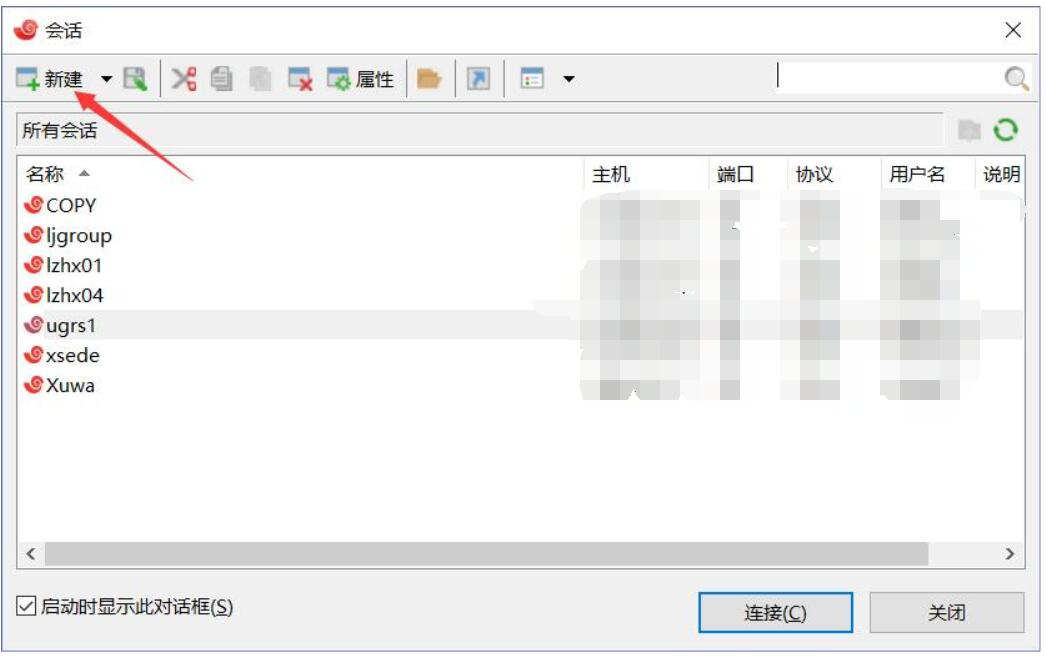
\includegraphics[width = 10cm]{fig/xshell1.jpg}   
          }
          \subfigure[\textbf{\small{XShell6新建会话窗口}}]
          {
            \label{XSHELL6新建}
            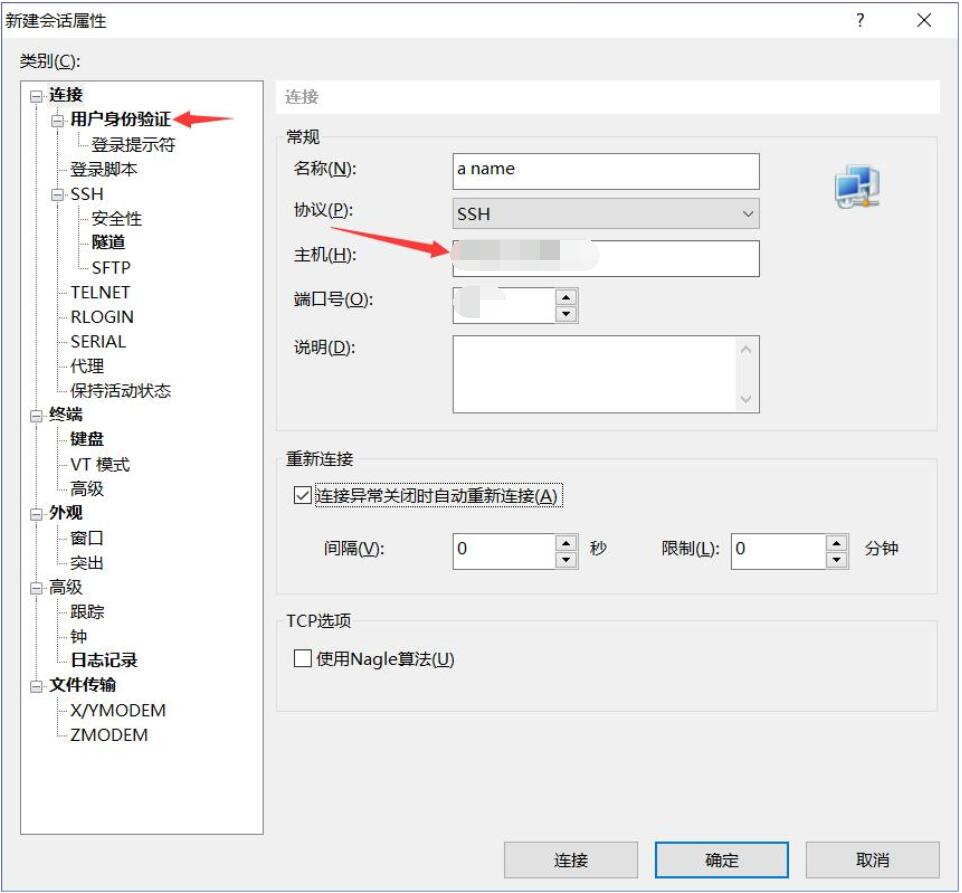
\includegraphics[width = 8cm]{fig/xshell2.jpg}
          }
          \caption{\textbf{XShell连接服务器}}
        \end{figure}
      
        随便起个名字,对应的主机,端口号,用户名,密码请向编者询问\footnote{我们有一个专为入门本科生注册的账号,主要供学习使用,毕设或者读研读博正式在组内工作会有新的账号},(注意:想要成功连接该IP需要浙大内网:ZJUWLAN、有线网络或者RVPN均可)。如果在输入账号密码登录之后见到类似Figure \ref{登录服务器}的界面,就代表已经成功登陆进我们的服务器,并处于\textbf{主目录}(通常用波浪线~表示)下,在光标左侧显示的内容即当前处于ugrs1\_LJ账号下(这个是编者的账号),登录在tc6000节点(主节点,或称登录节点)。
        \begin{figure}
          \centering
          \label{登录服务器}
          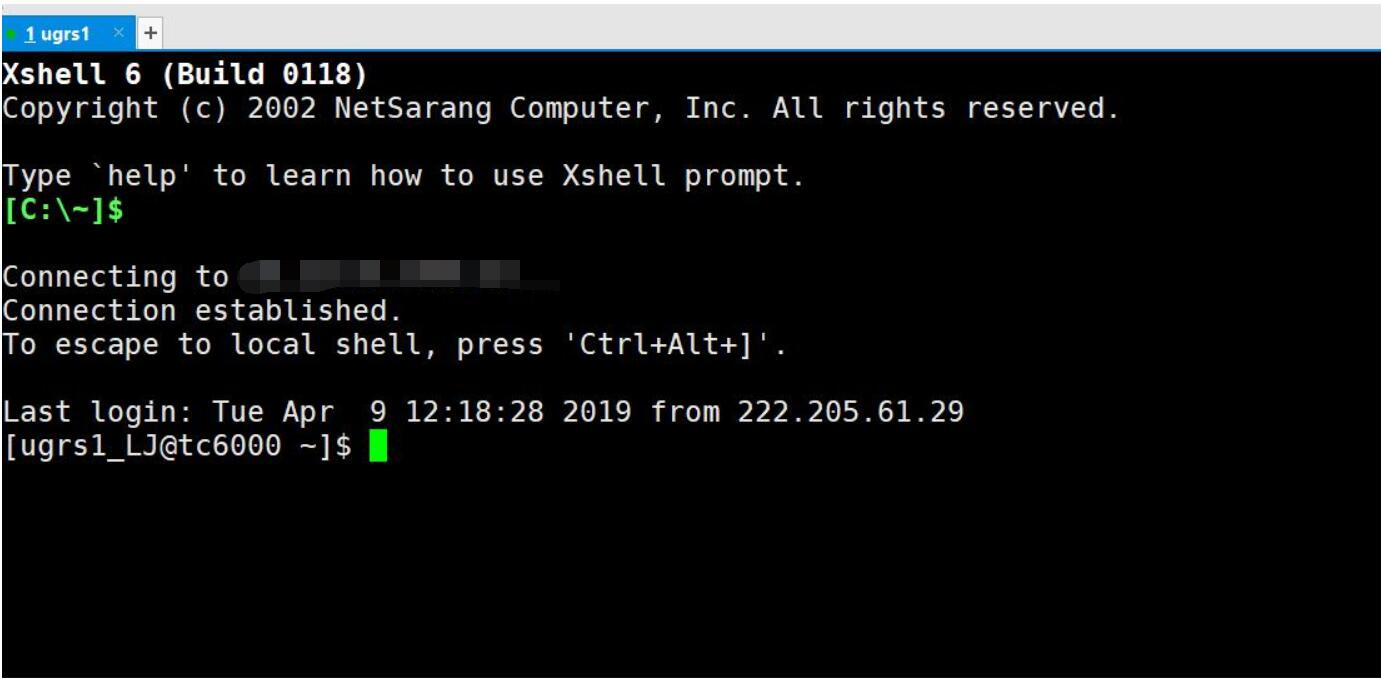
\includegraphics[width = 10cm]{fig/xshell3.jpg}
          \caption{\textbf{成功登陆服务器}}
        \end{figure}
        
        登录服务器之后,就可以按照下一小节的内容进行操作,学习Linux系统的各类指令,和如何在Linux系统下编辑文件,为了安全起见,我们建议每个读者在主目录建立自己的文件夹,然后再自己的文件夹中进行各种操作,避免对他人的文件误操作而造成损失。

      \section{Linux基本操作}
        \begin{description}
          \item[cd]
            进入输入目录的文件夹;
            `cd folder/'
            P.S : `cd ..' 返回上一级文件夹
          \item[ls]
            列出所在文件夹的子文件夹;

          \item[vi / vim]
            打开文件查看内容;vim事实上是一个文本编辑器(比方说这个文档的一部分也是用vim编辑的),下面给出的只是vim常用指令,其实vim功能强大,需要其他操作时可自行查阅相关内容。

            P.S :输入不存在的文件可直接创立该文件;

            vim有一个梗,就是几乎所有的人刚上手的时候都不知道\textbf{该怎么退出}。在这里面稍微描述一下最基本的使用方法:
            \begin{description}
              \item[i / Ins] 如果已经打开了某个文本,那么这两个键中的一个能够允许你对文本作出修改。它左下角会显示 “--INSERT--” 这样的文段,这说明你处在编辑模式,这时候你按出的大部分操作会如同你使用大部分文本编辑器的时候一样,会完整地呈现在你正在修改的文本上。
          
              \item[Esc] 无论你处在何种模式,按了Esc你就能回到正常模式,在该模式下你可以用它自身的快捷键来直接作出一些修改,也可输入命令来完成别的操作(比如\textbf{退出})。

              \item[:q!] 这里‘:’表示进行对vim程序自身的命令,‘q’是quit,‘!’表示强制。也就是输了这个命令并按回车后会强制退出并不保存文件。

              \item[:wq] 以此类推,这个表示的是保存并退出。没错,‘:w’就是进行保存,并不退出。
              
              \item[/xx] 向下搜索xx内容,按n转到下一个,N转到上一个。
              
              \item[?xx] 向上搜索xx内容。  
              
              \item[:sp] 另外打开一个文件,可以使用Ctrl + W按两次的方式在不同文件间切换。  
              
              在编辑模式之外也可以对文本进行操作,常见操作如下(vim指令区分大小写):
              \item[V] 按行选取内容。
              \item[Ctrl + v] 按块选取内容。
              \item[Y] 复制选中内容。
              \item[P] 粘贴复制的内容\footnote{注意:vim里的复制粘贴是仅限在vim编辑器内使用的,而且和系统的复制粘贴(如Xshell提供的)独立}。
              \item[D 或 delete] 剪切选中内容,通常用作删除。
              \item[dd] 剪切当前行,通常用作删除。
            \end{description}
            \sout{好了,现在你也是会用vim的人了!}\footnote{在服务器输vimtutor回车有惊喜!}跟我一起喊,\sout{vim天下第一!}
          \item[pwd]
            显示所在目录路径;它会显示所处目录的绝对路径,而这个绝对路径是你在任何别的目录下都能访问的。从该角度出发,事实上别的几乎所有操作都可以指定绝对路径(比如简单的访问,或者复制,或者在程序里面调用/生成文件)。

          \item[mkdir]
            在所在目录下建立文件夹:
            ‘mkdir levest’ 表示建立名字为‘levest’的文件夹

          \item[cp] 复制文件/文件夹至某个目录
            ‘cp einfield.com slot’ 表示将‘einfield.com’ 在‘slot’文件夹下进行粘贴,如果不存在这个文件夹,则在当前目录下生成一个名为‘slot’的复制

          \item[mv] 原则上它表示将某个东西移动到什么地方,但它的另一个神奇操作在于它可以重命名文件/文件夹(后缀还是要加好)。

          \item[rm] \textbf{ 危险!}这是表示删除操作。
          
          \item[rmdir] 删除空文件夹\sout{,非常安全},文件夹里有任何文件都会报错
          
          \item[man] Linux帮助指令,比如使用man ls可以查看ls指令的全部功能。

          \item[-r] 在Linux中大部分的‘-*’ 表示了所进行的主要命令的附加指令(附加属性\sout{,buff})。像这里‘-r’一般用来表示是对整个文件夹进行操作,像上面的cp,rm 都可以加上-r,但是mv指令比较特殊,mv对文件夹操作不需要-r。

          \item[*] *一般在Linux表示缺省符号,也就是在这里面可以填任何东西。比方说,‘rm *.c’ 表示任何后缀为‘.c’的文件都会被删除\footnote{这就是为什么sudo rm -rf /* 这个梗会流行的原因,{\color{red}{\textbf{务必不要尝试!!!}}}}。

        \end{description}

        读者可以在登录之后所在的主目录下先输入ls指令然后回车,看到当前目录下的文件和文件夹,然后输入“mkdir 文件夹名”的方式创建属于自己的文件夹,然后cd自己的文件夹,之后再这个目录下进行后续的操作。
      
      \section{使用服务器递交任务}
        我们的超算集群,简单地说是由很多的CPU(\textbf{节点})构成的,每个CPU有28个\textbf{核},据说服务器的单核运行效率其实是低于正常个人计算机的,但是优势在计算资源非常多。西溪校区的超算集群主要是王林军老师和洪鑫老师出资,也主要是这两个课题组在使用。王老师占有其中的48个节点,共1344个核。这些节点按照一定的顺序组合成了两个\textbf{队列},分别为ljcluster和ljtest,前者又可以分为wenchang和quantum,使用ljclustat指令可以看到全组的节点使用情况。尽管是为本科生学习练习使用的账号,ugrs3\_LJ账号仍然有对服务器三个节点的访问权限(即ljtest队列)。我们在服务器上递交任务,就是将自己的程序交给这些核去运算,要实现这个靠的是PBS任务管理系统。
        
        计算集群是由多台高性能服务器节点组成的,需要有一套系统能够为我们的计算任务自动分配资源,当计算资源出错的时候,能够避免将任务分到异常节点上去,当计算资源全部用完的时候我们再提交任务,能够有一个排队机制当之前的计算任务完成后自动将排处于队状态的作业自动运行。这就是PBS作业调度系统的主要作用。一个常见的PBS任务脚本如下图所示
        \begin{lstlisting}
          #PBS -N 2butene_PBE_0
          #PBS -l nodes=1:ppn=28
          #PBS -q ljcluster
          #PBS -l walltime=99:60:00
          #PBS -j oe
          nprocs=`cat $PBS_NODEFILE | wc -l`
          
          cd $PBS_O_WORKDIR
          cat $PBS_NODEFILE >> NODEFILE
          source /public/software/profile.d/mpi_openmpi-2.0.0-gnu.sh
          source /public/software/compiler/intel2017/mkl/bin/mklvars.sh intel64
          
          python nac.py > nac.out
        \end{lstlisting}

        这是一个调用PBS管理系统的脚本文件,里面的每一行都有其对应的意思,前几行以\#PBS开头的句子为PBS的调度信息相关的指令,-N 代表作业名,这个脚本的作业名为2butene\_PBE\_0,-l 为计算分配资源,图中为分配了一个节点,28个核,注意到第四行也是这类,分配了这个任务的最大运行时间为99小时60分钟(100小时),-q 代表使用哪个队列,图中即为使用ljtest队列,-j 的一行代表将标准输出信息(o)错误信息(e)合并输出到文件。接下来是bash命令行指令,第一行内容为获取本任务所调用的核数,并将这个数赋值给nprocs(在此脚本中此行为多余的,后面并没有用到nprocs),接下来的两行为打开PBS所在目录(也可以使用绝对目录)和将任务占用的节点信息输出到NODEFILE这个文件中,下面两行为环境变量设置,正常情况下不同任务的环境变量设置是不同的,需要根据任务对应的程序而修改,最后一行为执行命令(python)。需要注意,白色的部分为普通的bash脚本,因此可以根据需要任意添加。

        写完PBS文件之后(本例子中文件名即为PBS,可以按需修改),只需要执行“qsub PBS”指令就可以将这个脚本递交给PBS系统,而PBS系统负责根据这个脚本的内容为你分配计算资源,进行计算。希望查看自己的任务,可以使用“qstat”指令,可以打出所有正在服务器运行的任务,希望检索特定队列可以用“-a”,希望进行搜索可以在指令后添加额外的grep指令,举例:如果你希望输出所有在ljtest队列上运行的信息带有ugrs3的任务,指令是“qstat -a ljtest |grep ugrs3”。所有任务的后面会有一个status,R代表正在运行,Q代表正在排队等待运行,C代表运行完成(不代表算对,有可能是由于错误退出),E代表错误退出,H代表被挂起,H的任务即使排队到了资源也不进行计算,先让他之后的任务计算。

        此外,PBS系统还有诸多指令(如常用的qdel和qhold等),诸多功能,诸多环境变量可以调用,鉴于递交任务实际操作的重要性,这里不再赘述,如果在实际操作过程中希望有更多了解,可以参阅浙江大学西溪校区化学系HPC超算平台介绍(可在超算QQ群的群文件中找到)中的Gridview PBS作业调度使用说明。
      
    \chapter{数学基础}

      本章包含了在王老师课题组可能用到的数学知识,但是并不是所有人所有方向都非常重要。阅读此章内容前,我们默认你掌握了基础的数学知识:单变量微积分,多元函数微积分,基础线性代数。如果自认为对此比较熟悉,可以有用到相关知识的时候再回来检索查看,如果不熟悉,还是建议阅读本章内容。对于一部分有一定意义但影响阅读连贯性的内容(例如部分证明及拓展应用),我们会将其列于附录中。\textbf{本指南不适合完全没学过线性代数的同学,如果想完整学习线性代数请参阅相关教材。}

      \section{数学回顾}
      
        数学基础的第一小节将关注于最基础的数学内容,主要是最基础的复数概念、线性代数和微积分的一些知识,由于长时间不用可能有所生疏,我们就在这里作简单的回顾。并且把线性代数学习中常用的实数问题推广到复数的情况下。熟悉此节内容的同学可以直接跳过。

        \subsection{复数及复变函数基础}

          相关内容参考\cite{methods_in_math_phys_liang}。

          {\color{red}{\textbf{以下内容针对对于复数及复变函数非常不熟悉的读者,更深入的内容将在后面出现。}}}
          
          复数是实数的拓展。让我们先回顾一下从小到大的数学的学习,来看一下我们(也是整个人类)是怎么认识数的。
          
          首先认识的是正整数,正整数$\mathbb{Z}^+$对加法封闭\footnote{本节中,封闭的意思是对集合中的数进行某种运算的结果仍然在该集合内。},但是对于减法就不封闭了,于是人们引入了负整数,组成了对加减法都封闭的整数$\mathbb{Z}$。整数对乘法也封闭,但是对非零除法则不封闭,于是数扩张为了有理数$\mathbb{Q}$。有理数对加减乘除都封闭,但是对于例如对角线长度、圆的周长之类的问题时就不好解决了,从而引入了无理数\sout{以及各种测度}$\mathbb{R}$。到目前为止看起来可以告一段落,但是,当人们求解实系数代数方程的时候,发现其根不一定是实数,从而引入了虚数,组成了复数$\mathbb{C}$。简单的说,数的扩充是为了更高级的运算,而复数的意思是对代数方程求根封闭。数学王子高斯证明了,在复数域上,$N$次方程有$N$个根\footnote{此即为\textbf{代数基本定理}}。
          
          引入复数的核心就是单位虚数$i$,定义为
          \begin{equation}
            i=\sqrt{-1}
          \end{equation}
          这个定义想必对于很多人都是平凡的,对其历史不再赘述。一个一般的复数$z$,可以表示为
          \begin{equation}
            z=x+iy
          \end{equation}
          这称为复数的\textbf{代数式},其中$x$被称为\textbf{实部},$y$被称为\textbf{虚部}。
          \begin{equation*}
            \begin{cases}
              x=\Re(z)\\
              y=\Im(z)
            \end{cases}
          \end{equation*}
          于是从某种意义上来说,复数可以看成是一个二元有序实数对$(x,y)$。复数的几何表示也自然而然地对应一个二维平面\footnote{即\textbf{复平面}}。

          对于每一个$z=x+iy$,存在一个复数$x-iy$。这个复数与原复数实部相同而虚部符号相反,其被称为$z$的共轭复数,记为$z^*$\footnote{也有一些书上采用记号$\bar{z}$}。复数和其共轭复数的乘积必然是实数,对此的证明是平凡的,利用$i$的定义即可。
          
          复数也可以用极坐标$\rho$和$\phi$来表示。
          \begin{equation}
            \begin{cases}
              \rho=\sqrt{x^2+y^2}\\
              \phi=\arctan(\frac{y}{x})
            \end{cases}\ \begin{cases}
              x=\rho\cos\phi\\
              y=\rho\sin\phi
            \end{cases}
          \end{equation}
          则复数可以表示为\textbf{三角式}
          \begin{equation}
            z=\rho\qty(\cos\phi+i\sin\phi)
          \end{equation}
          或\textbf{指数式}
          \begin{equation}
            z=\rho e^{i\phi}
          \end{equation}
          其中$\rho$称为复数的\textbf{模},而$\phi$称为复数的\textbf{辐角}。若$0\leq\phi<2\pi$,则称为\textbf{辐角主值}。
          \begin{equation}
            \begin{cases}
              \rho=\abs{z}\\
              \phi=\arg\qty(z)
            \end{cases}
          \end{equation}
          以下运算结论利用定义即可得到,在此直接给出结论:对于
          \begin{equation*}
            \begin{cases}
              z_1=x_1+iy_1=\rho_1 e^{i\phi_1}\\
              z_2=x_2+iy_2=\rho_2 e^{i\phi_2}
            \end{cases}
          \end{equation*}
          有
          \begin{eqnarray}
            z_1+z_2&=&\qty(x_1+x_2)+i\qty(y_1+y_2)\Rightarrow\abs{z_1+z_2}\leq\abs{z_1}+\abs{z_2}\\
            z_1-z_2&=&\qty(x_1-x_2)+i\qty(y_1-y_2)\Rightarrow\abs{z_1-z_2}\geq\abs{z_1}-\abs{z_2}\\
            z_1z_2&=&\qty(x_1x_2-y_1y_2)+i\qty(x_1y_2+x_2y_1)=\rho_1\rho_2 e^{i\qty(\phi_1+\phi_2)}\\
            \frac{z_1}{z_2}&=&\frac{x_1x_2+y_1y_2}{x_2^2+y_2^2}+i\frac{x_2y_1-x_1y_2}{x_2^2y_2^2}=\frac{\rho_1}{\rho_2}e^{i\qty(\phi_1-\phi_2)}
          \end{eqnarray}
          复数减法是加法的逆运算,除法是乘法的逆运算;加法满足交换律、结合律,乘法满足交换律、结合律、分配律,这与实数是一致的。对于$n\in\mathbb{Z},z=\rho e^{i\phi}$,
          \begin{eqnarray}
            \label{z_n}
            z^n=\rho^ne^{in\phi}\\
            \label{sqrt_n_z}
            \sqrt[n]{z}=\sqrt[n]{\rho}e^{i\frac{\phi}{n}}
          \end{eqnarray}
          对于\ref{z_n},要注意区别$\abs{z}^2$,$\abs{z^2}$和$z^2$;对于\ref{sqrt_n_z},注意到由于辐角$\phi$改变$2\pi$之后复数仍然是同一个数,因此原则上$\sqrt[n]{z}$可以有$n$个取值,这是不同于实数开根号的。

          下面简要地介绍一下复变函数。对于某一复数集$E$(比如全体复数集$\mathbb{C}$),对于集合中任一复数$z$,按照一定的规律,存在\textbf{一个或多个}复数值$w$与之对应,则称$w$是$z$的函数,该函数称为\textbf{复变函数},$z$为$w$的\textbf{宗量}\footnote{本质上和实变函数的\textbf{自变量}没有区别},$E$为定义域,记为
          \begin{equation}
            w=f\qty(z),\ z\in E
          \end{equation}
          举一些具体而常见的例子。
          \begin{eqnarray*}
            f\qty(z)&=&a_0+a_1z^1+a_2z^2+\cdots+a_nz^n,\ n\in\mathbb{Z}^+\\
            f\qty(z)&=&\frac{a_0+a_1z^1+a_2z^2+\cdots+a_nz^n}{b_0+b_1z^1+b_2z^2+\cdots+b_mz^m},\ m,n\in\mathbb{Z}^+\\
            f\qty(z)&=&\sqrt{z-a}\\
            e^z&=&e^xe^{iy}\\
            \sin z&=&\frac{e^{iz}-e^{-iz}}{2i}\\
            \cos z&=&\frac{e^{iz}+e^{-iz}}{2}\\
            \sinh z&=&\frac{e^z-e^{-z}}{2}\\
            \cosh z&=&\frac{e^z+e^{-z}}{2}\\
            \ln z&=&\ln(\abs{z}e^{i\arg{z}})=\ln\abs{z}+i\arg\qty(z)\\
            z^s&=&e^{s\ln z},\ s\in\mathbb{C}
          \end{eqnarray*}
          可以看出,$\sin$和$\cos$具有实周期$2\pi$,且其\sout{绝对值}模不再小于等于$1$;$e^z$,$\sinh z$和$\cosh z$具有纯虚周期$2\pi i$;对数函数$\ln z$具有无穷多取值\footnote{和开方可以多值原因相同,即辐角可以任意改变$2\pi$之后复数仍然是同一个数},且负数的对数在复数域下有意义。

          前述已经提到,复数可以看成二元有序实数对,即$z=\qty(x,y)$,这可以拓展到复变函数上,即将复变函数$f(z)$分为实部和虚部两部分,记为
          \begin{equation}
            f\qty(z)=u\qty(x,y)+iv\qty(x,y)
          \end{equation}
          即一对二元实变函数,并且可以适用许多实变函数论的性质\sout{然而本教程并不会涉及相关内容}。但是,我们仍然需要研究完整的复变函数而不是两个孤立的二元实变函数,这一点可以很明显地体现在复变函数的导数上。

          让我们回忆以下多变量微积分的内容。二元实变函数$f(x,y)$只有偏导数$f_x=\pdv{f}{x}$和$f_y=\pdv{f}{y}$,以及全微分$\dd{f}=f_x\dd{x}+f_y\dd{y}$\footnote{让我们暂时忘掉那些小量、邻域之类的鬼东西吧,物理和化学上的函数\textbf{原则上}都是无穷阶可导的光滑函数\sout{,当然,有原则就会有例外}。}。这很好,但是复变函数有更好的,导数:
          \begin{equation}
            \dv{f}{z}=f'\qty(z)=\lim_{\Delta z\rightarrow0}{\frac{f\qty(z+\Delta z)-f\qty(z)}{\Delta z}}
          \end{equation}
          当然,类似于二元实变函数的极限,我们需要极限存在并且与$\Delta z\rightarrow0$无关。于是,我们就有了一系列很棒的性质。
          \begin{equation*}
            \begin{cases}
              \dv{z}\qty(w_1\pm w_2)=\dv{w_1}{z}\pm\dv{w_2}{z}\\
              \dv{z}\qty(w_1w_2)=\frac{\ud w_1}{\ud z}w_2+w_1\frac{\ud w_2}{\ud z}\\
              \dv{z}\qty(\frac{w_1}{w_2})=\frac{w'_1w_2-w_1w'_2}{w_2^2}\\
              \dv{w}{z}=\qty(\dv{z}{w})^{-1}\\
              \dv{z}F\qty(w)=\dv{F}{w}\cdot\dv{w}{z}
            \end{cases}\ \begin{cases}
              \dv{z}z^n=nz^{n-1},n\in\mathbb{Z}\\
              \dv{z}e^z=e^z\\
              \dv{z}\sin z=\cos z\\
              \dv{z}\cos z=-\sin z\\
              \dv{z}\ln z=\frac{1}{z}
            \end{cases}
          \end{equation*}
          可以看出,复变函数和实变函数非常类似但是又有区别。

          关于复变函数就暂时介绍到这里,后面会有更加详细而繁难的内容。

        \subsection{线性空间,线性映射与矩阵}

          对于矢量空间的数学定义,我们不做仔细讨论,简单地说,我们在某个数域$\mathbb{F}$\footnote{下文中$\mathbb{F}=\mathbb{R}$或$\mathbb{C}$,不再赘述}上定义了一个非空集合$V$,这个$V$中的元素满足加法交换律,对于数乘运算满足结合律,分配律等,而且数乘和加法的运算关于集合$V$是封闭的,我们就称$V$是一个线性空间,或者矢量空间,矢量空间内的元素称为矢量/向量。我们按照定义证明物理中的三维空间矢量是实数域上定义的线性空间,另外我们可以在矢量空间中定义内积和两个矢量的夹角,普适定义不再展开,本指南中将用最朴素的内积\footnote{$\mean{a,b}=\sum_{i=1}^n{a_i^*\times b_i},\ a,b\in\mathbb{F}^n$},长度\footnote{矢量$a$的长度$\norm{a}=\sqrt{\mean{a,a}}$}和矢量夹角\footnote{$\theta_{a,b}=\arccos(\frac{\mean{a,b}}{\norm{a}\cdot\norm{b}})$}定义方式,在三维实空间下就是我们熟知的矢量模和夹角形式。

          对于线性空间中的向量,我们可以做线性组合,对于线性空间中的元素$\qty{\vb*{a}_1,\vb*{a}_2,\vb*{a}_3,\dots,\vb*{a}_N}$,如果存在不全为零的系数$\qty{\lambda_i}$使得
          \begin{equation}
            \lambda_1\vb*{a}_1+\lambda_2\vb*{a}_2+\cdots+\lambda_N\vb*{a}_N=\vb*{0}
          \end{equation}
          则称这个矢量组$\qty{\vb*{a}_1,\vb*{a}_2,\vb*{a}_3,\dots,\vb*{a}_N}$的元素\textbf{线性相关},否则称为\textbf{线性无关}。线性相关的向量意味着其中一个可以用其他向量的线性组合表示,也就是他们并不是独立的。在一个线性空间中可以找到的最大的线性无关向量组的个数称为这个线性空间的维度,比如在三维空间内我们最多可以找到三个线性无关的矢量,通常选用三个单位正交矢量。需要注意,线性无关不代表正交,二维空间内夹角为1度的两个矢量也是线性无关的\footnote{但是总可以通过Gram-Schmidt正交化或者其他正交化方法从一组线性无关的矢量构建同样个数的正交矢量}。这个最大的线性无关矢量组,就可以作为这个空间的基矢量,线性空间中的任何一个矢量都可以写成基矢量的线性组合。
          
          这个线性组合的系数通常是我们所关心的东西,在一组基矢量$\qty{\vec{e}_i}$下,这个线性空间的任何向量都可以表示为
          \begin{equation}
            \vec{f}=\sum_i^N{c_i\vec{e}_i}
          \end{equation}
          在定义了基矢量之后,我们没有必要每次都把基矢量写出来,因为一组完备的系数组就足够描述这个矢量。我们通常用一个含有N个(空间维度)元素的数组来表示一个矢量,比如说三维空间中的$(c_1,c_2,c_3)$。在这之后,我们可以定义一种映射$\mathcal{O}$,它把线性空间$V_1$内的元素映射到另一个线性空间$V_2$下,并且满足线性性,即
          \begin{equation}
            \mathcal{O}\qty(\lambda\vb*{a}+\mu\vb*{b})=\lambda\mathcal{O}\qty(\vb*{a})+ \mu\mathcal{O}\qty(\vb*{b})
          \end{equation}
          则称$\mathcal{O}$是从$V_1$到$V_2$的\textbf{线性映射}\footnote{也称为\textbf{线性变换}},如果$\mathcal{O}$是把一个矢量映射到自己的线性空间,则称为\textbf{线性算子}。我们知道,如果这个映射对于矢量空间的基矢量定义好了,所有矢量的映射就都定义好了。我们对基矢量中的$\vec{e}_i$做线性变换,由于其仍然位于这个线性空间下,所以变换完的矢量$\mathcal{O}(\vec{e}_i)$可以写成所有基矢量的线性组合:
          \begin{equation}
            \mathcal{O}(\vec{e}_i)=\sum_j^N{O_{ij}\vec{e}_j}
          \end{equation}
          式中的$O_{ij}$可以认为是一个矩阵的矩阵元,这样一个线性变换就和一个矩阵一一对应\footnote{线性算子对应方矩阵,线性映射对应全部矩阵},而这个映射的逆映射也就与这个矩阵的逆矩阵相对应。同样的,对于一个矩阵
          \begin{equation}
            \vb*{A}=\mqty(
              A_{11} & A_{12} & \cdots & A_{1 M} \\
              A_{21} & A_{22} & \cdots & A_{2 M} \\
              \vdots & \vdots & {} & \vdots \\
              A_{N 1} & A_{N 2} & \cdots & A_{N M}
            )
          \end{equation}
          都对应着一个线性映射,对于一个写成列向量的$M$维矢量
          \begin{equation}
            \vb*{a}=\mqty(
              a_1 \\
              a_2 \\
              \vdots \\
              a_M
            )
            \label{column vector}
          \end{equation}
          矩阵$\vb*{A}$可以将其转化为一个$N$维矢量$\vb*{b}$
          \begin{equation}
            \begin{aligned}
              \vb*{A} \vb*{a}&=\vb*{b} \\
              b_i=\sum_{j=1}^M{A_{i j} a_j} &\quad i=1,2, \ldots, N
            \end{aligned}
            \label{linear transformation}
          \end{equation}

          有一种线性算子,它满足在变换前后矢量的模长不变,这个性质保证了原本正交归一的基矢量在变换后是另一组正交归一的基矢量,这个性质在量子力学的表象变换中至关重要,这类变换称为\textbf{正交(orthogonal)变换},正交变换对应的矩阵为\textbf{正交矩阵}\footnote{不同书的名称不同,也有称为\textbf{等距同构}},即满足
          \begin{equation}
            \vb*{A}\vb*{A}^\mathsf{T}=\vb*{I}
          \end{equation}
          其中$^\mathsf{T}$为转置符号,$\vb*{I}$为单位矩阵,容易证明,满足这样条件的矩阵对应的线性变换是保持矢量模长的,证明\sout{留作习题}可见于附录\ref{orthogonal_matrix_properties}\footnote{该部分内容可能需要对复数以及复空间有一定的了解,对此不了解的请先阅读正文的相关章节}。

        \subsection{行列式}
          行列式在线性代数的书中有多种等价定义,为了与讲解量子化学推导内容的一致性,我们选用排列法的定义,即对于一个方矩阵
          \begin{equation}
            \det\qty(\vb*{A})=\abs{\vb*{A}}=\mdet{
              A_{11} & \cdots & A_{1 N} \\
              \vdots & {} & \vdots \\
              A_{N 1} & \cdots & A_{N N}
            }=\sum_{i=1}^{N !}{\qty(-1)^{p_i} \mathscr{P}_i A_{1i_1} A_{2i_2} \cdots A_{N i_N}}
            \label{determinants definition}
          \end{equation}
          其中$\mathscr{P}_i$是排列算符,它的意义是给出一种列指标$1,2,3,\dots,N$的排列,求和就是关于所有的$N!$种排列求和,$p_i$是从自然序排列(1,2,3,\dots,N)出发得到排列$\mathscr{P}_i$所需要的近邻交换操作的个数。看似非常复杂,让我们以$3\times3$矩阵为例说明这个操作是如何实现的。

          对于$3\times3$矩阵的矩阵元乘积$A_{1i_1} A_{2i_2}A_{3i_3}$的排列总有$3!=6$种,即$i_1,i_2,i_3$分别等于$1,2,3$,$1,3,2$,$2,3,1$,$2,1,3$,$3,1,2$和$3,2,1$,接下来就是计算每种排列对应的$p_i$,即从$1,2,3$实现该排列所需要的近邻交换操作的个数,分别是$0,1,2,1,2,3$\footnote{你可能算出来跟我差一个偶数,但根据式(\ref{determinants definition})这不重要},所以$3\times3$矩阵的行列式计算表达式为
          \begin{equation}
            \det(\vb*{A})=A_{11} A_{22}A_{33}-A_{11} A_{23}A_{32}+A_{12} A_{23}A_{31}-A_{12} A_{21}A_{33}+A_{12} A_{21}A_{32}-A_{13} A_{22}A_{31}
          \end{equation}
          可以看到与用Laplace展开定义的结果一致。

          矩阵的行列式最重要的一些性质有:如果矩阵不满秩(这个矩阵的每一列或者每一行单独写成一个向量,他们线性相关),矩阵的行列式为0,矩阵就没有对应的逆矩阵\footnote{矩阵有逆矩阵,等价于行列式不为0,没有逆矩阵的矩阵对应的线性映射也是不可逆的(损失信息)};$\abs{\vb*{A B}}=\abs{\vb*{A}}\abs{\vb*{B}}$;任意交换行列式中的两列(行),矩阵行列式反号。

        \subsection{特征值与特征向量}
          在线性代数课程中,特征值与特征向量可能不被特别重视,\sout{当然主要原因是需要重视的东西太多了,}但是在物理学、工程的诸多应用中,特征值与特征向量几乎是整个线性代数最常用的一块知识点。

          线性代数中定义,如果矩阵$\vb*{A}$右乘一个向量$\vb*{X}$恒等于一个数$\lambda$乘以这个向量
          \begin{equation}
            \vb*{AX}=\lambda\vb*{X}
            \label{eigen definition}
          \end{equation}
          那么向量$\vb*{X}$称为矩阵$\vb*{A}$的对应特征值$\lambda$特征向量。如何求解特征值和特征向量其实非常简单,先假设特征向量存在,就有
          \begin{equation}
            \vb*{AX}-\lambda\vb*{I}\vb*{X}=\qty(\vb*{A}-\lambda\vb*{I})\vb*{X}=0
            \label{eigen definition2}
          \end{equation}
          当$\vb*{X}$不是零向量时,要求左边乘以它的矩阵的行列式为0,由此得到
          \begin{equation}
            \det\qty(\vb*{A}-\lambda\vb*{I})=0
            \label{eigen equ}
          \end{equation}
          就可以求出特征值,将特征值代入(\ref{eigen definition})或(\ref{eigen definition2})就可以求出对应的特征矢量。其实可以看到一个特征值对应的特征矢量构成了一个线性空间,称为特征子空间。

          在应用中,我们经常需要将一个矩阵对角化,即通过线性变换使得矩阵变成对角阵,对角化通常是使用特征值与特征向量的方法。如果$n\times n$矩阵$\vb*{A}$有$n$个特征值,对应$n$个特征向量,\sout{物理里的矩阵性质都很好的,}首先求出矩阵对应的特征值和(模为1)特征向量,将这些特征向量按列向量的形式组合成一个矩阵
          \begin{equation*}
            \vb*{S}\equiv\mqty[x_1 & \cdots & x_n]
          \end{equation*}
          计算矩阵$\vb*{A}$乘以$\vb*{S}$
          \begin{equation}
            \begin{aligned}
              \vb*{A S}=\vb*{A}\mqty[x_1 & \dots & x_n]=\mqty[\lambda_1 x_1 & \cdots & \lambda_n x_n]= \\
              \mqty[x_1 & \dots & x_n] \mqty[
                \lambda_1 & {} & {} \\
                {} & \ddots & {} \\
                {} & {} & \lambda_n
              ]=\vb*{S }\Lambda
            \end{aligned}
          \end{equation}
          其中$\Lambda$是由矩阵$\vb*{A}$的$n$个特征值构成的对角矩阵,所以我们得到
          \begin{equation}
            \vb*{S^{-1}AS}=\Lambda
          \end{equation}
          这就得到了一个对角阵。

          什么样的矩阵可以对角化是一个很复杂的问题,我们只给出一个充分条件,实对称矩阵(矩阵和它的转置相等)一定可以在实数范围内对角化得到实数特征值,并且不同特征值对应的特征矢量是正交的\footnote{这是实谱定理的一部分,参考附录\ref{spectral_theorem}}。而与之相反的是反对称矩阵(矩阵和它的转置相差负号),反对称矩阵在实数范围内无法对角化\footnote{除了极少数反对称矩阵,如矩阵元全是零的零矩阵$\vb*{O}$}。
    
        \subsection{向复数域推广}
          \label{expansion_to_complex_field}
          接下来做推广,上述矢量空间均为定义在实数域上的,可以不做任何额外修正,完全转化到复数域,矩阵元,向量的分量,都可以为复数。在这个意义下,我们习惯将一个矢量写成列矢量的形式,就像式(\ref{column vector})那样。我们定义矩阵和向量的\textbf{共轭转置}\footnote{也称为\textbf{厄米共轭}},用$^\dagger$符号表示
          \begin{equation}
            \begin{aligned}
              \qty(\vb*{A}^\dagger)_{i j}=A_{j i}^* \\
              \vb*{a}^\dagger=\mqty(a_1^*\ a_2^*\ \cdots\ a_M^*)
            \end{aligned}
          \end{equation}
          在复数域的线性空间内,矢量的内积定义为行矢量和列矢量的乘积
          \begin{equation}
            \mean{a,b}=\vb*{a}^\dagger\vb*{b}=\mqty(a_1^*\ a_2^*\ \cdots\ a_M^*) \mqty(
              b_1 \\
              b_2 \\
              \vdots \\
              b_M
            )=\sum_{i=1}^M{a_i^* b_i}
            \label{inner product in row and column }
          \end{equation}
          可以看到,$\vb*{a}=\vb*{b}$时,我们可以定义的矢量模平方,在复数域上刚刚好是矢量每个元素的模的平方和。在复数域下,矩阵原本的很多性质都得到保持,只是简单地向复数域的推广,毕竟实数域是复数域的一部分,向更全的集合的推广往往能得到更加普适的性质。

          在复数域上有很多特殊的矩阵,比如\textbf{幺正(unitary)矩阵}\footnote{由于翻译问题部分教材称为\textbf{酉矩阵}},是正交矩阵的推广,满足
          \begin{equation}
            \vb*{A}\vb*{A}^\dagger=\vb*{I}
            \label{unitary def}
          \end{equation}
          在复数域上保持矢量模不变的线性变换,对应的就是幺正矩阵。而实对称矩阵的推广就是\textbf{厄米(Hermite)矩阵}\footnote{也称为\textbf{自伴(self-adjoint)矩阵}},厄米矩阵定义多种多样,我们取其中最简单的一种,即
          \begin{equation}
            \vb*{A}=\vb*{A}^{\dagger}
          \end{equation}
          可以看出,如果矩阵元都是实数,幺正矩阵就是正交矩阵,因此在复数范围内的保持矢量模长不变的变换就是\textbf{幺正变换},它在量子力学的推导中极为重要;厄米矩阵就是实对称矩阵。厄米矩阵和实对称矩阵的性质相似:具有实数的特征值,并且不同特征值对应的特征向量正交。厄密矩阵的另一种定义为\footnote{也是“自伴”这一名称的来源,$\vb*{A}$的\textbf{伴随矩阵}$\vb*{A}^\dagger$的定义为$\mean{u,\vb*{A}v}=\mean{\vb*{A}^\dagger u,v}$。这一定义是从内积出发的,和从算符的矩阵形式出发得到的厄米共轭矩阵是等价的。}
          \begin{equation}
            \mean{u,\vb*{A}v}=\mean{\vb*{A}u,v}
          \end{equation}

          最后讨论一种特殊的矩阵,正规矩阵,定义为
          \begin{equation}
            \vb*{A}\vb*{A}^\dagger=\vb*{A}^\dagger\vb*{A}
          \end{equation}
          从这个定义看出,厄米矩阵和幺正矩阵都是正规矩阵。我们介绍在复数域上正规矩阵的谱定理,证明\sout{留作习题}参考附录\ref{spectral_theorem}。
          \begin{theorem}
            设我们在复数域上定义线性内积空间$V(F),F=C$且$\vb*{A}$是这个线性内积空间的一个线性算子,则以下条件等价:\\
            1.$\vb*{A}$是正规的;\\
            2.$V$有一个由$\vb*{A}$的本征向量构成的正交归一基;\\
            3.$\vb*{A}$在$V$的某个正交归一基下是对角矩阵。
          \end{theorem}
          这个定理的存在对量子力学至关重要,我们这里只简单的提一点:量子力学中的力学量(如坐标、动量和能量)都是由厄密算符表示的。至于更多的内容,将留待后面的章节详述。

        \subsection{向函数空间推广}
          \label{expantion_to_function_space}
          学完线性代数大家都知道,一个线性空间可以由一组基矢量来描述,我们生活的三维空间可以用三个相互正交的单位矢量做展开,看起来都是平凡的。但是线性空间的定义远远不限于通常的“矢量”的空间,你学完现代的时候可能并不会意识到函数空间其实也是线性空间。

          以最简单的多项式为例,首先我们写成一个任意的n阶多项式
          \begin{equation}
            P_n\qty(x)=\sum_{i=0}^n{c_i x^i}
          \end{equation}
          可以看到,它也是由n个小函数$\qty{1,x,x^2,x^3,\dots,x^n}$线性组合成的,而且如果这个多项式恒等于0的话,我们必须要求每一个系数$c_i$都等于0,如果回忆一下线性无关的定义,我们就会发现这几个函数其实是线性无关的,而且这n个函数已经能表示出任意一个n阶多项式,你可以回顾线性空间的定义,n阶多项式的集合其实是一个n维线性空间,就可以选用$\qty{1,x,x^2,x^3,\dots,x^n}$作为这个线性空间的一个基。那对于上面那个多项式,我们就可以将其写作一个矢量:
          \begin{equation}
            P_n\qty(x)=\qty[c_0,c_1,\dots,c_n]
          \end{equation}

          接下来,我们做一个不那么平凡的推广,那就是任意多项式的集合也是一个线性空间,维数为无穷\footnote{从有限到无穷的推广通常,在数学上不能这么随意,但是在物理上则比较随意……嗯},即$\qty{1,x,x^2,x^3,\dots,x^n}, n\rightarrow\infty$。在这种情况下,它所定义的就不只是多项式了,而是全体函数。对于一个一般的函数,可以用Taylor展开的方式写出这个基下的展开形式。例如,对于$e^x$,我们可以很容易地得到
          \begin{equation}
            e^x=1+x+\frac{x^2}{2}+\frac{x^3}{3!}+\cdots+\frac{x^n}{n!}+\cdots=\sum_{n=0}^\infty{\frac{x^n}{n!}}
          \end{equation}
          那么,对于基函数$x^n$而言,其对应的展开系数即为$\frac{1}{n!}$,这和将矢量展开为基向量的线性组合是非常类似的。在这种情况下,我们就可以将其写作一个无穷维的矢量,即
          \begin{equation}
            e^x=\qty[\frac{1}{0!},\frac{1}{1!},\frac{1}{2!},\frac{1}{3!},\dots,\frac{1}{n!},\dots]
          \end{equation}

          那么这组基矢量(或者说基函数)是否正交归一呢?这就涉及到一个复杂的问题,函数的内积怎么定义,我们上文中其实没有展开内积的严格定义,只是给出了对于一般矢量,点积就是内积。我们此处也不深究内积的高级定义,只是给出对于函数空间的内积的一种常用定义方式,即
          \begin{equation}
            \mean{f,g}=\int_a^b{\dd{x} f\qty(x)g\qty(x)}
          \end{equation}
          如果这两个函数是复函数,上式的定义中通常将$f\qty(x)$换为它的复共轭$f^*\qty(x)$,如果取积分是从$-1$到$1$,可以看到上面我给出的这组基是不正交的(当然这不影响他们线性无关)。对于有无穷多个函数构成的基矢量组,我们也可以用类似Gram-Schmidt 正交化的方法来定义一组正交基,读者如果有兴趣,可以从我们给出的这组基出发,将积分范围限定在$\qty[-1,1]$上做Gram-Schmidt正交化,就会得到勒让德多项式(会相差一个系数,但是系数不影响正交性)。

          同样,很多函数空间,比如全体平方可积函数(函数平方在全空间积分为有限值)的集合,全体连续函数的集合,全体一阶导连续函数的集合等等,都可以构成一个线性空间,当然它们都是无穷维的。我们常见的基函数也有很多种,比如上面提到的勒让德多项式,它虽然复杂,但只是一组多项式而已,如果大家的微积分学的不错,应该会想到,傅里叶级数其实就是把函数在三角函数基上展开,并且求解这个展开系数。我们会在\ref{fourier_transformation}一节中详细地讲述相关内容。
          
          波函数通常被说成是一个希尔伯特空间\footnote{数学上对希尔伯特空间的定义为“完备线性内积空间”,量子力学中通常使用的是全体平方可积的函数的集合作为希尔伯特空间,这事实上是希尔伯特空间的一个特例}的态矢量,所以有时候波函数写成函数形式,有时候又可以用矩阵力学的语言写成向量形式。通过上述说明,你可以认识到,如果我们找到了一个合适的函数基组,函数和向量可以是等价的。
    
      \section{符号使用}
        在量子力学相关领域,人们使用\textbf{左矢}(bra)和\textbf{右矢}(ket)来描述一个“状态”。我们可以先简单地认为右矢代表了一个列向量,左矢则代表了一个行向量。它们是这么表示的:
        \begin{equation*}
          \ket{\xi} \rightarrow \text{右矢}, \bra{\xi} \rightarrow \text{左矢}    
        \end{equation*}
        我们知道,一个行向量和列向量相乘能够得到一个实数,这也可以理解为两个向量进行内积的过程。那么在左矢和右矢的形式下,对于两个向量的内积,我们首先写成左矢和右矢的形式,即左矢$\vb*{\xi}_1=\bra{\xi_1}$和右矢$\vb*{\xi}_2=\ket{\xi_2}$,那么其内积可以简单地写作
        \begin{equation*}
          \mean{\vb*{\xi}_1,\vb*{\xi}_2}=\bra{\xi_1}\ket{\xi_2}
        \end{equation*} 
        那么某种程度上,左矢代表的是右矢的共轭转置,左矢和右矢相作用得到的是两者的内积。

        当然量子力学远不止于此,它有可能包括了各种奇奇怪怪的东西,使得它并不能完全用向量来描述。比如说,算符。算符是作用在矢量上的。在线性代数里我们可以认为算符是一个矩阵;如果你学过张量分析/矢量代数,你还可以认为它代表了一个张量。当然,我们简单的先认为算符是一个矩阵。有些人们喜欢用$\hat{Q}$类似这样的形式来表达一个算符(也就是加个帽子),也有些人喜欢用粗体,比如$\vb*{Q}$这样来表达,也有人不加任何东西\footnote{没错就是发明这一套符号系统的\Large{Dirac}大佬。},只要它“在该在的地方”就可以识别为一个算符。算符放在左矢的右边,或者右矢的左边,或者左矢和右矢的中间,也就是
        \begin{equation*}
          \hat{Q}\ket{\xi},\ \bra{\xi}\hat{Q},\ \mel**{\xi_1}{\hat{Q}}{\xi_2}   
        \end{equation*}
        到了这里,当然就会出现作用顺序(方向)的问题。不过其实这一套和线性代数非常相像\footnote{事实上这一套就是线性代数——也就是海森堡开发的矩阵力学的核心,量子力学就是线性代数(并不是)},算符默认是作用在右边的,如果需要作用在左矢,那么对应的是原算符的厄米共轭\footnote{用$\hat{Q}^\dagger$来表达,回忆一下\ref{expansion_to_complex_field}一节中对厄米共轭的定义}作用在这个左矢对应的右矢上,然后再将得到的右矢转换成对应的左矢。

        回忆一下线性代数,如果我们将左矢写成行向量,算符写作矩阵,右矢写作列向量,那么这一切都会很好理解:
        \begin{enumerate}
          \item 算符作用在右矢上$\Leftrightarrow$矩阵乘列向量
          \item 算符作用在左矢上$\Leftrightarrow$行向量乘矩阵$\Leftrightarrow$矩阵的厄米共轭\footnote{本节内容中,我们默认$\mathbb{F}=\mathbb{C}$,在量子力学中也是如此}乘以与该行向量厄米共轭的列向量,并对结果取厄米共轭
            \begin{equation}
              \vb*{a}\vb*{Q}=\qty(\vb*{Q}^\dagger\vb*{a}^\dagger)^\dagger
            \end{equation}
          \item 算符在左矢和右矢的中间$\Leftrightarrow$行向量乘以矩阵乘以列向量得到一个数
        \end{enumerate}

        当然这么说可能很难有感觉这些到底是什么东西,让我们再换一种方式来表达。算符,变换,这些东西实则上都代表了类似于函数的概念,也就是传进去一个东西,传出去另一个东西,这两个东西可以相等,可以完全不是同一类。而左矢和右矢则代表了可以传进去的“参量”,并经过算符作用后得到了另一个左矢或右矢。比如一个关于$x$的函数$f\qty(x)$,经过求导算符$\dv{x}$作用后得到它的导函数$f'\qty(x)$,实则上也没有脱离这样的描述体系\sout{,从而为Dirac说明海森堡的矩阵力学和薛定谔的波动力学是等价表述做好了铺垫}\footnote{从数学的角度来说,\textbf{函数}是“数集合到数集合的\textbf{映射}”(回忆一下你的高中数学必修一第一章的内容),那么\textbf{算符}一般认为是“函数到函数的映射”,而常常听到的、令人头大的\textbf{泛函}则是“函数到数的映射”。至于为什么算符明明是函数到函数的映射却写成矩阵形式,参考\ref{expantion_to_function_space}一节}。

      \section{完备基展开}
        \label{expansion_of_complete_basis}
        完备基展开是一个非常重要的概念,它直接提供了解决众多微分方程的方法,而解决微分方程是量子力学的至关重要的一个内容。

        “完备”一词说明某一个基组的完备性,也就是我只要通过这个基组的线性组合就能完整描述我所研究的空间中的所有内容。
        
        回忆一下线性代数,对于一个线性空间,我给定了一组基向量,那么这个线性空间中的所有向量都可以用这一组基向量的线性组合得到,那么这组基向量就是完备的。例如,我用$\hat{x}$,$\hat{y}$,$\hat{z}$三个基向量就能完整描述三维实空间里的所有向量,那么这三个方向向量构成的基组就是三维实空间的完备基。
        
        拓展到函数空间也是一样。我用$\qty{x^n}_{n=0}^\infty$便能描述所有的一维函数,我用$\qty{\sin{nx},\cos{nx}}_{n=0}^\infty$\footnote{即傅里叶变换,参考\ref{fourier_transformation}一节}就能描述所有一维周期性函数,这些也构成了对应空间中完备基。至于函数是怎么用基组描述的,请回顾\ref{expantion_to_function_space}一节。

        它有什么用呢?其中一个应用可见附录\ref{sturm_Liouville_eigenvalue_problem}。可以看到,它提供了一个解决复杂的微分方程问题的方法\footnote{其实线性代数里的本征值和本征向量也有同样的性质。}。同时它从某种角度上已经道明了量子力学的一个重要的点:
        \begin{center}
          所有的态都能用本征态的线性组合来表示。
        \end{center}
        至于为什么是本征态?想想\ref{expansion_to_complex_field}一节中提到的谱定理:复空间正规矩阵的本征态是该线性空间的完备基。

        哦,我们的读者,然而故事还没有结束呢。

        我们先用曾经描述的量子力学符号来说说这个完备基。对于某个完备的特征值集$\qty{\lambda_n}$和特征向量集$\qty{\ket{e_i}}$,我们认为特征向量集已经正交归一\footnote{即不同的两个特征向量之间相互正交,且每个向量模为1(即\sout{自交}自己与自己的内积为1)。你可能还记得存在多重特征根的情况,此时你或许也记得这个特征根对应多个特征向量,它们并不一定需要正交。那么你想想就能明白,你能通过某些奇技淫巧让它们互相之间变得正交并仍旧是特征向量(比如大名鼎鼎的Gram-Schmidt 正交化)。},那么有定理
        \begin{theorem}
          \begin{equation}
            \sum_i{\dyad{e_i}}=1\,\text{or}\,\int{\dd{q'}\dyad{q'}}=1.
          \end{equation}
        \end{theorem}

        $\dyad{e_i}$是一个全新的操作,事实上它其实就是一个算符。为什么呢?因为你可以看到,
        \begin{equation}
          \qty(\dyad{e_i})\ket{\xi}=\ket{e_i}\bra{e_i}\ket{\xi}=\bra{e_i}\ket{\xi}\ket{e_i}.
          \label{ ket bra }
        \end{equation}
        这是由于$\bra{e_i}\ket{\xi}$是一个数,所以它可以游荡在任何地方(向量可以非常自然地乘上任何一个数而不需要管顺序)。也就是我作用于$\ket{\xi}$然后获得了一个新的向量,那么它就是一个算符\footnote{从线性代数的角度理解,$\ket{e_i}$是一个列向量,$\bra{e_i}$是一个行向量,两者相乘即为列向量乘行向量,那么自然得到的$\dyad{e_i}$就是一个矩阵;根据之前所讲的,矩阵和算符是等价的}。

        $1$是沿用了Dirac大佬的写法\footnote{编者表示被Dirac虐得越多\sout{对Dirac越爱得深沉}},就是表示单位算符(或者单位矩阵$I$),作用后得到原来的结果,即
        \begin{equation}
          1\ket{\xi}=\ket{\xi}.
        \end{equation}
        所以上面的定理就是在说我把特征向量按照那种方式组合求和后它就会变成单位算符。

        \begin{proof}
          证明思路:验证其对完备基中任意向量都成立$\Rightarrow$空间内任意向量皆成立
          \begin{equation}
            \sum_i{\ket{e_i}\bra{e_i}\ket{e_j}}=\sum_i{\ket{e_i}\delta_{ij}}=\ket{e_j}.
          \end{equation}
          从而说明,对所有特征向量,该算符和单位算符等价。

          注:$\delta_{ij}$是kronecker $\delta$符号,其含义为
          \begin{equation}
            \delta_{ij}=
            \begin{cases}
              1,\ i=j\\
              0,\ i\neq j
            \end{cases}
          \end{equation}

          利用展开的唯一性(即一个向量只有一种方式展开/系数组是唯一的),得到
          \begin{equation}
            \begin{aligned}
              &\ket{\psi}=\sum_i{c_i\ket{e_i}}\Rightarrow\bra{e_j}\ket{\psi}=\bra{e_j}\sum_i{c_i\ket{e_i}}\\
              \Rightarrow&\bra{e_j}\ket{\psi}=\sum_i{c_i\bra{e_j}\ket{e_i}}\Rightarrow\bra{e_j}\ket{\psi}=\sum_i{c_i\delta_{ij}}\\
              \Rightarrow&c_j=\bra{e_j}\ket{\psi}.
            \end{aligned}
          \end{equation}
          则
          \begin{equation}
            \sum_i{\ket{e_i}\bra{e_i}\ket{\psi}}=\sum_i{\ket{e_i}c_i}=\ket{\psi}
          \end{equation}
          因此对所有向量,该算符都与单位算符等价,所以该算符就是单位算符,证毕。
        \end{proof}
        \sout{恭喜你发现了镇站之宝,}对于任意一个向量$\ket{\psi}$,其在某组完备基$\qty{\ket{e_i}}$下的展开系数为
        \begin{equation}
          c_i=\bra{e_i}\ket{\psi} 
          \label{expansion coeff}
        \end{equation}
        \sout{是不是有那么一点感觉?其实就是广义傅立叶级数展开。}

      \section{傅里叶展开和傅里叶变换}
        \label{fourier_transformation}
        \begin{quote}
          它,改变了世界。
          \begin{flushright}
            ——李睿,谈傅里叶变换时
          \end{flushright}
        \end{quote}     
        还记得傅里叶级数嘛?\sout{不记得也没事,我们慢慢讲。}它长这样:
        \begin{theorem}
          当一个有界函数在$\qty[-l,l]$可积时,该函数可展开为:
          \begin{equation}
            \label{real_fourier_series}
            f\qty(x)=\sum_{k=0}^{\infty}\qty(a_k\cos{\omega_k x}+b_k\sin{\omega_k x}).
          \end{equation}
          其中,
          \begin{equation} 
            \begin{cases}
              a_k=\frac{1}{\delta_k l}\int_{-l}^l{f\qty(\xi)\cos{\omega_k\xi}\dd{\xi}}\\
              b_k=\frac{1}{l}\int_{-l}^l{f\qty(\xi)\sin{\omega_k\xi}\dd{\xi}}
            \end{cases}
            .
          \end{equation}
          其中
          \begin{equation}
            \omega_k=\frac{k\pi}{l}.
          \end{equation}
          以及
          \begin{equation}
            \delta_k=
            \begin{cases}
              1,\quad k=0 \\
              2, quad k\neq0 
            \end{cases}
            .
          \end{equation}
        \end{theorem}

        {\color{red}{\textbf{Warning: 前方高能!}}}

        我们刚刚描述过完备基展开,而且$\sin{\omega_k x}$和$\cos{\omega_k x}$恰好是 $f''\qty(x) + \lambda f\qty(x) = 0$的解,所以它们在$\qty[-l,l]$上构成了完备基,而且它们互相之间是正交的。在这里值得一提的是,$\sin{\omega_k x}$满足了\textbf{第一类齐次边界条件},即在边界上函数值为零,而$\cos{\omega_k x}$满足了\textbf{第二类齐次边界条件},即在边界上的一阶导为零,这允许我们在各类边界条件下研究一个物理问题。同时从某种意义上,我们可以说
        \begin{center}
          \textbf{边界条件导致了特征值的分立。}
        \end{center}

        比如在氢原子模型的解里,我们事实上引入了一些“自然边界条件”:在球坐标下的函数必须要满足
        \begin{equation}
          f\qty(r,\theta, \phi)=f\qty(r,\theta,\phi+2\pi)
        \end{equation}
        这引发了角向的特征值分立,也就是\textbf{磁量子数的分立}。

        而我们认为波函数在空间的任何一个点都是不发散的,因此在$\theta$方向上必须要展开成多项式而非无穷级数,而$\phi$方向的方程使它必须要符合连属Legendre多项式的形式\footnote{详细讨论还是见任何一本数学物理方法或者量子力学的书。}。同时波函数在全空间下是绝对可积的(因为我们已经定义了波函数的内积——它必须是在Hilbert空间下的),所以在无穷远处它必须收敛于零,这使得径向函数必须满足连带Laguerre函数的形式。所以从某种角度而言,\textbf{量子力学的能级分立是由于量子力学是使用一个偏微分方程描述且存在边界条件的}。

        \sout{上面那段关于特征值的部分看不懂也没事,等你以后神功大成了再回看也不迟。}
        
        简单地说,对于任意一个周期为$2l$\footnote{$l>0$}的函数$f\qty(x)$,其都可以展开为$\qty{\sin{\omega_k x},\cos{\omega x}}_{n=0}^\infty$的线性组合。回顾\ref{expansion_of_complete_basis}一节的内容,这就是完备基展开。

        然后,让我们用一个更一般的形式来处理这个问题。著名的Euler公式表明
        \begin{equation}
          e^{i\theta}=\cos\theta+i\sin\theta
        \end{equation}
        于是易证
        \begin{equation}
          \frac{1}{2l}\int_{-l}^l{e^{i\omega_k x}e^{-i\omega_l x}\dd{x}}=\delta_{kl}
        \end{equation}
        于是,对于我们的完备基$\qty{\sin{\omega_k x},\cos{\omega_k x}}_{n=0}^\infty$,一个平凡的想法是对其中的项进行线性组合
        \begin{equation}
          \begin{cases}
            \sin{\omega_k x}=\frac{1}{2i}\qty(e^{i\omega_k x}-e^{-i\omega_k x})\\
            \cos{\omega_k x}=\frac{1}{2}\qty(e^{i\omega_k x}+e^{-i\omega_k x})
          \end{cases}
        \end{equation}
        于是,我们的基组就可以写为$\qty{e^{i\omega_k x}}_{n=-\infty}^\infty$。换句话说,我们可以把\ref{real_fourier_series}写为
        \begin{equation}
          f(x) = \sum_{k=-\infty}^{\infty}{c_k e^{i\omega_k x}}
        \end{equation}
        其中系数为
        \begin{equation}
          c_k=\frac{1}{2l}\int_{-l}^l{f\qty(\xi)e^{-i\omega_k\xi}\dd{\xi}}
        \end{equation}
        利用正交性即可。显然,$c_k\in\mathbb{C}$,$c_k=c_{-k}^*$。这种形式的好处在于形式上更加统一,而且不用考虑要不要除以二的问题。

        如果我们想要展开的是一个全实数域的函数呢?我们还是从\ref{real_fourier_series}出发,然后令$l\to\infty$,我们发现它转换为一个积分。首先对于$a_0$
        \begin{equation}
          \lim_{l\to\infty}{a_0}=\lim_{l\to\infty}{\frac{1}{2l}\int_{-l}^{l}{f\qty(\xi)\dd{\xi}}}=0
        \end{equation}
        如果积分是可积的,那么就有$a_0=0$。我们令$\Delta\omega_k=\omega_k-\omega_{k-1}=\frac{\pi}{l}\to0$,于是,
        \begin{equation}
          \label{fourier_transformation_derivation}
          \begin{aligned}
            &f\qty(x)=\lim_{l\to\infty}\sum_{k=1}^{\infty}{\qty(a_k\cos{\omega_k x}+b_k\sin{\omega_k x})}\\
            \Rightarrow&f\qty(x)=\lim_{l\to\infty}{\sum_{k=1}^{\infty}{\qty[\qty(\frac{1}{l}\int_{-l}^l{f\qty(\xi)\cos{\omega_k\xi}\dd{\xi}})\cos{\omega_k x}+\qty(\frac{1}{l}\int_{-l}^l{f\qty(\xi)\sin{\omega_k\xi}\dd{\xi}})\sin{\omega_k x}]}}\\
            \Rightarrow&f\qty(x)=\lim_{l\to\infty}{\sum_{k=1}^{\infty}{\qty[\Delta\omega_k\qty(\frac{1}{\pi}\int_{-l}^l{f\qty(\xi)\cos{\omega_k\xi}\dd{\xi}})\cos{\omega_k x}+\Delta\omega_k\qty(\frac{1}{\pi}\int_{-l}^l{f\qty(\xi)\sin{\omega_k\xi}\dd{\xi}})\sin{\omega_k x}]}}\\
            \Rightarrow&f\qty(x)=\lim_{l\to\infty}{\sum_{k=1}^{\infty}{\qty[\qty(\frac{1}{\pi}\int_{-\infty}^\infty{f\qty(\xi)\cos{\omega_k\xi}\dd{\xi}})\cos{\omega_k x}+\qty(\frac{1}{\pi}\int_{-\infty}^\infty{f\qty(\xi)\sin{\omega_k\xi}\dd{\xi}})\sin{\omega_k x}]\Delta\omega_k}}\\
            \Rightarrow&f\qty(x)=\int_0^\infty{\qty[\qty(\frac{1}{\pi}\int_{-\infty}^\infty{f\qty(\xi)\cos{\omega\xi}\dd{\xi}})\cos{\omega x}+\qty(\frac{1}{\pi}\int_{-\infty}^\infty{f\qty(\xi)\sin{\omega\xi}\dd{\xi}})\sin{\omega x}]\dd{\omega}}\\
            \Rightarrow&f\qty(x)=\int_0^\infty{A\qty(\omega)\cos{\omega x}\dd{\omega}}+\int_0^\infty{B\qty(\omega)\sin{\omega x}\dd{x}}
          \end{aligned}  
          .
        \end{equation}
        而系数为
        \begin{equation}
          \begin{cases}
            \label{fourier_transformation_real_coefficient}
            A\qty(\omega)=\frac{1}{\pi}\int^\infty_{-\infty}{f\qty(\xi)\cos{\omega\xi}\dd{\xi}}\\
            B\qty(\omega)=\frac{1}{\pi}\int^\infty_{-\infty}{f\qty(\xi)\sin{\omega\xi}\dd{\xi}} 
          \end{cases}
          .
        \end{equation}
        注意\ref{fourier_transformation_derivation}的推导过程。我们第一步代入了傅里叶展开的系数的表达式,第二步代入了周期$l$的表达式,第三步只是简单的提取了公因式,但是这样根据积分的极限定义我们就可以把第三步的结果写成第四步的积分,归纳就得到了最后一步以及对应的系数表达式\ref{fourier_transformation_real_coefficient}。

        那么类似地,我们也可以得到复数域中的傅立叶变换以及对应的傅立叶逆变换,即
        \begin{equation}
          F\qty(k)=\mathcal{F}\qty[f\qty(x)]=\frac{1}{2\pi}\int_{-\infty}^{\infty}{f\qty(x)e^{-ikx}\dd{x}} 
          .
        \end{equation}
        以及
        \begin{equation}
          \mathcal{F}^{-1}\qty[F\qty(k)]=\int_{-\infty}^\infty{F\qty(k)e^{ikx}\dd{k}}
          .
        \end{equation}
        这便是一般意义下的傅立叶变换\footnote{其实也有不少地方把那个系数$\frac{1}{2\pi}$分摊在正变换与逆变换上。}。我们从完备基上也可以理解,事实上傅立叶变换就是对$e^{-ikx}$进行展开,从而转化为频谱信息。

        我们还能够引入各种定理,
        \begin{theorem}
          \begin{align}
            \mathcal{F}\qty[f'\qty(x)]&=&ikF\qty(k)\\
            \mathcal{F}\qty[\int^\qty(x){f\qty(\xi)\dd{\xi}}]&=&\frac{1}{ik}F\qty{k}\\
            \mathcal{F}\qty[f\qty(ax)]&=&\frac{1}{a}F\qty(\frac{k}{a})\\
            \mathcal{F}\qty[f\qty(x-x_0)]&=&e^{-ikx_0}F\qty(k)\\
            \mathcal{F}\qty[e^{ik_0x}f\qty(x)]&=&F\qty(k-k_0)\\
            \mathcal{F}\qty[\int\limits_\mathbb{R}{f_1\qty(\xi)f_2\qty(x-\xi)\dd{\xi}}]&=&2\pi\mathcal{F}\qty[f_1\qty(x)]\mathcal{F}\qty[f_2\qty(x)]
          \end{align}
        \end{theorem}
        上述过程的证明\sout{留做习题}感兴趣的读者可以根据傅里叶变换的定义自行完成。

        当然傅立叶变换不只是在一维上。我们对三维空间$\vb*{r}$也可以做傅立叶变换,
        \begin{equation}
          F(\vb*{k})=\frac{1}{(2\pi)^{\frac{3}{2}}}\iiint\limits_{\mathbb{R}^3}{f(\vb*{r})e^{-i\vb*{k}\cdot\vb*{r}}\dd{\vb*{r}}}
        \end{equation}

        另外一个跟傅里叶变换相关的内容是连续狄拉克函数$\delta(x)$,它在$x=0$时其值不为零(或者正无穷),$x\neq 0$时恒为零,同时保证
        \begin{equation}
          \int\limits_\mathbb{R}{\delta(x)\dd{x}}=1
        \end{equation}
        它还有这些性质,
        \begin{align}
          \delta\qty(-x)&=\delta\qty(x)\\
          x\delta\qty(x)&=0\\
          \delta\qty(ax)&=\frac{1}{\abs{a}}\delta\qty(x)\\
          \delta\qty(x^2-a^2)&=\frac{1}{2\abs{a}}{\delta\qty(x-a)+\delta\qty(x+a)}\quad\qty(a>0)\\
          \int\limits_\mathbb{R}{\delta\qty(a-x)\delta\qty(x-b)\dd{x}}&=\delta\qty(a-b)\\
          f\qty(x)\delta\qty(x-a)&=f\qty(a)\delta\qty(x-a)\\
          \int\limits_\mathbb{R}{f\qty(x)x\delta\qty(x)\dd{x}}&=0
        \end{align}

        傅立叶变换实现了函数在实空间和像空间之间的相互转换,而一些算符在两个空间会发生转变(如导数算符转换为常数相乘),使问题能够简化。一个经典的实例就是,
        \begin{center}
          \textbf{实空间的波函数在动量空间下的完备基展开就是傅立叶变换。}
        \end{center}
        当然傅立叶变换的意义不止于此,它还代表了信号和频谱之间的转换关系,使其成为信号分析的基础。

        薛定谔方程是什么呢?它或许是玄学,它也可能只是一个线性代数的延伸点,它也可能只是一个简单的扩散方程。你可以构建好的完备基来展开对这个体系的描述,你也可以着眼于它的偏微分方程的性质进行求解(比如用格林函数(传播子),比如用傅立叶变换)。这也就是量子力学存在很多学派的原因:量子力学的描述是多种多样的。

        王林军老师组存在一个一脉单传(\sout{而且马上就要断了香火})的项目,也就是SMD(旧为PS-QHD —— Phase-Space Quantum Hamiltonian Dynamics)。Moyal得到他的体系便是充分利用了傅立叶变换的这些性质,留给后面叙述。

      \section{简易矢量代数及张量}
        矢量和标量是两个非常直观的物理量的存在方式,这个从物理的发展历史中便可以充分看出。矢量和标量让人们最先拥有了对“线性”这个概念的最原始的认识,而张量这个概念的引入某种程度上使“线性”这个概念达到了非常高的理论化水平。从某种程度上,张量代表了所有具有线性的元素。\footnote{仅限一家之言,实际情况可能并非如此。}在量子力学中也无法避免对高阶张量进行分析的情况\footnote{但实际上在初等量子力学中并不会涉及矢量代数,或者张量分析的内容,只有进入相对论量子力学才有必要引入这些东西。那为什么要写这些呢?\sout{没错,是主编催稿}}。

        在开始讲述之前,我们先引入爱因斯坦求和约定。在矢量代数中,当一个字母成对出现后,即默认对这个字母遍历的所有情况进行求和。而在张量分析中,若一个上指标和一个下指标成对出现,那么进行遍历求和。

        为更详细地描述该约定,我们假设存在两个向量$\vb*{a}=\mqty(\xmat*{a}{1}{3}),\ \vb*{b}=\mqty(\xmat*{b}{1}{3})$.此时我们可以使用$a_i$及$b_i$来直接代表这两个向量,因为 $i$没有重复出现,说明它是“灵活的”,也就是它对能够遍历的所有情况都成立。那么求和约定怎么弄呢?其实很简单,
        \begin{equation*}
          a_ib_i\equiv\mqty(\xmat*{a}{1}{3})\cdot\mqty(\xmat*{b}{1}{3})=\sum_{i=1}^3{A_iB_i}
        \end{equation*} 
        那么很容易联想,
        \begin{equation*}
          a_ia_i=\norm{\vb*{a}}^2
        \end{equation*} 
        那$a_ib_j$呢? $i,j$都是没有成对出现的,说明它们都是灵活的,可以遍历所有情况,那么这个玩意儿应该出现9个元素。没错,它某种程度上就代表了一个矩阵。更准确地说,它代表了一个并矢。用矩阵来表示,
        \begin{equation*}
          a_ib_j\equiv\mqty(
            a_1b_1 & a_1b_2 & a_1b_3 \\
            a_2b_1 & a_2b_2 & a_2b_3 \\
            a_3b_1 & a_3b_2 & a_3b_3 
          )
        \end{equation*} 
        那么易得,
        \begin{equation}
          \Tr(a_ib_j)=a_ib_i.
        \end{equation}

        矢量的一个比较重要的性质便是向量是受旋转矩阵控制的。旋转矩阵$R$(或$R_{ij}$)作为正交矩阵,满足
        \begin{equation*}
          R^\mathsf{T}R=I
        \end{equation*}
        它代表了对向量的旋转,也可以是向量在一个空间的表述转换到了另一个空间的表述,同时保持各个向量之间的内积保持不变。它表达起来为
        \begin{equation*}
          a'_ib'_i=a_jR_{ji}R_{ij}b_j=a_jb_j
        \end{equation*} 
        其中$a'_i,\ b'_i$表示为新坐标下的向量表示。我们可以清晰地看到旋转矩阵的正交性质在保持向量内积中起到的作用。我们可以从这一点出发,若某个量是受旋转矩阵控制的,那么它是一个矢量。

        旋转矩阵其实便代表了一个二阶张量:它存在两个指标,这两个指标之间是独立的。我们还可以从并矢得到灵感,在字母上多标箭头来表达高阶张量\footnote{为什么不写出来?\sout{编者\LaTeX 能力太差}}。特别地,二阶张量还可以用$\overleftrightarrow{T}$来表示。

        当然旋转矩阵也并不是只能作用于矢量。我们从并矢可以很容易联想到,高阶张量某种程度上代表了多个向量的笛卡尔积,那么若要对它进行旋转也就意味着对每一个向量进行旋转,而互相之间的旋转可以是独立的。从而我们可以写成
        \begin{equation*}
          T'_{i_1i_2\dots i_n}=R_{i_1j_1}R_{i_2j_2}\dots R_{i_nj_n}T_{j_1j_2\dots j_n}
        \end{equation*} 
        从旋转矩阵我们也看到了张量的一个重要的性质:高阶张量可以代表对低阶张量的线性变换。这也说明了高阶张量多个指标的作用:这些指标可以自由地与别的张量的指标进行结合,“发动”爱因斯坦求和约定。

        向量之间还有叉乘的形式\footnote{叉乘仅限于三维情况。},我们可以将其表达为:
        \begin{equation*}
          \vb*{a} \times \vb*{b} = \varepsilon_{ijk} \vb*{e}_i a_j b_k
        \end{equation*} 
        其中$\vb*{e}_i$便表达了基向量。$\varepsilon_{ijk}$\footnote{被称为Levi-Civita符号}表达的是若 $i,j,k$的顺序为“正序”,也就是从最开始的正序列(即12345\dots)通过偶数次元素得到的序列时(比如231,312),其值为1,若为“倒序”(即321,213和132)其值为$-1$,若存在重复数字则为零。\footnote{没错其实就是行列式的求值方法。}

        由此可以出发证明一个非常有用的公式:
        \begin{equation}
          \vb*{a}\times(\vb*{b}\times\vb*{c})=(\vb*{a}\cdot\vb*{c})\vb*{b}-(\vb*{a}\cdot\vb*{b})\vb*{c}
        \end{equation} 
        我们可以这么出发:
        \begin{align*}
          \vb*{a}\times(\vb*{b}\times\vb*{c})&=\vb*{e}_i\varepsilon_{ijk}a_j(\vb*{b}\times\vb*{c})_k\\
          &=\vb*{e}_i\varepsilon_{ijk}\varepsilon_{kmn}a_jb_mc_n \\
          &=\vb*{e}_ib_ia_jc_j-\vb*{e}_ic_ia_jb_j
        \end{align*}
        其中利用了
        \begin{equation}
          \varepsilon_{ijk}\varepsilon_{kmn}=\varepsilon_{kij}\varepsilon_{kmn}=\delta_{im}\delta_{jn}-\delta_{in}\delta_{jm}
        \end{equation} 
        我们可以这么想这个公式:由于$i,j,k,m,n$都是取三个坐标元,保持$k$一致后其余的指标的选择是非常有限的,然后就能很容易想明白上式是如何推出来的。

        \textbf{梯度}算符是在矢量代数中比较重要的算符,但它也并不神秘,它其实就代表了向各个维度求一阶导的“向量”。比如
        \begin{equation*}
          \grad{f}=\qty(\pdv{f}{x},\pdv{f}{y},\pdv{f}{z})\equiv\pdv{f}{x_i}\equiv\partial_i f
        \end{equation*} 
        那么与此对应,求一个向量的\textbf{散度}也很容易:
        \begin{equation*}
          \div{\vb*{a}}=\partial_i a_i 
        \end{equation*} 
        \textbf{旋度}也很简单:
        \begin{equation*}
          \curl{\vb*{a}}=\varepsilon_{ijk}\vb*{e}_i\partial_j a_k
        \end{equation*} 
        但这些东西能够延伸的内容是非常丰富的。比如对$\vb*{r} = (x,y,z)$及单位矩阵$\overleftrightarrow{I}$,有
        \begin{align}
          &\div{\vb*{r}}=3 \\
          &\curl{\vb*{r}}=0 \\
          &\curl{(\grad{f})}=0 \\
          &\grad{\frac{1}{\abs{\vb*{r}-\vb*{r}'}}}=\frac{-\qty(\vb*{r}-\vb*{r}')}{\abs{\vb*{r}-\vb*{r}'}^3}=-\grad'{\frac{1}{\abs{\vb*{r}-\vb*{r}'}}} \\
          &\curl{\qty(r^n \vb*{r})}=0 
        \end{align}
        读者有兴趣可以自行证明。对此感兴趣的读者可进一步阅读附录\ref{tensor_higher}。\\

        {\color{red}{\textbf{Warning: 前方高能!非\sout{战斗人员}相对论量子力学相关读者请迅速撤离!!!}}}

        张量分析在矢量代数的基础上考虑了坐标系自身的影响,比如,这个坐标系的各个基向量之间是不互相正交的。此时向量之间的内积自然就不能简单地利用向量系数的相乘。为了方便地搞定这个事情,张量分析使用了“协变张量”和“逆变张量”的概念。“协变张量”是我们所熟悉的张量,而“逆变张量”则代表了与它相对应的另一种张量\footnote{\sout{好了好了我知道我中文很菜}}。

        比如我们有两个基向量$\vb*{i}_1,\vb*{i}_2$,他们满足
        \begin{equation*}
          \vb*{i}_1\cdot\vb*{i}_1=\vb*{i}_2\cdot\vb*{i}_2=1,\ \vb*{i}_1\cdot\vb*{i}_2=\cos{\varphi}
        \end{equation*} 
        甚至还不止于此,我们有两个非归一的基向量
        \begin{equation*}
          \vb*{g}_1=\norm{\vb*{g}_1}\vb*{i}_1,\ \vb*{g}_2=\norm{\vb*{g}_2}\vb*{i}_2
        \end{equation*} 
        此时两个向量$\vb*{p},\vb*{q}$ 的内积直接写起来是非常复杂的。但我们可以通过代数方程构建这两个基向量对应的逆变基矢量$\vb*{g}^1,\vb*{g}^2$,使
        \begin{equation*}
          \vb*{g}^1\cdot\vb*{g}_2=0,\ \vb*{g}^1\cdot\vb*{g}_1=\vb*{g}^2\cdot\vb*{g}_2=1 
        \end{equation*} 
        也就是
        \begin{equation*}
          \vb*{g}^i\cdot\vb*{g}_j=\delta^i_j
        \end{equation*}
        我们就可以方便地写出两个向量的内积,
        \begin{equation*}
          \mean{\vb*{p},\vb*{q}}=p^i \cdot q_i
        \end{equation*} 
        其中上标的向量表示通过逆变基向量线性组合得到的逆变向量,下标为对应的协变向量。

        这样我们就在一定程度上解决了坐标系自身带来的影响。那么对协变向量/逆变向量自然存在对应的线性变换
        \begin{equation*}
          \begin{cases}
            \vb*{p}_{j'}=\beta^{j'}_i p_i \\
            \vb*{p}^{j'}=\beta^{j'}_i p^i
          \end{cases}
        \end{equation*} 
        可以很容易地证明
        \begin{equation*}
          \beta^j_i\beta^i_k=\delta^j_k
        \end{equation*}
        同时还需引入 fundamental tensor $g^{ij}$,它某种程度上起到了“抬升指标”的作用,
        \begin{equation*}
          p^j=g^{ji}p_i
        \end{equation*} 
        那么$\beta^{ij}$就是在变换的同时抬升指标的一个算符。

        相对论量子力学引入了狭义相对论中的核心——光速不变原理引入的各种修正。从原点发光,光的传播满足
        \begin{equation}
          c^2t^2-\qty(x^2+y^2+z^2)=0
        \end{equation}
        以不同的参考系来看,由于光速不变,同样会有
        \begin{equation}
          c^2t'^2-\qty(x'^2+y'^2+z'^2)=0
        \end{equation}
        从而
        \begin{equation}
          c^2t'^2-\qty(x'^2+y'^2+z'^2)=c^2t^2-\qty(x^2+y^2+z^2)
        \end{equation}
        定义坐标形式为$\qty(x,y,z,ct)$,建立 Minkowski Space,定义该空间的内积为:
        \begin{equation}
          \begin{cases}
            \eta\qty(u,v)=u_0v_0-u_1v_1-u_2 v_2-u_3v_3\\
            u=\mqty(
              u_0\\
              u_1\\
              u_2\\
              u_3
            ),
            v=\mqty(
              v_0\\
              v_1\\
              v_2\\
              v_3
            )
          \end{cases}
        \end{equation}
        那么在原参考系下,新参考系下的物理量分别写作为$A,A^*$时,有
        \begin{equation}
          \eta\qty(A^*,A^*)=\eta\qty(A,A)
        \end{equation}
        在这个情况下原来的张量的一些性质会发生改变——因为内积定义发生了变化。

        那么原来的协变/逆变基向量之间的关系也就发生了改变,
        \begin{equation}
          \vb*{g}^i\cdot\vb*{g}_j=\delta_{ij}\rightarrow\eta\qty(A_i,A_j)=
          \begin{cases}
            1,\ i=j=0\\
            -1,\ i=j\neq 0\\
            0,\ i\neq j
          \end{cases}
        \end{equation}
        这个时候的fundamental tensor就需要改为
        \begin{equation}
          g^{\mu\nu} =
          \begin{cases}
            1,\ i=j=0\\
            -1,\ i=j\neq 0\\
            0,\ i\neq j
          \end{cases}
        \end{equation}
        相对论量子力学便基于这样的符号系统展开了包含了狭义相对论修正的量子力学描述。

      \section{简易数值计算方法}
        我们一般将可以直接写出数学表达式的问题称为解析的,与之对应的就是数值的。虽然解析的数学在相当多的方面都有重要意义,但是对于实际的应用来说,尤其是计算机模拟的问题来说,得到解析表达式是极为困难。举个简单的例子,常微分方程,就连本科生课程中给出的例子很多都需要做数值计算才能真正得到结果。而在王老师课题组,由于研究的都是动力学问题,即体系随时间演化,更是需要很多数值拟合,微分积分和数值解微分方程的概念,因此本节中我们将极其简要地介绍相关问题的最基础方法,为了简单,我们都用单变量函数的最简单的数值方法作为例子,实际操作中需要多变量、较高精度方法请参阅相关书籍\cite{numerical_calc_methods}及其它,这部分只是给读者一个概念,在之后查阅资料过程中不至于\sout{被水淹没}不知所措。
        \subsection{非线性方程求解}
          对于线性方程,方程组,如果我们已经确定其有解,则一定可以通过消元法等方法将其求解,最多只是过程繁琐,但是总可以交给计算机去解决,线性方程组更是有各类已有的数学运算库函数来求解,比我们在课本上学到的方法要精确,这也是我们跳过线性方程组求解的原因\footnote{读者在需要这类功能时可以咨询学长学姐相关的MKL库函数使用,本指南不再特别说明。另外,这也是我们不讲述矩阵特征值数值解法的原因。}。对于非线性方程$f\qty(x)=0$,这件事情是很让人头疼的,因为没有一个严格的普适求解方法,在这里我们介绍最简单的几种数值方法。

          \textbf{二分法:}这是一个非常朴素的方法,相信读者之前就听说过,只要函数连续,那么总可以通过二分的方法从一正一负两个函数值点出发,不断迭代,就能找到其中的解。思路是首先选择一对具有相反函数值的自变量点,取它们的平均值计算函数值$f\qty(\frac{x_i+x_j}{2})$,根据符号相反的一侧选择下一个区域,继续二分,直到两次二分的区间都极小,就可以取最后区间的点作为非线性方程的解。

          \textbf{不动点迭代法:}相信很多读者在学习分析化学1时都用过这个方法,就是将非线性方程$f\qty(x)=0$写成$x=g\qty(x)$的形式,然后选择一个初值$x_0$代入得到$x_1=g\qty(x_0)$,进而迭代得到$x_2,x_3,\dots$,直到最后两个数相差很小,就可以认为迭代法收敛,收敛的值就是非线性方程的解。我们还相信,读者在学习分析化学1的时候就发现这个方法不总是能收敛的,或者收敛到两个值,不动点迭代法强烈依赖于$g\qty(x)$的性质,具体数学证明不予展开,但是很多时候任意构造的$g\qty(x)$并不能满足收敛性的要求,因此这个方法的适用范围非常局限。

          \textbf{牛顿迭代法:}牛顿迭代法也是迭代求解非线性方程的重要方法,尽管比很多后续方法慢,但是多数情况下,其收敛性可以得到保证,也是正常的求解非线性方程中最一般的方法(前面两个基本没人用)。牛顿迭代法的核心思想是,设方程$f\qty(x)=0$有近似解$x_k$,且$f'\qty(x_k)\neq0$,那么真正的解就可以在这个近似解附近展开
          \begin{equation*}
            f(x)\approx f\qty(x_k)+f'\qty(x_k)\qty(x-x_k)
          \end{equation*}
          方程$f(x)=0$就是上式右边等于0,或者写成
          \begin{equation*}
            x=x_k-\frac{f\qty(x_k)}{f'\qty(x_k)}
          \end{equation*}
          左边的$x$变成$x_{k+1}$,这个方程就是牛顿迭代法的迭代方程,其几何意义是,对于某个点$x_k$,$x_{k+1}$就等于当前点切线与$y=0$的交点,这样一步步逼近真实解。当读者遇到非线性方程时,可以优先采用牛顿法尝试,非线性方程组也可以从上面的方法进行简单地推广得到。

          鉴于牛顿法有时候收敛速度较慢,我们也可以使用一些加速迭代的算法,此处不详细展开,感兴趣的读者可以阅读相关文献专著。
        \subsection{插值与拟合}
          插值与拟合的问题在研究中是非常常见的,这两个问题是极其相似的,他们都来自于我们希望对已有数据的规律进行分析,得到未知数据。比如说,我们通过了实验或者计算的手段,知道了一组自变量$\qty{x_i},i=1,2,\dots,N$和这组自变量对应的函数值$\qty{y_i}$,我们希望用一个函数表示它们之间的关系,进而求出其他没有测量的自变量对应的函数值。根据需要,我们会涉及插值或者拟合的问题,我们将各介绍其中最简单的方法,分别是拉格朗日(Lagrange)插值多项式和最小二乘法。

          之所以称为插值问题,是因为插值函数有一个要求,就是必须经过所有的$\qty(x_i,y_i)$点,即所有的已知数据都严格符合插值多项式,多数情况下,对于一组数据的插值多项式是存在且唯一的,比如两个点确定直线是唯一的,三个点确定抛物线也是唯一的。因此用哪种插值多项式,只是代码实现的难度和速度上的差别,拉格朗日插值多项式就是思路最平凡的一种:对于一组$n+1$个互不相同的插值点$\qty{x_i}_{i=0}^n$,如果能找到一个多项式$\qty{l_{i}\qty(x)}_{i=0}^{n}$,满足
          \begin{equation}
            l_{i}\qty(x_{j})=\delta_{i j}=\begin{cases}
              1,i=j \\
              0,i\neq j 
            \end{cases}\ \ \ \ \ i,j=0,1,\cdots,n
          \end{equation}
          那么
          \begin{equation}
            L_{n}\qty(x)=\sum_{i=0}^{n}{l_{i}\qty(x)f\qty(x_{i})}
          \end{equation}
          就是关于这组插值点的拉格朗日插值多项式。它的思路非常简单,即要求在每个插值点的位置,只有正确插值点对应的函数值不是0,这个思路实现起来也非常容易,只需要
          \begin{equation}
            l_{i}(x)=\prod_{j=0,j\neq i}^n{\frac{x-x_j}{x_i-x_j}}=\frac{\qty(x-x_0)\cdots\qty(x-x_{i-1})\qty(x-x_{i+1})\cdots\qty(x-x_{n})}{qty(x_{i}-x_0)\cdots\qty(x_i-x_{i-1})\qty(x_i-x_{i+1})\cdots\qty(x_i-x_{n})}
          \end{equation}
          读者可以自行验证上式满足$\delta_{ij}$的条件,这样拉格郎日插值多项式就可以写成
          \begin{equation}
            L_{n}\qty(x)=\sum_{i=0}^n{l_{i}\qty(x)y_i}=\sum_{i=0}^{n}{\qty(\prod_{j=0,j\neq i}^n \frac{x-x_j}{x_i-x_j})y_i}
          \end{equation}
          上式就满足插值多项式的基本要求。除去拉格朗日插值之外,还有牛顿插值多项式,Hermite插值多项式等,读者可自行查阅。这些插值多项式的出发点不同,但是最终结果是一致的,读者也可自行验证。
          
          在这里需要提及的是,插值多项式可以分段进行,最简单的是每相邻的两个点用直线表示,或者邻近三个点用二次函数表示,这样的缺点是函数的导数不连续,而且在插值点上导数不存在。如果希望对于插值点,给定函数值和一阶导数值,做这样的插值多项式可以使用样条插值,常用的是三次样条插值多项式,在这里不予展开。

          上面是插值问题,接下来讨论拟合问题。这两者的重要区别就是插值多项式要求必须过已知数据点,但是拟合就不是了,顾名思义,拟合通常是有一个含$n+1$参数的函数$f\qty(x;a_0,a_1,\dots,a_n)$,希望调整这些参数使得这个函数最\textbf{接近}已有数据,就像我们实验课所做的那样。所谓的“接近”,通常用误差函数$\delta\qty(x_i)=f\qty(x_i)-y_i$来表征,其中$y_i$为已知数据,$f\qty(x_i)$是拟合函数在这点给出的值,而整体的误差的评判标准有很多,比如所有点误差函数绝对值求和,或者绝对值中最大的那个,最小二乘法的原则是所有误差函数的平方和最小,即$S=\sum_{i=1}^m{\delta_i^2}=\sum_{i=1}^m{\qty[f\qty(x_{i})-y_{i}]^{2}}=\min$。正如上所述,一般采用的拟合函数都是参数依赖的,所以想实现这个非常简单,只需要这个总误差函数对所有参数的导数等于0
          \begin{equation}
            \pdv{S}{a_k}=0\ \qty(k=0,1,\cdots,n)
            \label{least square}
          \end{equation}
          解上式$n+1$个方程就能得到$n+1$个参数值,就得到了最小二乘解。看起来非常简单,最小二乘法的核心难度在于找合适的拟合函数,只有拟合函数合适,这个参数才能较好地匹配,在不知道用什么函数的时候,可以用一组基函数来试,把最终的函数表达式写成一组函数的线性组合,参数就是线性组合系数,这个方法称为线性最小二乘法:在某个函数类$\Phi=\operatorname{span}\qty{\varphi_0\qty(x),\varphi_1\qty(x),\cdots,\varphi_n\qty(x)}$寻找一个函数$\varphi^*\qty(x)=a_0^*\varphi_0\qty(x)+a_1^*\varphi_1\qty(x)+\cdots+a_n^*\varphi_n\qty(x)$使其满足
          \begin{equation}
            \sum_{i=1}^m{\qty[\varphi^*\qty(x_i)-y_i]^2}=\min_{\varphi\qty(x)\in\Phi}\sum_{i=1}^m{\qty[\varphi\qty(x_i)-y_i]^2}
          \end{equation}
          此时的总误差函数为
          \begin{equation}
            S\qty(a_0,a_1,\cdots,a_n)=\sum_{i=1}^m{\qty[\sum_{k=0}^n{a_k\varphi_k\qty(x_i)}-y_i]^2}
          \end{equation}
          代入式(\ref{least square})得到
          \begin{equation}
            \sum_{i=1}^m{\varphi_k\qty(x_i)\qty[a_0\varphi_0\qty(x_i)+\cdots+a_n\varphi_n\qty(x_i)-y_i]}=0,\ k=0,1,\cdots,n
          \end{equation}
          即
          \begin{equation}
            a_0\sum_{i=1}^m{\varphi_k\qty(x_i)\varphi_0\qty(x_i)}+\cdots+a_n\sum_{i=1}^m{\varphi_k\qty(x_i)\varphi_n\qty(x_i)}=\sum_{i=1}^m{\varphi_k\qty(x_i)y_i}
          \end{equation}
          如果定义这个函数空间的内积为$\mean{h,g}=\sum_{i=1}^m{h\qty(x_i)g\qty(x_i)}$,那么所有偏导可以表达成一个矩阵的形式
          \begin{equation}
            \mqty[
              \mean{\varphi_0,\varphi_0}&\mean{\varphi_0,\varphi_1}&\cdots&\mean{\varphi_0,\varphi_n}\\
              \mean{\varphi_1,\varphi_0}&\mean{\varphi_1,\varphi_1}&\cdots&\mean{\varphi_1,\varphi_n}\\
              \vdots&\vdots&\ddots&\vdots\\
              \mean{\varphi_n,\varphi_0}&\mean{\varphi_n,\varphi_1}&\cdots&\mean{\varphi_n,\varphi_n}
            ]\mqty[
              a_0\\
              a_1\\
              \vdots\\
              a_n
            ]=\mqty[
              \mean{\varphi_0,f}\\
              \mean{\varphi_1,f}\\
              \vdots\\
              \mean{\varphi_n,f}
            ]
            \label{linear least square}
          \end{equation}
          如果式(\ref{linear least square})有唯一解,线性最小二乘函数就有解。

          如果对于非线性最小二乘法,偏导的方程很可能是非线性方程,通常可以用迭代解方程的方式求解。

          此外还有必要提到的是条件极值问题。这类问题一般结合最小二乘法形成条件最小二乘,即满足最小二乘误差$S=\sum_{i=0}^m{\qty[f\qty(x_i)-y_i]^2}$最小的同时,需要满足一系列独立的条件,通常写作$g_j\qty(x_1,x_2,\dots,x_n)=0,j=1,2,\dots,r$。对于这样的问题,我们一般采用\textbf{拉格朗日乘因子法}\footnote{Lagrange Multiplier Method, LMM}求解。具体做法如下:将总误差函数$S$写作
          \begin{equation}
            S=\sum_{i=0}^m{\qty[f\qty(x_i;a_1,a_2,\cdots,a_n)-y_i]^2}+\sum_{j=0}^r{\lambda_j g_j\qty(x_1,x_2,\dots,x_m)}
          \end{equation}
          此时,$c_i$和$\lambda_j$都是参数。如果希望修正之后的总误差最小,则需要对这些参数的偏导数均为零,即
          \begin{equation}
            \begin{cases}
              \pdv{S}{a_i}=0,\ i=1,2,\dots,n\\
              \pdv{S}{\lambda_j}=0,\ j=1,2,\dots,r
            \end{cases}
          \end{equation}
          此时得到的误差即为满足条件的最小误差,证明略去。

          条件最小二乘方法应用于许多实际的问题,感兴趣的读者可以阅读第\ref{phase_space_dynamics}章。

        \subsection{数值微分和数值积分}
          \label{numerical_differential_integral}
          我们微积分里学过各类的微分和积分的计算,但是对于实际应用来说几乎完全没有用。而数值方法却在微分和积分领域大放异彩。最简单的数值微分和数值积分都是基于插值多项式的,我们从最简单的等距结点的情况说明几种方法。

          数值微分里最简单的就是两点公式和三点公式,两点公式相当于当前点与邻近的结点做两点的插值多项式(直线),然后用直线的斜率代替在这个点的导数
          \begin{equation}
            \begin{aligned}
              f'\qty(x_0)&\approx&\frac{f\qty(x_1)-f\qty(x_0)}{h}\\
              f'\qty(x_1)&\approx&\frac{f\qty(x_1)-f\qty(x_0)}{h}
            \end{aligned}
          \end{equation}
          其中$h=x_1-x_0$是两个点间的距离。
          
          两点法的公式非常简单,精度也较低。而在三点法中,插值多项式是一个二次函数。如果有等间距的三点,相邻两点的距离为$h$,它们的拉格朗日插值多项式为
          \begin{equation*}
            \begin{aligned}
              P_2\qty(x)&=\frac{qty(x-x_1)\qty(x-x_2)}{\qty(x_0-x_1)\qty(x_0-x_2)}f\qty(x_0)+\frac{\qty(x-x_0)\qty(x-x_2)}{\qty(x_1-x_0)\qty(x_1-x_2)}f\qty(x_1) \\
              &+\frac{\qty(x-x_0)\qty(x-x_1)}{\qty(x_2-x_0)\qty(x_2-x_1)}f\qty(x_2)
            \end{aligned}
          \end{equation*}
          对这个式子求导就得到了三点法的一阶导数公式
          \begin{equation}
            \begin{cases}
              f'\qty(x_0)\approx\frac{-3f\qty(x_0)+4f\qty(x_1)-f\qty(x_2)}{2h} \\
              f'\qty(x_1)\approx\frac{f\qty(x_2)-f\qty(x_0)}{2h} \\
              f'\qty(x_2)\approx\frac{f\qty(x_0)-4f\qty(x_1)+3f\qty(x_2)}{2h}
            \end{cases}
          \end{equation}
          我们通常用中间的那个点,尽管三点法比两点法精度只提高了一级,甚至特殊情况下精度是同一量级,但是三点法结合了当前点之前和之后的信息,往往能有更好的效果。另外,既然三点法是二次函数的插值,就可以求二阶导数
          \begin{equation}
            f''\qty(x_i)\approx P''_2\qty(x_i)=\frac{f\qty(x_0)-2f\qty(x_1)+f\qty(x_2)}{h^2}, i=0,1,2
          \end{equation}
          除了用拉格朗日插值多项式,也可以用三次样条等方法插值,然后再求导得到精度更高的数值微分。

          数值积分的思路略有不同,核心思想是用有限个点的求和代替积分,即
          \begin{equation}
            \int_a^b{f\qty(x)\dd{x}}\approx\sum_{k=0}^n{A_k f\qty(x_k)}
          \end{equation}
          我们介绍普适的牛顿-科茨(Newton-Cotes)公式,在积分区域$\qty[a,b]$上$n$等分,取$x_i=a+ih,\ h=\frac{b-a}{n},\ i=0,1,\dots,n$,采用拉格朗日插值多项式来代表真实的函数,令$x=a+th$,那么积分公式中的系数就可以写作
          \begin{equation}
            A_i=\int_a^b{l_i\qty(x)\dd{x}}=h\int_0^n{\qty(\prod_{j=0 \atop j \neq i}^n{\frac{t-j}{i-j}}) \dd{t}}=\qty(b-a) C_i^\qty(n)
          \end{equation}
          其中定义了
          \begin{equation}
            C_i^\qty(n)=\frac{1}{n} \frac{\qty(-1)^{n-i}}{i !\qty(n-i) !} \int_0^n{\prod_{j=0 \atop j \neq i}^n{\qty(t-j)}\dd{t}},\ i=0,\cdots,n
          \end{equation}
          我们称
          \begin{equation}
            \int_a^b{f\qty(x)\dd{x}}\approx\qty(b-a)\sum_{i=0}^n{C_i^\qty(n)f\qty(x_i)}
          \end{equation}
          为数值积分的牛顿-科茨公式,这些$C_i^\qty(n)$称为牛顿-科茨系数,可以直接在各种书中查到,代入函数值,完成积分。接下来,我们来看牛顿-科茨公式低阶的两个例子。$n=1$时,牛顿-科茨公式退化为梯形公式
          \begin{equation}
            \int_a^b{f\qty(x)\dd{x}}\approx\frac{b-a}{2}\qty[f\qty(a)+f\qty(b)]
          \end{equation}
          即函数的积分用它前后两个点构成的梯形面积代替。$n=2$时,退化为辛普森(Simpson)公式\footnote{在几何学上也称为拟柱体公式,对计算各种物体的体积很有用},
          \begin{equation}
            \int_a^b{f\qty(x)\dd{x}}\approx\frac{b-a}{6}\qty[f\qty(a)+4f\qty(\frac{a+b}{2})+f\qty(b)]
          \end{equation}
          牛顿-科茨公式只是数值积分的入门方法,精度和速度都有待提高,我们推荐读者自行学习与之相关的龙贝格算法,可在任意一本数值计算的教材上找到。

          插值型积分公式尽管图像简单,但是显然不是最精确的,理论上精度最高的积分公式是高斯型积分公式。高斯型积分公式的特点在于,对于已知数值点的选择不再是简单的等距取点,而遵循一定的策略以追求更高的数值精度,各点的权重也有所不同。想要对此进一步了解的读者请移步相关专著如\cite{numerical_calc_methods},此处不再赘述。

        \subsection{ODE初值问题的数值解法}
          既然积分和微分都主要靠数值解法,那么对于实际科研中遇到的常微分方程(ODE)来说,几乎是只能用数值方法求解的。本节介绍最常用的一阶常微分方程初值问题:
          \begin{equation*}
            \begin{cases}
              y'=f\qty(x,y)\\
              y\qty(x_0)=y_0
            \end{cases}
          \end{equation*}
          的数值解法。微分方程组和高阶微分方程求解的思路基本是一致的。

          上文中的初值问题,要求解的其实是一根曲线,它经过初始点$\qty(x_0,y_0)$,并且满足对每一点$x$的导数满足$y'=f\qty(x,y)$。要描述这样一根曲线,最容易的办法就是用分段线性的方式,过点$\qty(x_0,y_0)$作曲线斜率为$f\qty(x_0,y_0)$的切线,与$x=x_1$交于$\qty(x_1,y_1)$,用$y_1$作为真实解$y\qty(x_1)$的近似值。这样的方法称为欧拉法,即用下列点代替真实点
          \begin{equation}
            \begin{cases}
              y_{i+1}=y_i+hf\qty(x_i, y_i)\\
              x_i=x_0+ih,\ i=0,1,2,\cdots
            \end{cases}
          \end{equation}
          这样就可以从初始点出发求解任意坐标$x$处的函数值,当$h=x_{i+1}-x_i$的值足够小的时候,欧拉法就是足够准确的。欧拉法的几何意义非常明确,即用当前点$x_i$的导数代替$\qty(x_i,x_{i+1})$之间的真实函数的平均导数,也可以理解成对$y\qty(x_{i+1})$点在$y\qty(x_i)$点的泰勒展开,只保留到第一项的结果。

          上文中其实可以看出,欧拉法在$h$稍大一些时,误差就会很大,泰勒展开保留到一阶项是一个及其粗糙的近似。上述欧拉法是用$x_i$和$x_{i+1}$来计算$y\qty(x_{i+1})$的,因此又叫做向前欧拉法,与之对应的就是向后欧拉法
          \begin{equation}
            y_{i+1}=y_i+hf\qty(x_{i+1}, y_{i+1})
          \end{equation}
          读者可以看到,想求$y_{i+1}$的话,需要知道它自己的值,因此向后欧拉法中通常用迭代的方式求解$y_{i+1}$。既然有向前和向后,结合之前在\ref{numerical_differential_integral}节提到过的梯形公式,自然就可以想到用向前和向后的平均,可以提高精度,这就是改进的欧拉法
          \begin{equation*}
            y_{i+1}=y_i+\frac{h}{2}\qty[f\qty(x_i,y_i)+f\qty(x_{i+1},y_{i+1})]
          \end{equation*}
          加入一个表示迭代次数的上标$^\qty(k)$,改进的欧拉方法可以写作
          \begin{equation}
            \begin{cases}
              y_{i+1}^\qty(0)=y_i+hf\qty(x_i,y_i)\\
              y_{i+1}^\qty(k+1)=y_i+\frac{h}{2}\qty[f\qty(x_i,y_i)+f\qty(x_{i+1},y_{i+1}^\qty(k))]
            \end{cases},\ k=0,1,2,\cdots
          \end{equation}
          另外,也可以不用迭代,先用向前欧拉方法预测一个$y_{i+1}^\qty(0)$的值,然后直接代入梯形积分公式来得到更精确的$y_{i+1}$值,相当于只做一次迭代,称为改进的欧拉法的预估-校正公式,也是通常实际中使用的改进欧拉方法。

          当然所有在王老师组写过代码的人都会知道,王老师课题组所使用的数值方法称为龙格-库塔法(Runge-Kutta, 简称RK)。RK法的基本思想是用复合函数的值来代替积分的值,简单地说,就是用更多的点的导数的某种加权平均代替这一段上的平均导数,用m个点就称为m阶RK法。可以想象,2阶RK法与改进欧拉方法是等价的\footnote{尽管系数不完全相同,但是精度是相同的}。m阶RK法的通式可以写作
          \begin{equation}
            \begin{cases}
              y_{i+1}=y_i+h\qty(\alpha_1 K_1+\alpha_2 K_2+\cdots+\alpha_m K_m)\\
              K_1=f\qty(x_i, y_i)\\
              K_2=f\qty(x_i+\lambda_2 h, y_i+\mu_2 h K_1)\\
              \cdots\cdots\cdots\\
              K_m=f\qty(x_i+\lambda_m h, y_i+\mu_m h K_{m-1})
            \end{cases}
            \label{m order RK}
          \end{equation}
          这些参数的计算原则,就是让式(\ref{m order RK})中$y_{i+1}$的展开式与$y\qty(x_{i+1})$在$\qty(x_i,y_i)$处的泰勒展开尽可能相同,限于篇幅,我们不做仔细推导,直接给出最常用的4阶RK法(又称作经典RK法)的表达式
          \begin{equation}
            \begin{cases}
              y_{i+1}=y_i+\frac{h}{6}\qty(K_1+2K_2+2K_3+K_4)\\
              K_1=f\qty(x_i,y_i)\\
              K_2=f\qty(x_i+\frac{h}{2},y_i+\frac{h}{2}K_1) \\
              K_3=f\qty(x_i+\frac{h}{2},y_i+\frac{h}{2}K_2) \\
              K_4=f\qty(x_i+h, y_i+hK_3)
            \end{cases}
            \label{4 order RK}
          \end{equation}
          4阶RK法的精度已经较高,已经满足了王老师课题组和多数其他物理工程领域的数值精度要求。

    \chapter{量子力学}
      本指南默认入门者对量子力学最基础的部分有一定的理解,因此不会从最简单的东西慢慢入手,我们通过直接讲解五大基本假设来帮助读者回忆基础量子力学的内容。作为量子化学的学习,并不需要每个量子力学中的模型都需要自己掌握解法(当然掌握最好),量子化学更多地关注方程的近似解。因此我们的量子力学部分会包括基础量子力学课讲到的,但是结构化学可能不会涉及的微扰理论以及变分法。另外就是会被熟练的
      
      在这些之后,我们从高等量子力学的角度重新阐述了波函数、力学量以及表象理论。最后,我们简单涉及了密度矩阵,在王老师课题组的实际应用中,一般只会涉及到密度矩阵的定义,不会深究,这里我们也只是多半复制了樱井纯高等量子力学中的表述,为大家提供一个更全面的密度矩阵的意义。
      
      另外,本指南也不涉及高深内容,只有在电子结构部分会从实用的角度简单介绍电子(费米子)的二次量子化。如果你需要量子力学的基础知识,暂时可以参阅各类量子力学教材,但是各类书籍难度差别巨大,我们为初学者推荐Griffiths的量子力学导论,基本看过基础理论部分就已经能满足我们的多数需求。另外,可以参见Levine量子化学中的量子力学基础部分,推导详实。为了方便,我们第一小节为快速概念检索。

      \section{快速概念检索}
        \begin{enumerate}
          \item 算符对易子:
            \begin{equation}
              [A,B] = AB - BA
            \end{equation}

          \item 算符对易常用公式:
            \begin{align}
              [A,BC]& = [A,B]C - B[A,C]\\
              [AB,C]& = [A,C]B + A[B,C]
            \end{align}

          \item $x$与$p$的对易关系:
            \begin{equation}
              [x,p]\psi=(xp-px)\psi = -i\hbar[x \frac{\partial}{\partial x}\psi-\frac{\partial}{\partial x}(x\psi)]= i\hbar \psi
            \end{equation}

          \item 波函数是量子态在基组中的投影:
            \begin{equation}
              \psi (x) = \langle x | \psi \rangle , \quad \psi(p) = \langle p | \psi \rangle
            \end{equation} 
        \end{enumerate}
      

        \begin{theorem}
          Ehrenfest Theorem:
          
          \begin{align}
            \mean{\textbf{p}}= m \frac{\ud\mean{\textbf{x}}}{\ud t}\\
            \mean{\textbf{F}}= \frac{\ud\mean{\textbf{p}}}{\ud t}
          \end{align}
        \end{theorem}

        \begin{proof}
          充分考虑到
          \begin{equation}
            \frac{\ud\ket{\phi}}{\ud t}=\frac{1}{i\hbar}[\frac{\textbf{p}^2}{2m}+V(\textbf{x})]\ket{\phi}
          \end{equation}

          \begin{align*}
            \frac{\ud\mean{\textbf{x}}}{\ud t}  & = \frac{\ud\bracketl{\psi}{\textbf{x}}{\psi}}{\ud t} \\ 
            & = \frac{\ud\bra{\psi}}{\ud t} \textbf{x} \ket{\psi} + \bra{\psi} \textbf{x} \frac{\ud\ket{\psi}}{\ud t} \\
            &= - \frac{1}{i \hbar}\bra{\psi}[\frac{\textbf{p}^2}{2m}+V(\textbf{x})]\textbf{x}\ket{\psi}+ \bra{\psi}\textbf{x}\frac{1} {i\hbar}[\frac{\textbf{p}^2}{2m}+V(\textbf{x})]\ket{\psi}\\
            &= -\frac{1}{i\hbar}(\frac{\textbf{p}^2}{2m}\textbf{x}-\textbf{x}\frac{\textbf{p}^2}{2m})\ket{\psi}\\
            &= -\frac{1}{2mi\hbar}\bracketl{\psi}{[\textbf{p}^2,\textbf{x}]}{\psi}\\
            &=-\frac{1}{2mi\hbar}\bracketl{\psi}{2\textbf{p}[\textbf{p},\textbf{x}]}{\psi}\\
            &=\frac{1}{m}\bracketl{\phi}{\textbf{p}}{\phi}\\
            &=\mean{\textbf{p}}
          \end{align*}

          \begin{align*}
            \frac{\ud\mean{\textbf{p}}}{\ud t} &= \frac{\ud\bracketl{\psi}{\textbf{p}}{\psi}}{\ud t}\\
            &=\frac{\ud\bra{\psi}}{\ud t} \textbf{p} \ket{\psi} + \bra{\psi} \textbf{p} \frac{\ud\ket{\psi}}{\ud t} \\
            &= - \frac{1}{i \hbar}\bra{\psi}[\frac{\textbf{p}^2}{2m}+V(\textbf{x})]\textbf{p}\ket{\psi}+ \bra{\psi}\textbf{p}\frac{1} {i\hbar}[\frac{\textbf{p}^2}{2m}+V(\textbf{x})]\ket{\psi}\\
            &= -\frac{1}{i\hbar}\bracketl{\psi}{[V(\textbf{x}),\textbf{p}]}{\phi} \\
            & = -\frac{1}{i\hbar}\bracketl{\phi}{i\hbar\frac{\partial V(\textbf{x})}{\partial \textbf{x}}}{\phi}\\
            & = \bracketl{\phi}{[-\frac{\partial V(\textbf{x})}{\partial \textbf{x}}]}{\phi}\\
            & = \mean{\textbf{F}}
          \end{align*}

          \begin{align*}
            [V(\textbf{x}),\textbf{p}] \ket{\psi} & = [V(x),-i\hbar \frac{\partial}{\partial \textbf{x}}]\ket{\psi}\\
            & = -i\hbar V(x) \frac{\partial }{\partial \textbf{x}} + i\hbar \frac{\partial}{\partial \textbf{x}}[V(\textbf{x})\ket{\psi}]\\
            &= -i\hbar V(x) \frac{\partial }{\partial \textbf{x}}+ i\hbar \frac{\partial V(\textbf{x})}{\partial \textbf{x}}\ket{\psi} +  i\hbar V(\textbf{x}) \frac{\partial \ket{\psi}}{\partial \textbf{x}}\\
            &= i\hbar \frac{\partial V(\textbf{x})}{\partial \textbf{x}} \ket{\psi}
          \end{align*}
        \end{proof}

        \begin{theorem}
          Hellmann-Feynman Theorem:
          对于依赖某个参数$\lambda$(在本指南的后文中通常为原子核坐标$\vb*{R}$)的哈密顿算符$\hat{H}_\lambda$本征态$|\psi_\lambda\rangle$,其能量期望值对参数的求导,等于哈密顿量对参数求导再求期望,即
          \begin{equation}
            \frac{\ud E_\lambda}{\ud \lambda} = \langle\psi_\lambda|\frac{\ud \hat{H}_\lambda}{\ud \lambda}|\psi_\lambda\rangle
          \end{equation}
        \end{theorem}

        \begin{proof}
          由于$|\psi_\lambda\rangle$是哈密顿算符本征态
          \begin{equation*}
            \hat{H}_\lambda|\psi_\lambda\rangle=E_\lambda|\psi_\lambda\rangle
          \end{equation*}  
          容易得到
          \begin{align*}
            \begin{aligned}
              \frac{\ud E_{\lambda}}{\ud \lambda}=&\frac{\ud }{\ud \lambda}\left\langle\psi_{\lambda}\left|\hat{H}_{\lambda}\right| \psi_{\lambda}\right\rangle\\
              =&\frac{\ud \langle\psi_\lambda|}{\ud \lambda}\hat{H}_\lambda|\psi_\lambda\rangle+\langle\psi_\lambda|\hat{H}_\lambda\frac{\ud |\psi_\lambda\rangle}{\ud \lambda}+\langle\psi_\lambda|\frac{\ud \hat{H}_\lambda}{\ud \lambda}|\psi_\lambda\rangle\\
              =&E_\lambda\frac{\ud \langle\psi_\lambda|}{\ud \lambda}|\psi_\lambda\rangle+E_\lambda\langle\psi_\lambda|\frac{\ud |\psi_\lambda\rangle}{\ud \lambda}+\langle\psi_\lambda|\frac{\ud \hat{H}_\lambda}{\ud \lambda}|\psi_\lambda\rangle\\
              =&E_\lambda\frac{\ud }{\ud \lambda}\left\langle\psi_{\lambda} | \psi_{\lambda}\right\rangle+\langle\psi_\lambda|\frac{\ud \hat{H}_\lambda}{\ud \lambda}|\psi_\lambda\rangle\\
              =&\langle\psi_\lambda|\frac{\ud \hat{H}_\lambda}{\ud \lambda}|\psi_\lambda\rangle
            \end{aligned}
          \end{align*}
        \end{proof}

        \begin{description}
          \item[变分法] 在有限空间中寻找最优解;任意波函数对应的能量期望值都不小于最低本征态能量

            \begin{theorem}
              体系的基态能量小于等于体系可能的任意态。
            \end{theorem}

            \begin{proof}
              \begin{align}
                &\begin{cases}
                  H\ket{\psi_i} = E_i\ket{\psi_i}\\
                  \ket{\psi}=\sum_i c_i \ket{\psi_i}
                \end{cases}\\
                \Rightarrow & \bracketl{\psi}{H}{\psi} = \sum_i c_i^* \bracketl{\psi_i}{H \sum_j c_j}{\psi_j} \\
                =& \sum_{ij}c_i^*c_j E_j \delta_{ij}=\sum_i c_i^* c_i E_i \geq \sum_i c_i^* c_i E_{0}=E_{0}
              \end{align}
            \end{proof}

          \item[微扰法] 尽可能利用简单体系的精确解描述复杂问题
            \begin{equation}
              H\ket{\psi_i}=E_i\ket{\psi_i} \quad H=H^{(0)} +\lambda H^{(1)}
            \end{equation}

            \begin{align*}
              &\begin{cases}
                \ket{\psi_i} = \ket{\psi_i^{(0)}}+\lambda \ket{\psi_i^{(1)}}\\
                E_i=E_i^{(0)} + \lambda E_i^{(1)}
              \end{cases}\\
              \Rightarrow & (H^{(0)}+\lambda H^{(1)})(\ket{\psi^{(0)}_i}+\lambda \ket{\psi_i^{(0)}})=(E_i^{(0)}+\lambda E^{(1)}_i)(\ket   {\psi_i^{(0)}}+\lambda \ket{\psi^{(1)}_i}) \\
              \Rightarrow & \begin{cases}
                (H^{(0)}-E_i^{(0)})\ket{\psi_i^{(0)}}=0\\
                (H^{(0)}-E_i^{(0)})\ket{\psi_i^{(1)}}+(H^{(1)}-E_i^{(1)})\ket{\psi_i^{(0)}} =0
              \end{cases}\\
              \Rightarrow & \bracketl{\psi_j^{(0)}}{H^{(0)}-E_i^{(0)}}{\psi_i^{(1)}}=\bracketl{\psi_j^{(0)}}{(E_i^{(1)}-H^{(1)})}{\psi_i^{  (0)}  }\\
              \Rightarrow & (E_j^{(0)}-E_i^{(0)})\bracket{\psi_j^{(0)}}{\psi_i^{(1)}}=E_i^{(1)}\delta_{ij} -\bracketl{\psi^{(0)}_j}{H^{(1)}}    {\psi_i^{(0)}}\\
              \Rightarrow &
              \begin{cases}
                E_i^{(1)}=\bracketl{\psi_i^{(0)}}{H^{(1)}}{\psi_i^{(0)}} &\quad i=j \\
                \ket{\psi_i^{(1)}}=\sum_{j\neq i}\frac{\bracketl{\psi^{(0)}_j}{H^{(1)}}{\psi^{(0)}_i}}{E^{(0)}_i-E^{(0)}_j} &\quad i\neq j
              \end{cases}
            \end{align*}

            二阶微扰先略。

            微扰应用:

            \begin{equation}
              T=\frac{p^2}{2m}-\frac{p^4}{8c^2m^3}+....
            \end{equation}
            \begin{description}
              \item 非谐性:对势能项做微扰
                \begin{equation}
                  ac{k}{2}x^2+\frac{\alpha}{6}x^3+\frac{\beta}{24}x^4+...
                \end{equation}
              \item Stark效应:对外场做微扰
                \begin{equation}
                  H=H_0-\mu\cdot F
                \end{equation}
            \end{description}
        \end{description}

        \begin{description}
          \item[全同性原理] 量子世界的全同粒子不可区分,任何两个粒子交换不影响体系的状态;

          \item[交换算符]
            \begin{equation}
              \textbf{P}_{12}[f(q_1,q_2,....,q_n)]=f(p_2,p_1,....,p_n)
            \end{equation}
            \begin{equation}
              P_{12}[1s(1)\alpha(1)3s(2)\beta(2)]=1s(2)\alpha(2)3s(1)\beta(1)
            \end{equation}
            \begin{description}
              \item 交换算符的本征值
                \begin{equation}
                  \textbf{P}_{12}[\textbf{P}_{12}[f(q_1,q_2,.....,q_n)]]=f(q_1,q_2,...,q_n)\Rightarrow P_{12}^2=1
                \end{equation}
                因此
                \begin{equation}
                  c_i=\pm 1
                \end{equation}
                交换算符的本征值为实数,只能为$\pm 1$,对应波函数分别称为对称和反对称。不具备对称性的波函数无法用于描述全同粒子。
            \end{description}

          \item[玻色子和费米子] 波函数反对称的粒子为费米子,而波函数对称的粒子为玻色子

          \item[反对称粒子的泡利不相容原理]
            \begin{equation}
              f(q_1,q_1,....,q_n)=-f(q_1,q_1,....,q_n) \Rightarrow f(q_1,q_1,....,q_n)=0
            \end{equation}

          \item[自旋统计] Pauli 使用量子场论证明了自旋统计理论,指出费米子(电子和质子等)拥有半整数自旋,而玻色子(光子和声子等)具有整数自旋,电子具有$\frac{1}{2}$的自旋。

          \item[相对论量子力学] 自旋角动量很自然地以内禀方式蕴含在相对论性狄拉克方程中。作为最低阶非相对论近似,薛定谔方程人为地丢弃了自旋这种相对论效应。量子力学与相对论的完美融合已经超出了量子力学的范围,但是对于单体问题,狄拉克方程严格表述了体系的相对论性质。
        \end{description}

        \begin{description}
          \item[电流密度]
            \begin{equation}
              j(r)=\frac{1}{2i}\sum_{i=1}^{N}[\grad_i\delta(r-r_i)+\delta(r-r_i)\grad_i]\quad f(r,t)=\bracketl{\psi(t)}{j(r)}{\psi(t)}
            \end{equation}

          \item[海森堡方程]
            \begin{equation}
              \frac{\partial}{\partial t}j(r,t)=-i\bracketl{\psi(r,t)}{[j(r),H(r,t)]}{\psi(r,t)}
            \end{equation}
        \end{description}

      \section{基础量子力学的基本假设}
        这一节中我们简要回顾一下基础量子力学中的五大假设,以帮助读者回忆在量子力学或者结构化学课中学到的基础知识。为了简便,我们多数时候只用了一维问题中的定义。

        \begin{description}
          \item[波函数及其概率解释:]量子力学中粒子的状态用一个波函数$\Psi(x,t)$来表示,波函数的模平方\footnote{我们从未假定波函数是实的,所以是“模平方”,但确实,在不涉及相对论的量子化学应用中,基本可以假定波函数是实数。}代表了在特定位置发现这个粒子的概率密度。换句话说在$x$到$x+\mathrm{d}x$范围内发现这个粒子的概率为$\left|\Psi(x,t)\right|^2$
          
          \item[量子力学基本方程:]波函数满足\sch 方程,其有两个形式,含时的\sch 方程为
          \begin{equation}
            i\hbar \frac{\partial}{\partial t}\Psi(x,t) = \hat{H} \Psi(x,t)
          \end{equation}
          不含时的(定态)\sch 方程为
          \begin{equation}
            \hat{H} \psi(x) = E\psi(x)
          \end{equation}
          
          \item[力学量与算符:]任何一个经典力学的可观测量在量子力学中都是一个厄密算符,他们的形式都可以通过把其经典形式中的坐标换为坐标算符($\hat{x}$),动量换为动量算符($\hat{p} = -i\hbar \vec{\nabla}$)得到。力学量观测的期望值可以通过如下方法得到
          \begin{equation}
            \langle A\rangle = \int \mathrm{d}x \Psi^{*}\hat{A}\Psi 
          \end{equation}
          
          \item[态叠加原理:]如果量子态$\Psi_1$和量子态$\Psi_2$都是量子力学允许的态,那么它们的线性组合也是量子力学允许的态。
          
          \item[全同粒子假设:]量子力学中的粒子是不可区分的。因此当交换粒子的位置时,不会改变物理观测的结果,即不会改变波函数的模平方。但是这个操作仍然可能改变波函数的符号,交换粒子位置波函数不变的称为对称波函数,满足这样行为的粒子称为玻色子;交换粒子位置改变波函数符号的称为反对称波函数,满足这样行为的粒子称为费米子。电子是费米子。  
        \end{description}
      \section{量子力学的近似解}
        一般来说,除了量子力学课上学到的那些例子,\sch 方程基本是不可能严格求解的,尤其对于多电子的分子体系,因此在量子化学中只有近似解。而量子化学几乎所有近似的核心思想都是基于变分法和微扰理论的,因此量子近似解变得尤为重要。在这一节中我们将详细地介绍微扰理论和变分法。其中微扰理论主要是非含时微扰,包括非简并微扰和简并微扰理论。对于含时微扰理论,我们不做重点讨论。
        \subsection{不含时微扰理论}
          微扰是一个物理学家非常喜欢的近似方法,它的出发点也是容易理解的。如果我们无法严格求解某些体系的量子方程,我们总可以把它的解写成某个近似点的展开的形式,如果这个近似点与当前体系相差很小的话,我们期望这个展开的低阶项就能很好地描述精确解了。这个思路与Taylor展开是十分相似的,数学上说,如果我们有一个已经知道解的体系
          \begin{equation}
            \hat{H}^{(0)}\left|\psi_i^{(0)}\right\rangle=E_i^{(0)} \left|\psi_i^{(0)}\right\rangle,\;\;\left\langle\psi_i^{(0)}\right.\left|\psi_j^{(0)}\right\rangle = \delta_{ij}
          \end{equation}
          现在我们需要求解的体系与这个已经有解的体系非常接近,哈密顿量的差只是一个小量,比如外加的弱电场、弱磁场、低速下的相对论修正等。体系哈密顿量可以写为$\hat{H}= \hat{H}^{(0)}+\lambda\hat{H}^{(1)}$,如果$\lambda$是一个小量,在实际应用中,通常为外加的磁场电场强度等。我们自然可以可以把波函数在$\left|\psi_i^{(0)}\right\rangle$附近展开,能量在$E_i^{(0)}$附近展开。

          \subsubsection{非简并微扰理论}
            如果我们的本征函数组非简并,我们展开到一阶项,有
            \begin{equation}
              \left|\psi_{i}\right\rangle=\left|\psi_{i}^{(0)}\right\rangle+\lambda\left|\psi_{i}^{(1)}\right\rangle+ O\left(\lambda^{2}\right)
            \end{equation}
            \begin{equation}
              E_{i}=E_{i}^{(0)}+\lambda E_{i}^{(1)}+O\left(\lambda^{2}\right)
            \end{equation}
            把他们带回原本的定态\sch 方程中,
            \begin{equation}
              \begin{aligned}
                &\left(\mathbf{H}^{(0)}+\lambda \mathbf{H}^{(1)}\right)\left(\left|\psi_{i}^{(0)}\right\rangle+\lambda\left|\psi_{i}^{(1)}\right\rangle+ O\left(\lambda^{2}\right)\right)\\&=\left(E_{i}^{(0)}+\lambda E_{i}^{(1)}+O\left(\lambda^{2}\right)\right)\left(\left|\psi_{i}^{(0)}\right\rangle+\lambda\left|\psi_{i}^{(1)}\right\rangle+ O\left(\lambda^{2}\right)\right)
              \end{aligned}
            \end{equation}
            令其中含$\lambda$一次方的系数相等,我们得到
            \begin{equation}
              \left(\mathbf{H}^{(0)}-E_{i}^{(0)}\right)\left|\psi_{i}^{(1)}\right\rangle=\left(E_{i}^{(1)}-\mathbf{H}^{(1)}\right) \left| \psi_{i}^{(0)}\right\rangle
              \label{1stPert}
            \end{equation}
            左乘$\left\langle\psi_j^{(0)}\right|$,
            \begin{equation}
              \begin{array}{l}{\left\langle\psi_{j}^{(0)}\left|\left(\mathbf{H}^{(0)}-E_{i}^{(0)}\right)\right| \psi_{i}^{(1)}\right\rangle=\left\langle\psi_{j}^{(0)}\left|\left(E_{i}^{(1)}-\mathbf{H}^{(1)}\right)\right| \psi_{i}^{(0)}\right\rangle} \\ {\left(E_{j}^{(0)}-E_{i}^{(0)}\right)\left\langle\psi_{j}^{(0)} | \psi_{i}^{(1)}\right\rangle= E_{i}^{(1)} \delta_{i j}-\left\langle\psi_{j}^{(0)}\left|\mathbf{H}^{(1)}\right| \psi_{i}^{(0)}\right\rangle}\end{array}
            \end{equation}
            化简后得到
            \begin{equation}
              \left\{\begin{array}{l}{\lambda E_{i}^{(1)}=\left\langle\psi_{i}^{(0)}\left|\lambda\mathbf{H}^{(1)}\right| \psi_{i}^{(0)}\right\rangle, \text { where } i=j} \\ {\lambda\left|\psi_{i}^{(1)}\right\rangle=\sum_{j \neq i} \frac{\left\langle\psi_{j}^{(0)}\left|\lambda\mathbf{H}^{(1)}\right| \psi_{i}^{(0)}\right\rangle}{E_{i}^{(0)}-E_{j}^{(0)}}\left|\psi_{j}^{(0)}\right\rangle, \text { where } i \neq j}\end{array}\right.
            \end{equation}
            上式就是对波函数和能量的一阶微扰修正\footnote{读者可以看到,我们对波函数的修正里是没有第$i$项的系数的,我们可以给定任意的系数,并且通过归一化条件证明,这个系数必须是$0$或纯虚数,因此通常的微扰理论里认为这一项的贡献为$0$}。

            如果我们展开到二阶
            \begin{equation}
              \left\{\begin{array}{l}{\left|\psi_{i}\right\rangle=\left|\psi_{i}^{(0)}\right\rangle+\lambda\left|\psi_{i}^{(1)}\right\rangle+\lambda^{2}\left|\psi_{i}^{(2)}\right\rangle+ O\left(\lambda^{3}\right)} \\ {E_{i}=E_{i}^{(0)}+\lambda E_{i}^{(1)}+\lambda^{2} E_{i}^{(2)}+O\left(\lambda^{3}\right)}\end{array}\right.
            \end{equation}
            同样地,我们代入原本的\sch 方程
            \begin{equation}
              \begin{aligned}
                &\left(\mathbf{H}^{(0)}+\lambda \mathbf{H}^{(1)}\right)\left(\left|\psi_{i}^{(0)}\right\rangle+\lambda\left|\psi_{i}^{(1)}\right\rangle+\lambda^{2}\left|\psi_{i}^{(2)}\right\rangle+ O\left(\lambda^{3}\right)\right)\\&=\left(E_{i}^{(0)}+\lambda E_{i}^{(1)}+\lambda^{2} E_{i}^{(2)}+O\left(\lambda^{3}\right)\right)\left(\left|\psi_{i}^{(0)}\right\rangle+\lambda\left|\psi_{i}^{(2)}\right\rangle+\lambda^{2}\left|\psi_{i}^{(2)}\right\rangle+ O\left(\lambda^{3}\right)\right)
              \end{aligned}
            \end{equation}
            令其中$\lambda^2$项的系数相等(即其中二阶小量相等)
            \begin{equation}
              \left(\mathbf{H}^{(0)}-E_{i}^{(0)}\right)\left|\psi_{i}^{(2)}\right\rangle=\left(E_{i}^{(1)}-\mathbf{H}^{(1)}\right)\left|\psi_{i}^{(1)}\right\rangle+ E_{i}^{(2)}\left|\psi_{i}^{(0)}\right\rangle
            \end{equation}
            左乘$\left\langle\psi_k^{(0)}\right|$,同样,当$k=i$时我们得到能量的二阶修正,$k\neq i$时我们得到对波函数的二阶修正。而后者较为复杂,平常应用不多,我们只考虑二阶微扰的能量修正,即$i=k$
            \begin{equation}
              \lambda^2E_{i}^{(2)}=\sum_{l \neq i} \frac{\left\langle\psi_{l}^{(0)}\left|\lambda\mathbf{H}^{(1)}\right| \psi_{i}^{(0)}\right\rangle^{2}}{E_{i}^{(0)}-E_{l}^{(0)}}
            \end{equation}

            对于三阶及更高的微扰,由于公式复杂,计算不便,平常几乎不会使用。
          
          \subsubsection{简并微扰理论}
            对于简并微扰,我们只讨论一阶情况,所谓简并,即等式(\ref{1stPert})中最后的$\left|\psi_i^{(0)}\right\rangle$并不是唯一的,而是很多简并态的线性组合,$\left|\psi_i^{(0)}\right\rangle=\sum_j c_{ij}\left|\psi_{ij}^{(0)}\right\rangle$。简并微扰的物理意义为,我们原本有很多简并能级,在外加某个微扰之后这些能级会发生变化,比如裂分而不再简并。在这种情况下,我们可以将等式(\ref{1stPert})写为
            \begin{equation}
              \left(\mathbf{H}^{(0)}-E_{i}^{(0)}\right)\left|\psi_{i}^{(1)}\right\rangle=\left(E_{i}^{(1)}-\mathbf{H}^{(1)}\right) \sum_j c_{ij}\left|\psi_{ij}^{(0)}\right\rangle
            \end{equation}
            我们左乘这个展开中的任何一个$\left\langle\psi_{ik}^{(0)}\right|$,等式左侧就等于零,整个等式变为
            \begin{equation}
              \sum_j \left\langle\psi_{ik}^{(0)}\right|\mathbf{H}^{(1)}\left|\psi_{ij}^{(0)}\right\rangle c_{ij}=E_{i}^{(1)}c_{ik}
            \end{equation}
            熟悉矩阵本征值问题的读者可以看出,上式等价于,一阶微扰的能量修正,就等于简并的各个能级基下微扰哈密顿量的本征值。所以当我们考虑简并能级在外场下的裂分时,只要计算这些简并能级对微扰哈密顿量的矩阵元,再对角化就可以了。
        \subsection{含时微扰理论}
          读者可以看到,上一小节中的微扰理论与时间是没有关系的,是在处理外加扰动情况下定态\sch 方程的解如何变化的理论,在这一小节中,我们关心另外一个问题,即含时\sch 方程的解随着外界扰动的变化。但是我们希望强调,读者不要被含时这个名字所迷惑,我们最后会看到,含时微扰理论其实就是化学中的跃迁的理论。

          我们先对跃迁概率做更加严格的讨论,我们令体系的哈密顿量$\hat{H}_0$不含时,$\psi_n$是$\hat{H}_0$的本征函数,对应的能量为$E_n$。如果体系的初态是某个特定的态$\psi(t=0)=\psi_m$,在没有外界相互作用的条件下,这个态是不会变化的,因为此时的含时\sch 方程的解可以写为
          \begin{equation}
            \psi(t) = \exp(\frac{-i\hat{H}t}{\hbar})\psi(0) = \exp(\frac{-iE_mt}{\hbar})\psi_m
          \end{equation}
          与初态波函数$\phi_m$只相差了一个相位因子,是不会改变物理测量的结果的。
          
          但是当体系外加了一个含时间的相互作用$\hat{H}^{\prime}(t)$之后,体系将很有可能不能保持原本的量子态,我们将体系这个时候的波函数写成各个量子态含时演化的波函数的线性组合
          \begin{equation}
            \psi(t)=\sum_{n} C_{n m}(t) \mathrm{e}^{-i E_{n} t / \hbar} \psi_{n}
            \label{t inde}
          \end{equation}
          而不再能保持在$\psi_m$态不变,而我们关心的问题就是现在的波函数处于某一个态$\psi_n$的概率,而这个概率就是我们通常所说的跃迁概率,定义为
          \begin{equation}
            P_{nm}(t)\equiv \left|C_{nm}\right|^2
          \end{equation}
          而单位时间内的跃迁概率:跃迁速率,定义为
          \begin{equation}
            w_{nm} \equiv \frac{\mathrm{d}}{\mathrm{d} t} P_{nm}(t)=\frac{\mathrm{d}}{\mathrm{d} t} \left|C_{nm}\right|^2
          \end{equation}
          于是我们的问题变为在给定初始条件$C_{nm} = \delta_{nm}$的条件下,如何求解$C_{nm}(t)$。此时的含时\sch 方程可以写为
          \begin{equation}
            \mathrm{i} \hbar \frac{\partial}{\partial t} \psi(t)=\left(H_{0}+H^{\prime}\right) \psi(t)
          \end{equation}
          带入\ref{t inde}可以得到
          \begin{equation}
            \mathrm{i} \hbar \sum_{n} \dot{C}_{n m} \mathrm{e}^{-i E_{n} t / \mathrm{h}} \psi_{n}=\sum_{n} C_{n m} \mathrm{e}^{-i E_{n} t / \hbar} H^{\prime} \psi_{n}
          \end{equation}
          上式左乘$\psi_k^{*}$再积分,根据函数的正交归一性我们得到
          \begin{equation}
            \mathrm{i} \hbar \dot{C}_{km}=\sum_{n} \mathrm{e}^{i \omega_{km} t}\left\langle k\left|H^{\prime}\right| n\right\rangle C_{nm}
          \end{equation}
          其中$\omega_{km}=(E_{k}-E_m)/\hbar$。需要注意的是,我们其实并没有解方程,只是将方程写成了另一个形式,接下来我们再讨论微扰理论。
          \subsubsection{一般的含时微扰理论}
          像不含时微扰一样,我们假定体系的跃迁概率很小很小,因此$C_{km}$可以在参考状态做一阶展开,这个参考状态就是初态,即$C_{nm}\approx\delta_{nm}$,我们有
          \begin{equation}
            \mathrm{i} \hbar \dot{C}_{km}^{(1)}=\sum_{n} \mathrm{e}^{i \omega_{km} t}\left\langle k\left|H^{\prime}\right| n\right\rangle \delta_{nm}= \mathrm{e}^{i \omega_{km} t}H_{km}^{\prime}
          \end{equation}
          我们将上式对时间积分并且加到$C_{km}$的修正中,就得到了一阶微扰下的系数表达式
          \begin{equation}
            C_{k m}(t)=C_{k m}^{(0)}+C_{k m}^{(1)}(t)=\delta_{k m}+\frac{1}{i \hbar} \int_{0}^{t} \mathrm{e}^{i \omega_{k m} t} H_{k m}^{\prime} \mathrm{d} t
          \end{equation}
          当然一般情况下,我们关心的并不是自己到自己的跃迁,因此当$k\neq m$时,跃迁概率就可以写作
          \begin{equation}
            P_{k m}(t)=\frac{1}{ \hbar^2} \left|\int_{0}^{t} \mathrm{e}^{i \omega_{k m} t} H_{k m}^{\prime} \mathrm{d} t\right|^2
          \end{equation}
          可以看到,只要$H_{k m}^{\prime} = 0$,上式就等于$0$。而由于对称性、守恒量等原因,这个微扰哈密顿量的矩阵元时可以等于$0$的,因此就有了某些能级的跃迁是\textbf{禁阻}的,这种结论称为\textbf{选择定则}。

          \subsubsection{周期微扰:光谱}
          当我们考虑光谱的问题时,外加的扰动一般为光,也就是电磁波,在这个意义下,我们可以把微扰哈密顿量写为$H^{\prime}(t)=H^{\prime} \mathrm{e}^{-i \omega t}$,我们可以将上一小节种最后的结论写下
          \begin{equation}
            C_{km}(t)=\frac{1}{i \hbar} \int_{0}^{t} \mathrm{d} t\left\langle k\left|H^{\prime}\right| m\right\rangle \mathrm{e}^{\mathrm{i}\left(\omega_{km}-\omega\right)t} =\frac{1}{\mathrm{i} \frac{1}{\hbar}}\left\langle k\left|H^{\prime}\right| m\right\rangle \frac{\mathrm{e}^{\mathrm{i}\left(\omega_{km}-\omega\right) t}-1}{\mathrm{i}\left(\omega_{km}-\omega\right)}
          \end{equation}
          以及
          \begin{equation}
            P_{k m}(t)=\frac{4\left|H_{k m}^{\prime}\right|^{2}}{\hbar^{2}}\left[\frac{\sin \left[\left(\omega_{k m}-\omega\right) t / 2\right]}{\omega_{k m}-\omega}\right]^{2}
          \end{equation}
          但是一般来说,外加光场的时间尺度远大于体系的特征时间,这个时候我们基本可以认为上式中的$t$是一个很大数字,甚至可以考虑它的极限情况,熟悉$\delta$函数的读者可以发现这是$\delta$函数的极限定义之一:$\lim _{a \rightarrow \infty} \frac{\sin ^{2} \alpha x}{x^{2}}=\pi a \delta(x)$,因此我们将$t$取极限得到
          \begin{equation}
            P_{k m}(t)=\frac{2 \pi t}{\hbar^{2}}\left|H_{ km}^{\prime}\right|^{2} \delta\left(\omega_{km}-\omega\right)
          \end{equation}
          而单位时间的跃迁概率(跃迁速率)为
          \begin{equation}
            w_{k m}(t)=\frac{2 \pi}{\hbar^{2}}\left|H_{ km}^{\prime}\right|^{2} \delta\left(\omega_{km}-\omega\right)
            \label{hopping prob t indenpendent PT}
          \end{equation}
          这个公式就是很多光谱知识的出发点,很多看似图像性的结论,都可以从这个公式出发得到物理的结论。最显然的,由于$\delta$函数的存在,上式告诉我们,只有当外加电磁场的频率与体系的能级频率相同,也就是外加电磁场的能量恰好等于体系两个能级的能级差的时候,这个跃迁才能发生。

          等式\ref{hopping prob t indenpendent PT}是我们之后讨论很多光谱问题的起点,更多关于振动和电子能级的讨论,请参考量子化学一章。
        \subsection{变分法}
          变分是一个泛函分析里的高级概念,但是实际上在量子力学中的应用非常简单。
          
          我们希望求解一个没有精确解的体系的基态波函数,设它的能量为$E_0$。如果我们瞎猜一个函数形式,含有参数$\lambda$,那么我们瞎猜的这个函数一定可以用原本问题的本征函数展开,那意味着它的能量期望值一定大于等于$E_0$。等于号也基本不可能,除非我们就猜出了精确解的函数形式。但是我们期望我们猜出来的函数在参数$\lambda$的意义下有最小的能量,即我们期望找到一个能量期望值关于$\lambda$的极值点
          \begin{equation}
            \frac{\partial}{\partial \lambda}\left\langle E\right\rangle =  \frac{\partial}{\partial \lambda} \frac{\left\langle\psi(\lambda)\right|\hat{H}\left|\psi(\lambda)\right\rangle}{\left\langle\psi(\lambda)\right.\left|\psi(\lambda)\right\rangle}=0
          \end{equation}
          这样我们就得到了我们猜测意义下的最好的基态描述。如果我们对波函数的猜测足够准的话,我们得到的近似波函数就越接近真正的基态波函数。这样说可能太过于随意了,首先我们对波函数的猜测并不是胡乱猜,而是根据一定的物理图像,比如我们假定He原子的基态波函数跟氢原子基态波函数形式一致,这个猜测就有一定的合理性。

          但是很多情况下,物理图像也不起作用,但我们总可以给定一个基组,将我们的猜测波函数写成这组基函数的线性组合,而这个线性组合系数就是我们变分法的参数。这个意义下,只要我们可以用一套尽可能完备的基组,就能得到尽可能正确的基态波函数(以及激发态波函数)。

          在量子化学中,我们通常可以使用原子轨道基组作为一组可行的完备基,我们可以利用上面给出的基本公式推导出我们在量子化学中常用的线性变分法的公式,可以参见后续章节。
      \section{Hilbert空间和态矢量}
        接下来的几节,我们将关注一些可能读者学习量子力学没有接触到或者可能理解不好,却十分重要的内容。我们尽量前后贯通,让读者也看到这之中蕴含的线性代数的核心,而且尽可能用一种与高等量子力学自恰的表述体系,毕竟有不少人都说过:量子力学就是线性代数。

        在数学基础部分,我们引入了线性空间,现在我们引入Hilbert空间的概念,它就是一个完备的定义了内积的无穷维线性空间,即有限维度的内积空间(Euclidean空间)的推广,我们不对其数学意义做过多讨论。它像所有的线性空间一样,满足对复数域的数乘运算和矢量加法封闭性,并且可以找到一个无限个数的基函数组,Hilbert空间中的任何一个矢量都可以用这组完备基线性组合表示出来。

        像之前提到的那样,遵循Dirac的记号系统,Hilbert空间中的态矢量通常记成一个右矢ket$ | a \rangle $,在Hilbert空间中,每一个右矢都可以定义其伴随矢量(即厄米共轭),后者用左矢bra$ \langle b | $表示,而在Hilbert空间中两个矢量的内积定义为一个左矢乘以一个右矢,这样得到一个数(复数)
        \begin{equation}
          \langle a | b\rangle= c
          \label{inner product}
        \end{equation}
        矢量与自己的内积一定大于等于0,两个内积为0的矢量定义为正交矢量。如果是一组单位正交基,他们的内积显然满足
        \begin{equation}
          \langle i | j\rangle=\delta_{i j} \quad i, j=1,2, \ldots
        \end{equation}
        量子力学的一个假设为\textbf{量子体系的态由 Hilbert空间中一个相应的归一矢量来表示}。在这里,回忆一下数学基础部分中引入的一些表达(从式(\ref{ ket bra })到(\ref{expansion coeff})),即投影算符及其性质,将会在接下来的几节中有重要用处
        \begin{equation}
          \hat{P}_i= | i \rangle \langle i |
          \label{projection operator}
        \end{equation}
        % 其中$ | i \rangle $是完备基的一个基矢量,这个算符作用到任意态矢量上得到
        % \begin{equation}
        %   \hat{P}_i | \Psi \rangle = | i \rangle \langle i | \Psi \rangle =\langle i | \Psi \rangle | i \rangle 
        % \end{equation}
        % 任意的态矢量经过投影算符会得到投影算符对应的基矢量乘以一个系数,这个系数由内积定义,回忆高中几何中的内积定义,它就是态矢量$| \Psi \rangle$在$ | i \rangle $方向的投影。另一个重要的算符是完备正交基的所有投影算符的和$\sum_i | i \rangle \langle i |$,当它作用在任意态矢量上的时候
        % \begin{equation}
        %   \sum_i | i \rangle \langle i |\Psi \rangle =  \sum_i \langle i |\Psi \rangle | i \rangle=  \sum_i c_i | i \rangle
        % \end{equation}
        % 相当于把这个态矢量展开到了完备基下,线性组合系数由内积定义,上式右边其实还是态矢量$ |\Psi \rangle$,所以这个算符就等于单位算符\footnote{用初等量子力学中矩阵力学的观点,这个算符就是个单位矩阵}
        \begin{equation}
          \sum_i | i \rangle \langle i | = \vb*{I}
          \label{identical}
        \end{equation}
        等式(\ref{identical})在各类推导中有十分重要的意义,作为单位算符,它可以在等式的任意位置插入,进而方便计算。

      \section{量子力学的可观测量与算符}
        在数学基础部分中,我们就引入了算符的概念,现在稍加回顾,算符就是一个映射,把当前空间的矢量进行某个“操作”,我们只要定义了这个映射
        \begin{equation}
          \hat{P} | \Psi \rangle = | \Psi^{\prime} \rangle
        \end{equation}这个操作有很多种,比如说比较简单的加减乘除一个常数,取负号,加减乘除一个固定的函数等,也可以相对复杂,比如求关于坐标的一阶、二阶导数,取这个矢量的复共轭,让其平移、旋转、做时间演化,甚至让其对应的量子态增加或减少一个粒子,都可以用算符来表达。我们常用的是线性算符,既然算符是一种映射,那算符某种程度上与线性代数的矩阵相关联,它也可以有本征值和本征态。

        举例来说,如果定义算符是对这个矢量乘以一个常数$\Lambda$,那么任何一个矢量都是这个算符关于本征值$\lambda$的本征矢量。当然平时没有这么简单,比如说在函数空间的$e^{\alpha x}$就是算符$ \frac{\ud }{\ud x} $的关于本征值$\alpha$的本征态。而且算符也可以像矩阵一样定义厄米共轭,它的定义是基于作用在矢量上,然后整体取厄米共轭
        \begin{equation}
          \hat{P} | \Psi \rangle  \rightarrow  \langle \Psi | \hat{P}^{\dagger}
        \end{equation}
        然后基于内积的性质$\langle c | a\rangle=(\langle a | c\rangle)^{*}$我们得到另一种算符的厄米共轭的���义:
        \begin{equation}
          \langle b|\hat{P}^{\dagger}| a\rangle=(\langle a|\hat{P}| b\rangle)^{*}
          \label{adjoint}
        \end{equation}
        与矩阵类似,算符也可以有厄米算符,即算符的厄米共轭等于它自己$\hat{P}=\hat{P}^{\dagger}$,或
        \begin{equation}
          \langle b|\hat{P}| a\rangle=(\langle a|\hat{P}| b\rangle)^{*}
          \label{hermite operator}
        \end{equation}
        读者可以很容易地证明,厄米算符有两个重要的性质,即本征值都是实数,而且不同本征值对应的本征向量正交,这也是厄米算符谱定理的要求。

        那么对于物理的可观测量来说,我们测量得到的结果,一定是实数,在量子力学里的一个重要假定即\textbf{量子系统的力学量由具有完备本征矢量组的线性厄米算符来表示,对于处于态}$ | \Psi \rangle $\textbf{的系统,测量力学量P的预期结果为}$ \langle\psi|\hat P| \psi\rangle$。由于任何一个力学量都有完备正交基,我们可以把体系的态矢量在这个完备正交基下展开
        \begin{equation}
          | \psi \rangle=\sum_{i} \alpha_{i} | i \rangle=\sum_{i}\langle i | \psi\rangle | i \rangle
        \end{equation}
        其中$ | i \rangle $是力学量算符$\hat{P}$关于本征值$P_i$的本征矢,力学量的观测就变为
        \begin{equation}
          \begin{aligned}
            \langle\psi|\hat{P}| \psi\rangle &=\langle\psi |\left(\sum_{i} \alpha_{i} \hat{P} | i\rangle\right) \\
            &=\sum_{i} \alpha_{i} P_{i}\langle\psi | i\rangle \\
            &=\sum_{i}\left|\alpha_{i}\right|^{2} P_{i}
          \end{aligned}
        \end{equation}
        并且必须有$\langle\psi | \psi\rangle=\sum_{i}\left|\alpha_{i}\right|^{2}=1$,力学量的本征值即为它的所有可能取的数值,且测量到$P_i$的概率就是$|\alpha_i|^2$.

        力学量算符的一个重要的性质就是它表征了系统的一个可观测量;同时它的另一个重要性质,即特征向量的完备性质,使力学量算符还可以以另一种角度来理解:完备基生成元。

        这么说可能有点 唐 突,我们举一个非常经典的例子,即坐标算符\footnote{位置算符?\sout{暴露了某一位编者中文很菜的本质}}。

        我们对任何一个物质我们总能通过某种手段观测到它的位置,此时我们很容易想象到这个所谓的位置就是一个特征值。此时整个体系状态变为该特征值对应的特征向量,而我们同样可以想像这个特征向量应该具有类似于$\delta (x)$的形状。当然这样的假设存在很多漏洞,比如平方不可积等,但这并不妨碍我们这么想像。我们可以做这么一个伪证,我们有一个波函数 $f(x)$,$\hat{x}$ 的特征值为$x'$,对应特征向量为 $\delta(x-x')$,此时它在这个特征向量的展开为
        \begin{equation*}
          \int f(x) \delta(x-x') \, \ud x = f(x')
        \end{equation*} 
        也就是在$x'$对应的函数值。这某种程度上说明了 $f(x)$其实就是 $\delta(x)$ 这样的特征向量的线性组合,而$f(x)$就是对应的系数。因此我们若将$f$理解为一个向量,那么波函数就可以表达为 $\langle x | f \rangle $.

        然而,从某种角度上,对这些的更好的理解应不拘泥于“它们具体采取了什么样的形式”。我们尝试用狄拉克函数来形象地描绘$\hat{x}$ 的特征向量,但事实上这本身就已经有了循环论证的味道,因为这在某种程度上已经使用了实空间表象。$\hat{x}$ 的特征向量原则上是“不需要采取任何具体的形式”,但它所提供的一个完备基使量子力学能够建立在实空间上进行讨论。



      \section{表象理论}
        量子力学中的表象理论是十分重要的一套形式理论。从另一个角度来说,表象的选择其实是Hilbert空间中基矢量组的选择。我们知道线性空间中的任何一个矢量都可以用一组完备基的线性组合来表示,这就是表象理论。对于量子力学的力学量,每一个力学量算符都对应着一组完备正交基(这是复数域的谱定理的要求),我们可以把我们关心的量子态写成某个力学量对应本征矢量的线性组合。
        \begin{equation}
          | \psi \rangle=\sum_{i} | \xi^{i} \rangle\langle\xi^{i} | \psi\rangle
        \end{equation}
        上式就是态矢量在$\xi^{i}$这组基矢量下展开,在这里我们需要提醒读者的是,通常我们把$| \psi \rangle$称为态矢量,它对应着一个量子力学的量子态,但是我们不用平常所说的“波函数”这个词,这是因为后者通常是定义在坐标表象或者某个其他特定表象的,也就是$\langle\xi^{i} | \psi\rangle$,这个系数在完整的高等量子力学下已经不再是简单的线性展开系数,而是量子态在这个表象下对应的波函数。为了不让读者混淆,我们立即举一个例子,也就是坐标表象,坐标算符的本征矢量记为$|x^{\prime}\rangle$,满足$\hat{x}|x^{\prime}\rangle=x^{\prime}|x^{\prime}\rangle$由于$x$是连续变化的,本来的求和转化为积分
        \begin{equation}
          | \psi \rangle=\int \ud x^{\prime} | x^{\prime} \rangle\langle x^{\prime} | \psi\rangle
        \end{equation}
        也就是说坐标表象的波函数为$\langle x^{\prime} | \psi\rangle$,这个结果就是我们原本写成的$\psi(x^{\prime})$,也就是态矢量在$x$位置上的投影,那么观测到$ | \psi \rangle $处于$x^{\prime}$位置的概率即为$|\langle x^{\prime} | \psi\rangle|^2 = |\psi(x^{\prime})|^2$,与之前得到的结论是一致的。
        
        具体力学量也可以在某个表象下写成矩阵形式,等价于初等量子力学中的海森堡矩阵力学
        \begin{equation}
          \hat{L}=\sum_{i j} | \xi^{i} \rangle\langle\xi^{i}|\hat{L}| \xi^{j}\rangle\langle\xi^{j}|=\sum_{i j}| \xi^{i}\rangle\langle\xi^{j} | L_{i j}^{\xi}
          \label{matrix picture of operator}
        \end{equation}
        因此对于量子力学来说,任何一个态矢量和力学量都可以写在某个表象下,当然它们也可以写在另外一个表象下,比如基矢量组选用$\left\{|\eta^i\rangle\right\}$,读者应该能看出,我们这种说法与线性代数中的坐标变换完全一致,我们利用完备性条件(\ref{identical})用量子力学的语言重新导出它
        \begin{equation}
          \langle\xi^{i} | \psi\rangle=\sum_{j}\langle\xi^{i} | \eta^{j}\rangle\langle\eta^{j} | \psi\rangle
        \end{equation}
        \begin{equation}
          \begin{aligned}
            L_{i j}^{\xi} &=\langle\xi^{i}|\hat{L}| \xi^{j}\rangle \\
            &=\sum_{i^{\prime}, j^{\prime}}\langle\xi^{i} | \eta^{i^{\prime}}\rangle\langle\eta^{i^{\prime}}|\hat{L}| \eta^{j^{\prime}}\rangle\langle\eta^{j^{\prime}} | \xi^{j}\rangle \\
            &=\sum_{i^{\prime}, j^{\prime}}\langle\xi^{i} | \eta^{i^{\prime}}\rangle L_{i^{\prime} j^{\prime}}^{\eta}\langle\eta^{j^{\prime}} | \xi^{j}\rangle
          \end{aligned}
        \end{equation}
        可以看到,如果我们定义矩阵$U$的矩阵元为$U_{ij}=\langle\xi^{i} | \eta^{j}\rangle$,然后将波函数写成一个矢量,它的第$i$个分量在$\xi$的表象下定义为$\psi_{\xi}^i=\langle\xi^{i} | \psi\rangle$,那么波函数的表象变换就满足
        \begin{equation}
          \psi_{\xi}=U \psi_{\eta}
        \end{equation}
        而力学量的矩阵形式满足
        \begin{equation}
          L^{\xi}=U L^{\eta} U^{-1}
        \end{equation}
        这就是我们在初量中所熟悉的形式。



        当然,我们在很多情况下都不得不对我们研究的体系进行表象转换,以达到问题简化的目的。

        我们假设$| \psi \rangle $ 是我们研究的任意一个状态,$\langle x |  $是选取的实空间表象,$\langle x | \psi \rangle $ 便是我们熟悉的波函数的一个表达形式。我们想要从另外的表象中得到它,比如动量表象,那么它便变成
        \begin{equation*}
          \langle x | \psi \rangle = \int \langle x | p \rangle \langle p | \psi \rangle  \, \ud p 
        \end{equation*} 
        其中$\langle p | \psi \rangle $ 是我们已经知道的,而$\langle x | p \rangle $是我们想要得到的波函数。而整个式子看起来就是一个简单的积分,毕竟$\langle x | p \rangle $ 和$\langle p | \psi \rangle $ 就是数(函数)的形式。那么$\langle x | p \rangle $ 便是这个表象转换的关键,它只依赖于原来的表象和目标表象之间的依赖关系。

        那么如何计算它呢?

        我们约定$| p \rangle $ 为算符$\hat{p}$ 的本征态,也就是
        \begin{equation*}
          \hat{p} | p \rangle = p | p \rangle 
        \end{equation*} 
        即$p$ 为对应的本征值。我们在实空间下考察它,也就是
        \begin{equation*}
          \langle x | \hat{p} | p \rangle = p \langle x | p \rangle 
        \end{equation*} 
        其中利用了$p$ 其实就是一个数的性质。另一方面,$\hat{p}$ 在实空间的表达为
        \begin{equation}
          \hat{p} = - i \hbar \frac{\partial }{\partial x} 
        \end{equation}
        从而
        \begin{equation*}
          \langle x | \hat{p} | p \rangle = - i\hbar \frac{\partial }{\partial x} \langle x | p \rangle 
        \end{equation*} 
        在此处直接表现了$\langle x | p \rangle$ 为$p$ 在实空间作为波函数的形式。从而我们建立了方程
        \begin{equation}
          -i\hbar \frac{\partial }{\partial x} \langle x | p \rangle = p \langle x | p \rangle 
        \end{equation} 
        也就是$| p \rangle $ 的波函数形式满足上面的微分方程。它的结果自然就是
        \begin{equation}
          \langle x | p \rangle = c e^{i\hbar p x}
        \end{equation}
        那么动量空间转化到实空间即为
        \begin{equation}
          \langle x | \psi \rangle  = \frac{1}{\sqrt{2\pi \hbar}}\int \langle p | \psi \rangle e^{i\hbar x p} \, \ud p 
        \end{equation}
        其中的系数便是为了满足在变换过程中模保持一致。那么对应地,实空间转化到动量空间为
        \begin{equation}
          \langle p | \psi \rangle = \frac{1}{\sqrt{2\pi \hbar}} \int \langle x | p \rangle e^{-i\hbar p x} \, \ud x 
        \end{equation}
        从而我们清晰地看到一个态从实空间的表达形式(波函数)到动量空间的表达形式即为一次傅里叶变换,而反过来则为一次傅里叶逆变换\footnote{ 当然也可以纯粹地从薛定谔方程出发然后将任意波函数理解为一堆平面波的叠加。}。这便是Moyal得到相空间体系下的动力学表达形式的最核心的概念。

      \section{密度矩阵与混合态}
      \label{Density Matrix}
        本节中,我们将讨论一种初等量子力学课中一般不涉及的,但是本身并不是很难,而且在王老师课题组的推导中常见的内容,即密度矩阵。同时简要介绍纯态与混合态的概念。

        让我们先从纯态开始,纯态就是我们初等量子力学课中所接触的多数量子态,即它对应的波函数可以用某一个力学量的本征态线性展
        \begin{equation}
          | \Psi \rangle =\sum_i c_{i} | \phi_i \rangle
        \end{equation}
        其中$\left\{ | \phi_i \rangle \right\}$是某个可观测量的本征态,是一组完备基。所有可以写成这个完备基的线性组合的波函数对应的体系状态就是纯态,学过量子力学的同学应该知道,所有的波函数都可以写成这组完备基的线性组合,所以纯态其实等价于可以写出对应的波函数的状态。的确,如你所料,混合态就不能写成某个波函数的形式。

        那么对于纯态波函数,密度矩阵(或密度算符的矩阵形式)是很容易定义的,我们通常定义为这个态与自己的外积,我们按照上面等式中的线性组合系数可以写出这个密度矩阵
        \begin{equation}
          \rho \equiv | \Psi \rangle \langle \Psi |=\left(\begin{array}{c}
            {c_{1}} \\
            {c_{2}} \\
            {\vdots} \\
            {c_{N}}
          \end{array}\right)\left(c_{1}^{*} c_{2}^{*} \cdots c_{{N}}^{*}\right) =\left( \begin{array}{llll}
            {c_1 c_1^*} & {c_1 c_2^*} & {\dots} & {c_1c_N^*} \\
            {c_2 c_1^*} & {c_2c_2^*} & {\dots} & {c_2c_N^*} \\
            {\vdots} & {\vdots} & {} & {\vdots} \\
            {c_Nc_1^*} & {c_Nc_2^*} & {\dots} & {c_Nc_N^*}
          \end{array}\right)
          \label{DM for pure state}
        \end{equation}
        可以看到,这是一个由基函数的线性组合系数构成的矩阵。式中的第一个定义等号是密度算符的定义,定义为态矢量的外积,后面的等号是将其写在了某个算符的表象下,写成了矩阵形式。我们从上式的定义中很容易看到这个矩阵的几个性质:
        \begin{equation}
          \rho = \rho ^{\dagger}
          \label{DM Hermite}
        \end{equation}
        \begin{equation}
          \rho^2 = \rho 
          \label{DM pure condition}
        \end{equation}
        \begin{equation}
          \text{Tr}(\rho) = \text{Tr}(\rho^2) =1 
          \label{DM properties for pure states}
        \end{equation}
        上述三条性质都是显然的,其中$\rho$的迹等于1等价于体系纯态的归一化条件,即系数的模平方和为1。密度矩阵的对角元其实就是体系在被观测时处于某一个状态的概率。在这里需要提醒读者注意的是$\rho^2 = \rho$这个条件,很快我们就会看到这个条件在混合态的时候是不满足的,所以等式(\ref{DM pure condition})又被称为纯态条件。同样,根据纯态条件,我们可以看到体系为纯态时,密度矩阵的特征值只能为0或者1。

        接下来我们来讨论一下,它为什么被称为密度算符。这就涉及到力学量的期望值,如果我们求某个力学量的期望值
        \begin{equation}
          \begin{aligned}
            \langle\mathcal{O}\rangle=&\langle \Psi | \mathcal{O} | \Psi \rangle=\sum_{b}\sum_{b^\prime} \langle \Psi | b \rangle \langle b | \mathcal{O} | b^\prime \rangle \langle b^\prime | \Psi \rangle=\sum_{b}\sum_{b^\prime} \langle b^\prime | \Psi \rangle \langle \Psi | b \rangle \langle b | \mathcal{O} | b^\prime \rangle \\
            =&\sum_{b}\sum_{b^\prime}\rho_{b^\prime b}\mathcal{O}_{b b^\prime}=\text{Tr}(\rho \mathcal{O})
          \end{aligned}
        \end{equation}
        稍微熟悉统计力学的同学就可以看出,得到了与经典的概率密度类似的结果,而且有
        \begin{equation}
          i \hbar \frac{\partial \rho}{\partial t}=i \hbar \frac{\partial}{\partial t} \left(| \Psi \rangle \langle \Psi |\right)=\hat{H}\rho-\rho\hat{H}=-\left[\rho,\hat{H}\right]
          \label{Liouville equation}
        \end{equation}
        读者可能,上式和海森堡方程非常像,但是差了一个负号,我们提醒大家这两者其实毫无关系。等式(\ref{Liouville equation})中的$\rho$是一个算符,我们并没将其写成矩阵形式,而海森堡方程是表述力学量的矩阵的。如果将对易子换回它的经典对应,上式对应着经典统计理论的Liouville方程,式(\ref{Liouville equation})又称为量子Liouville方程。

        那么什么是混合态呢?限于编者水平有限,以及为了避免可能的误解,在这里不使用Sakurai关于系综的讨论\cite{J.J.Sakurai2010},这里只做简单讨论,多数情况下王老师课题组也不会遇到(除非你对后面提及的QHD感兴趣)。我们更愿意简单地把混合态称为纯态的叠加,即混合态其实是纯态按照某个布居概率的“非相干混合”(这么说某种程度上是为了避免和纯态中的态叠加概念混淆)。让我们举一个简单的例子,在Stern-Gerlach实验中一束刚刚从炉中飞出的电子,如果要描述这群电子处于的量子态,是无法用一个波函数表示的。简单地说,如果我们对这个态z方向的自旋进行测量,我们一定会得到一半电子自旋向上一半电子自旋向下,但是这不意味着这个态在观测之前可以写成$\frac{1}{\sqrt{2}} | \uparrow \rangle +\frac{1}{\sqrt{2}} | \downarrow \rangle$,这是因为,如果你写成这样,它就变成了$S_z$的本征态的线性组合,这其实是“测量”带来的效果,而非体系本身。换成数学语言角度来说,你完全可以写成$S_x$的线性组合,要知道,这两个态是不一样的,后者只等价于$S_z$本征态的其中一个。

        想要真实地表述这个体系,我们必须使用混合态的概念,即这个态是有一半自旋向上的电子的纯态和一半自旋向下的电子的纯态非相干混合得到的。而在公式表示上,混合态不能写作某个特定的波函数,而是只能用密度矩阵表示,即一半自旋向上的电子的纯态和一半自旋向下的电子的纯态的密度矩阵相加
        \begin{equation}
          \rho = \frac{1}{2} | \uparrow \rangle \langle \uparrow |+\frac{1}{2} | \downarrow \rangle \langle \downarrow |=\left(\begin{array}{ll}
            {\frac{1}{2}} & {0} \\
            {0} & {\frac{1}{2}}
          \end{array}\right)
        \end{equation}
        可以看到,这个密度矩阵不满足纯态条件(\ref{DM pure condition}),但是迹仍然为1,这个与混合态的概率解释是等价的。而且如果读者感兴趣,可以用一半的x方向自旋向左和自旋向右的纯态进行上述叠加,然后就会得到与上式相同的密度矩阵。这意味着混合态对于这种体系的描述是自恰完备的,刚刚飞出炉子的电子不应该区分自旋的三个方向。
        
        最后我们不加证明地给出所有混合态和纯态的密度矩阵都拥有的性质\footnote{对于混合态来说,Liouville定理需要假定混合态的组成不随时间变化,只是构成它的纯态在变化,这个假设在体系与外界没有相互作用的时候是合理的}:\\
        \begin{align*}
          \text{Tr}(\rho)=&1\\
          \langle\mathcal{O}\rangle=&\text{Tr}(\rho \mathcal{O})\\
          i \hbar \frac{\partial \rho}{\partial t}=&-[\rho,\hat{H}]
        \end{align*}
    

    \chapter{量子化学-电子结构基础}
      量子化学(电子结构)部分,我们将简要介绍常见的电子结构计算方法,所谓电子结构方法,即求解分子(或者固体)体系的定态\sch 方程的方法,大家都知道,多体的SE是难以求得精确的解析结果的,因此量子化学某种程度上也是各类近似方法及其如何一步步逼近精确解的简介,本节会\textbf{简要}介绍基于分子电子结构计算的各种理论,包括Hartree-Fock方法,post-Hartree-Fock方法和DFT理论,编者还在最后加入了简化版的电子(费米子)二次量子化的内容。限于篇幅,上述理论的部分证明被略去,暂时也不涉及关于固体理论的相关计算。本节内容与王老师高等物理化学-量子化学课程内容相似,但是又很多不同,我们也参考了非常多经典电子结构教材的内容。
      
      另外,与量子力学章类似,为了方便,我们第一小节作为快速的概念检索使用。

      \section{快速概念检索}
        \begin{description}
          \item[BO近似] Born-Oppenheimer近似,电子的运动速度远超过原子核,在解电子的量子力学方程时,核假设不动,反过来,核处于一个电子运动的平均力场下。
          
          \item[自洽场] Self Consistent Field, SCF, 通常是指通过迭代的方法求解波函数的过程,初猜波函数,计算势能,求解新波函数,再计算势能,如此反复直到结果收敛。
          
          \item[平均场近似] 忽略电子动态关联,将电子与电子的相互作用约化成有效的单电子势能,多电子问题转化为单电子问题,多电子波函数简化为单电子波函数的乘积,使用自洽场得到单电子波函数。
          
          \item[Hartree积下的哈密顿量] 
            \begin{align*}
              &\mean{\hat{H}}_{Hartree} \\
              =& \bracketl{\Psi(\{r_i\})}{\hat{H}}{\Psi(\{r_i\})}\\
              =&(\prod_i\bra{\phi_i(r_i)})(\sum_k\hat{h}_k+\frac{1}{2}\sum_{k\neq l}\frac{1}{\hat{r}_kl})(\prod_j\ket{\phi_j(r_j)})\\
              =&\sum_k\bracketl{\phi_k(r_k)}{\hat{h}_k}{\phi_k(r_k)}(\prod_{i\neq k}\bra{\phi_i(r_i)})(\prod_{j \neq k}\ket{\phi_j(r_j)})\\
              &+\frac{1}{2}\sum_{k \neq l}\bracketl{\phi_k(r_k)\phi_l(r_l)}{\frac{1}{\hat{r}_{kl}}\phi_k(r_k)\phi_l(r_l)}(\prod_{i \neq \{k,l\}}\bra{\phi_i(r_i)})(\prod_{i \neq \{k,l\}}\ket{\phi_j(r_j)})\\
              =&\sum_k\bracketl{\phi_k(r_k)}{\hat{h}_k}{\phi_k(r_k)}+\frac{1}{2}\sum_{k \neq l}\bracketl{\phi_k(r_k)\phi_l(r_l)}{\frac{1}{\hat{r}_{kl}}}{\phi_k(r_k)\phi_l(r_l)}
            \end{align*} 

          \item[Slater行列式]
            \begin{equation}
              |\Psi(p_1,p_2,...,p_n)|=\frac{1}{\sqrt{N!}}
              \begin{vmatrix}
                \ket{\phi_1(q_1)} & \ket{\phi_2(q_1)} & ... & \ket{\phi_n(q_1)}\\
                \ket{\phi_2(q_2)} & \ket{\phi_2(q_2)} & ... & \ket{\phi_n(q_2)}\\
                ... & ...& ... & ...\\
                \ket{\phi_1(q_n)} & \ket{\phi_2(q_n)} & ... & \ket{\phi_n(q_n)}\\
              \end{vmatrix}
            \end{equation}
      
          \item[双电子自旋波函数]
            \begin{equation}
              \alpha(1)\alpha(2),\beta(1)\beta(2),\alpha(1)\beta(2),\beta(1)\alpha(2)
              \begin{cases}
                \frac{1}{\sqrt{2}}[\alpha(1)\beta(2)+\beta(1)\alpha(2)]\\
                \frac{1}{\sqrt{2}}[\alpha(1)\beta(2)-\beta(1)\alpha(2)]
              \end{cases}
            \end{equation}

          \item[库伦积分]
            \begin{equation}
              \begin{cases}
                \ket{\phi_{1s}^{(1)}}=\frac{1}{\sqrt{\pi}}e^{-r_1}\\
                \ket{\phi_{1s}^{(2)}}\frac{1}{\sqrt{\pi}}e^{-r_2}
              \end{cases}
              \Rightarrow J=(1+\frac{1}{R})e^{-2R}
            \end{equation}
        
          \item[交换积分]
            \begin{equation}
              \begin{cases}
                \ket{\phi_{1s}^{(1)}}=\frac{1}{\sqrt{\pi}}e^{-r_1}\\
                \ket{\phi_{1s}^{(2)}}\frac{1}{\sqrt{\pi}}e^{-r_2}
              \end{cases}
              \Rightarrow K=(\frac{1}{R}-\frac{2R}{3})e^{-R}
            \end{equation}
            它在分子成键中起到了非常关键的作用,是自旋引起的量子效应。

          \item[Koopmans 定理]假设离子轨道与中性分子轨道相同,可计算分子的电离能和亲和势,改变电子数会引起单电子轨道重排和弛豫,与电子关联量级相似,但符号相反。

          \item[变分法与基组] Hartree-Fock 变分法中,波函数的形式原则上是任意的,但是波函数的随意变化数字处理起来非常麻烦,使用基组对波函数进行线性展开,对量子化学中的所有电子结构计算都至关重要。
        
          \item[原子轨道基组] 完备的基组在量子化学是很难实现的,从计算量的角度需要尽可能地减少基组的数目。氢原子的电子结构可解析求解,为理解更复杂原子和分子的电子结构打开了大门。使用氢原子和类氢离子的原子轨道作为基组,是解决复杂化学问题的通用做法,有着重要的意义。
        
          \item[原子轨道]
            \begin{equation}
              \psi(r,\theta,\phi)=R_{nl}(r)Y_{lm}(\theta,\phi)
            \end{equation}
        
          \item[Slater基组和Gaussian基组]
            \begin{equation}
              \chi(r)\sim e^{-\xi r} \qquad g(r)\sim e^{-\alpha r^2}
            \end{equation}
        
            从物理意义角度看,STO比GTO好;
          
            从波函数积分计算效率角度看,GTO比STO好。
        
          \item[高斯函数线性组合]
            \begin{equation}
              e^{-\xi r}=\frac{\xi}{2\sqrt{\pi}}\int_0^\infty \alpha^{-3/2} e^{-\xi^2/4\alpha}e^{-\alpha r^2} \, d\alpha
            \end{equation}
            \begin{equation}
              \Rightarrow \xi_\mu(r-R_A)\approx \sum_Pc_{p\mu}g_p(\alpha_{p\mu},r-R_p)
            \end{equation}
            \begin{equation}
              \begin{cases}
                g_{1s}(\alpha,r)=(8\alpha^3/\pi^3)^{1/4}e^{-\alpha r^2};\\
                (\alpha,r)=(128\alpha^5/\pi^3)^{1/4}xe^{-\alpha r^2};\\
                g_{3dxy}(\alpha,r)=(2048\alpha^7/\pi^3)^{1/4}xye^{-\alpha^2}
              \end{cases}
            \end{equation}

          \item[Dunning 原子轨道基组] 如 aug-cc-pVDZ, aug-cc-pVTZ, aug-cc-pVQZ, aug-cc-pV5Z...

            aug:弥散, cc: correlation consistent; p: polarized; V: Valence bonds; DZ: double zeta.
        
          \item[赝势原子轨道基组] 当原子中的电子很多时,内层电子通常对原子性质的影响很小,但是其对应的全电子基组很复杂,为了减少计算量,其贡献可通过有效势能来描述,而且可以包含相对论效应的修正。
        
          \item[赝势基组]
            赝势基组包括赝势和基组两部分,内部电子的贡献采用赝势描述,直接放在哈密顿量里,外层价电子采用一般的基组。

            LANL1只考虑加电子,LANL2系列除了加电子外,还考虑次外层电子,因为他们与价层的能查不明显,而且对成键有贡献。

            LanL2DZ:对H-Ne使用D95V全电子基组,对Na-Bi使用赝势基组,也就是LANL有效核势加上DZ基组;LanL2DZ是常用基组,适合过渡金属等中等质量的金属元素。
        
          \item[总能量] 变分法保证基组越大,HF能量越小,越接近于精确值。
        
          \item[Hessian矩阵]
            \begin{equation}
              F_{ij}=\frac{1}{\sqrt{m_im_j}}\frac{\partial^2 U}{\partial x_i \partial x_j}
            \end{equation}
        
          \item[振动频率]
            \begin{equation}
              \sum_{j-1}^N (F_{ij}-\delta_{ij}\lambda_k)l_{jk}\Rightarrow det(F_{ij}-\delta_{ij}\lambda_{k})=0
            \end{equation}

          \item[电子关联] Hartree-Fock理论中采用平均场处理电子-电子相互作用,缺乏电子之间的关联,电子关联需要用多电子基组展开多体系波函数。
            \begin{description}
              \item 如何有效加入电子关联

                以Hartree-Fock得到的单Slater行列式为基础,考虑多电子关联的主要方法有CI(Configurate Interaction)、MCSCF(Multi-Configured Self-Consistent Field)、MPn、CC(Couple Cluster)等。

                HF方法的计算量与电子数的四次方成正比,MP2为五次方,CISD和CCS为六次方,CCSD(T)为七次方,CISDT和CCSDT为八次方,随着电子数增加而迅速增加。
            \end{description}
          \item[多电子组态] 在Hartree-Fock分子轨道的基础上,所有电子从下到上排列称为Hartree-Fock基态,然后可以将一个电子置于LUMO上得到激发态,基态和各种激发态对应的Slater行列式的波函数统称组态。通常用单激发、双激发、三激发等方式分类。

            若有K个分子轨道,每个轨道最多占据两个电子,总电子书数N,则n激发组态数为
            \begin{equation}
              C_N^nC_{2K-N}^n=\frac{N!}{n!(N-n)!}\frac{(2K-N)!}{n!(2K-N-n)!}
            \end{equation}

            每个组态都可以用Slater行列式表示。

          \item[多电子波函数的组态线性组合与CI]
            \begin{align*}
              \ket{\Phi} &= c_0\ket{\psi_0} +\sum_{ra}c_a^r\ket{\psi_a^r}+\sum_{a<b,r<s}c_{ab}^{rs}\ket{\psi_{ab}^{rs}}+\sum_{a<b<c,r<s<t}c^{rst}_{abc}\ket{\psi^{rst}_{abc}}+...\\
              &=c_0\ket{\psi_0} + c_S\ket{S}+c_D\ket{D}+c_T\ket{T}+...
            \end{align*}
            Full CI(FCI)包括所有可能的激发,可以给出多电子问题的精确解。

            实际上即使我们只考虑有限个单电子基组,所有可能的N-电子基组数目也非常庞大。

            通常需要对组态进行截断,只处理有限个N-电子基组。如只考虑单激发,成为CIS;截断到双激发,成为CISD。
        
          \item[组态相互作用关系] 单激发对基态能量没有直接贡献,双激发对基态能量的修正起首要作用,Hartree Fock的本征值问题等价于确保组态与单激发不直接混合,相差两个激发的组态之间没有直接相互作用。
        
          \item[Brillouin 定理]
            \begin{equation}
              \langle\psi_0|\mathbf{H}|S\rangle = \langle \chi_m|\hat{f}|\chi_p\rangle = 0
            \end{equation}

          \item[DFT理论]将电子波函数和体系能量表示为电子密度的泛函,将体系自由度降低,进而进行自洽场计算。
            \begin{description}
              \item[Thomas-Fermi 理论]
                是现代密度泛函理论的雏形,能量期望值完全形成电子密度的泛函,使得电子结构处理变得非常简单。当时其精度有限,因为动能项通过简单的近似得到,而且没有考虑交换和关联对总能量的贡献。

              \item[Hohenberg-Kohn 定理] 包括以下两条:
                \begin{theorem}
                  外势能(以及总能量)$V(\textbf{r})$和基态电子密度$\rho(\textbf{r})$一一对应,从而完全确定体系的性质。
                \end{theorem}
            
                \begin{proof}
                  用反证法。
                  
                  假设有另一个势能$V'(\textbf{r})$, 其基态为$\Psi'$可产生相同的电子密度$\rho(\textbf{r})$。 那么显然,除非$V'(\textbf{r})-V(\textbf{r})=\mathrm{const}$,$\Psi'$不可能与$\Psi$相同,因为它们满足不同的\sch 方程。因此,如果我们将对应于$\Psi$和$\Psi'$的哈密顿量和体系基态能量分别记为$H$, $H'$ 和$E$, $E'$, 根据基态能量最低,我们有
                  \begin{equation}
                    E'=\bracketl{\Psi'}{H'}{\Psi'}<\bracketl{\Psi}{H'}{\Psi}=\bracketl{\Psi}{H+V'-V}{\Psi}
                  \end{equation}
                  所以
                  \begin{equation}
                    E'<E+\int [v'(\textbf{r})-v(\textbf{r})]\rho(\textbf{r})\ud\textbf{r}
                    \label{ueq1}
                  \end{equation}
                  将两者交换,可得
                  \begin{equation}
                    E<E'+\int [v(\textbf{r})-v'(\textbf{r})]\rho(\textbf{r})\ud\textbf{r}
                    \label{ueq2}
                  \end{equation}
                  将\ref{ueq1}和\ref{ueq2}加起来有
                  \begin{equation}
                    E+E'<E+E'
                  \end{equation}
                  这显然是不正确的,因此$V(\textbf{r})$(可以差一个常数)和$\rho(\textbf{r})$一一对应。
                \end{proof}
            
                \begin{theorem}
                  当且仅当给出的电子密度是基态的电子密度时,泛函得到的能量是体系的基态能量。
                  
                  对任意正整数$N$和势能$V(\textbf{r})$, 总存在这样的密度泛函$F[\rho]$,使得当电子密度是基态电子密度时,泛函
                  \begin{equation}
                    E_{(v,N)}[\rho]=F[\rho]+\iiint v(\textbf{r})\rho(\textbf{r})\,\ud^3\textbf{r}
                  \end{equation}
                  可以得到外势场为$V(\textbf{r})$的$N$电子体系的最小值。$E_{(v,N)}[\rho]$的这个最小值即为体系的基态能。
                \end{theorem}
            
                \begin{proof}
                  由于$\Psi$是$\rho(\textbf{r})$的泛函, 所以显然动能和相互作用能也是$\rho(\textbf{r})$的泛函。因此,我们定义 
                  \begin{equation}
                    F[\rho(\textbf{r})] \equiv \bracketl{\Psi}{T+U}{\Psi}
                  \end{equation}
                  在上式的辅助下,我们定义,对于一个给定的外势场$V(\textbf{r})$, 能量泛函为
                  \begin{equation}
                    E_v[\rho]\equiv \int v(\textbf{r})\rho(\textbf{r})\ud\textbf{r} + F[\rho]
                  \end{equation}
                  可以很容易地证明,对于一个$N$粒子体系,$\Psi'$的能量泛函
                  \begin{equation}
                    \varepsilon_v[\Psi']\equiv\bracketl{\Psi'}{V}{\Psi'}+\bracketl{\Psi'}{T+U}{\Psi'}
                  \end{equation}
                  对于粒子数恒定的情况下,任意可变的$\Psi'$在正确的基态$\Psi$下有最小值。令$\Psi'$为对应某不同外势能$V'(\textbf{r})$的基态。那么,
                  \begin{equation}
                    \varepsilon_v[\Psi']=\int v(\textbf{r})\rho'(\textbf{r})\ud\textbf{r}+F[\rho']>\varepsilon_v[\Psi]
                  \end{equation}
                  因此基态能量最小的特性体现在相对于所有电子密度$\rho'(\textbf{r})$,每一个外势场$V'(\textbf{r})$都有唯一的电子密度使其能量最小。\cite{PhysRev.136.B864} %这话可能说的不好,需要改进
                \end{proof}
        
              \item[Kohn-Sham密度泛函理论] 哈密顿量中的动能项难以用密度泛函直接表达,而波函数可以更容易地计算动能,为此1965年Kohn和Sham提出了融合波函数和密度的现代DFT理论,使密度泛函理论成为实际可行的理论方法。
                \begin{itemize}
                  \item 动能
                    \begin{equation}
                      T_0[\rho]=\sum_i\bracketl{\phi_i}{-\frac{1}{2}\grad^2}{\phi_i}
                    \end{equation}
              
                  \item 库伦势
                    \begin{equation}
                      U_{cl}[\rho]=\frac{1}{2}\iint\frac{\rho(r')\rho(r)}{|r'-r|}\,\ud r\ud r'
                    \end{equation}
                \end{itemize}
            \end{description}
        \end{description}

      \section{原子单位制}
        我们在电子结构部分(以及前后各部分,请读者按照上下文判断我们是否使用了这套单位系统)使用的单位制叫做原子单位制,使用原子单位制将大大简化我们的书写,这套单位系统也不是凭空出现的,为了理解它提出的背景,我们先来看氢原子的\sch 方程,在国际标准单位制(SI)中,我们可以写出
        \begin{equation}
          \left[ - \frac { \hbar ^ { 2 } } { 2 m _ { e } } \nabla ^ { 2 } - \frac { e ^ { 2 } } { 4 \pi \varepsilon _ { 0 } r } \right] \phi = \mathscr { E } \phi
        \end{equation}
        其中$\hbar$是普朗克常数除以$2\pi$,$m_e$是电子的质量,$-e$是电子带的电荷。为了把这个方程转化成无量纲的形式,我们令$x,y,z\rightarrow\lambda x',\lambda y',\lambda z'$,然后得到
        \begin{equation}
          \left[ - \frac { \hbar ^ { 2 } } { 2 m _ { e } \lambda ^ { 2 } } \nabla ^ { \prime 2 } - \frac { e ^ { 2 } } { 4 \pi \varepsilon _ { 0 } \lambda r ^ { \prime } } \right] \phi ^ { \prime } = \mathscr { E } \phi ^ { \prime }
          \label{lambda x y z}
        \end{equation}
        只要我们让$\lambda$满足下列形式,在动能和势能算符前的常数就可以被拿掉,换成另一个独立的常数
        \begin{equation}
          \frac { \hbar ^ { 2 } } { m _ { e } \lambda ^ { 2 } } = \frac { e ^ { 2 } } { 4 \pi \varepsilon _ { 0 } \lambda }\equiv \mathscr { E } _ { a }
          \label{Hartree definition}
        \end{equation}
        这个独立的常数我们定为$ \mathscr { E } _ { a }$,解等式(\ref{Hartree definition})中的$\lambda$可得
        \begin{equation}
          \lambda=\frac{4\pi\varepsilon_0\hbar^2}{m_e e^2}=a_0
          \label{Bohr definition}
        \end{equation}
        从这个等式可以看出,$\lambda$就是Bohr半径,我们是将坐标变量除以了这个因子,因此Bohr半径就是单位制下的长度单位,这个单位就叫Bohr,$1 \text{Bohr} = 5.2918 \times 10^{-11} \textrm{m}$。我们将式(\ref{Bohr definition})代入(\ref{lambda x y z})中,再将一堆常数换成$\mathscr{E}_a$
        \begin{equation}
          \mathscr { E } _ { a } \left[ - \frac { 1 } { 2 } \nabla ^ { \prime 2 } - \frac { 1 } { r ^ { \prime } } \right] \phi ^ { \prime } = \mathscr { E } \phi ^ { \prime }
        \end{equation}
        令$\mathscr{E}^{\prime}=\mathscr{E}/\mathscr{E}_a$,就得到了一个无量纲的方程,所以$\mathscr{E}_a$就是原子单位之下的能量单位,称为Hartree,$1 \text{Hartree} = 4.3598 \times 10^{-18} \textrm{J}$。全部换成原子单位之后,这个无量纲的方程可以写成
        \begin{equation}
          \left( - \frac { 1 } { 2 } \nabla ^ { \prime 2 } - \frac { 1 } { r ^ { \prime } } \right) \phi ^ { \prime } = \mathscr { E } ^ { \prime } \phi ^ { \prime }
        \end{equation}
        即\sch 方程的原子单位制形式。解这个方程下的氢原子,得到的基态能量$\mathscr{E}^{\prime}$等于$-0.5$,也就是$-0.5$Hartree。

        除去上文提到的原子单位制长度单位和能量单位,还有诸多,知道其中几个可以互相推导,比如原子单位制电荷量即元电荷,原子单位制质量即电子质量,等等。在原子单位制下,可以导出,很多常数的数值上等于1,比如$ 4 \pi \varepsilon_0$和$\hbar$。另外在这里,列举一些不是国际单位制下的,但是在阅读文献时十分重要的单位的转化关系:原子单位制长度单位等于0.52918埃(Angstr\"oms, \AA),原子单位制的偶极矩单位(两个距离为$a_0$的单位电荷)等于2.5418德拜(Debyes, D),原子单位制的能量单位等于27.211电子伏特(eV)或627.51kcal/mole。

        从现在开始我们将丢掉“撇”,所有我们的物理量都将在原子单位下。

      \section{Born-Oppenheimer近似}
        Born-Oppenheimer近似(BO近似)是量子化学的核心,几乎所有电子结构计算都必须基于这个近似,它之所以重要,是因为它非常简单,尤其是图像上十分清晰,而且尽管作为一个近似,但是它的物理意义是和现实世界一致的,这是一个“好”的近似。

        一个完整的分子体系,它的哈密顿量包括电子的部分,还有原子核的部分,波函数也应该由电子和原子核一起构成,但是通常来说,这样的量子体系是非常难以处理的,BO近似的引入就是为了解决这个问题。首先,原子核比电子要重很多,它们之间的相互作用却在同一量级(因为都是库仑相互作用),按照经典力学的理解,电子的运动速度往往是原子核的上千倍,从特征时间上分析,\textbf{电子运动时感受到的原子核的位置其实是不变的,而原子核运动时感受到的电子的作用其实是一个平均化的作用,这就是BO近似核心的两个观点,}我们分别来讨论它们。

        先说第一部分,电子运动时原子核的位置可以认为是不变的。根据这个思想,我们可以在电子运动的特征时间内只研究电子部分的性质,在原子单位制下,有$N$个电子和$M$个原子核的哈密顿量可以写作      
        \begin{equation}
          \begin{aligned}
            \mathscr { H } = & - \sum _ { i = 1 } ^ { N } \frac { 1 } { 2 } \nabla _ { i } ^ { 2 } - \sum _ { A = 1 } ^ { M } \frac { 1 } { 2 M _ { A } } \nabla _ { A } ^ { 2 } - \sum _ { i = 1 } ^ { N } \sum _ { A = 1 } ^ { M } \frac { Z _ { A } } { r _ { i A } } \\
            & + \sum _ { i = 1 } ^ { N } \sum _ { j > i } ^ { N } \frac { 1 } { r _ { i j } } + \sum _ { A = 1 } ^ { M } \sum _ { B > A } ^ { M } \frac { Z _ { A } Z _ { B } } { R _ { A B } }
          \end{aligned}
          \label{Total Hamiltonian}
        \end{equation}
        在BO近似下,当我们只关心电子时,核可以认为是静止的,式(\ref{Total Hamiltonian})第二项为0,最后一项为常数,剩下的部分称为电子哈密顿量(在电子结构计算中,最后的常数项通常也加进电子部分的哈密顿量中)
        \begin{equation}
          \mathscr { H } _{el} = - \sum _ { i = 1 } ^ { N } \frac { 1 } { 2 } \nabla _ { i } ^ { 2 } - \sum _ { i = 1 } ^ { N } \sum _ { A = 1 } ^ { M } \frac { Z _ { A } } { r _ { i A } } + \sum _ { i = 1 } ^ { N } \sum _ { j > i } ^ { N } \frac { 1 } { r _ { i j } } + \sum _ { A = 1 } ^ { M } \sum _ { B > A } ^ { M } \frac { Z _ { A } Z _ { B } } { R _ { A B } }
          \label{electronic Hamiltonian}
        \end{equation}
        电子结构的计算通常也就是求解这一部分的定态\sch 方程
        \begin{equation}
          \mathscr { H } _{el}(\vb*{r,R})\psi_i(\vb*{r,R}) = \varepsilon_i\psi_i(\vb*{r,R})
          \label{electronic static SE}
        \end{equation}
        求解这个方程的诸多思路将在下面的几节中给出。到现在为止,BO近似看起来非常平凡且,就是在求解电子部分时扔掉了原子核的动能项,电子结构的教材多数也止步于此。但是需要注意的是,这只是BO近似的第一部分,即电子感受到的核,不要忘记它还有第二部分,也就是核感受到的电子。

        从上面的分析里我们看出,原子核的运动和电子的运动是相对独立的,所以在BO近似下,二者的波函数也可以拆开,而电子波函数的解是一组空间的完备基,可以把实际体系的总体波函数在这个基组下展开,展开系数为一个含有核坐标参数的函数$ \chi_i(\vb*{R})$
        \begin{equation}
          \Psi(\vb*{r,R})=\sum_{i}\psi_i(\vb*{r,R}) \chi_i(\vb*{R})
        \end{equation}
        式中的$\chi_i(\vb*{R})$就是对应电子能级$\psi_i$的原子核波函数,将上式代入到完整哈密顿量(\ref{Total Hamiltonian})的定态\sch 方程中,为了方便,简化成只有一个原子核和一个电子的情况,并把电子哈密顿量单独写成一项,我们可以得到
        \begin{equation}
          \left(- \frac { 1 } { 2 M } \nabla _ {\vb*{R} } ^ { 2 } +\mathscr { H } _{el} \right)\sum_{j}\psi_j(\vb*{r,R}) \chi_j(\vb*{R}) = E\sum_{j}\psi_j(\vb*{r,R}) \chi_j(\vb*{R})
        \end{equation}
        上式左乘$\psi_i^*$并对电子坐标$\vb*{r}$全空间积分,利用电子波函数的正交归一性和等式(\ref{electronic static SE})就可以得到
        \begin{equation}
          -\frac{1}{2M}\sum_j \left(\int \ud \vb*{r} \psi_i^*(\vb*{r,R})\nabla _ { \vb*{R}} ^ { 2 }\psi_j(\vb*{r,R})\chi_j(\vb*{R} )\right)+(\varepsilon_i - E)\chi_i(\vb*{R} ) = 0
        \end{equation}
        其中求和号内的积分表达式中梯度用求导的规则展开,上式会进一步演变为
        \begin{equation}
          -\frac{1}{2M}\sum_j\left[\left(\int \ud \vb*{r}\psi_i^*\nabla _ { \vb*{R}}\psi_j \right) \nabla _ { \vb*{R}}\chi_j + \left(\int \ud \vb*{r}\psi_i^*\nabla _ { \vb*{R}}^2\psi_j \right)\chi_j \right]+\left(-\frac{\nabla _ { \vb*{R}}^2}{2M} + \varepsilon_i -E\right)\chi_i = 0
          \label{nuclear exact SE}
        \end{equation}
        一通推导之后,BO近似又出场了,BO近似的第二部分内容,就是等式(\ref{nuclear exact SE})中的求和部分圆括号中的每一项都是0,即
        \begin{equation}
          \int \ud \vb*{r}\psi_i^*\nabla _ { \vb*{R}}\psi_j = \int \ud \vb*{r}\psi_i^*\nabla _ { \vb*{R}}^2\psi_j = 0
          \label{BO approximation}
        \end{equation}
        上式中等于0的两个式子称为derivative coupling,有时候统称为叫非绝热耦合\footnote{但是多数时候,非绝热耦合只是指一阶导的部分},等式(\ref{BO approximation})才是BO近似的核心,也是下一章要讨论非绝热(超越BO近似)的动力学中所不能忽略的内容。如果derivative coupling等于0,式(\ref{nuclear exact SE})变为
        \begin{equation}
          \left(-\frac{\nabla _ { \vb*{R}}^2}{2M} + \varepsilon_i\right)\chi_i(\vb*{R}) = E\chi_i(\vb*{R})
        \end{equation}
        这就是一个非常普通的定态\sch 方程,只是势能项换成了电子态的能量,现在,这个系数的物理意义就显露出来了,它就是原子核的波函数,原子核感受到的势能就是当前电子态的能量,这就是“原子核运动时感受到的电子的作用其实是一个平均化的作用”这句话的数学表达。
      \section{量子化学的精确解}
        在介绍量子化学中的各类电子结构方法之前,我们先介绍一下量子化学的最高精度方法,同时也是理解起来最为容易的一种电子结构方法,完全组态相关(Full Configuration Interaction, FCI),理想状况下FCI方法可以得到量子化学的精确解。
        \subsection{单电子波函数}
          我们定义求解一个单电子的定态\sch 方程得到的波函数称为单电子波函数,或者称为轨道。在分子的电子结构理论中,我们通常描述的是分子轨道,基分子基于单电子哈密顿量求解得到的轨道,用于描述分子中的一个电子的性质。简单地说,可以以氢分子离子为例,体系中只有一个单电子,解出的哈密顿量本征态就是氢分子离子的分子轨道。
          
          多数情况下,我们求解的是一个不含自旋的哈密顿量,此时解得的波函数只含有空间坐标$\psi_i(\mathbf{r})$,它的模平方代表了这个轨道在空间某个点的概率密度,这样的单电子波函数称为\textbf{空间轨道}(spatial orbital)。显然这组空间轨道需要满足正交归一性,即
          \begin{equation}
            \int d \mathbf{r} \psi_{i}^{*}(\mathbf{r}) \psi_{j}(\mathbf{r})=\delta_{i j}
          \end{equation}
          但是我们知道,所有的电子都是有自旋分量的,假设自旋空间的变量为$\omega$,对于电子,自旋部分只可能有两种,自旋为$+\frac{1}{2}$和$-\frac{1}{2}$,分别记为$\alpha(\omega)$和$\beta (\omega)$,这两个描述自旋部分的轨道满足正交归一性。想要完整地描述一个电子,需要它的空间部分波函数乘以自旋部分波函数,这样的波函数称为\textbf{自旋轨道}。为了前后的一致性,我们以希腊字母$\chi$代表自旋轨道,即
          \begin{equation}
            \chi(\mathbf{x})=\left\{\begin{array}{c}{\psi(\mathbf{r}) \alpha(\omega)} \\ {\text { 或 }} \\ {\psi(\mathbf{r}) \beta(\omega)}\end{array}\right.
          \end{equation}
          根据上式,每一个空间轨道可以分别与自旋向上和自旋向下的自旋部分结合,构成两个自旋轨道,因此只要给定$K$个空间轨道,就可以得到$2K$个自旋轨道,容易证明,自旋轨道也满足正交归一性
          \begin{equation}
            \int d \mathbf{x} \chi_{i}^{*}(\mathbf{x}) \chi_{j}(\mathbf{x})=\left\langle\chi_{i} | \chi_{j}\right\rangle=\delta_{i j}
          \end{equation}
          电子结构的后续部分,通常是基于自旋轨道讲述的。

          当研究分子体系时,我们期望我们所用的单电子波函数会是单电子的定态\sch 方程的解,这个解的空间轨道部分就是化学中常说的分子轨道
          \begin{equation}
            h(i) \chi_{j}\left(\mathbf{x}_{i}\right)=\varepsilon_{j} \chi_{j}\left(\mathbf{x}_{i}\right)
          \end{equation}
          为了求解这个方程,我们把单电子波函数在一个单电子的完备基下进行展开,这组完备基就是通常所说的原子轨道基组。我们会在稍后的内容中对其作简要介绍,现在,需要读者将我们本节的内容和经典的分子轨道理论做好对应。我们用原子轨道基组作完备基,把整个体系的单电子波函数(分子轨道)写成原子轨道的线性组合,就可以利用线性变分法求解这个线性组合系数,这样就得到了我们接下来要用到的单电子波函数。
        \subsection{多电子波函数}
          上一节中我们给出了描述单个电子的自旋轨道和空间轨道的定义,如果希望写出描述$N$个电子的波函数应该怎么做呢?我们稍后再完整回答这个问题,现在只对一种极其简单的情况讨论。如果这个体系内的$N$个电子之间没有相互作用,即总哈密顿量中只有每个电子的动能和势能,没有电子与电子之间的库伦斥力,或者说电子之间的相互作用用某种平均的方式转化成了一个有效势能,就像早期使用的屏蔽系数的方法。在这种情况下,总电子哈密顿量就可以写成单电子哈密顿量的和
          \begin{equation}
            \mathscr{H}=\sum_{i=1}^{N} h(i)
          \end{equation}
          如果这些单电子哈密顿量相同,它们有一组共同的本征函数组,即
          \begin{equation}
            h(i) \chi_{j}\left(\mathbf{x}_{i}\right)=\varepsilon_{j} \chi_{j}\left(\mathbf{x}_{i}\right)
          \end{equation}
          非常容易就可以证明,只需要将所有每个电子所处的自旋轨道乘起来,这个乘积就是总电子哈密顿量的本征函数,并且对应的本征能量就等于每个自旋轨道对应的本征能量之和
          \begin{equation}
            \Psi^{\mathrm{HP}}\left(\mathbf{x}_{1}, \mathbf{x}_{2}, \ldots, \mathbf{x}_{N}\right)=\chi_{i}\left(\mathbf{x}_{1}\right) \chi_{j}\left(\mathbf{x}_{2}\right) \cdots \chi_{k}\left(\mathbf{x}_{N}\right)
          \end{equation}
          上式一定满足$\mathscr{H} \Psi^{\mathrm{HP}}=E \Psi^{\mathrm{HP}}$且$E=\varepsilon_{i}+\varepsilon_{j}+\cdots+\varepsilon_{k}$。这样构成的多电子波函数称为\textbf{Hartree积},这是一种最简单的多电子波函数构建方法,使用Hartree积构建的波函数中每个电子的运动是“不关联”的。以简单的两个电子的情况举例,第一个电子在$\mathbf{x}_{1}$的概率跟第二个电子在$\mathbf{x}_{2}$处的概率是独立的,这意味这它们甚至有几率出现在同一个位置\footnote{当然,我们所说的出现在同一个位置,只是指两个电子坐标相等时,这个点对应波函数的概率密度不为零},这显然是不符合电子的物理概念的。

          我们期望,电子至少要满足作为费米子的特性,即一个多电子的波函数关于电子坐标的交换必须是反对称的。因此即使哈密顿量可以写成单电子哈密顿量的求和,多电子波函数也不能写成直接乘积的形式,但是只要我们对Hartree积进行恰当的线性组合,它们就能同时满足多电子哈密顿量的本征态和交换反对称性两个性质。对于两个电子的简单情况,两电子波函数可以写作
          \begin{equation}
            \Psi\left(\mathbf{x}_{1}, \mathbf{x}_{2}\right)=2^{-1 / 2}\left(\chi_{i}\left(\mathbf{x}_{1}\right) \chi_{j}\left(\mathbf{x}_{2}\right)-\chi_{j}\left(\mathbf{x}_{1}\right) \chi_{i}\left(\mathbf{x}_{2}\right)\right)
            \label{Slater 2by2}
          \end{equation}
          其中$2^{-1 / 2}$是一个归一化因子,容易证明,上式满足关于电子1和电子2坐标交换反对称性,即$\Psi\left(\mathbf{x}_{1}, \mathbf{x}_{2}\right) = -\Psi\left(\mathbf{x}_{2}, \mathbf{x}_{1}\right)$,且仍然是多电子哈密顿量$\mathscr{H}=h(1)+h(2)$的本征态,对应的本征值仍然为$\varepsilon_i + \varepsilon_j$。对一个$N$电子波函数来说,可以写出式(\ref{Slater 2by2})的一个普适推广,即Slater行列式
          \begin{equation}
            \Psi\left(\mathbf{x}_{1}, \mathbf{x}_{2}, \ldots, \mathbf{x}_{N}\right)=(N !)^{-1 / 2} \left| \begin{array}{cccc}{\chi_{i}\left(\mathbf{x}_{1}\right)} & {\chi_{j}\left(\mathbf{x}_{1}\right)} & {\cdots} & {\chi_{k}\left(\mathbf{x}_{1}\right)} \\ {\chi_{i}\left(\mathbf{x}_{2}\right)} & {\chi_{j}\left(\mathbf{x}_{2}\right)} & {\cdots} & {\chi_{k}\left(\mathbf{x}_{2}\right)} \\ {\vdots} & {\vdots} & { } & {\vdots} \\ {\chi_{i}\left(\mathbf{x}_{N}\right)} & {\chi_{j}\left(\mathbf{x}_{N}\right)} & {\ldots} & {\chi_{k}\left(\mathbf{x}_{N}\right)}\end{array}\right|
            \label{Slater Determinant}
          \end{equation}
          可以看出,对于任意两个电子坐标的交换相当于交换Slater行列式中的两行,根据行列式的性质,显然会产出一个负号来满足交换反对称性的要求。而且,如果两个电子处于同一个位置,即$\mathbf{x}_{i}=\mathbf{x}_{j}$,意味这行列式中的两行相同,对应着两个电子占据了完全相同(空间部分相同,自旋也相同)的自旋轨道,行列式就一定为零,因此Slater行列式严格满足反对称性,以及它所要求的Pauli不相容原理。

          另外,我们根据行列式的定义式(\ref{determinants definition}),重新写一下Slater行列式的表达式
          \begin{equation}
            \Psi\left(\mathbf{x}_{1}, \mathbf{x}_{2}, \ldots, \mathbf{x}_{N}\right)=(N !)^{-1 / 2} \sum_{n=1}^{N !}(-1)^{p_{n}} \mathscr{P}_{n}\left\{\chi_{i}(1) \chi_{j}(2) \cdots \chi_{k}(N)\right\}
          \end{equation}
          这个表达式在推导多电子波函数下的力学量积分时非常有用。
          
          为了方便,我们习惯上把Slater行列式写成一个态矢量的形式,由于我们无法区分哪个电子坐标对应哪个自旋轨道,写的时候也通常忽略自旋轨道后面的电子的坐标$\mathbf{x}_i$,我们将其写为
          \begin{equation}
            \Psi\left(\mathbf{x}_{1}, \mathbf{x}_{2}, \ldots, \mathbf{x}_{N}\right)\equiv| \chi_{i} \chi_{j} \cdots \chi_{k} \rangle
            \label{short Slater}
          \end{equation}
          其反对称性可以写作
          \begin{equation}
            | \cdots \chi_{m} \cdots \chi_{n} \cdots \rangle=-| \cdots \chi_{n} \cdots \chi_{m} \cdots \rangle
            \label{Slater anti-symm}
          \end{equation}
          在这里需要提醒读者的是,Slater行列式相比于Hartree积的优势仅仅是它满足了交换反对称性。用Slater行列式描述波函数时,如果两个电子的自旋相同了,它们之间的运动就会被限制,使得它们无法同时出现在空间的同一个点。但是对于自旋相反的电子,它们之间仍然是“不关联”的,即它们在空间上分布的概率是独立的。但是Slater行列式保证了电子的反对称性,这一点是极其重要的,或者说,\textbf{用Hartree积描述多电子波函数错误的}。由于Slater行列式满足了反对称性的要求,引入Slater行列式后,我们就不需要再讨论所谓“Pauli斥力”的概念,因为它已经被自然地满足了。后文中会引入交换积分,需要提醒,交换积分并不是“Pauli斥力”,它只是库伦相互作用对于一个反对称的波函数出现的额外项而已。

        \subsection{精确波函数}
          现在我们来回答之前的问题:多电子的波函数应该如何构建。简单来说,如果我们有$K$个原子轨道基函数,原则上说$M$趋向于无穷时这个单电子轨道的基组是完备的。利用这个原子轨道基组我们就可以线性组合出$K$个分子轨道,$2K$个自旋轨道,此时如果我们研究的是一个$N$电子问题,可以刚刚得到的$2K$个自旋轨道中选$N$个构成一个Slater行列式,总共有$\mathrm{C}_{2K}^N$个Slater行列式。每一个行列式我们称作一个组态(Configuration),敏锐的读者可能一经发现,所有可能的组态原则上是一个多电子波函数完备基!那个“正确”的多电子波函数应该是这$\mathrm{C}_{2K}^N$个Slater行列式的线性组合,总可以通过线性变分法来求解。

          因为我们用所有的组态线性组合成了体系波函数,因此这个求解精确解的方法称为完全组态相关方法(FCI),如果希望FCI得到的波函数就是体系精确解,必须满足以下两条:
          \begin{itemize}
            \item 求解单电子波函数所使用的原子轨道基组是完备的(无穷大的),$K \rightarrow \infty$;
            \item 多电子波函数的展开必须包括所有可能的Slater行列式,共有$\mathrm{C}_{2K}^N$个。
          \end{itemize}
          \begin{figure}
            \centering
            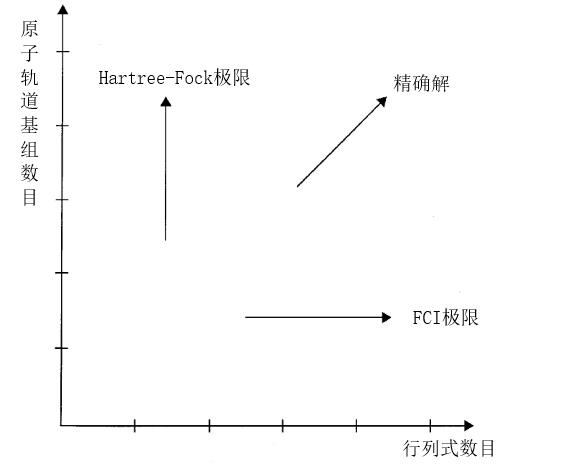
\includegraphics[width = 9cm]{fig/exactsolution.jpg}\\
            \caption{\textbf{量子化学的精确解}}
            \label{exact solution}
          \end{figure}
          
          这两点经常用Figure \ref{exact solution}这个图来表示。如果只使用一个组态,也就是之后会讲到的Hartree-Fock近似下,不断地增大原子轨道基组的数目,这个极限称为单电子极限,或者Hartree-Fock极限;而在原子轨道大小固定之后,不断增大所使用的组态的个数,最后引入所有的组态就称为FCI极限。同时满足Hartree-Fock极限和FCI极限的计算结果,就是精确解。
          
          尽管计算机已经非常发达,但是实际操作中,第一条暂时不可能实现,当原子轨道基组很大的时候,第二条也很难实现\sout{,好惨啊!}。因此量子化学的精确解,FCI的计算几乎只能适用于非常小的体系\footnote{但是没有那么小,现在已经可以在一个相当大的原子轨道基组的前提下求解$\text{F}_2$的FCI结果。},但很多时候我们对精度的要求并没有这么高。电子结构的发展,就是引入一系列近似方法,为了用尽可能小的计算量,实现尽可能高的计算精度,来满足各种需求。
      \section{Hartree-Fock近似}
        Hartree-Fock近似是量子化学的基础和开端,一旦涉及到使用Hartree理论或Hartree-Fock理论计算单分子(非固体)的问题,就已经进入到了量子化学的领域。同时,几乎所有更高精度的电子结构方法都是以HF方法为基础,或者直接从HF方法的结果出发的,因此HF方法的正确理解关系到整个电子结构理论框架的理解。在各种教材中,讲解HF理论的方法有很多种,鉴于电子结构方法前后的完整性,我们选用了其中一种,一个很重要的特殊之处在于我们尽可能使用量子化学家的语言,并且跳过了Hartree理论。这样的写法可能会比较难,因此我们第一小节给出了一个类似结论性质的总结,再在后面几个小节中给出它的来源,以防止读者被数学推导淹没而忘记了我们的目的。
        
        我们在电子结构的后面每一节中都会有这样的小节,这些内容相对较难,而且如果不涉及电子结构理论的话,并不会经常用到,因此各位可以按需跳过它们,但是编者建议对电子结构方法感兴趣的读者或者\sout{或者背上电子结构的锅的}读者认真阅读这些小节,毕竟这些都是电子结构理论的基础内容,在相关书籍中和文献中会多次用到。
        
        读者若发现本指南的逻辑与一些书籍相左,请根据各自的框架理解。
        \subsection{HF方法概论}
          上一节中我们已经给出了量子化学的精确解和目前最精确的计算方法,但是我们也提到,FCI方法由于对计算量和内存的巨大需求几乎不可能作为一个普适方法。因此多少年来,量子化学家们一直在寻找合适的\sch 方程的近似解。其中最经典的,就是Hartree-Fock近似。

          这个近似非常平凡,就是只使用一个Slater行列式表述体系。描述$N$电子体系的最简单的反对称波函数就是只用一个Slater行列式
          \begin{equation}
            | \Psi_{0} \rangle=| \chi_{1} \chi_{2} \cdots \chi_{N} \rangle
            \label{HF gs}
          \end{equation}
          根据变分原理,满足这个函数形式的最好的波函数就是能给出最小的能量期望值的函数,这个能量期望值定义为
          \begin{equation}
            E_{0}=\left\langle\Psi_{0}|\mathscr{H}| \Psi_{0}\right\rangle
            \label{HF energy}
          \end{equation}
          其中$\mathscr{H}$是全电子的哈密顿量,而Slater行列式用自旋轨道展开的方法是唯一的,所以上述变分中可变的部分就是自旋轨道的选择。换句话说,HF方法的核心就在于,如何优化一组自旋轨道$\left\{\chi_1,\chi_2,\dots,\chi_N\right\}$,使得由他们构成的Slater行列式(\ref{HF gs})给出最小的能量期望值。

          这之后的几节将会给出,解决这个问题等价于求解一个本征值问题
          \begin{equation}
            \hat{f}(\mathbf{x}_i)\chi_a(\mathbf{x}_i) = \varepsilon_a\chi_a(\mathbf{x}_i)
            \label{HF equation}
          \end{equation}
          其中$f(i)$称为Fock算符,它的形式为
          \begin{equation}
            f(i)=-\frac{1}{2} \nabla_{i}^{2}-\sum_{A=1}^{M} \frac{Z_{A}}{r_{i A}}+v^{\mathrm{HF}}(i)
          \end{equation}
          其中$v^{\mathrm{HF}}(i)$是把电子和电子之间的相互作用处理成了一个等效的平均势能的形式,通常也称为平均场近似,它的形式将会在后面几节中给出严格定义。
          
          另外,这个平均势能也可以说是第$i$个电子所感受到的“场”,它的大小其实取决于其他电子的自旋轨道,这是一个令人头大的问题,即Fock算符的形式取决于它的本征函数。因此Hartree-Fock方程(\ref{HF equation})是一个非线性方程,没法简单解出结果,只能用迭代的方法求解。这个迭代求解Hartree-Fock方程的步骤称为自洽场(Self-Cosistent-Field, SCF)方法。

          自洽场方法的基本思想是很简单的,只需要先对自旋轨道有一个初始猜测,就可以计算出每个电子感受到的势能,也就是有了Fock算符的形式,然后就可以解本征值方程(\ref{HF equation}) 得到一组新的自旋轨道。用这组新的自旋轨道,就可以得到新的势能,新的Fock算符,又能得到新的自旋轨道,不断重复这个过程直到完成自洽(计算得到的势能不再变化,前后两次的本征函数相同)。
          
          求解这个本征值问题一般需要一组基函数,基函数组$\left\{\phi_i\right\}$越大越完备,自旋轨道展开的可变自由度就越大,能量的期待值(\ref{HF energy})就越小。越来越大的基组将会把Hartree-Fock能量$E_0$越降越低,直到达到一个极限,即上节提到的Hartree-Fock 极限。

          另外,HF近似有时候又被称作单电子近似,但这不意味着HF基态波函数(\ref{HF gs})是一个单电子波函数。所谓单电子近似只是说求解HF方程时,Fock算符只包含了一个电子的信息,电子之间的相互作用变成了平均场,所有电子是等价的,得到的本征值也是单电子的自旋轨道,或者消去自旋部分就是分子轨道。
          
          很多时候,由于化学图像清晰,人们经常使用分子轨道来讨论问题,这与后文中提到的Koopmans定理是有密切联系的。但是需要提醒读者的是,分子轨道(单电子轨道)不是量子化学的目的,它只是用于构建多电子波函数的基础。而HF方法的逻辑,也需要注意,并不是优化单电子自旋轨道的能量,而是优化能量最低的$N$个单电子自旋轨道构成的那个多电子波函数(Slater行列式)的能量,尽管很多时候这两者是等价的。

          在推导Hartree-Fock方程之前,我们需要其他的一些基础内容,接下来的几小节内我们将慢慢道来。
          
        \subsection{单行列式的能量}
          我们首先讨论一个问题,我们如果知道一个N电子的Slater行列式,它由自旋轨道组$\left\{\chi_1, \chi_2,\dots,\chi_N\right\}$构成,那么它的能量期望值是多少?同样,为了回答这个问题,我们先考虑一个简单的情况,就是两电子问题,读者可以把它想象成$\text{H}_2$中的两个电子,描述这个两电子的波函数是一个二阶的Slater行列式
          \begin{equation}
            |\Psi\rangle = |\chi_1 \chi_2\rangle=2^{-1 / 2}\left(\chi_{1}\left(\mathbf{x}_{1}\right) \chi_{2}\left(\mathbf{x}_{2}\right)-\chi_{2}\left(\mathbf{x}_{1}\right) \chi_{1}\left(\mathbf{x}_{2}\right)\right)
          \end{equation}
          描述两电子体系的,略去原子核之间斥力的BO近似下的哈密顿量为
          \begin{equation}
            \begin{aligned} \mathscr{H} &=\left(-\frac{1}{2} \nabla_{1}^{2}-\sum_{A} \frac{Z_{A}}{r_{1 A}}\right)+\left(-\frac{1}{2} \nabla_{2}^{2}-\sum_{A} \frac{Z_{A}}{r_{2 A}}\right)+\frac{1}{r_{12}} \\ &=h(1)+h(2)+\frac{1}{r_{12}} \end{aligned}
          \end{equation}
          按照上式的写法,我们用$h(i)$表示只含有第$i$个电子的哈密顿量,通常称为单电子部分。而$\frac{1}{r_{12}}$就是双电子部分。我们分别计算这些项的期望值,首先对$h(1)$我们有
          \begin{equation}
            \begin{aligned}
              \left\langle\Psi|h(1)| \Psi \right\rangle=\int &\mathrm{d} \mathbf{x}_{1} \mathrm{d} \mathbf{x}_{2} \{ \left[2^{-1 / 2}\left(\chi_{1}\left(\mathbf{x}_{1}\right) \chi_{2}\left(\mathbf{x}_{2}\right)-\chi_{2}\left(\mathbf{x}_{1}\right) \chi_{1}\left(\mathbf{x}_{2}\right)\right)\right]^{*} \\ 
              \times& h\left(\mathbf{r}_{1}\right)\left[2^{-1 / 2}\left(\chi_{1}\left(\mathbf{x}_{1}\right) \chi_{2}\left(\mathbf{x}_{2}\right)-\chi_{2}\left(\mathbf{x}_{1}\right) \chi_{1}\left(\mathbf{x}_{2}\right)\right)\right] \} \\
              =\frac{1}{2} \int \mathrm{d} \mathbf{x}_{1} \mathrm{d} \mathbf{x}_{2} [\chi_{1}^{*}\left(\mathbf{x}_{1}\right) \chi_{2}^{*}\left(\mathbf{x}_{2}\right) h\left(\mathbf{r}_{1}\right) &\chi_{1}\left(\mathbf{x}_{1}\right) \chi_{2}\left(\mathbf{x}_{2}\right)+\chi_{2}^{*}\left(\mathbf{x}_{1}\right) \chi_{1}^{*}\left(\mathbf{x}_{2}\right) h\left(\mathbf{r}_{1}\right) \chi_{2}\left(\mathbf{x}_{1}\right) \chi_{1}\left(\mathbf{x}_{2}\right)\\
              -\chi_{1}^{*}\left(\mathbf{x}_{1}\right) \chi_{2}^{*}\left(\mathbf{x}_{2}\right) h\left(\mathbf{r}_{1}\right) \chi_{2}\left(\mathbf{x}_{1}\right) &\chi_{1}\left(\mathbf{x}_{2}\right)-\chi_{2}^{*}\left(\mathbf{x}_{1}\right) \chi_{1}^{*}\left(\mathbf{x}_{2}\right) h\left(\mathbf{r}_{1}\right) \chi_{1}\left(\mathbf{x}_{1}\right) \chi_{2}\left(\mathbf{x}_{2}\right) ]
            \end{aligned}
          \end{equation}
          读者不要被上式的长度吓到,只是一个展开而已,而且由于我们研究的是第一个电子,因此关于$\mathbf{x}_2$的积分可以直接积掉,这样后两项就由于自旋轨道的正交归一性直接等于零。前两项也只剩下对$\mathbf{x}_1$的积分,即
          \begin{equation}
            \left\langle\Psi_{0}|h(1)| \Psi_{0}\right\rangle=\frac{1}{2} \int \mathrm{d} \mathbf{x}_{1} \chi_{1}^{*}\left(\mathbf{x}_{1}\right) h\left(\mathbf{r}_{1}\right) \chi_{1}\left(\mathbf{x}_{1}\right)+\frac{1}{2} \int \mathrm{d} \mathbf{x}_{1} \chi_{2}^{*}\left(\mathbf{x}_{1}\right) h\left(\mathbf{r}_{1}\right) \chi_{2}\left(\mathbf{x}_{1}\right)
          \end{equation}
          由于积分指标为哑指标,我们计算第二个单电子部分就会发现$\left\langle\Psi_{0}|h(2)| \Psi_{0}\right\rangle=\left\langle\Psi_{0}|h(1)| \Psi_{0}\right\rangle$,因此
          \begin{equation}
            \left\langle\Psi\left|h\left(\mathbf{r}_{1}\right) + h\left(\mathbf{r}_{2}\right)\right| \Psi\right\rangle=\int \mathrm{d} \mathbf{x}_{1} \chi_{1}^{*}\left(\mathbf{x}_{1}\right) h\left(\mathbf{r}_{1}\right) \chi_{1}\left(\mathbf{x}_{1}\right)+\int \mathrm{d} \mathbf{x}_{1} \chi_{2}^{*}\left(\mathbf{x}_{1}\right) h\left(\mathbf{r}_{1}\right) \chi_{2}\left(\mathbf{x}_{1}\right)
          \end{equation}
          我们引入一种简写的记号来标记单电子积分
          \begin{equation}
            [i|h| j]=\langle i|h| j\rangle\equiv \int \mathrm{d} \mathbf{x}_{1} \chi_{i}^{*}\left(\mathbf{x}_{1}\right) h\left(\mathbf{r}_{1}\right) \chi_{j}\left(\mathbf{x}_{1}\right)
            \label{single electron integral}
          \end{equation}
          哈密顿量的单电子部分可以被简写成
          \begin{equation}
            \left\langle\Psi\left|h\left(\mathbf{r}_{1}\right) + h\left(\mathbf{r}_{2}\right)\right| \Psi\right\rangle=\sum_{i=1}^{2}[i|h|i]
          \end{equation}

          接下来计算双电子部分,又是一个很长的公式
          \begin{equation}
            \begin{aligned}
              \langle\Psi|\frac{1}{r_{12}}| \Psi \rangle=\int &\mathrm{d} \mathbf{x}_{1} \mathrm{d} \mathbf{x}_{2} \{ \left[2^{-1 / 2}\left(\chi_{1}\left(\mathbf{x}_{1}\right) \chi_{2}\left(\mathbf{x}_{2}\right)-\chi_{2}\left(\mathbf{x}_{1}\right) \chi_{1}\left(\mathbf{x}_{2}\right)\right)\right]^{*} \\ 
              \times& \frac{1}{r_{12}}\left[2^{-1 / 2}\left(\chi_{1}\left(\mathbf{x}_{1}\right) \chi_{2}\left(\mathbf{x}_{2}\right)-\chi_{2}\left(\mathbf{x}_{1}\right) \chi_{1}\left(\mathbf{x}_{2}\right)\right)\right] \} \\
              =\frac{1}{2} \int \mathrm{d} \mathbf{x}_{1} \mathrm{d} \mathbf{x}_{2} [\chi_{1}^{*}\left(\mathbf{x}_{1}\right) \chi_{2}^{*}\left(\mathbf{x}_{2}\right) \frac{1}{r_{12}}&\chi_{1}\left(\mathbf{x}_{1}\right) \chi_{2}\left(\mathbf{x}_{2}\right)+\chi_{2}^{*}\left(\mathbf{x}_{1}\right) \chi_{1}^{*}\left(\mathbf{x}_{2}\right) \frac{1}{r_{12}} \chi_{2}\left(\mathbf{x}_{1}\right) \chi_{1}\left(\mathbf{x}_{2}\right)\\
              -\chi_{1}^{*}\left(\mathbf{x}_{1}\right) \chi_{2}^{*}\left(\mathbf{x}_{2}\right) \frac{1}{r_{12}} \chi_{2}\left(\mathbf{x}_{1}\right) &\chi_{1}\left(\mathbf{x}_{2}\right)-\chi_{2}^{*}\left(\mathbf{x}_{1}\right) \chi_{1}^{*}\left(\mathbf{x}_{2}\right) \frac{1}{r_{12}} \chi_{1}\left(\mathbf{x}_{1}\right) \chi_{2}\left(\mathbf{x}_{2}\right) ]
            \end{aligned}
          \end{equation}
          因为积分指标都是哑指标,所以我们发现,第一项和第二项相等,第三项和第四项相等
          \begin{equation}
            \begin{aligned}\langle\Psi| \frac{1}{r_{12}} | \Psi\rangle=& \int \mathrm{d} \mathbf{x}_{1} \mathrm{d} \mathbf{x}_{2} \chi_{1}^{*}\left(\mathbf{x}_{1}\right) \chi_{2}^{*}\left(\mathbf{x}_{2}\right) r_{12}^{-1} \chi_{1}\left(\mathbf{x}_{1}\right) \chi_{2}\left(\mathbf{x}_{2}\right) \\ &-\int \mathrm{d} \mathbf{x}_{1} \mathrm{d} \mathbf{x}_{2} \chi_{1}^{*}\left(\mathbf{x}_{1}\right) \chi_{2}^{*}\left(\mathbf{x}_{2}\right) r_{12}^{-1} \chi_{2}\left(\mathbf{x}_{1}\right) \chi_{1}\left(\mathbf{x}_{2}\right) \end{aligned}
          \end{equation}
          如果我们引入另一种记号,来简记双电子积分
          \begin{equation}
            [i j | k l] =\left[\chi_{i} \chi_{j} | \chi_{k} \chi_{l}\right]\equiv\int \mathrm{d} \mathbf{x}_{1} \mathrm{d} \mathbf{x}_{2} \chi_{i}^{*}\left(\mathbf{x}_{1}\right) \chi_{j}\left(\mathbf{x}_{1}\right) r_{12}^{-1} \chi_{{k}}^{*}\left(\mathbf{x}_{2}\right) \chi_{l}\left(\mathbf{x}_{2}\right)
            \label{double electron integral}
          \end{equation}
          需要注意,上式定义中,调整了波函数的位置,算符左边写第一个电子的波函数,右边是第二个电子的波函数,带星的自旋轨道在不带星的左边。如果自旋轨道都是实的,这在多数条件下都是成立的,只要你不涉及平面波基组或者相对论量子化学,显然上述定义满足如下的对称性
          \begin{equation}
            [i j | k l]=[j i | k l]=[i j | l k]=[j i | l k]
          \end{equation}
          原本的哈密顿量双电子部分就可以写作
          \begin{equation}
            \langle\Psi|\frac{1}{r_{12}}| \Psi \rangle = [11|22] - [12|21]
          \end{equation}
          
          经过这么一大堆折腾,我们终于回答了最初问题的一个最简单的版本,即对于一个两电子体系,一个由$\chi_1, \chi_2$构成的Slater行列式的能量期望值为
          \begin{equation}
            \langle \Psi|\mathscr{H}|\Psi\rangle = [1|h|1] + [2|h|2] + [11|22] - [12|21]
          \end{equation}
          但是从两电子往多电子的推广是平凡的,对于一个$N$电子的体系,由$\chi_1, \chi_2,\dots,\chi_N$构成的Slater行列式的能量期望值为
          \begin{equation}
            \langle \Psi|\mathscr{H}|\Psi\rangle =\sum_{m=1}^N [m|h|m] + \sum_{m=1}^N\sum_{n>m}^N \left([mm|nn] - [mn|nm]\right)
          \end{equation}
          根据双电子积分简记符号的定义(\ref{double electron integral})和积分哑指标的特性,容易发现$[mm|nn] = [nn|mm]$和$[mn|nm]=[nm|mn]$,而且当$m=n$时,$[mm|nn] - [mn|nm] = 0$,这三条允许我们去掉求和中的限制条件($n>m$),只需要在前面加一个$1/2$,对于一个$N$电子的Slater行列式,它的能量期望值我们最终可以写成
          \begin{equation}
            \langle \Psi|\mathscr{H}|\Psi\rangle =\sum_{m=1}^N [m|h|m] + \frac{1}{2}\sum_{m=1}^N\sum_{n=1}^N \left([mm|nn] - [mn|nm]\right)
          \end{equation}
          上述$N$电子Slater行列式的结果读者可自行推导,与两电子情况差别并不大,核心点在于把跟积分无关的自由度都积分积掉,这样就只剩下了一个两电子问题,可以参照文献\cite{Szabo1989Modern}的2.3.4节。
        \subsection{单行列式能量期望的变分}
          按照Hartree-Fock方法的逻辑,我们期望找到一组更好的自旋轨道,使得这组自旋轨道构成的行列式能量最低。这是一种泛函的思想,即从函数形式(自旋轨道)到数(能量)的映射,我们需要变分的思想,这与微积分中学到的极值问题是一样的,我们期望寻找一个函数形式变化的极小值,也就是能量关于自旋轨道的变分等于零的那个点,对应着函数的导数等于零的极值点。

          但是自旋轨道的形式也不能随便变化,比如说它们不管怎么变都要满足正交归一的要求,因此我们要求解的是一个限制条件下的变分。在微积分中,我们求条件极值的方法是拉格朗日乘子法,在变分的框架下也是一样的。我们的限制条件为
          \begin{equation}
            \int \mathrm{d} \mathbf{x}_{1} \chi_{a}^{*}(\mathbf{x}_{1}) \chi_{b}(\mathbf{x}_{1})=[a | b]=\delta_{a b}
          \end{equation}
          所以我们关于自旋轨道的“拉格朗日乘子法”的泛函形式为
          \begin{equation}
            \mathscr{L}\left[\left\{\chi_{a}\right\}\right]=E_{0}\left[\left\{\chi_{a}\right\}\right]-\sum_{a=1}^{N} \sum_{b=1}^{N} \varepsilon_{b a}\left([a | b]-\delta_{a b}\right)
            \label{Lagrange functional}
          \end{equation}
          其中$\varepsilon_{b a}$为拉格朗日乘子,如果我们假定整个泛函为实数,由于$[a | b]=[b | a]^{*}$,所有的拉格朗日乘子必须满足厄米性$\varepsilon_{b a}=\varepsilon_{a b}^{*}$。$E_0$就是单行列式的能量期望值,根据上一节的结论,它的形式为
          \begin{equation}
            E_{\mathrm{o}}\left[\left\{\chi_{a}\right\}\right]=\sum_{a=1}^{N}[a|h| a]+\frac{1}{2} \sum_{a=1}^{N} \sum_{b=1}^{N}[a a | b b]-[a b | b a]
          \end{equation}
          当自旋轨道的形式变化一点点,即$\chi_{a} \rightarrow \chi_{a}+\delta \chi_{a}$时,要想满足限制条件下的能量最小,泛函(\ref{Lagrange functional})的变分必须为零,
          \begin{equation}
            \delta \mathscr{L}=\delta E_{0}-\sum_{a=1}^{N} \sum_{b=1}^{N} \varepsilon_{b a} \delta[a | b]=0
          \end{equation}
          变分与求导类似,上述等式的两个部分可以分别写作
          \begin{equation}
            \delta[a | b]=\left[\delta \chi_{a} | \chi_{b}\right]+\left[\chi_{a} | \delta \chi_{b}\right]
            \label{overlap variation}
          \end{equation}
          \begin{equation}
            \begin{aligned}
              \delta E_{0}=&\sum_{a=1}^{N}\left[\delta \chi_{a}|h| \chi_{a}\right]+\left[\chi_{a}|h| \delta \chi_{a}\right]\\
              &+\frac{1}{2} \sum_{a=1}^{N} \sum_{b=1}^{N}\left[\delta \chi_{a} \chi_{a} | \chi_{b} \chi_{b}\right]+\left[\chi_{a} \delta \chi_{a} | \chi_{b} \chi_{b}\right]+\left[\chi_{a} \chi_{a} | \delta \chi_{b} \chi_{b}\right]+\left[\chi_{a} \chi_{a} | \chi_{b} \delta{\chi_b}\right]\\
              &-\frac{1}{2} \sum_{a=1}^{N} \sum_{b=1}^{N}\left[\delta \chi_{a} \chi_{b} | \chi_{b} \chi_{a}\right]+\left[\chi_{a} \delta \chi_{b} | \chi_{b} \chi_{a}\right]+\left[\chi_{a} \chi_{b} | \delta \chi_{b} \chi_{a}\right]+\left[\chi_{a} \chi_{b} | \chi_{b} \delta \chi_a \right]
            \end{aligned}
            \label{energy variation}
          \end{equation}
          首先看等式(\ref{overlap variation}),根据这种单电子积分符号的定义(\ref{single electron integral}),容易看出第二项是第一项的复共轭。类似的,在等式(\ref{energy variation})中,根据单电子算符和双电子算符的厄米性,第一行的两项互为复共轭,第二和第三行中,第一项和第二项互为复共轭,第三项和第四项分别互为复共轭。不但如此,第二行和第三行中,由于积分指标是哑指标可以交换,因此第一项和第三项相等,第二项和第四项相等,这可以帮助我们消去前面的$1/2$。这样一来,原本的变分的形式就被大大简化了,变为
          \begin{equation}
            \begin{aligned}
              \delta \mathscr{L}=&\sum_{a=1}^{N}\left[\delta \chi_{a}|h| \chi_{a}\right]+\sum_{a=1}^{N} \sum_{b=1}^{N}\left[\delta \chi_{a} \chi_{a} | \chi_{b} \chi_{b}\right]-\left[\delta \chi_{a} \chi_{b} | \chi_{b} \chi_{a}\right]\\
              &-\sum_{a=1}^{N} \sum_{b=1}^{N} \varepsilon_{b a}\left[\delta \chi_{a} | \chi_{b}\right]+\text{复共轭} = 0
            \end{aligned}
          \end{equation}
          一个数加上自己的复共轭为零,说明它是一个纯虚数或者零,因为我们假定了这个泛函是实数,因此只需要让前一部分等于零。希望读者没有忘记我们引入简化积分的记号,我们将复共轭之前的部分的完全体写出来
          \begin{equation}
            \begin{aligned}
              \sum_{a=1}^{N} \int \mathrm{d} \mathbf{x}_{1} \delta \chi_{a}^{*}(1)\left\{h(1) \chi_{a}(1)+\sum_{b=1}^{N}\left[\left(\int \mathrm{d} \mathbf{x}_{2} \chi_{b}^{*}(2) r_{12}^{-1} \chi_{b}(2)\right) \chi_{a}(1)-\right.\right. \\ 
              \left.\left. \left(\int \mathrm{d} \mathbf{x}_{2} \chi_{b}^{*}(2) r_{12}^{-1} \chi_{a}(2)\right) \chi_{b}(1)\right] -\sum_{b=1}^{N} \varepsilon_{b a} \chi_{b}(1)\right\} = 0
            \end{aligned}
          \end{equation}
          由于变分是任意的,所以上式大括号中的部分等于零,稍作整理我们就能写出变分推导的结果:
          \begin{equation}
            \begin{aligned}
              h(1) \chi_{a}(1)+\sum_{b=1}^{N}\left[\left(\int \mathrm{d} \mathbf{x}_{2} \chi_{b}^{*}(2) r_{12}^{-1} \chi_{b}(2)\right) \chi_{a}(1)-\right. \\ 
              \left. \left(\int \mathrm{d} \mathbf{x}_{2} \chi_{b}^{*}(2) r_{12}^{-1} \chi_{a}(2)\right) \chi_{b}(1)\right] =\sum_{b=1}^{N} \varepsilon_{b a} \chi_{b}(1)
            \end{aligned}
            \label{HF GS energy variation}
          \end{equation}
        \subsection{库伦算符、交换算符和Fock算符}
          我想读者也觉得上一节中最后的式子比较复杂,关键是比较长,所以人们期望引入一些记号才简化书写,有些时候,这些简化的标记也是有物理意义的。我们在这一节将引入两个新算符,并且用它们简化等式(\ref{HF GS energy variation})最后得到Hartree-Fock方程和Fock算符。
          
          我们是通过它们对自旋轨道的作用来定义这两个新算符的,首先是库伦算符,它通常用字母$J$或者它的花体表示
          \begin{equation}
            \mathscr{J}_{b}(1) \chi_{a}(1)=\left[\int \mathrm{d} \mathbf{x}_{2} \chi_{b}^{*}(2) r_{12}^{-1} \chi_{b}(2)\right] \chi_{a}(1)
            \label{Coulomb operator}
          \end{equation}
          它的形式非常像一个简单的库伦相互作用,读者仔细看就会发现这就是式(\ref{HF GS energy variation})中括号内对$b$求和的第一项。我们同样希望简单求和的第二项,它的形式没有那么平凡,这是因为它的出现来源于Slater行列式的交换反对称性。我们引入交换算符,它通常用字母$K$或者它的花体表示
          \begin{equation}
            \begin{aligned} \mathscr{K}_{b}(1) \chi_{a}(1) &=\left[\int \mathrm{d} \mathbf{x}_{2} \chi_{b}^{*}(2) r_{12}^{-1} \chi_{a}(2)\right] \chi_{b}(1) \\ &=\left[\int \mathrm{d} \mathbf{x}_{2} \chi_{b}^{*}(2) r_{12}^{-1} \mathscr{P}_{12} \chi_{b}(2)\right] \chi_{a}(1) \end{aligned}
            \label{Exchange operator}
          \end{equation}
          为了简化,我们\sout{不择手段地}使用了$\mathscr{P}_{12}$,它能交换1电子和2电子的位置。如此一来,我们就可以将等式(\ref{HF GS energy variation})简化成一个写起来比较简单的形式
          \begin{equation}
            \left[h(1)+\sum_{b=1}^{N} \mathscr{J}_{b}(1)-\mathscr{K}_{b}(1)\right] \chi_{a}(1)=\sum_{b=1}^{N} \varepsilon_{b a} \chi_{b}(1)
          \end{equation}
          再进一步,我们定义Fock算符
          \begin{equation}
            \hat{f} = h(1)+\sum_{b=1}^{N} \mathscr{J}_{b}(1)-\mathscr{K}_{b}(1)
            \label{Fock operator}
          \end{equation}
          这样就得到了一个看上去非常简单的形式
          \begin{equation}
            \hat{f}  \chi_{a} =\sum_{b=1}^{N} \varepsilon_{b a}  \chi_{b} 
            \label{fake HF equation}
          \end{equation}
          这个形式与我们之前给出的Hartree-Fock方程(\ref{HF equation})已经非常相似,只是右侧没有求和。

          熟悉线性代数的读者可以看出,有一个求和号是因为上式中的$\chi_{a}$不是Fock算符的本征态。不出意外地,Fock算符是一个厄米算符,根据复数域上的谱定理,一定可以找到它的一组单位正交的本征态,这样就可以把求和号扔掉了。但是问题在于我们能否做这件事,换句话说,我们利用等式(\ref{fake HF equation})中的$\chi_{a}$线性组合得到的Fock算符的单位正交的本征态,能否仍然保证变分的意义,即组成的行列式能量最低呢?
          
          答案是肯定的。读者可以利用幺正算符的性质证明,将一组正交归一的自旋轨道$\left\{\chi_i\right\}$作幺正变换(线性组合)得到新的一组正交归一自旋轨道$\left\{\chi_i^{\prime}\right\}$,两者构成的行列式的能量期望值是相等的,即
          \begin{equation}
            \langle\chi_1\chi_2\cdots\chi_N|\mathscr{H}|\chi_1\chi_2\cdots\chi_N\rangle = \langle\chi_1^{\prime}\chi_2^{\prime}\cdots\chi_N^{\prime}|\mathscr{H}|\chi_1^{\prime}\chi_2^{\prime}\cdots\chi_N^{\prime}\rangle
          \end{equation}
          所以我们可以利用等式(\ref{Fock operator})中的Fock算符的本征态作为自旋轨道,这样构成的Slater行列式仍然是能量最低的。这样Hartree-Fock方法的推导就结束了,最终得到了一个我们在第一节中就提出的只关于单电子轨道的本征值问题
          \begin{equation}
            \hat{f}(\mathbf{x}_i)\chi_a^{\prime}(\mathbf{x}_i) = \varepsilon_a\chi_a^{\prime}(\mathbf{x}_i)
          \end{equation}
          此时的Hartree-Fock方程通常被称为Hartree-Fock方程的正则(标准)形式,解得的本征态也称为正则自旋轨道,此后如果再用到这个等式,我们将把撇去掉。当然正如我们在第一节所说的那样,这个本征值问题是非线性问题,只能通过所谓自洽场的方法求解。
        \subsection{非正交基组的本征值问题}
          上一小节我们知道,求单Slater行列式的最小能量等价于求解Fock算符的本征值问题,通常在数学上,本征值问题的“基组”都是正交的这是因为数学上空间的单位正交基其实是让一个分量为1其他分量为0的矢量。但是在量子化学中,原子轨道基组并不正交,一个H原子的1s轨道和相邻C原子的1s轨道内积并不是零。所以本征值问题会稍微有点变化,我们在这里提出这个问题,一方面是导出Hartree-Fock近似下最后真正求解的“久期方程”\footnote{编者认为,在我们的逻辑框架下,HF的久期方程并不是通过线性变分法(在组态相关一节中会介绍)导出的,这是因为我们的逻辑并不是变分优化分子轨道的能量,而是优化行列式的能量,虽然这两者是等价的},同时也想提醒读者,这个不正交的特性经常被忘掉,\sout{导致编者debug了一个月。}

          我们先定义原子轨道基组$\left\{\phi_i\right\}$,他们之间不满足正交归一性,而是存在一个重叠积分矩阵
          \begin{equation}
            {S}_{ij} \equiv \langle \phi_i|\phi_j\rangle = \int \mathrm{d} \mathbf{x} \phi_i^*(\mathbf{x})\phi_j(\mathbf{x})
          \end{equation}
          Fock算符的本征态可以在这个基下展开(我们先忽略自旋的问题,或者认为上述原子轨道其实是自旋轨道),
          \begin{equation}
            |\psi_i\rangle = \sum_j C_{ji} |\phi_i\rangle
          \end{equation}
          这样,系数矩阵$C_{ji} $的第$i$列表示第$i$个分子轨道对原子轨道的展开系数,这与多数软件中的设定是一致的。原本的Fock算符的本征值问题可以写作
          \begin{equation}
            \hat{f}|\psi_j\rangle = \varepsilon_j |\psi_j\rangle
          \end{equation}
          左乘一个$\langle \psi_i|$然后将原子轨道展开代入
          \begin{equation}
            \sum_k\sum_l C_{ki}^* C_{lj} \langle \phi_k|\hat{f}|\phi_l\rangle = \sum_k\sum_l C_{ki}^* C_{lj} \langle \phi_k|\phi_l\rangle \varepsilon_j 
          \end{equation}
          我们定义原子轨道基组下的Fock算符的矩阵为$F_{kl} \equiv \phi_k|\hat{f}|\phi_l$,在很多文献中,这个矩阵称为Fock矩阵。改写上式为
          \begin{equation}
            \sum_k\sum_l C_{ik}^{\dagger} F_{kl} C_{lj} = \sum_k\sum_l  C_{ik}^{\dagger} S_{kl} C_{lj}\varepsilon_j 
          \end{equation}
          即
          \begin{equation}
            \left( C^{\dagger}FC \right)_{ij} = \left( C^{\dagger}SC \varepsilon\right)_{ij}
          \end{equation}
          其中$\varepsilon$为对角线为原本本征能量的对角阵,将上式的矩阵形式左乘$ C^{\dagger -1}$就得到了Hartree-Fock近似下最后求解的方程
          \begin{equation}
            FC = SC \varepsilon
            \label{matrix form of secular equation}
          \end{equation}
          上式经常用于在已知Hartree-Fock分子轨道能量的情况下反推Fock矩阵(比如你有Gaussian计算结果,想知道Fock矩阵的时候),即使用$F = SC \varepsilon C^{-1}$。另外,上式其实是一个矩阵的形式,并不是常见的本征值方程,如果单独拿出某一列,才会化成一般的本征值问题,即
          \begin{equation}
            Fc = ESc
          \end{equation}
          此时$E$只是一个常数,$c$也只是一个列矢量而非之前的矩阵,求解上述本征值问题所用的行列式方程为
          \begin{equation}
            \det\left[F - ES\right] = 0
            \label{secular equation}
          \end{equation}
          上式又被称为久期方程。如果读者熟悉HMO理论,可能会对它感到眼熟,因为HMO中求解的那个行列式就是上式在共轭多烯体系的一个应用,前提是引入一系列的近似,即重要的分子轨道只是由原子轨道中的$p_z$轨道贡献,并且只有邻近原子的$p_z$轨道之间不正交,重叠积分为$\beta$,Fock矩阵也只有对角元$\alpha$,如果把$E$写成$x$,等式(\ref{secular equation})就变成了HMO理论中的行列式方程。

          但是读者应该也发现了,如果有$K$个空间原子轨道,求解方程(\ref{secular equation}),会得到$2K$个自旋轨道,Hartree-Fock近似所使用的其实是由能量最低的$N$个自旋轨道构成的Slater行列式,称为Hartree-Fock基态。在Hartree-Fock基态中被占据的自旋轨道称为占据轨道,未占据的轨道称为未占据轨道,或者另一个常见的名字,虚轨道(Virtual Orbital)。
          
          可以看到,求解久期方程只涉及一个电子的信息,其他的电子的作用变成了一个平均的形式,这某种程度上说的确是一个近似,但我们的推导中似乎没有提及这一个近似,这是为什么呢?如果读者看过Hartree理论的推导就会发现,它必须在某一步将求和中的$i\neq j$删去变成纯粹的对$i$求和,但是Hartree-Fock近似下,这一点是不需要的,因为在能量求和中,当$i=j$时,库仑积分和交换积分抵消了:$[ii|jj] - [ij|ji] = 0$(前提当然是你能接受两个无穷大相减这个操作的话)。这一点也是我们跳过了Hartree理论的原因,编者期望能给读者一个更深的印象,那就是Hartree-Fock的核心近似是\textbf{只用一个Slater行列式描述$N$电子波函数。}鉴于无穷大的问题仍然存在,因此这仍然是一个近似,即单电子近似/平均场近似,电子与电子的运动是不关联的。

          体系的真实能量,或者说FCI解得的能量$\varepsilon_{exact}$与Hartree-Fock基态能量$E_0$之间的差通常被称为电子的关联能,这个值越大,电子的关联也就越强,post-Hartree-Fock方法和后来的DFT理论中,都是试图添加电子之间的关联,只是方法不同。
        \subsection{Hartree-Fock轨道能量与Koopmans定理}
          Hartree-Fock方法远没有读者想的那么平凡和简单,我们在这一小节的开头提一个简单的问题,这一小节就是要回到这个问题:如果Hartree-Fock的Slater行列式由能量最低的$N$个自旋轨道构成,每个自旋轨道占据一个电子,那么Hartree-Fock的基态能量是不是就是这$N$个自旋轨道对应的Fock算符的本征值之和呢?这个问题不能简单套用之前Hartree积的结论,这是因为我们从来没证明过体系总的哈密顿量可以写成Fock算符的求和。那如果不是,那这个“轨道能量”还有意义吗?

          我们直接使用数学工具来说明这个问题,先复习一下Fock算符的形式
          \begin{equation}
            \hat{f} = h + \sum_b^N (\mathscr{J}_b - \mathscr{K}_b)
          \end{equation}
          那Hartree-Fock的某个轨道的能量可以写作
          \begin{equation}
            \begin{aligned}
              \varepsilon_i &=  \langle\chi_i|\hat{f}|\chi_i\rangle = \langle\chi_i|h + \sum_b^N (\mathscr{J}_b - \mathscr{K}_b)|\chi_i\rangle\\
              &=[i|h|i] + \sum_b^N([ii|bb] - [ib|bi])
            \end{aligned}
            \label{orbital energy for HF orbitals}
          \end{equation}
          如果我取$i$为某个占据轨道的编号,用$a$表示,那么在上式对$b$求和时有一项是零,即
          \begin{equation}
            \varepsilon_a=[a|h|a] + \sum_{b\neq a}^N([aa|bb] - [ab|ba])
            \label{orbital energy for occupied}
          \end{equation}
          
          我们分析一下这个等式的物理意义,对于占据轨道的轨道能量,它等于一个电子在这个轨道上的动能和与原子核的势能,加上它与剩余的$N-1$个电子之间的相互作用,这看上去非常合理。但是如此看来,Hartree-Fock轨道的能量显然不应该是所有占据轨道的Fock算符的本征值的和,因为每计算一个轨道的能量,就会将这个轨道上的电子与所有其他占据轨道上电子之间的相互作用考虑在内,因此简单地求和会导致这部分相互作用重复计算了。数学语言来说,Hartree-Fock基态的真正能量为
          \begin{equation}
            E_0 = \sum_a^N [a|h|a] + \frac{1}{2}\sum_a^N \sum_b^N([aa|bb] - [ab|ba])
          \end{equation}
          而Fock算符的本征值求和为
          \begin{equation}
            \sum_a \varepsilon_a = \sum_a^N [a|h|a] + \sum_a^N \sum_b^N([aa|bb] - [ab|ba])
          \end{equation}
          缺少的二分之一就代表了重复计算的电子间的相互作用。

          接下来回答第二个问题,这个“轨道能量”的意义是什么。在这之前,我们看一个有趣的结果,那就是计算一个未占据的Hartree-Fock轨道的Fock算符本征值,我们取等式(\ref{orbital energy for HF orbitals})中的$i$为某个未占据轨道的编号,用$r$表示,那刚刚等于零的那一项就不存在了,求和中的所有项都会保留,即
          \begin{equation}
            \varepsilon_r=[r|h|r] + \sum_{b}^N([rr|bb] - [rb|br])
            \label{orbital energy for virtual}
          \end{equation}
          对于未占据轨道,它的轨道能量等于一个电子在这个轨道上的动能和与原子核的势能,加上它与原本占据的全部$N$个电子之间的相互作用!这等价于在原本电子都不动的基础上加一个电子到第$r$个轨道,而得到的这个新电子的能量。这引导着我们计算一个这个体系的电子亲和能,定义为体系加上一个电子的基态能量与原本的基态能量的差\footnote{可能差一个符号,读者不要在意},我们假设这个$r$指标恰好是LUMO轨道的标号
          \begin{equation}
            \begin{aligned}
              E_A &= -E_0^{(N)} + E_0^{(N+1)} = -\langle \Psi_0|\mathscr{H}|\Psi_0\rangle + \langle \Psi_0^r|\mathscr{H}|\Psi_0^r\rangle \\
              &=-\sum_a^N [a|h|a] - \frac{1}{2}\sum_a^N \sum_b^N([aa|bb] - [ab|ba]) + \sum_a^{N,r} [a|h|a] + \frac{1}{2}\sum_a^{N,r} \sum_b^{N,r}([aa|bb] - [ab|ba])\\
              &=  [r|h|r]  +  \frac{1}{2}\sum_b^{N}([rr|bb] - [rb|br]) +  \frac{1}{2}\sum_a^{N}([aa|rr] - [ar|ra])\\
              &= [r|h|r] + \sum_b^{N}([rr|bb] - [rb|br]) =\varepsilon_r
            \end{aligned}
          \end{equation}
          可以看到,将一个电子加到原本未占据的$r$轨道上所产生的能量就是原本的非占据轨道$r$的轨道能量。同理,我们可以从一个占据轨道$s$拿走一个电子需要的能量,即离子化的能量
          \begin{equation}
            \begin{aligned}
              E_I &= E_0^{(N)} - E_0^{(N-1)} \\
              &= \sum_a^N [a|h|a] + \frac{1}{2}\sum_a^N \sum_b^N([aa|bb] - [ab|ba]) - \sum_{a\neq s}^{N} [a|h|a] - \frac{1}{2}\sum_{a\neq s}^{N} \sum_{a\neq s}^{N}([aa|bb] - [ab|ba])\\
              &=  [s|h|s]  +  \frac{1}{2}\sum_{b\neq s}^{N}([ss|bb] - [sb|bs]) +  \frac{1}{2}\sum_{a\neq s}^{N}([aa|ss] - [as|sa])\\
              &= [s|h|s] + \sum_{b\neq s}^{N}([ss|bb] - [sb|bs]) =\varepsilon_s
            \end{aligned}
          \end{equation}
          可以看到,从一个已占据轨道$s$上移走一个电子需要的能量就是原本的占据轨道$s$的轨道能量。
          
          以上两个式子也就是Hartree-Fock方法解出的轨道能量的意义,这最早被总结成了一个定理,\textbf{Koopmans定理:在一个给定的$N$电子Hartree-Fock单行列式中,占据轨道$\chi_a$的轨道能量等于从这个轨道上移走一个电子所需要的能量;非占据轨道$\chi_r$的轨道能量等于新加一个在这个轨道上的电子额外引入的能量。}或者换句话说,\textbf{Hartree-Fock近似的HOMO能量基本等于体系的第一电离能,LUMO能量基本等于体系的第一电子亲和能。}\footnote{当然,按照定义应该是差一个正负号。}

          显然,Koopmans定理是一个近似的定理,它基于我们上面的两个推导,而这两个推导是基于一个假设,即增加电子和减少电子时,体系的Hartree-Fock解出的自旋轨道不变。这显然不是什么很好的假设,电子数的多少原则上会影响轨道,严格计算上需要加减电子之后重新计算本征态,再计算电离能和电子亲和能。所以用单电子图像(分子轨道)分析电离能、电子亲和能以及电子跃迁原则上都是一个很大的近似,即使是DFT得到的添加了电子关联的分子轨道。但是,用Hartree-Fock计算得到的中性分子的第一电离能(电子亲和能不行)往往是比较准确的,这是因为一个非常非常凑巧的正负误差的抵消,即加减电子引起的自旋轨道的重排和驰豫的能量恰好与电子关联的能量修正大小相近,符号相反。

      \section{Hartree-Fock方法的数值计算}
        \subsection{基组}
          由于前面所提到的,一个基组使一个偏微分方程求解转换为线性代数的求解,从而使用计算机来进行数值计算这样的电子结构成为了可能。然而,数值计算对数值的稳定性以及精确度的要求相当地高,这可以类比为物理实验中多次测量导致的误差积累,在程序运行过程中由于使用了双精度这样只有有限有效位数的数字,即便是简单的加减乘除也会导致误差逐渐积累,使最后的结果可能完全变了样。因此在这样的科学计算中我们希望能够尽可能保留精确解,使产生误差的来源尽可能减少。这也因此高斯基组在电子结构计算中极其流行——其存在使一些复杂的积分如重叠积分、库伦积分等能够给出精确解,从而极大提高数值稳定性,同时加快运算速度(因为数值积分极其耗时)。

          在实际基组中一个电子轨道往往表示为多个高斯函数的叠加:
          \begin{equation}
            \psi (\boldsymbol{r};\boldsymbol{r}_0,\boldsymbol{a}) \sim \sum_i c_i (x-x_0)^{a_x}(y-y_0)^{a_y}(z-z_0)^{a_z} e^{- \alpha_i (\boldsymbol{r} - \boldsymbol{r}_0)^2}.
          \end{equation}
          因此在实际的理论推导过程中电子轨道积分会转换为一个个高斯函数与算符之间的积分。而复杂的角向函数被转化为了简单的$x,y,z$的幂函数,从而为提供精确解扫除了另一障碍。

          一般的电子结构程序使用的基组套装是从Basis Set Exchange (\url{https://www.basissetexchange.org}) 里面扒下来的,它会告诉你这个shell它会有多少个高斯函数,每个高斯函数的指数和系数分别是多少。

          解决完基组后,我们便可以开始研究那些矩阵的数值表达方式。我们需要解决的是这么一个线性代数(特征值)问题,
            \begin{equation}
                F C = S C E
            \end{equation}
            其中$F$和$S$是我们需要实现求出来的。我们从最简单的$S$开始。

        \subsection{重叠积分}
          定义是这个:
          \begin{equation}
              S_{ij} = \langle \phi_i | \phi_j \rangle = \int \phi_i(\boldsymbol{r}) \phi_j(\boldsymbol{r}) d \boldsymbol{r}.
          \end{equation}
          所幸$\phi_i$和$\phi_j$都是高斯函数(或者乘上一个多项式),而这样的形式是能够给出精确解的,比如下面这个公式:
          \begin{equation}
              \int_\mathrm{R^n}\, dX \, f(X)\,e^{-\frac{1}{2}X^T A X + B^T X }= \sqrt{\frac{(2\pi)^n}{\mathrm{det} A}}e^{\frac{1}{2}B^T A^{-1}B} \mathrm{exp}\left(\frac{1}{2}(A^{-1})_{ij} \frac{\partial}{\partial x_i}\frac{\partial}{\partial x_j}\right) f(X) \bigg|_{X=B}
          \end{equation}
          它表达了对于包括任意数量的自变量$X$以及一个函数(最好是多项式),给出高斯函数的二次项矩阵$A$和一次项矢量$B$的情况下得到的精确解。其中$\exp$部分应理解为
          \begin{equation}
              \exp{\hat{g}} = \sum_n \frac{\hat{g}^n}{n!}
          \end{equation}
          当然这么写程序会非常难(我也只能在擅长符号计算的\emph{Mathematica}里实现它)。所幸电子轨道的样子是非常有规律的,所以我们可以通过 Obara \& Saika 提示的迭代关系来实现。

          我们先展现所使用的符号。对于一个高斯函数,
          \begin{equation}
              |a) \equiv g(\vec{r},\alpha,\boldsymbol{a},\vec{A}) = (x- A_x)^{a_x} (y-A_y)^{a_y} (z-A_z)^{a_z} \exp \left(-\alpha |\vec{r} - \vec{A}|^2\right)
          \end{equation}
          有一个 Gaussian Product Theorem,即\cite{may2006density}:
          \begin{theorem}
              两个高斯函数的乘积可转换为一系列高斯函数的和,比如:
              \begin{equation}
                  g(\vec{r},\alpha, \boldsymbol{0},\vec{A})g(\vec{r},\beta, \boldsymbol{0},\vec{B}) = \exp(-\xi |\overline{AB}|^2) g(\vec{r},\zeta,\boldsymbol{0},\vec{P}),
              \end{equation}
              其中$\zeta = \alpha + \beta, \, \xi = \frac{\alpha\beta}{\zeta}, \, \vec{P} = \frac{\alpha \vec{A} + \beta \vec{B}}{\zeta}, \, \overline{AB} = \vec{A} - \vec{B}$.
              对于含有多项式的高斯函数。可以利用
              \begin{equation}
                  (x- A_x) ^{a_x} = [(x-P_x) + \overline{PA}_x]^{a_x} = \sum_{i=0}^{a_x} C_{a_x}^i (x-P_x)^i {PA}_x^{a_x - i}
              \end{equation}
              从而可以展开两个高斯函数的乘积为
              \begin{equation}
                  g_1g_2 = \exp(-\xi|AB|^2) \exp(-\zeta|\vec{r} - \vec{P}|^2) \times \prod_{k=x,y,z} \sum_{i=0}^{i=a_k+b_k}(k-P_k)^i f_i (a_k,b_k,\overline{PA}_k,\overline{PB}_k),
              \end{equation}
              其中
              \begin{equation}
                  f_i(a_k,b_k,\overline{PA}_k,\overline{PB}_k) = \sum_{n=0}^{n=i} C_{a_k}^{n} C_{b_k}^{i-n} \overline{PA}_k^{a_x-n}\overline{PB}_k^{b_x-n+k}
              \end{equation}
          \end{theorem}
          但这不迭代啊!
          
          高斯函数还有一个特殊的性质,我们可以通过对它进行求导来得到一个多项式的组合:
          \begin{equation}
              \partial_{A_i} g(\vec{r},\alpha,\boldsymbol{a},\vec{A}) = 2 \alpha g(\vec{r},\alpha,\boldsymbol{a} + \boldsymbol{1}_i,\vec{A}) - a_i g(\vec{r},\alpha,\boldsymbol{a} - \boldsymbol{1}_i,\vec{A})
          \end{equation}
          其中$\boldsymbol{1}_i = (\delta_{ix},\delta_{iy},\delta_{iz})$, 即沿着某一方向的单位矢量。从而可以有
          \begin{equation}
              (\boldsymbol{a}+\boldsymbol{1}_i|\boldsymbol{b}) = \frac{1}{2\alpha} \partial_{A_i} (\boldsymbol{a}|\boldsymbol{b}) + \frac{a_i}{2\alpha} (\boldsymbol{a}-\boldsymbol{1}_i|\boldsymbol{b})
          \end{equation}
          而$\partial_{A_i}$可以通过前面所描述的 Gaussian Product Theorem 展开后观察得到:
          \begin{equation}
              (\boldsymbol{a}+\boldsymbol{1}_i|\boldsymbol{b}) = (P_i - A_i)(\boldsymbol{a}|\boldsymbol{b}) +  \frac{b_i}{2\zeta} (\boldsymbol{a}|\boldsymbol{b}-\boldsymbol{1}_i) + \frac{a_i}{2\alpha} (\boldsymbol{a}-\boldsymbol{1}_i|\boldsymbol{b})
          \end{equation}
          而起始条件可以由高斯函数在全空间的积分中非常方便地得到:
          \begin{equation}
              (\boldsymbol{0}_A|\boldsymbol{0}_B) = \left(\frac{\pi}{\zeta}\right)^{3/2} \exp(- \xi |\overline{AB}|^2),
          \end{equation}
          从而建立起了完整的迭代关系。

        \subsection{动能积分}
          定义是
          \begin{equation}
              T_{ij} = \langle \phi_i | - \frac{\nabla ^ 2}{2} | \phi_j \rangle = -\frac{1}{2}\int \phi_i(\boldsymbol{r})[ \nabla^2 \phi_j(\boldsymbol{r}) ]d \boldsymbol{r}.
          \end{equation}
          其中
          \begin{equation}
              \nabla^2 \equiv \frac{\partial^2}{\partial x^2} + \frac{\partial^2}{\partial y^2} + \frac{\partial^2}{\partial z^2}.
          \end{equation}
          其实前面已经大概说明了,对于高斯函数而言求导并不算什么大问题——它很快就能拆开成两个不同的高斯函数的加和,那么我们只要在求导后对每一个高斯函数进行一次重叠积分,我们就能够知道动能的期望值,因此动能积分在得到Fock矩阵的流程中是最为简单的,在此也不多进行讲述。

        \subsection{核吸引积分}
          啊对就是Nuclear attraction energy integral\footnote{\sout{我只看过英文的资料我怎么知道中文叫什么嘛}}.

          定义是
          \begin{equation}
              Z_{ij} = \langle \phi_i | \frac{1}{|\boldsymbol{r} - \boldsymbol{r}_l|} |\phi_j \rangle = \int \frac{\phi_i(\boldsymbol{r}) \phi_j(\boldsymbol{r})}{|\boldsymbol{r} - \boldsymbol{r}_l|} d \boldsymbol{r} 
          \end{equation}
          其中$\boldsymbol{r}_l$为原子核所在的坐标。

          解决这个问题最强的地方在于——把$\frac{1}{|\boldsymbol{r} - \boldsymbol{r}_l|}$转换为高斯函数!

          \begin{equation}
              \left|\boldsymbol{r}_{1}-\boldsymbol{r}_{2}\right|^{-1}=\frac{2}{\pi^{1 / 2}} \int_{0}^{\infty} d u \exp \left[-\left(\boldsymbol{r}_{1}-\boldsymbol{r}_{2}\right)^{2} u^{2}\right].
          \end{equation}

          而
          \begin{equation}
              \exp \left[-\left(\boldsymbol{r}-\boldsymbol{r}_{l}\right)^{2} u^{2}\right] = g(\boldsymbol{r};u^2,\boldsymbol{0},\boldsymbol{r}_l)
          \end{equation}
          于是就变成了三中心重叠积分:
          \begin{equation}
              \langle \phi_i | \frac{1}{|\boldsymbol{r} - \boldsymbol{r}_l|} |\phi_j \rangle = \frac{2}{\pi^{1 / 2}} \int_0^\infty du \, (\phi_i|\boldsymbol{0}_{\boldsymbol{r}_2}^{u^2}|\phi_j)
          \end{equation}
          类似于二电子重叠积分,我们对三中心重叠积分也有迭代关系:
          \begin{equation}
          \begin{aligned}
              \left(\boldsymbol{a}+\boldsymbol{1}_{i}|\boldsymbol{c}| \boldsymbol{b}\right)=&\left(G_{i}-A_{i}\right)(\boldsymbol{a}|\boldsymbol{c}| \boldsymbol{b})+\frac{a_i}{2\left(\zeta+\zeta_{c}\right)} \\ 
          & \times \left(\boldsymbol{a}-\boldsymbol{1}_{i}|\boldsymbol{c}| \boldsymbol{b}\right)+\frac{ b_i}{2\left(\zeta+\zeta_{c}\right)} \left(\boldsymbol{a} | \boldsymbol{c}|\boldsymbol{b}-\boldsymbol{1}_{i}\right)\\ 
          &+\frac{c_i}{2\left(\zeta+\zeta_{c}\right)}\left(\boldsymbol{a}\left|\boldsymbol{c}-\boldsymbol{1}_{i}\right| \boldsymbol{b}\right)
          \end{aligned}
          \end{equation}
          其中$\boldsymbol{G}=\frac{\zeta \boldsymbol{P}+\zeta_{c} \boldsymbol{C}}{\zeta+\zeta_{c}}$.然后由于在这里$c$没有角动量,所以最后一项舍去,$\zeta_c = u^2$,从而有
          \begin{equation}
              \begin{aligned}
              \left(\boldsymbol{a}+\boldsymbol{1}_{i}|\boldsymbol{0}_{\boldsymbol{r}_l}^{u^2}| \boldsymbol{b}\right)= & \left(G_{i}-A_{i}\right)(\boldsymbol{a}|\boldsymbol{0}_{\boldsymbol{r}_l}^{u^2}| \boldsymbol{b})+\frac{a_i}{2\left(\zeta + u^2\right)} \\ 
              & \times \left(\boldsymbol{a}-\boldsymbol{1}_{i}|\boldsymbol{0}_{\boldsymbol{r}_l}^{u^2}| \boldsymbol{b}\right)+\frac{ b_i}{2\left(\zeta + u^2\right)} \left(\boldsymbol{a} | \boldsymbol{0}_{\boldsymbol{r}_l}^{u^2}|\boldsymbol{b}-\boldsymbol{1}_{i}\right)
              \end{aligned}
          \end{equation}
          $G_i-A_i$是
          \begin{equation}
              G_i - A_i = \frac{\beta (B_i-A_i) + u^2 (C_i - A_i)}{\zeta + u^2}, \quad \boldsymbol{C} = \boldsymbol{r}_l
          \end{equation}
          也就是说最后在积分的时候$\frac{u^2}{\zeta+u^2}$和$\frac{u^2}{\zeta+u^2}$会影响最后的积分。这怎么玩嘛!

          请见数值积分方法,本章节完(不是)

          有变换
          \begin{equation}
              \frac{1}{\zeta + u^2} = \frac{1}{\zeta} \left(1 - \frac{u^2}{\zeta + u^2}\right)
          \end{equation}
          这样至少能把$\frac{u^2}{\zeta+u^2}$都转换成$\frac{u^2}{\zeta+u^2}$.这也就意味着最后的结果最多也就乘上$(\frac{u^2}{\zeta+u^2})^m$这一项。我们不妨定义
          \begin{equation}
              (\boldsymbol{a} | \frac{1}{|\boldsymbol{r} - \boldsymbol{r}_l|} |\boldsymbol{b} )^{(m)} = \frac{2}{\pi^{1 / 2}} \int_0^\infty \left(\frac{u^2}{\zeta+u^2}\right)^m\, du \, (\boldsymbol{a}|\boldsymbol{0}_{\boldsymbol{r}_2}^{u^2}|\boldsymbol{b})
          \end{equation}
          那么$m=0$就是我们本来想要的。$(\boldsymbol{a}|\boldsymbol{0}_{\boldsymbol{r}_2}^{u^2}|\boldsymbol{b})$这个东西可以通过迭代关系最终化简到$(\boldsymbol{0}_A|\boldsymbol{0}_C|\boldsymbol{0}_B)$类型,然后利用高斯积分计算可以得到
          \begin{equation}
              \left(\boldsymbol{0}_{A}\left|\boldsymbol{0}_{C}\right| \boldsymbol{0}_{B}\right)=\left(\frac{\pi}{\zeta_{a}+\zeta_{b}+\zeta_{c}}\right)^{3 / 2} \kappa_{a b c},
          \end{equation}
          其中
          \begin{equation}
              \kappa_{a b c}=\exp \left[-\xi(\boldsymbol{A}-\boldsymbol{B})^{2}\right] \exp \left[-\frac{\zeta \zeta_{c}}{\zeta+\zeta_{c}}(\boldsymbol{P}-\boldsymbol{C})^{2}\right].
          \end{equation}
          对$\left(\frac{\pi}{\zeta_{a}+\zeta_{b}+\zeta_{c}}\right)^{3 / 2}$ 我们可以使用刚才的方法继续转换成$\frac{1}{\zeta + u^2}$类型。这样我们就能够将积分转换成类似于
          \[
              \int_0^\infty \left(\frac{u^2}{\zeta + u^2}\right)^{(m+\frac{3}{2})}\exp\left[-\frac{u^2}{\zeta + u^2} \zeta (\boldsymbol{P}-\boldsymbol{r}_2)^2\right]\, du.
          \]
          看来只能用换元法呀!令
          \begin{equation}
              t^2 = \frac{u^2}{\zeta + u^2}.
          \end{equation}
          那么
          \begin{equation}
              \frac{1}{t^2} = 1 + \frac{\zeta}{u^2}.
          \end{equation}
          也就是
          \begin{equation}
              u = \sqrt{\frac{\zeta t^2}{1-t^2}}.
          \end{equation}
          省去求微分环节,就可以把上面的积分式转换得到
          \[
              \int_0^1 t^{2m} \exp\left[-\zeta (\boldsymbol{P}-\boldsymbol{r}_2)^2t^2\right]\, dt.
          \]
          这怎么积啊!

          请见数值积分方法,本章节完(不是)

          谷歌一查有惊喜,这个就是Boys function.也可以直接放进\emph{Mathematica},得到
          \begin{equation}
              \int _0^1 t^{2m} \exp(-Tt^2) \, dt = \frac{1}{2} \, T^{-\frac{2m+1}{2}}\left[\Gamma\left(\frac{2m+1}{2}\right) -  \Gamma\left(\frac{2m+1}{2},T\right)\right],
          \end{equation}
          其中$\Gamma(n,x)$是incomplete Gamma function(定义详见wiki).

          值得一提的是在实际计算Boys function过程中由于$\Gamma$函数的数值方法在零附近会给出相对不精确的值(因为在零点发散),通过这些$\Gamma$函数建立起来的Boys function在零点附近也并不理想,所以需要通过类似截断的方式来重新定义这样的区间下的行为。

          将所有结果进行汇总,就能够得到
          \begin{equation}
              \begin{aligned}
              (\boldsymbol{a} + \boldsymbol{1}_i|\frac{1}{|\boldsymbol{r}-\boldsymbol{r}_l|}|\boldsymbol{b})^{(m)} =  & \frac{\beta}{\zeta} \overline{BA}_i (\boldsymbol{a}|\frac{1}{|\boldsymbol{r}-\boldsymbol{r}_l|}|\boldsymbol{b})^{(m)} \\
              & + \left(C_i - A_i - \frac{\beta}{\zeta} \overline{BA}_i \right) (\boldsymbol{a}|\frac{1}{|\boldsymbol{r}-\boldsymbol{r}_l|}|\boldsymbol{b})^{(m+1)} \\
              & + \frac{a_i}{2\zeta}\left[(\boldsymbol{a} - \boldsymbol{1}_i|\frac{1}{|\boldsymbol{r}-\boldsymbol{r}_l|}|\boldsymbol{b})^{(m)}- (\boldsymbol{a} - \boldsymbol{1}_i|\frac{1}{|\boldsymbol{r}-\boldsymbol{r}_l|}|\boldsymbol{b})^{(m+1)}\right] \\
              & + \frac{b_i}{2\zeta}\left[(\boldsymbol{a}|\frac{1}{|\boldsymbol{r}-\boldsymbol{r}_l|}|\boldsymbol{b}- \boldsymbol{1}_i)^{(m)}- (\boldsymbol{a}|\frac{1}{|\boldsymbol{r}-\boldsymbol{r}_l|}|\boldsymbol{b} - \boldsymbol{1}_i)^{(m+1)}\right]
              \end{aligned}
          \end{equation}
          以及初始条件
          \begin{equation}
              \frac{2\pi}{\zeta} \exp\left(- \xi \overline{AB}^2\right) F_m(T),
          \end{equation}
          其中
          \begin{equation}
              T = \zeta \overline{PC}^2
          ,\end{equation}
          以及
          \begin{equation}
              F_m (T) = \int ^1_0 t^{2m} \exp \left\{ - T t^2 \right\}  \, dt 
          .\end{equation}

          \subsection{双电子积分/库仑积分}
            定义为
            \begin{equation}
                J_{ij} = \langle \phi_i | \frac{1}{|\boldsymbol{r}_1 - \boldsymbol{r}_2|} |\phi_j \rangle = \int \frac{\phi_i(\boldsymbol{r}) \phi_j(\boldsymbol{r})}{|\boldsymbol{r}_1 - \boldsymbol{r}_2|} d \boldsymbol{r}. 
            \end{equation}
            所以其实方法和 Nuclear attraction energy integral 类似,把中间的距离的反比转换成高斯函数,然后变成迭代关系。
            \begin{equation}
                \begin{aligned}
                ( \boldsymbol{a} + \boldsymbol{1}_i | \frac{1}{r_{12}} | \boldsymbol{b} ) =  & \overline{PA}_i ( \boldsymbol{a} | \frac{1}{r_{12}} | \boldsymbol{b} ) ^{(m+1)} \\
                & + \frac{a_i}{2\alpha} \left\{ ( \boldsymbol{a}-\boldsymbol{1}_i | \frac{1}{r_{12}} | \boldsymbol{b} ) ^{(m)} - \frac{\beta}{\zeta}( \boldsymbol{a} - \boldsymbol{1}_i | \frac{1}{r_{12}} | \boldsymbol{b} ) ^{(m+1)}\right\}\\
                & + \frac{b_i}{2\zeta} ( \boldsymbol{a} | \frac{1}{r_{12}} | \boldsymbol{b} - \boldsymbol{1}_i ) ^{(m+1)} 
                \end{aligned}
            \end{equation}
            \begin{equation}
                ( \boldsymbol{0}_A | \frac{1}{r_{12}} | \boldsymbol{0}_B ) ^{(m)} = \frac{2\pi ^{\frac{5}{2}}}{\alpha \beta \zeta^\frac{1}{2}} F_m(T)
            ,\end{equation}
            其中
            \begin{equation}
                T = \xi |\overline{AB}| ^2
            ,\end{equation}
            以及
            \begin{equation}
                F_m (T) = \int ^1_0 t^{2m} \exp \left\{ - T t^2 \right\}  \, dt 
            .\end{equation}
            在程序中体现为一系列的 \lstinline$JIntegral$ 函数。

            值得一提的是在体系中应该是以双电子积分的形式存在,不过利用 Gaussian Product Theorem 可以把两边的高斯函数乘积转化成为一系列高斯函数之和,然后问题就简单了。在程序中以 \lstinline$two_electron_transform$ 的形式体现。
          \subsection{L\"owdin 正交化方法}
            我们虽然能够通过上面的积分方法得到$F$,但我们不能直接把它投进任何一种可以矩阵对角化的库,因为它们得到的结果都是在基组互相正交归一的前提下进行的\footnote{这句话当然有毛病——它们只帮你解决线性代数问题,而线性代数下的矢量内积是直接默认用点乘的。}线性代数曾教过我们如何解决这样的非正交情况下变成正交基组的操作——没错就是\sout{(翻阅谷歌一分钟)}Gram–Schmidt 方法。在这里不过多讲述它,但它在做这个问题的时候的最大的毛病是它采用了迭代的方法来得到所有的正交基组,而我们现在用的所有数值方法都是存在误差的(比如 \lstinline$double$ 类型的精度问题),而在迭代得到每一个新的向量的过程中误差会不断地积累,最终爆炸——比如最后一个和第一个并不正交。所以我们需要一个整体进行正交化然后求解的方法——而这就是我们即将学习的L\"owdin方法。

            初始想法很简单——我们做这么一个变化:
            \[
                FC = SCE \Rightarrow F S^{-\frac{1}{2}}S^{\frac{1}{2}} C = S^{\frac{1}{2}}S^{\frac{1}{2}} C E \Rightarrow S^{-\frac{1}{2}} F S^{-\frac{1}{2}} S^{\frac{1}{2}}C = S^{\frac{1}{2}} C E,
            \] 
            我们就能够看到对基组进行一个$S^{1/2}$的变换,对$F$进行变换$F' = S^{-\frac{1}{2}} F S^{-\frac{1}{2}}$,我们就能够完美抵消$S$的存在,最终就能够转换成为
            \begin{equation}
                F' C' = C' E.
            \end{equation}
            于是问题转化成为如何求得$S^{-\frac{1}{2}}$及$S^{\frac{1}{2}}$。注意到$S$为实对称矩阵(而且是正定矩阵),
            \begin{equation}
                S U = s U \Leftrightarrow S = U s U^{T}
            \end{equation}
            其中$s$为$S$对角化后的矩阵,$U$为对应的特征向量组。然后约定$s^{1/2}$表示每个特征值取根号值,那么
            \begin{equation}
                U s^{1/2} U^{T} U s^{1/2} U^{T} = U s U^{T} = S
            \end{equation}
            因此我们可以判定$U s^{1/2} U^{T}$为我们想要的$S^{\frac{1}{2}}$. $S^{-\frac{1}{2}}$同理,从而有
            \begin{equation}
                S^{\frac{1}{2}} = U s^{1/2} U^{T}, \quad S^{-\frac{1}{2}} =  U s^{-1/2} U^{T}.
            \end{equation}
            有了这个我们就能愉快地求解非正交基组下的特征解问题了。

            需要注意的是,进行变换后得到的特征向量组虽然库会帮你正交归一,但在实际使用的时候需要把它还原到原来的原子轨道基组中,也就是要乘上$S^{-\frac{1}{2}}$.

          \subsection{混合——以Anderson's mixing为例}
            一般来说迭代意味着要把上一次获得的结果以某种形式代入下一步进行运算——比如进行SCF迭代的时候,最容易的方法就是把上一次得到的系数矩阵直接拿过来算下一步的电子密度矩阵,然后算出Fock矩阵,再对角化,如此循环——但这种情况很难保证在一定的循环次数内达到收敛(即相差数值很小),而且也很难说是一定能收敛——从二分法就可以很容易想象。因此有很多mixing的方法,把前几次得到的运算结果以某种形式混合起来形成新的结果猜测,从而更快地达到收敛。在这里介绍相对简单的Anderson's mixing 的方法\cite{johnson1988modified}。

            最简单的mixing的方法就是直接按照一定比例混合:
            \begin{equation}
                |n^{(m+1)}\rangle = (1-\alpha) |n^{(m)}\rangle + \alpha | n_{\text{out}}^{(m)} \rangle = |n^{m} \rangle + \alpha | F^{(m)} \rangle,
            \end{equation}
            其中$|n^{(m)}\rangle$ 表示第$m$次输入,$|n^{(m)}_\text{out}\rangle$表示第$m$次输出,以及
            \begin{equation}
                |F^{(m)}\rangle \equiv |n_\text{out}^{(m)} \rangle - |n^{(m)}\rangle,
            \end{equation}
            也就是把第$m$次的输入和输出按照一定比例混合然后作为第$m+1$次输入。但这个方法收敛也容易很慢,因为在即将接近结果的时候跳得过快,使得在很多情况下需要让$\alpha$设得非常小才能收敛。

            Anderson's mixing 试图通过一个可调的$\beta$来将前一次的输入/输出和再前一次的输入/输出进行混合,从而起到把两次输入/输出综合考量的结果,并通过上面的方法把输入/输出混合起来形成下一步的猜测:
            \begin{equation}
                |\bar{n}_\text{in(out)} \rangle = (1-\beta) |n_\text{in(out)}^{(m)} \rangle + \beta |n_\text{in(out)}^{(m-1)} \rangle.
            \end{equation}
            而$\beta$在趋近的过程中应该满足
            \begin{equation}
                \partial D\left[\overline{n}_{\mathrm{in}}, \overline{n}_{\mathrm{out}}\right] / \partial \beta=0,
            \end{equation}
            其中
            \begin{equation}
            \begin{aligned} D\left[n_{\text {out }}, n\right] & \equiv\left(\left\langle n_{\text {out }}-n | n_{\text {out }}-n\right\rangle\right)^{1 / 2} \\ &=\langle F(n) | F(n)\rangle^{1 / 2} \end{aligned}.
            \end{equation}
            从而有
            \begin{equation}
                \beta=\frac{\left\langle F^{(m)} | F^{(m)}-F^{(m-1)}\right\rangle}{D^{2}\left[F^{(m)}, F^{(m-1)}\right]},
            \end{equation}
            而后通过原来的$\alpha$进行混合:
            \begin{equation}
                \left|n^{(m+1)}\right\rangle=(1-\alpha)\left|\overline{n}_{\text {in }}^{(m)}\right\rangle+\alpha\left|\overline{n}_{\text {out }}^{(m)}\right\rangle.
            \end{equation}

      \section{组态相关方法}
        本节开始讲解各种post-Hartree-Fock方法,指那些以Hartree-Fock方法得到的单电子波函数与Hatree-Fock基态为基础,计算多电子波函数的方法。我们之前介绍的FCI方法其实就是post-Hartree-Fock方法中的一个,本节和接下来的几节中我们将简要介绍几种计算体系多电子波函数的post-Hartree-Fock方法,包括多组态相关方法(Configuration Interaction, CI)、多组态自洽场方法(Multiconfigurational Self-Consistent-Field)、耦合簇方法(Coupled Cluster)、微扰方法(Perturbation)等。本节关心的是第一个也是图像最简单的一个,组态相关方法,同上一节一样,我们在第一小节给出总结性质的评述,然后再展开细节。另外,本节只涉及单参考的组态相关,多参考组态相关方法(MRCI)将在后续内容中出现。
        
        \subsection{CI方法概论}
          在上一节中讲解的Hartree-Fock近似中,我们通过变分的方法找到了只用单个行列式描述体系$N$电子体系中能量最低的那个行列式,以及构成它的全 部自旋轨道,我们称这个Slater行列式对应的量子态为Hartree-Fock基态。从Hartree-Fock基态和一系列的占据、非占据的的自旋轨道出发,我们很 容易得到组态相关方法的图像。

          我们再简要回顾一下量子化学的最高精度方法:完全组态相关方法。如果我们有$K$个空间的原子轨道基组,解Hartree-Fock方程将会得到$2K$个自旋 轨道,从中选择$N$个就得到了一个Slater行列式,总有$\mathbf{C}_N^2$种选法,Hartree-Fock基态实际上就是取了能量最低的$N$个自旋轨道构 建出来的。我们知道如果$K\rightarrow\infty$,则这$\mathbf{C}_N^2$个Slater行列式可以构成$N$电子波函数完备的Hilbert空间,每一个Slater行列式称为一个“组态(Configuration)”,它们的线性组合就可以组成真正的精确$N$电子波函数,也就是FCI方法。

          但是对于较大的体系,正如前文所述,FCI是不可能实现的,因此要对这$\mathbf{C}_N^2$个Slater行列式进行截断,组态相关方法就是一种截断的 方法,而且物理图像最为简单(但是不是最高效的)。我们知道,每一个Slater行列式代表了$N$个电子占据了哪些自旋轨道,因此可以把这$\mathbf  {C}_N^2$个Slater行列式按照它们与Hartree-Fock基态$ | \Psi_0 \rangle $的差别进行分类,我们习惯上把Hartree-Fock基态中被占据的自旋  轨道用字母$a,b,c,\dots$表示,将未占据的自旋轨道用$r,s,t,\dots$表示。如果某个行列式与Hartree-Fock基态只相差一个自旋轨道,等价于它  代表的态可以由Hartree-Fock基态激发一个电子得到,这样的态称为单激发行列式,比如$ | \Psi_0 \rangle $中的$\chi_a$在这个态中被替换成  了$\chi_r$,这个行列式可以表示为$| \Psi_a^r\rangle$;如果它与Hartree-Fock基态相差两个自旋轨道,等价于它代表的态可以由 Hartree-Fock基态激发两个电子得到,这样的态称为双激发行列式,比如比如$ | \Psi_0 \rangle $中的$\chi_a,\chi_b$在这个态中被替换成了  $\chi_r,\chi_s$,这个行列式可以表示为$| \Psi_{ab}^{rs}\rangle$;以此类推可以定义三激发行列式,四激发行列式等等。那么完全组态相关  的波函数就可以写成
          \begin{equation}
            |\Phi\rangle= c_{0}\left|\Psi_{0}\right\rangle+\sum_{r a} c_{a}^{r}\left|\Psi_{a}^{r}\right\rangle+\sum_{a<b \atop r<s} c_{a b}^{r s}\left|\Psi_{a b}^{r s}\right\rangle+\sum_{a<b<c \atop r<s<t} c_{a b c}^{r s t}|\Psi_{a b c}^{r s t}\rangle+\cdots
            \label{FCI expansion}
          \end{equation}
          上式中的线性展开系数在一些文献中称为CI系数。根据上式,一个很自然的截断方法就随之产生了,那就是通过与Hartree-Fock基态$ | \Psi_0 \rangle $的差别进行截断,比如只考虑单激发双激发的贡献的组态相关(CISD)\footnote{也许你会疑问为什么没有CIS,这个问题我们在接下来的几个小节内就会给出回答。},单激发双激发三激发的贡献的组态相关(CISDT),或者再加上四激发(CISDTQ)、五激发(CISDTQ5)、六激发(CISDTQ56)等。可以看到,这是一个不断逼近FCI的过程,而且显然,当考虑的激发数越来越多时,体系的能量与FCI得到的精确能量之间的差会越来越少。如果我们关心的是体系在平衡位置附近的基态问题,那么可以想象,精确波函数中Hartree-Fock基态和一些比较低的激发态将会贡献最大,所以这种情况下,只考虑单激发和双激发的CISD方法就已经能给出非常好的结果。

          CI方法的物理图像非常简单,也易于理解,那么问题就转化成了细节处理的问题,比如怎么求等式(\ref{FCI expansion})中的线性组合系数,接下来的几个小节将会来讨论这个问题。
        \subsection{线性变分法}
          量子化学中,变分法是极其重要的,在变分法中有一类特殊的情况,即变分函数是一系列其他固定的函数的线性组合,变分函数的可变性在于这个线性组合的系数,这样的变分方法称为线性变分法,此时的变分方程就会等价于一个本征值问题。上一小节中可以发现,组态相关方法就是优化不同组态前面的线性组合系数,自然是线性变分法的问题。

          在这里我们将变分函数写成某个基组的线性组合$|\psi\rangle=\sum_{i} c_{i}|\phi_{i}\rangle$,这组基函数并不一定是正交的,他们的内积定义为重叠积分$S_{ij} = \langle \phi_i | \phi_j \rangle $。体系的能量的期望值可以写成
          \begin{equation}
            E=\frac{\langle\psi|\mathbf{H}| \psi\rangle}{\langle\psi | \psi\rangle}=\frac{(\sum_{i} c_{i}^{*}\left\langle\phi_{i}\right|) \mathbf{H}(\sum_{j} c_{j}\left|\phi_{j}\right\rangle)}{(\sum_{i} c_{i}^{*}\left\langle\phi_{i}\right|)(\sum_{j} c_{j}\left|\phi_{j}\right\rangle)}=\frac{\sum_{i j} c_{i}^{*} H_{i j} c_{j}}{\sum_{i j} c_{i}^{*} S_{i j} c_{j}} \equiv \frac{C^{*} H C}{C^{*} S C}
          \end{equation}
          上式右侧的分母乘到左边,
          \begin{equation}
            E C^{*} S C=C^{*} H C
          \end{equation}
          左右同时对某一个线性组合系数求变分
          \begin{equation}
            \frac{\delta E}{\delta c_{k}} C^{*} S C+E \frac{\delta C^{*}}{\delta c_{k}} S C+E C^{*} S \frac{\delta C}{\delta c_{k}}=\frac{\delta C^{*}}{\delta c_{k}} H C+C^{*} H \frac{\delta C}{\delta c_{k}}
          \end{equation}
          可以解得
          \begin{equation}
            \frac{\delta E}{\delta c_{k}}=\frac{\frac{\delta C^{*}}{\delta c_{k}}(H C-E S C)+\left(C^{*} H-E C^{*} S\right) \frac{\delta C}{\delta c_{k}}}{C^{*} S C}
          \end{equation}
          根据变分原理,上式应该等于零,如果我们在实数范围内处理这个问题,就得到了线性变分法最后的变分方程
          \begin{equation}
            HC = ESC
            \label{linear variation method}
          \end{equation}
          这样变分的问题就等价为了一个求矩阵本征值的问题,这个哈密顿矩阵是在我们所选用的基组下展开的。
          
          其实读者可能会发现,上述推导与在归一化的限制条件下进行拉格朗日乘子的变分法是等价的,而且得到的方程也与我们在Hartree-Fock本征值问题中的类似,尽管这两者在某种程度上等价,但是推导的逻辑是不同的。

          等式(\ref{linear variation method})是一个普适的表达式,适用于所有基组,对于组态相关来说,我们选用的基函数是对应着不同激发态的组态,可以证明,这些组态之间是正交的。所以重叠积分矩阵$S_{ij} = \delta_{ij}$。所以求解组态相关方法的展开系数,就是要对角化在组态基下的哈密顿量。
        \subsection{组态之间哈密顿量的一般形式}
          在这一节中,我们将给出计算组态之间的哈密顿量矩阵元的一般公式,即Slater-Condon规则。另外证明一个定理,Brillouin定理。这两者能帮助我们写下和计算组态之间的哈密顿量的任何一项,得到这个哈密顿量之后,对角化它就可以得到CI方法给出基态激发态能量和对应的波函数的展开系数。

          Slater-Condon规则是计算任意两个组态之间的哈密顿量矩阵元$\mathbf{H}_{ij} = \langle \Psi_i | \mathscr{H} | \Psi_j \rangle $的公式,它的证明我们略去了(其实我们在计算单行列式能量时已经证明了下述的条件1的公式),读者可以在很多地方找到,而且难度并不高,只是因为这个规则比较长,所以推导比较冗长,读者也可以尝试自己完成。

          跟我们讨论单行列式的能量时相同,我们把体系的总电子哈密顿量写成两部分,只与一个电子坐标有关的单电子算符以及喻两个电子坐标有关的双电子算符:
          \begin{equation}
            \mathscr{H} = \sum_{i=1}^N h(i) +\sum_{i=1}^N\sum_{j>i}^N r_{ij}^{-1} \equiv \mathcal{O}_1+\mathcal{O}_2
          \end{equation}
          正是由于哈密顿量最多只含有双电子算符,而没有三电子四电子的部分,如果两个组态之间电子相差了三个或者更多的自旋轨道,那么这两个组态之间的哈密顿量矩阵元一定是零。这是因为当对全部的电子坐标积分时,需要考虑自旋轨道的正交归一性,但是这个正交性可以被算符的性质“约化”:如果算符只跟两个电子相关,比如说跟电子1和电子2相关,那么即使电子1和电子2在两个组态中占据不同的自旋轨道,由于积分中有一个$r_{12}^{-1}$也不会立即等于零。但是如果有三个电子占据的自旋轨道不同的话,其中两个可以被双电子算符“约化”,但是剩下一个积分仍然会给最终结果乘以一个零。所以对于相差三个自旋轨道及以上的组态之间的哈密顿量矩阵元,可以不用计算,一定为零。同理,对于单电子算符,只要两个组态相差两个自旋轨道,积分就一定是零。

          如果读者理解了这一点,Slater-Condon规则中我们计算哈密顿量矩阵元时,只需要关心完全相同的行列式、相差一个自旋轨道的行列式和相差两个自旋轨道的行列式三种情况,我们分别称为条件1、2、3。条件1中,两个相同的行列式都用$|K\rangle$表示;条件2中,$|K\rangle$中的的自旋轨道$\chi_m$在另一个行列式$|L\rangle$中被换成了$\chi_p$;条件3中,$|K\rangle$中的自旋轨道$\chi_m$和$\chi_n$在另一个行列式$|L\rangle$中被换成了$\chi_p$和$\chi_q$。利用我们之前引入的单电子积分(\ref{single electron integral})和双电子积分(\ref{double electron integral})的简写记号,完整版的Slater-Condon规则如下:
          \begin{itemize}
            \item 条件1:$|K\rangle=|\cdots m n \cdot \cdots\rangle$
            \begin{equation}
              \left\langle K\left|\mathcal{O}_{1}\right| K\right\rangle=\sum_{m}^{N}[m|h| m]
              \label{case1 1e}
            \end{equation}
            \begin{equation}
              \left\langle K\left|\mathcal{O}_{2}\right| K\right\rangle=\frac{1}{2} \sum_{m}^{N} \sum_{n}^{N}\left([m m | n n]-[m n | n m]\right)
              \label{case1 2e}
            \end{equation}
            \item 条件2:$|K\rangle=|\cdots m n \cdot \cdots\rangle$, $|L\rangle=|\cdots p n \cdot \cdots\rangle$
            \begin{equation}
              \left\langle K\left|\mathcal{O}_{1}\right| L\right\rangle=[m|h| p]
              \label{case2 1e}
            \end{equation}
            \begin{equation}
              \left\langle K\left|\mathcal{O}_{2}\right| L\right\rangle=\sum_{n}^{N}\left([m p | n n]-[m n | n p]\right)
              \label{case2 2e}
            \end{equation}
            \item 条件3:$|K\rangle=|\cdots m n \cdot \cdots\rangle$, $|L\rangle=|\cdots pq \cdot \cdots\rangle$
            \begin{equation}
              \left\langle K\left|\mathcal{O}_{1}\right| L\right\rangle= 0
              \label{case3 1e}
            \end{equation}
            \begin{equation}
              \left\langle K\left|\mathcal{O}_{2}\right| L\right\rangle=[m p | n q]-[m q | n p]
              \label{case3 2e}
            \end{equation}
          \end{itemize}

          利用等式(\ref{case1 1e})-(\ref{case3 2e})我们可以计算任意的两个行列式之间的矩阵元,最终都转化成了对自旋轨道和电子坐标的积分。但是自旋轨道总是比较麻烦的,空间轨道的积分就会好很多,原则上,自旋轨道的积分总可以转化成空间轨道的积分,即自旋部分相反的自旋轨道的积分为零,自旋部分相同的自旋轨道的积分就等于对应空间轨道的积分。这几个等式虽然看起来令人头大,但是几乎是post-Hartree-Fock方法的核心,尽管多数情况下它们一般被写成密度矩阵的形式。

          有了Slater-Condon规则,我们已经能计算完整的组态哈密顿量了,不管组态有多少个都不是问题。而且矩阵元中只有接近对角线的部分非零,远离对角线意味着两个组态相差越大,如果相差三个及以上的自旋轨道,哈密顿量矩阵元就恒等于零;相差两个及以上的自旋轨道,单电子积分部分就恒等于零。但是还有一个比较特殊的情况,对于Hartree-Fock基态和任意一个第一激发态,尽管它们之间只相差了一个自旋轨道,但是他们的哈密顿量矩阵元仍然为零。

          我们根据(\ref{case2 1e})和(\ref{case2 2e})写下这个矩阵元的表达式:
          \begin{equation}
            \langle\psi_0|\mathbf{H}|S\rangle = [m|h| p]+\sum_{n}^{N}\left([m p | n n]-[m n | n p]\right)
          \end{equation}
          其中$\psi_0$代表artree-Fock基态$S$代表了单激发态。因为一侧是Hartree-Fock基态,所以求和变量$n$是遍历了所有的Hartree-Fock基态的占据轨道,这一点非常重要,而且这一点只有当计算Hartree-Fock基态和第一激发态之间的矩阵元时是成立的。我们可以写出此时对应的Hartree-Fock的自旋轨道$\chi_m$和$\chi_p$关于Fock算符的矩阵元,根据Fock算符、库伦算符和交换算符的定义,我们有
          \begin{equation}
            \langle \chi_m|\hat{f}|\chi_p\rangle = \langle \chi_m|h + \sum_b^N (\mathscr{J}_b - \mathscr{K}_b)|\chi_p\rangle = [m|h| p]+\sum_{b}^{N}\left([m p | b b]-[m b | b p]\right)
          \end{equation}
          其中的求和变量$b$也是关于所有的占据轨道,所以这个等式和上面的计算两个组态之间的哈密顿量矩阵元的结果相等,而读者不要忘记,Hartree-Fock的自旋轨道是Fock算符的本征态,所以当$m\neq p$时这个矩阵元为零,即
          \begin{equation}
            \langle\psi_0|\mathbf{H}|S\rangle = \langle \chi_m|\hat{f}|\chi_p\rangle = 0
            \label{Brillouin theory}
          \end{equation}
          等式(\ref{Brillouin theory})表示,Hartree-Fock基态和任何一个单激发态没有直接的相互作用,这个结论称为Brillouin定理。

          在这里,我们可以回答很早的一个问题了,那就是为什么没有CIS。根据Brillouin定理,只考虑单激发和基态,这个哈密顿量矩阵将是一个对角阵。进而对基态的能量没有任何修正,那我们是不是可以扔掉单激发呢?这也是不行的,这是因为即使第一激发态与基态没有“直接”的相互作用,但是它与第二激发态有相互作用。第二激发态与基态有相互作用,导致在计算CISD时,第一激发态其实会通过第二激发态间接地与基态相互作用进而影响能量\footnote{其实有些时候是可以扔掉第一激发态的,这主要是从对称性的思想出发的,对于一个对称分子的基态,波函数一定也是有偶对称性的,而第一激发态是奇对称性,因此有些时候可以不考虑}。

          所以在考虑了Slater-Condon规则和Brillouin定理之后,一个包含了很多组态的哈密顿量的形式可以写为
          \begin{equation}
            \mathbf{H} = \left[\begin{array}{cccccc}
            {\langle\psi_0|\mathbf{H}|\psi_0\rangle}&{0}&{\langle\psi_0|\mathbf{H}|D\rangle} &{0}&{0}&{\cdots}\\
            {0}&{ \langle S|\mathbf{H}| S\rangle} & {\langle S|\mathbf{H}| D\rangle}& {\langle S|\mathbf{H}| T\rangle}&{0}&{\cdots} \\
            {\langle D|\mathbf{H }|\psi\rangle}& {\langle D|\mathbf{H}| S\rangle} & {\langle D|\mathbf{H}| D\rangle} & {\langle D|\mathbf{H}| T\rangle} & {\langle D|\mathbf{H}| Q\rangle}&{\cdots}\\
            {0}&{\langle T|\mathbf{H}|S\rangle}&{\langle T|\mathbf{H}|D\rangle}&{\langle T|\mathbf{H}|T\rangle}&{\langle T|\mathbf{H}|Q\rangle}&{\cdots}\\
            {0}&{0}&{\langle Q|\mathbf{H}|D\rangle}&{\langle Q|\mathbf{H}|T\rangle}&{\langle Q|\mathbf{H}|Q\rangle}&{\cdots}\\
            {\cdots}&{\cdots}&{\cdots}&{\cdots}&{\cdots}&{\cdots}
            \end{array}\right]
            \label{CI matrix}
          \end{equation}
          较小的组态相关矩阵只需要在这个矩阵上截取就可以了,写出这个形式是过分简单的,因为单激发组态其实有非常多而非一个,双激发、三激发等等更是如此,上述矩阵其实是一个非常非常大的矩阵,而且计算每个矩阵元的数值还需要用这一节提到的计算方法。这个矩阵的大小与基组的选择(还有后续将会涉及的活性空间的大小)密切相关,基组变大的时候,这个矩阵的规模将成倍地快速增长。由于需要存储的矩阵太大,内存的限制甚至会早于计算量的限制,这使得CI方法的发展除了减少计算量,还有减少内存这一重要部分。

          减少计算量或者内存,又不想失去太多的精度,关键就在于找到对体系重要的组态,扔掉不重要的。这也是下一节中将讲到的活性空间的根本思想。除此之外,还有很多骚操作来寻找重要的组态,比如说对组态空间进行抽样,按照某个权重决定我是否将这个组态纳入考虑范围,甚至可以用机器学习的方法寻找对体系有意义的组态,来提高效率。        
        \subsection{组态相关的两大问题}
          组态相关方法的物理图像非常清晰,而且根据Slater-Condon规则,我们可以计算任意大小的CI哈密顿量,在密度矩阵形式下完成各种推导和计算也并不是很困难。但是除了我们之前提到的计算量和内存需求大的问题,组态相关还有两个主要的缺陷。

          一是任何一个有限截断的组态相关方法不满足所谓的尺寸一致性,即体系的能量应该正比于体系的大小。举一个简单的例子,如果现在有一个距离非常非常远的分子二聚体,二聚体的总能量应当是两个分子单体计算出的能量之和,但是有限阶截断的CI不能满足这一点。比如,先对第一个分子做CISD的计算,再对第二个分子做CISD的计算,然后将两个分子放在一起计算的时候,CISD方法并不能重现两个分子单独做双激发的效果。容易想象,第一个分子双激发,第二个分子双激发,将它们一起处理的话,必须用某些三激发或者四激发的态来代表两个分子独立的双激发,当然FCI没有这个问题,这是因为它每次都考虑了全部激发。本质原因是因为,只有当总体系的变分空间等于每个子体系的变分空间的积的时候,尺寸一致性才能被满足,这一点组态相关方法显然无法满足。不满足尺寸一致性也直接导致了CI方法无法对体系进行分开处理,否则得不到自恰的能量。

          另一个缺点在于,CI方法对电子体系的描述是不完备的,因为做了截断,尽管高的激发态对于体系的重要程度大大下降,但是它们的数量同时也远远多于低的激发态。而且对于体系不处于平衡位置的情况或者处理激发态的时候,只计算为数不多的激发态往往会有失偏颇。不但如此,组态相关方法对于变分参数的收敛速度是非常慢的,很重要的一个原因就是它对于不同激发态的引入是线性的。这在一定程度上降低了传统的组态相关方法的效率,我们之后涉及的耦合簇方法(CC)在这一点上是超越组态相关方法的,而且后者非常容易与微扰方法结合,也使得我们最终有了CCSD(T)这个电子结构计算的“黄金标准”。

      \section{多组态自洽场方法、活性空间方法与多参考组态相关}
        在Hartree-Fock近似中,我们将多电子波函数近似为一个Slater行列式,所做的优化仅是构成这一个行列式的分子轨道。而我们知道,在量子化学中的精确解中,是需要接近无穷个Slater行列式才能完备地展开多电子波函数所在的空间,因此Hartree-Fock是远远不够的。另一方面,当我们使用组态相关方法时,通常我们是直接使用Hartree-Fock方法得到的自旋轨道,再优化组态的线性组合系数,自旋轨道是不再优化的,换句话说,我们其实优化的是电子如何在自旋轨道上分布的,但是如果这组自旋轨道不是描述电子关联最好的自旋轨道呢?最后我们就很自然地问出一个问题:有没有一个方法可以同时优化自旋轨道和组态系数呢?答案是肯定的,这个方法就是多组态自洽场(MCSCF)方法,本节就简要介绍多组态自洽场方法,重点在其中最常用的完全活性空间自洽场(Complete Active Space Self-Consistent-Field, CASSCF)方法。
        \subsection{MCSCF概论}
          简单来说,MCSCF方法的核心思想就是多电子波函数在组态的展开系数和构成每一个组态的自旋轨道同时优化,也就是组态系数和分子轨道系数同时作为变分的变量。使得体系的总能量$\langle \Psi_{MCSCF} |\mathscr{H}|\Psi_{MCSCF}\rangle$最小,当然,这也是一个限制性的变分,需要满足一些限制条件,比如组态和自旋轨道的正交性。

          用更加数学一点的语言,我们用$|i\rangle$表示一个组态,那么组态相关方法得到的波函数可以写作
          \begin{equation}
            | \Psi_{CI} \rangle = \sum_i C_i | i \rangle
          \end{equation}
          而就像我们在Hartree-Fock近似中做的那样,我们还要优化构成上式中的各个组态的自旋轨道,而自旋轨道的优化等价于将一个幺正算符作用在体系的Slater行列式行列式上,Hartree-Fock基态波函数就可以写为\footnote{该式中我们用了幺正算符的一个特性:任意一个幺正算符都可以写成一个反厄米算符的指数的形式}
          \begin{equation}
            |\Psi_{HF}\rangle = | 0 \rangle = \exp(-\hat{\kappa}) | 0^{\prime} \rangle
          \end{equation}
          那么问题变得清晰了起来,如果想同时优化自旋轨道和组态系数,MCSCF方法中的波函数可以写为
          \begin{equation}
            | \Psi_{MCSCF} \rangle = | \mathbf{\kappa}, \mathbf{C} \rangle=\exp(-\hat{\kappa}) \sum_i C_i | i \rangle
            \label{MCSCF wavefunction}
          \end{equation}
          而我们要优化的能量就是满足归一性限制下的MCSCF波函数对哈密顿量的期望值:
          \begin{equation}
            E = \min_{\mathbf{\kappa}, \mathbf{C}} = \frac{\langle \mathbf{\kappa}, \mathbf{C} | \mathscr{H} | \mathbf{\kappa}, \mathbf{C} \rangle }{\langle \mathbf{\kappa}, \mathbf{C} | \mathbf{\kappa}, \mathbf{C} \rangle }
            \label{MCSCF energy}
          \end{equation}
          如此一来,就达到了所有系数一起优化的目的。
        \subsection{CASCI与CASSCF概论}
          当我们研究完一般的MCSCF的思路时,就又产生了一个问题,该选用哪些组态呢,要像我们在CI方法中那样按激发截断,还是另寻他法?在实际操作中,人们更加常用被称为活性空间(active space)的思路来选择所使用的组态。当我们有$K$个原子轨道和对应的$K$个分子轨道时,我们可以把这些分子轨道分成三部分,内核部分,活性空间部分和惰性虚轨道部分,电子也相应地分为内核部分和活性空间部分。举两个非常简单的选择方法,第一就是直接将内层电子认为成内核部分,活性空间就是价电子和价层轨道,惰性虚轨道就是价层轨道之上的虚轨道;第二种就是根据化学键的特性来选择,比如苯环体系,化学中我们一般认为最重要的是6个$\pi$电子和6个$\pi$轨道,因此就可以选活性空间为$\pi$电子和$\pi$轨道。
          
          这样分类之后,常用的完全活性空间(CAS)方案就是在活性空间内做FCI,其他部分就用Hartree-Fock基态的结果,这类方法称为完全活性空间组态相关(CASCI)。CASCI有多个好处,首先总可以扩大活性空间来达到FCI仅限,尽管CASCI方法连所有的单激发都无法遍历,但是它遍历了化学图像更加清晰的全部组态,高能量的单激发的重要性很多时候比不上一些较低的多激发的重要性。而且CAS系列方法的计算量不会随着原子轨道基组的大小变化有剧烈的变化,与之相对的是CISD等方法会剧烈变化,因为会多出很多新组态。当然由于这些原因,CASCI的计算精度在一些时候是低于CISD系列方法的,但是由于关心的组态变少了,它的计算效率是大大提升的。

          因为精度的问题,人们一般不会直接使用CASCI的结果作为多电子波函数的计算结果,CAS这个思路更有意义的存在是它在MCSCF中的应用,即CASSCF理论。选一个活性空间内的所有组态,按照等式(\ref{MCSCF wavefunction})和(\ref{MCSCF energy})的方法进行变分,就可以在活性空间内得到一个最终的基态。需要注意的是,由于幺正变换是作用在所有自旋轨道上的,所以在CASSCF的过程中,CI部分只涉及活性空间内的组态的组态系数,但是分子轨道系数的优化是活性空间内外都做的。

          CASSCF(MCSCF)方法是电子结构领域中处理电子关联相当有效的一套方法,并且以其清晰的图像和可以接受的计算量成为了计算基态的多电子波函数的很好的选择。但是它也有问题,当我们计算激发态时,MCSCF方法往往不能得到相互正交的基态和激发态,很多时候人们会选用态平均MCSCF来处理激发态问题,但是这类方法又有一些人为可控的不严格因素,计算也很难保证准确。另外,尽管CASSCF的图像很清晰,但是活性空间的选择往往是一个技术活,这是因为通常的化学图像与实际的分子轨道之间可能有出入,再用苯环举例,我们都知道要选用6电子6轨道作为活性空间,但是具体是哪6个轨道呢?HF计算可不能保证这6个$\pi$轨道恰好就是HOMO和LUMO上下各三个,尤其是有取代基的时候,分子轨道的能量顺序很可能并不可靠。因此很多时候选择活性空间是通过分子轨道的对称性信息来选择的,这不在本指南的讨论范围内,但是这个问题我们需要重申,即活性空间的选取不是简单地使用能量顺序就能搞定的。
        \subsection{激发算符与多参考组态相关}
          为了解释一个更高精度的组态相关方法——多参考组态相关(Multi-reference Configuration Interaction, MRCI),我们先简单了解一下激发算符。我们定义单激发算符为
          \begin{equation}
            \hat{T}_a^r|\chi_1\chi_2\cdots\chi_a\cdots\chi_N\rangle = |\chi_1\chi_2\cdots\chi_r\cdots\chi_N\rangle
            \label{single excitation operator}
          \end{equation}
          $\hat{T}_a^r$的作用即把原本的一个处于$\chi_a$的电子激发到了$\chi_r$,当然,这里的激发只是一个形象的说法,$a$和$r$也只是两个自旋轨道的标记而已,原则上也可以表示电子向下跃迁,在二次量子化的语言里,它的作用是湮灭了一个处于$\chi_a$的电子,然后又产生了一个处于$\chi_r$的电子。但是在本指南的语言中,它通常用来表示激发。与单激发算符类似,我们可以定义双激发算符
          \begin{equation}
            \hat{T}_{ab}^{rs}|\chi_1\chi_2\cdots\chi_a\cdots\chi_b\cdots\chi_N\rangle = |\chi_1\chi_2\cdots\chi_r\cdots\chi_s\cdots\chi_N\rangle
            \label{double excitation operator}
          \end{equation}
          同理可以有三激发、四激发算符等。
          
          根据激发算符的写法,我们可以重写组态相关的波函数表达式
          \begin{equation}
            | \Psi_{CI} \rangle = \left(1+\sum_{a,r}\hat{X}_{a}^{r}+\sum_{a<b,r<s}\hat{X}_{ab}^{rs}+\cdots\right) | \Psi_0 \rangle
            \label{SRCI}
          \end{equation}
          其中$ | \Psi_0 \rangle $为Hartree-Fock基态,算符$\hat{X}_{a}^{r}$定义为组态系数乘上对应的激发算符
          \begin{equation}
            \hat{X}_{a}^{r} | \Psi_0 \rangle = C_{a}^r \hat{T}_{a}^{r} | \Psi_0 \rangle
          \end{equation}
          式(\ref{SRCI})就代表了上一节中讲到的组态相关方法的多电子波函数,我们通常称为单参考的组态相关。那什么叫多参考呢,其实很简单,式(\ref{SRCI})最右边的那个波函数我们称为参考态波函数,我们其实从未要求过它一定是Hartree-Fock基态。原则上,我们可以让它是某一个第一激发态,单激发算符作用到第一激发态上就得到第二激发态,我们也可以在这个基础上做组态相关,只是缺少了基态和绝大多数第一激发态的信息而已。不过这还不算多参考,那是因为我们甚至没有要求过右侧一定是一个单独的组态,完全可以是一个组态的线性组合呀!当参考态选用组态的线性组合的时候,我们就得到了一个基于很多个参考态的CI方法,称之为MRCI。

          问题还没有结束,那就是我们到底要用哪几个组态的线性组合,怎么线性组合呢?换句话说,我们的参考空间怎么选,CASSCF给出了一个很好的备选项,我们完全可以将参考空间就定为活性空间,这样也符合化学图像。此时,式(\ref{SRCI})中的参考态就选用我们用CASSCF优化得到的多电子波函数基态。既然我们选用了一个Slater行列式线性组合的态为参考态,单激发算符和双激发算符作用上去之后就也不再是单一的Slater行列式,但这些“单激发”和“双激发”态之间仍然满足正交性。

          因为CI方法只需要对角化矩阵就可以同时同权重地得到基态和激发态,而不需要对激发态做过多处理,在多参考波函数的加持下,MRCI方法得到的基态和激发态都是比较准确的,也几乎是目前计算多电子激发态的参考方法,在后面将涉及的动力学问题中,MRCI方法也是通常的提供各个电子能级势能面的重要工具。
      \section{耦合簇方法}
        我们之前在介绍CI系列方法时,曾经提到过组态相关方法是图像最为清晰,处理起来也最简单的post-HF方法,但也同时提到了,它并不是效率最高的方法,CI方法有两个较大的问题:不满足尺寸一致性;随组态数量增大时的收敛速度较慢,而后者主要是因为组态相关方法对于不同激发的组态的引入是线性的。而耦合簇(CC)方法的核心思路,就是非线性地引入激发态,它以一个指数的形式引入激发态,由于指数展开的无穷性,尺寸一致性的问题也同时被解决了。
        \subsection{CC方法概论}
          正如前面说到的,耦合簇方法的核心思想就是以指数的形式引入激发算符,在这个思路下,多电子波函数可以写作
          \begin{equation}
            | \Psi_{CC} \rangle = \exp(\hat{T}) | \Psi_0 \rangle
          \end{equation}
          其中$ | \Psi_0 \rangle$仍然为Hartree-Fock基态,$\exp(\hat{T})$是总激发算符的指数形式,其定义与一般的算符或者矩阵的指数形式一致,即
          \begin{equation}
            \exp(\hat{T}) = 1 + \hat{T} + \frac{1}{2!}\hat{T}^2+ \frac{1}{3!}\hat{T}^3 + \cdots
          \end{equation}
          其中总激发算符是所有可能的激发算符的权重求和,这个权重等价于在CI方法中的组态系数
          \begin{equation}
            \hat{T} = \hat{T}_1 +\hat{T}_2 +\cdots, \;\;\hat{T}_1 = \sum_{a,r}t_a^r\hat{T}_a^r,\;\;\hat{T}_2 = \sum_{a<b,r<s}t_{ab}^{rs}\hat{T}_{ab}^{rs}
          \end{equation}
          式子中的$\hat{T}_a^r$和$\hat{T}_{ab}^{rs}$就是我们在等式(\ref{single excitation operator})和(\ref{double excitation operator})中定义的单激发算符和双激发算符,每一个激发算符都有一个权重因子,即$t_a^r$、$t_{ab}^{rs}$等等。

          读者可能对这个指数形式感到头大,先不要着急,我们对其的导出放在下一小节中。现在,我们只需要知道它的逻辑框架,与组态相关的一个类似的地方是,当我们考虑全部的激发算符时,CC和CI都收敛到FCI的极限。尽管两者都是按照激发算符来截断的,但是耦合簇方法里,即使只截断到二阶(CCSD),这个二阶的截断指的是总激发算符展开的截断,即在CCSD方法中,$ \hat{T} = \hat{T}_1 +\hat{T}_2 $。但是由于$ \hat{T} $是在指数上面的,会有全部的$\hat{T}^n$作用到HF基态上。又由于两个不同的单激发算符同时作用到基态上等于一个双激发算符,单激发和双激发同时作用等于一个三激发,依次类推,由于$n = 0,1,2,\dots$,所以实际上我们已经遍历了全部的激发态,只是每个激发态的系数不够完整(下一节仔细讨论)。因此,尽管CC中的截断也是到有限阶,但是任意阶的CC都包括了全部的激发态。

          回到我们最初的出发点,当我们用激发算符的指数形式来构建多电子波函数时,它会遍历所有的激发态。在这个意义上说,CC方法自然满足了尺寸一致性的要求。另外,由于其对激发态的引入是非线性的,所以CC方法对截断的收敛性是非常好的,使用严格的CCSD再加上微扰处理第三阶截断,这样的CC方法称为CCSD(T),而CCSD(T)方法对基态能量的描述已经拥有非常高的精度,与FCI极限的差已经在化学精度的要求之内,因此又被称为基态计算的“黄金标准”。

          但是,这样的高效率和高精度是有代价的:一方面,实际操作中人们发现,在电子关联非常强的体系内,比如能级简并或者分子离平衡位置非常远(化学反应)的情况,CC方法计算电子关联的精确度是不如MCSCF方法和MRCI的(但考虑到计算量也已经非常不错);另一方面,就是指数形式带来的额外的复杂性,主要是推导上的复杂性也限制了CC的更多推广。
        \subsection{激发算符的指数形式}
          组态相关方法中,从Hartree-Fock基态到单激发、双激发、多激发再到FCI极限是一个非常平凡的过程,但是簇耦合方法中就略有难度。这一小节我们就是要说明簇耦合方法逻辑的导出,即为什么可以将多电子波函数写成激发算符的指数乘以HF基态的形式,以及CC的截断体现在了哪里。

          我们首先利用激发算符,写出组态相关思路下的FCI的波函数,即等式(\ref{SRCI})
          \begin{equation}
            | \Psi_{CI} \rangle = \left(1+\sum_{a,r}\hat{X}_{a}^{r}+\sum_{a<b,r<s}\hat{X}_{ab}^{rs}+\cdots\right) | \Psi_0 \rangle
          \end{equation}
          如果读者还记得的话,这里的$\hat{X}$是对应的激发算符乘以一个系数,这个系数就是线性组合系数\footnote{这个式子其实没有归一化}。这是一种比较简单的写法,我们不妨叫它CI写法。那显然,我们表示一个无穷的展开有很多种不同但是等价的表达方法,比如下面这个,之后我们会证明它与耦合簇方法给出的多电子波函数形式等价
          \begin{equation}
            |\Psi_{CC}\rangle=\left[\prod_{a,r}\left(1+\hat{X}_{a}^{r}\right)\right]\left[\prod_{a<b, r<s}\left(1+\hat{X}_{ab}^{rs}\right)\right] \cdots|\Psi_{0}\rangle
          \end{equation}
          我们暂时管这个写法为CC写法。读者不难发现,上述连乘的形式也可以遍历所有可能的激发态,但是CC与CI写法最大的区别就是,CC写法中,一个行列式可能出现多次,比如说某一个双激发行列式$ | \Psi_{ab}^{rs} \rangle $,它既可以通过$1\times\hat{X}_{ab}^{rs}$产生,又可以通过$\hat{X}_a^r\times\hat{X}_b^s$产生。因此这两种写法中算符$\hat{X}$中的参数是不相等的。准确地说,CI写法中的某个激发行列式对应的参数是CC写法中很多参数相乘再求和的结果。

          现在我们来介绍一个激发算符的性质,那就是对于同一个激发算符$\hat{T}$来说,满足
          \begin{equation}
            \hat{T}^n = 0, \; n =2,3,4,\dots
          \end{equation}
          这个性质是平凡的,这是因为激发算符对应的自旋轨道,所以激发过一次后,原本的自旋轨道就没有电子了,再激发是不可能的,或者说新的自旋轨道上已经有电子了,再次激发到这个自旋轨道就会由于Pauli不相容原理得到0\footnote{这个是唯象的解释,严格地说,这是因为激发算符可以写成产生算符乘以湮灭算符的形式,由于费米子的产生湮灭算符的反对易性质,这个零的结果是很容易严格证明的}。当这个条件满足时,我们可以在原本的CC写法中添加任意个数的$\hat{X}^n$,对任意一个算符$\hat{X}$,我们有
          \begin{equation}
            1+\hat{X}=1+\hat{X}+\frac{1}{2} \hat{X} \hat{X}+\cdots=\exp \left(\hat{X}\right)
          \end{equation}
          而且,对于不同指标的激发算符是可对易的,所以原本的CC写法就可以改写为
          \begin{equation}
            |\Psi_{CC}\rangle=\exp(\hat{T})|\Psi_{0}\rangle
          \end{equation}
          其中
          \begin{equation}
            \hat{T} = \hat{T}_1 +\hat{T}_2 +\cdots, \;\;\hat{T}_1 = \sum_{a,r}t_a^r\hat{T}_a^r,\;\;\hat{T}_2 = \sum_{a<b,r<s}t_{ab}^{rs}\hat{T}_{ab}^{rs}
          \end{equation}
          这样就得到了我们在上一小节提出的式子,也就回到了CC波函数为什么可以写成指数形式这个问题,而且根据这个推导可以知道,CC在不做截断的情况下可以推到FCI极限。

          那么耦合簇方法的截断到底“截在哪”?我们把指数按照经典的方法展开,然后把得到的激发算符按照单激发、双激发等的方法分类排好,就会得到
          \begin{equation}
            \exp(\hat{T}_1 +\hat{T}_2 +\cdots) = 1 + (\hat{T}_1) + (\hat{T}_2 + \frac{1}{2!}\hat{T}_1^2) + (\hat{T}_3 + \hat{T}_2\hat{T}_1 + \frac{1}{3!}\hat{T}_1^3) + \cdots
          \end{equation}
          可以看到,如果我们截断到CCSD,那么从三激发态开始,系数的描述就会减少项数,所以尽管任意阶的CC方法都涉及到了所有的激发态,但是对于高阶激发态的描述不完备的。

          一般来说,CC方法的系数求解不是通过变分法推出的,而是利用转化后的定态薛定谔方程
          \begin{equation}
            \exp (-\hat{T}) \hat{H} \exp (\hat{T})|\Psi_0\rangle= E_{{CC}}|\Psi_0\rangle
          \end{equation}
          左乘一组组态得到的正交性方程求解的
          \begin{equation}
            \langle\mu|\exp (-\hat{T}) \hat{H} \exp (\hat{T})| \Psi_0\rangle= 0
          \end{equation}
          最后得到的簇耦合方法的基态能量为
          \begin{equation}
            E_{{CC}}=\langle\Psi_0|\exp (-\hat{T}) \hat{H} \exp (\hat{T})| \Psi_0\rangle
          \end{equation}          
      \section{微扰理论}
        微扰方法作为物理学家的大杀器,自然在量子化学中也大有作为。量子化学的非常多的方法可以与微扰结合,上节涉及的耦合簇方法有CCSD(T),多参考方法中有CASPT2等。对于很多体系,将电子关联归入微扰项是十分合理的,我们本节优先解释一个比较基础的微扰理论,即M\o ller-Plesset微扰(MPX)\footnote{X代表了微扰做到X阶}。
        \subsection{MPX方法简介}
          M\o ller-Plesset微扰的思路其实非常简单,那就是将真正的哈密顿量与Hartree-Fock之间的差作为微扰哈密顿量,然后求解微扰的能量修正和波函数修正。

          我们首先写下Hartree-Fock近似下的体系的总哈密顿量
          \begin{equation}
            \hat{H}_0 = \sum_i \left[h(i) + v^{HF}(i)\right]
          \end{equation}
          其中$v^{HF}(i)$是Hartree-Fock对电子相互作用的平均化处理,实际上是库伦算符和交换算符的求和。而真正的哈密顿量的写法为$\hat{H} = \sum_i h(i) + \sum_{i <j} r_{ij}^{-1}$,这两者的差就是M\o ller-Plesset微扰中的微扰哈密顿量
          \begin{equation}
            V = \sum_{i <j} r_{ij}^{-1} -  \sum_i v^{HF}(i)
            \label{MP PT}
          \end{equation}
          得到了微扰哈密顿量,剩下的就是零阶波函数,由于零阶哈密顿量就是Hartree-Fock近似下的$N$电子哈密顿量,所以零阶波函数就是Hartree-Fock基态。现在有了零阶波函数和微扰哈密顿量的形式(\ref{MP PT}),剩下的就与普通的微扰理论没什么区别了,利用这两项,就可以求解任意阶微扰的能量修正和波函数修正。
        \subsection{MPX中一阶和二阶能量修正}
          微扰理论的公式此处不再重新推导,由于一阶能量修正非常简单,我们直接写下M\o ller-Plesset微扰中基态的一阶能量修正的表达式
          \begin{equation}
            \begin{aligned}
              E_0^{(1)} &= \langle \Psi_0 | V | \Psi_0 \rangle\\
              &=\langle \Psi_0 | \sum_{i <j} r_{ij}^{-1} | \Psi_0 \rangle - \langle \Psi_0 |  \sum_i v^{HF}(i) | \Psi_0 \rangle\\
              &=\frac{1}{2}\sum_{ab}([aa|bb] - [ab|ba]) - \sum_a \langle \chi_a | v^{HF} |  \chi_a \rangle\\
              &=-\frac{1}{2}\sum_{ab}([aa|bb] - [ab|ba]) 
            \end{aligned}
            \label{MP1 energy correction}
          \end{equation}
          上式的第二行到第三行我们在Hartree-Fock那一节中已经推导过了。

          MP2的基态能量修正就比较麻烦了,二阶微扰能量修正的一般表达式为
          \begin{equation}
            E_0^{(2)} = \sum_n\frac{\left| \langle \Psi_0 | V | n \rangle \right|^2}{E_0^{(0)}-E_n^{(0)}}
          \end{equation}
          其中对n求和要遍历所有的零阶哈密顿量激发态,由于$V$是一个双电子算符,所以肯定只涉及第一激发态和第二激发态,根据Slater-Condon规则,双电子算符对于两个相差三个激发及以上的组态的矩阵元是零。接着我们证明第一激发态是不参与能量修正的。首先,我们有$V = \hat{H} - \hat{H}_0$,第一项是真实的哈密顿量,所以根据Brillouin定理,这一项是零,第二项是Fock算符的求和,所以是一个单电子算符,根据Slater-Condon规则中相差一个激发的两个行列式的单电子积分项(\ref{case2 1e}),这一项等于$f_{ar}$,但很可惜,在Hartree-Fock框架下,自旋波函数是Fock算符本征态,所以Fock算符的非对角元$f_{ar} = 0$。至此,我们证明了单激发态不参与二阶微扰能量修正。

          所以就只剩下了双激发态,我们首先计算分母,在Hartree-Fock哈密顿量下,一个Slater行列式的能量就是其所有自旋轨道能量的求和,所以双激发态$ | \Psi_{ab}^{rs} \rangle $和基态的能量差就是它们相差的自旋轨道的能量作加减法,由于分母是基态减去第二激发态,所以这个分母的数值为$\varepsilon_a + \varepsilon_b -\varepsilon_r - \varepsilon_s$。接下来再次看微扰哈密顿量,$V = \sum_{i <j} r_{ij}^{-1} -  \sum_i v^{HF}(i)$,第二项是一个单电子算符,由于基态和双激发态之间相差两个自旋轨道,所以根据(\ref{case3 1e})这一项为零。就只剩下了第一项,即$r_{ij}^{-1}$,再一次,根据(\ref{case3 2e}),这一项等于$[ar|bs]-[as|br]$。所以我们可以写下最后的MP2的基态二阶能量修正
          \begin{equation}
            E_0^{(2)} = \sum_{a<b}\sum_{r<s} \frac{\left|[ar|bs]-[as|br]\right|^2}{\varepsilon_a + \varepsilon_b -\varepsilon_r - \varepsilon_s}
          \end{equation}
          如果你不介意零除以零这件事的话,可以把求和中的限制去掉,转而得到两个二分之一的乘积
          \begin{equation}
            E_0^{(2)} = \frac{1}{4}\sum_{a,b,r,s} \frac{\left|[ar|bs]-[as|br]\right|^2}{\varepsilon_a + \varepsilon_b -\varepsilon_r - \varepsilon_s}
            \label{MP2 energy correction}
          \end{equation}
          关于更高阶的M\o ller-Plesset微扰本指南中不再做推导,感兴趣的读者可以参阅相关教材。

          可以看到,M\o ller-Plesset微扰的思路非常简单,而且MP2方法提供了一个还算不错的计算精度与计算量的平衡。但是M\o ller-Plesset微扰是基于Hartree-Fock计算结果的,自然在处理近简并体系和激发态上有很多困难。正如单行列式的Hartree-Fock方法推演出高级的多组态自洽场理论,那么自然也有单组态微扰的升级版——多组态微扰理论,这里就不再叙述相关内容。
      \section{密度泛函理论}
        密度泛函理论可能是计算化学和凝聚态物理计算领域内最常听到的一个词了,DFT之所以流行,一方面是它能用较少的计算时间得到精度较高的计算结果,另一方面也要归功于高度集成和用户友好的Gaussian软件包\sout{,以及早期用Gaussian胡乱算点东西就水到的大量文章和现在做泛函的人所收获的并无意义的几万引用量}。尽管受很多计算化学组的喜欢,但是实际上在量子化学领域中使用的DFT理论非常依赖于参数,是一个非常不严格的方法,因此DFT在理论化学课题组内并不受欢迎,之所以使用只是限于计算量的一种妥协。不但如此,DFT中的参数往往是根据能量数据拟合的,即使很多时候可以给出不错的能量预测,但是对波函数描述的正确性是无法保证的,因此从DFT得到的波函数信息往往不那么靠谱。
        \subsection{DFT方法概论}
          密度泛函理论的基本思想非常简单,而且严格。我们之前讲述的Hartree-Fock方法和各种post-Hartree-Fock方法有一个共同点,即希望利用多电子波函数来描述的电子态,而密度泛函理论的出发点就与此不同,希望用电子密度来代替多电子波函数。可以想象,对于一个$N$电子体系,每个电子有三个空间自由度,对空间部分的自由度就有$3N$个,而如果使用电子密度的话,空间的电子密度自由度固定为$3$。

          那么问题来了,我们可以找到电子密度和电子态之间的种对应关系吗?或者更基础的一个问题是,这种对应关系存在吗?唯一吗?非常幸运,后一个问题已经被证明了,在上个世纪,就有了Hohenberg-Kohn两大定理,即所有可观测量的期望值原则上都是基态电子密度的泛函,基态电子密度原则上可以通过变分的方法得到。或者简单一点说,当外势能给定之后,体系基态的电子密度就给定了,而且两者是一一对应的,也就是说给定一个哈密顿量,就能找到基态的电子密度,而且用这个电子密度可以求得任何希望求得的性质,多电子波函数是不需要的。在这之后,又有了Runge-Gross定理,证明了当体系的初态确定时,任何时刻的电子密度都与外势能是一一对应的。RG定理是HK定理的含时版本,DFT理论也就从一个静态问题到了一个可以含时的问题,进而可以用来计算激发态。

          接下来就到了灵魂发问,如果现在给定一个外势能,怎么才能找到那个唯一确定的基态电子密度呢?非常遗憾,除了在一些特殊的条件下,这个导出并没有一般性的方法。也就是说,当我们有一个外势能的时候,我们知道有那么一个唯一的基态电子密度,但是我们却求不出它来。我们会发现,电子与电子之间的库仑排斥和外加的势场其实比较容易与电子的密度结合起来,但是电子的动能很难直接写成电子密度的形式,除去极特殊情况下,比如之后小节中我们会见到Thomas-Fermi理论,最终就可以把电子的动能写成了电子密度的泛函。困扰我们的动能项是不是可以用某种别的近似方法处理呢?

          1965年,Kohn和沈吕九先生合作提出了Kohn-Sham密度泛函理论,它结合了经典的Hartree-Fock方法和DFT理论,与传统的DFT已经有所区别,但是Kohn-Sham的DFT理论才是现代正在使用的DFT理论。真正的基态能量写成电子密度的泛函,我们有
          \begin{equation}
            E[\rho] = T_e[\rho] + U_{ee}[\rho] + V_{ext}[\rho]
          \end{equation}
          即真正的基态能量可以写成真正的电子动能对电子密度的泛函,加上电子之间相互作用对电子密度的泛函,加上外势能对电子密度的泛函。其中$ V_{ext}[\rho]$容易给出,正如上文所说,$T_e[\rho]$难以写出严格表达式,$U_{ee}[\rho]$虽然可以写出但计算困难。在Kohn-Sham的框架下,上式被重新改写了
          \begin{align}
            E[\rho] = T_0[\rho] + U_{cl}[\rho] + V_{ext}[\rho] + E_{xc}[\rho]
            \\E_{xc}[\rho]\equiv(T_e[\rho]-T_0[\rho])+(U_{ee}[\rho]-U_{cl}[\rho])
          \end{align}
          式中的$T_0[\rho]$和$U_{cl}[\rho]$分别是Hartree-Fock近似下波函数给出的动能和库仑积分,而$ E_{xc}[\rho]$称为交换关联能,这是因为,相比与Hartree-Fock方法,上式中其实缺少了交换积分,而相比于多行列式方法,Hartree-Fock又缺少了关联能。而且不仅如此,上述缺少的交换和关联能只是$U_{ee}[\rho]-U_{cl}[\rho]$项的意义,还有一部分是来自于真实的动能泛函和Hartree-Fock的动能之间的差。

          上述方程描述了体系的最低能量,对电子密度求变分等于零,就可以得到一个类似Hartree-Fock方程的形式,即Kohn-Sham方程,如果电子的外势能只由核与电子的相互作用描述,则Kohn-Sham方程可以写作
          \begin{equation}
            \left[-\frac{1}{2} \nabla_{i}^{2}-\sum_{A=1}^{M} \frac{Z_{A}}{r_{i A}}+\int \frac{\rho\left(r_{2}\right)}{r_{12}} d r_{2}+v_{x c}(1)\right] \phi_{i}^{K S}(1)=\varepsilon_{i}^{K S} \phi_{i}^{K S}(1)
            \label{KS equation}
          \end{equation}
          其中有
          \begin{equation*}
            v_{x c}(r) \equiv \frac{\delta E_{x c}[\rho(r)]}{\delta \rho(r)} \quad \rho(r)=\sum_{i=1}^{n}\left|\phi_{i}^{K S}(r)\right|^{2}
          \end{equation*}
          式中的$v_{x c}(r)$是交换关联泛函对电子密度的变分,其物理意义代表了单位电子密度下的交换关联能。熟悉Hartree-Fock推导的读者可以看出,上式的导出与Hartree-Fock方程的导出非常相似。如果我们把$\rho(r_2)$的表达式代入等式(\ref{KS equation}),就会发现,该项就是Hartree-Fock中的库仑算符,上式与Hartree-Fock方程的唯一区别就是交换算符被换成了$v_{x c}(r)$。如果交换关联泛函是严格的,Kohn-Sham方程就可以以一个单行列式的计算量得到准确的基态能量,但是可惜的是,这一项的解析表达式无法写出,所以Kohn-Sham密度泛函理论的关键是找到好的近似交换关联泛函,而这个所谓的找到,其实是半经验而且不知道是否能达到的过程。目前的交换关联泛函都是用半经验的方法定义的参数定义的,这也就是最开始说的现代DFT理论中充斥着的不严格性之处,也是我们不太喜欢它的原因。

          KS方程与HF方程类似,都是一个非线性方程,只能迭代求解,思路也基本一致,只是要从电子密度出发。先猜测一个初始的电子密度,然后计算人工定义的交换关联泛函,进而计算它对电子密度的变分,这样就得到了$v_{x c}(r)$。同时,单电子的KS方程所有项也知道了,可以对角化KS方程中的“Fock算符”得到新的KS单电子波函数,进而利用$\rho(r)=\sum_{i=1}^{n}\left|\phi_{i}^{K S}(r)\right|^{2}$计算新的电子密度,新的交换关联泛函,新的波函数,新的密度。如此重复迭代,直到得到收敛的结果。

          由于交换关联泛函是参数化的,所以在很多时候,DFT理论能取得还可以的精度,由于求解单电子的KS方程,所以它的计算量与Hartree-Fock量级类似,却能得到几乎MP2方法的精度,与传统的量化方法相比,为较大体系的计算提供了一种行之有效的思路。DFT理论在计算精度和计算代价之间达到了一个很好的平衡,因而越来越多地被应用到物理、化学和生物等学科领域,这种趋势还在加快。目前寻找更好的泛函和拓展到激发态的应用是DFT理论发展的两个最重要的方向,毕竟,我们只要能找到那个真正的“上帝的交换关联泛函”,我们就能得到精确解了。
      \section{二次量子化}
        之所以二次量子化的内容不放在量子力学中,是因为从占据数表象重新理解二次量子化是相对浩大的工程,感兴趣的同学可以直接参阅相关的高等量子力学书籍。而之所以放在这里讲,是因为在诸多的量化文献和书籍中使用了二次量子化的语言,尽管在量化领域经常见到产生湮灭算符,但是并没有与二次量子化真实地联系起来,只是用来作为简化表达的一种方式。为了帮助大家看懂相关的公式,我们在电子结构部分从实用的角度简要介绍电子(费米子)的二次量子化语言。本节主要参考(\sout{其实就是翻译了一遍然后调整了几个小地方})\cite{Szabo1989Modern}书中2.4节的内容。

        \subsection{产生湮灭算符及其反对易关系} 
          我们将向读者说明行列式的各项性质是如何转化为算符的代数性质的,并且由此逐步构建二次量子化的理论框架。我们首先定义产生算符$a_i^{\dagger}$,它与自旋轨道$\chi_i$相关联,它作用在一个任意的Slater行列式$\left|\chi_k\cdots\chi_l\right\rangle$上的作用形式满足
          \begin{equation}
            a_i^{\dagger}\left|\chi_k\cdots\chi_l\right\rangle=\left|\chi_i\chi_k\cdots\chi_l\right\rangle
            \label{creation operator}
          \end{equation}
          可以看到产生算符$a_i^{\dagger}$增加了一个处于自旋轨道$\chi_i$的电子,可以想象,算符作用的前后顺序是很重要的\footnote{在这里我们提醒读者不只是算符的符号重要,需要注意右侧Slater行列式自旋轨道的顺序,Szabo的写法为了简化,与其他教材严格的写法不太相同,相差的符号因子就是自旋轨道交换引起的},因为
          \begin{equation}
            a_i^{\dagger}a_j^{\dagger}\left|\chi_k\cdots\chi_l\right\rangle=a_i^{\dagger}
            \left|\chi_j\chi_k\cdots\chi_l\right\rangle=\left|\chi_i\chi_j\chi_k\cdots\chi_l\right\rangle
          \end{equation}
          而
          \begin{equation}
            \begin{aligned}
              a_j^{\dagger}a_i^{\dagger}\left|\chi_k\cdots\chi_l\right\rangle=&a_j^{\dagger}\left|\chi_i\chi_k\cdots\chi_l\right\rangle=\left|\chi_j\chi_i\chi_k\cdots\chi_l\right\rangle\\
              =&-\left|\chi_i\chi_j\chi_k\cdots\chi_l\right\rangle
            \end{aligned}
          \end{equation}
          上式中最后一个等号利用了波函数反对称的性质。将上面两个式子相加,我们得到
          \begin{equation}
            \left(a_i^{\dagger}a_j^{\dagger}+a_j^{\dagger}a_i^{\dagger}\right)
            \left|\chi_k\cdots\chi_l\right\rangle=0
          \end{equation}
          由于$\left|\chi_k\cdots\chi_l\right\rangle$是一个任意的行列式,因此我们得到了如下的关系式
          \begin{equation}
            a_i^{\dagger}a_j^{\dagger}+a_j^{\dagger}a_i^{\dagger}=0=\left\{a_i^{\dagger},\ a_j^{\dagger}\right\}
            \label{anti commutator creation}
          \end{equation}
          式中的大括号即反对易子的表示符。因为
          \begin{equation}
            a_{i}^{\dagger} a_{j}^{\dagger}=-a_{j}^{\dagger} a_{i}^{\dagger}
          \end{equation}
          所以我们在交换两个产生算符时需要改变式子的符号。如果我们令$i=j$,那么就有
          \begin{equation}
            a_{i}^{\dagger} a_{i}^{\dagger}=-a_{i}^{\dagger} a_{i}^{\dagger}=0
          \end{equation}
          上式表明我们不能在同一个自旋轨道$\chi_i$上产生两个电子(即Pauli不相容原理),因此
          \begin{equation}
            a_1^{\dagger}a_1^{\dagger}\left|\chi_2\chi_3\right\rangle=a_1^{\dagger}\left|\chi_1\chi_2\chi_3\right\rangle=\left|\chi_1\chi_1\chi_2\chi_3\right\rangle=0
          \end{equation}
          一个更普遍的形式是
          \begin{equation}
            a_{i}^{\dagger} | \chi_{k} \cdots \chi_{l} \rangle=0 \quad \text { if } i \in\{k, \ldots, l\}
          \end{equation}
          上式表明我们不能在一个已经有一个电子的自旋轨道$\chi_i$上再创造一个电子。
          
          接下来我们引入湮灭算符$a_i$,可以看出它是产生算符$a_i^{\dagger}$的自伴算符(取厄米共轭)(因为$(a_i^{\dagger})^\dagger=a_i$)。与公式(2.190)类似,$a_i$定义为
          \begin{equation}
            a_i\left|\chi_i\chi_k\cdots\chi_l\right\rangle=\left|\chi_k\cdots\chi_l\right\rangle
            \label{annihilation operator}
          \end{equation}
          因此,$a_i$湮灭,或者说消灭了一个在自旋轨道$\chi_i$上的电子。有一点需要注意的是我们在这里引入的湮灭算符只能作用在即将湮灭的自旋轨道在总波函数最左边的情况,否则就需要用列交换将其放置到最左边\footnote{这个和编者之前的脚注一致,这个交换就引入了更普适定义的符号因子}。
          \begin{equation}
            a_i\left|\chi_k\chi_l\chi_i\right\rangle=-a_i\left|\chi_i\chi_l\chi_k\right\rangle
            =-\left|\chi_l\chi_k\right\rangle=\left|\chi_k\chi_l\right\rangle
          \end{equation}
          
          问题在于为什么将湮灭算符定义为产生算符的自伴算符呢?可以考虑以下行列式
          \begin{equation}
            \left|K\right\rangle=\left|\chi_i\chi_j\right\rangle
          \end{equation}
          显然有
          \begin{equation}
            \left|K\right\rangle=a_i^\dagger\left|\chi_j\right\rangle
          \end{equation}
          将上式取共轭转置
          \begin{equation}
            \left\langle K\right|=\left\langle\chi_j\right|(a_i^\dagger)^\dagger=\left\langle\chi_j\right|a_i
            \label{K a}
          \end{equation}
          对上式右乘$\left|K\right\rangle$,得到
          \begin{equation}
            \langle K | K\rangle=\left\langle\chi_{j}\left|a_{i}\right| K\right\rangle
          \end{equation}
          由于$\left\langle K\right.\left|K\right\rangle=1=\left\langle \chi_j\right.\left|\chi_j\right\rangle$
          ,只有满足下列条件时我们的理论才是自恰的
          \begin{equation}
            a_i\left|K\right\rangle\equiv a_i\left|\chi_i\chi_j\right\rangle=\left|\chi_j\right\rangle
            \label{a K}
          \end{equation}
          这与在(\ref{annihilation operator})中的湮灭算符的定义是一致的。从式(\ref{K a})中我们看到当$a_i$作用于左矢上时它的功能类似于一个产生算符。同样,当$a_i^\dagger$作用于左矢上时它类似于一个湮灭算符。例如(\ref{a K})的共轭转置为
          \begin{equation}
            \left\langle K\right|a_i^\dagger=\left\langle\chi_j\right|
          \end{equation}
          
          为了得到湮灭算符所满足的反对易关系,我们取式(\ref{anti commutator creation})的共轭转置,
          \begin{equation}
            \left(\mathcal{AB}\right)^\dagger=\mathcal{B}^\dagger\mathcal{A}^\dagger
          \end{equation}
          我们得到
          \begin{equation}
            a_j a_i+a_i a_j=0=\left\{a_j, a_i\right\}
            \label{anti commutator annihilation}
          \end{equation}
          也就是有
          \begin{equation}
            a_i a_j=-a_j a_i
          \end{equation}
          我们在交换两个湮灭算符时需要改变式子的符号。同样我们令$i=j$得到
          \begin{equation}
            a_i a_i=-a_i a_i=0
          \end{equation}
          上式表明我们不能消灭一个电子两次。这个结论使我们不能在一个本来就不占据电子的自旋轨道$\chi_i$上移除电子,即
          \begin{equation}
            a_i\left|\chi_k\cdots\chi_l\right\rangle=0\ \ \ \ \mbox{if}\ i\notin
            \left\{k,\ldots,l\right\}
          \end{equation}
          
          现在剩下的只有产生算符和湮灭算符的交换了。首先考虑算符$a_i a_i^\dagger+a_i^\dagger a_i$
          作用在一个任意的行列式$\left|\chi_k\cdots\chi_l\right\rangle$上。如果自旋轨道
          $\chi_i$在这个行列式中没有被占据,那么我们有
          \begin{equation}
            \begin{aligned}
              \left(a_i a_i^\dagger+a_i^\dagger a_i\right)\left|\chi_k\cdots\chi_l\right\rangle=&a_i a_i^\dagger\left|\chi_k\cdots\chi_l\right\rangle\\
              =&a_i\left|\chi_i\chi_k\cdots\chi_l\right\rangle\\
              =&\left|\chi_k\cdots\chi_l\right\rangle
            \end{aligned}
          \end{equation}
          另一种可能,如果$\chi_i$已经被占据了,那么有
          \begin{equation}
            \begin{aligned}
              \left(a_i a_i^\dagger+a_i^\dagger a_i\right)\left|\chi_k\cdots\chi_i\cdots\chi_l\right\rangle=&a_i^\dagger a_i\left|\chi_k\cdots\chi_i\cdots\chi_l\right\rangle\\
              =&-a_i^\dagger a_i\left|\chi_i\cdots\chi_k\cdots\chi_l\right\rangle\\
              =&-a_i^\dagger\left|\cdots\chi_k\cdots\chi_l\right\rangle\\
              =&-\left|\chi_i\cdots\chi_k\cdots\chi_l\right\rangle\\
              =&\left|\chi_k\cdots\chi_i\cdots\chi_l\right\rangle
            \end{aligned}
          \end{equation}
          上面两种情况下我们均得到了和初始相同的波函数,因此就有下列算符关系式
          \begin{equation}
            a_i a_i^\dagger+a_i^\dagger a_i=1=\left\{a_i,a_i^\dagger\right\}
            \label{anti commutator ai ai^dagger}
          \end{equation}
          最后,我们再考虑当$i\neq j$时的等式$\left(a_j^\dagger a_i+a_i a_j^\dagger\right)\left|\chi_k\cdots \chi_l\right\rangle$。只有当自旋轨道$\chi_i$在$\left|\chi_k\cdots\chi_l\right\rangle$中存在而$\chi_j$不存在的时候这个表达式才有可能不为0。否则我们会因为$a_j^\dagger$试图产生一个已经存在的电子或者$a_i$试图湮灭一个并不存在的电子而使得式子最终等于0。然而,即使是$i\in\left\{k,\ldots,l\right\}$并且$j\notin\left\{k,\ldots,l\right\}$的情况下,由于波函数的反对称性我们仍然只能得到0。
          \begin{equation}
            \begin{aligned}
              \left(a_{i} a_{j}^{\dagger}+a_{j}^{\dagger} a_{i}\right) | \chi_{k} \cdots \chi_{i} \cdots \chi_{l} \rangle &=-\left(a_{i} a_{j}^{\dagger}+a_{j}^{\dagger} a_{i}\right) | \chi_{i} \cdots \chi_{k} \cdots \chi_{l} \rangle \\
              &=-a_{i} | \chi_{j} \chi_{i} \cdots \chi_{k} \cdots \chi_{l} \rangle-a_{j}^{\dagger} | \cdots \chi_{k} \cdots \chi_{l} \rangle \\
              &=a_{i} | \chi_{i} \chi_{j} \cdots \chi_{k} \cdots \chi_{l} \rangle-| \chi_{j} \cdots \chi_{k} \cdots \chi_{l} \rangle \\
              &=| \chi_{j} \cdots \chi_{k} \cdots \chi_{l} \rangle-| \chi_{j} \cdots \chi_{k} \cdots \chi_{l} \rangle \\
              &=0
            \end{aligned}
          \end{equation}
          因此我们有
          \begin{equation}
            a_i a_j^\dagger+a_j^\dagger a_i=0=\left\{a_i,a_j^\dagger\right\}\ \ \ \ i\neq j
          \end{equation}
          将上式与(\ref{anti commutator ai ai^dagger})结合,就得到了产生算符和湮灭算符的对易关系
          \begin{equation}
            a_i a_j^\dagger+a_j^\dagger a_i=\delta_{ij}=\left\{a_i,a_j^\dagger\right\}
            \label{anti commutator creation and annihilation}
          \end{equation}
          因此,当产生和湮灭算符所用于不同的自旋轨道时,我们可以在改变式子符号的情况下将其交换
          \begin{equation}
            a_i a_j^\dagger=-a_j^\dagger a_i \ \ \ \ i\neq j
          \end{equation}
          但是,如果两者作用的是同一个自旋轨道,我们有
          \begin{equation}
            a_i a_i^\dagger=1-a_i^\dagger a_i
          \end{equation}
          
          所有Slater行列式的性质都已经包含在了上文陈述的产生算符之间(式(\ref{anti commutator creation}))、湮灭算符之间(式(\ref{anti commutator annihilation}))和产生算符与湮灭算符之间(式(\ref{anti commutator creation and annihilation}))的三个反对易关系中。为了用二次量子化的语言重新定义Slater行列式,我们要引入真空态,一般用$\left|\ \right\rangle$表示。真空态代表了一个没有任何电子的状态,它满足归一化条件
          \begin{equation}
            \left\langle\right.\left|\ \right\rangle=1
          \end{equation}
          并且有以下性质
          \begin{equation}
            a_i\left|\ \right\rangle=0=\left\langle\text{\  }\right|a_i^\dagger
          \end{equation}
          这是因为真空态是没有任何电子的状态,因此我们不能从中消灭电子。但我们可以用一系列的产生算符作用于真空态以构造任意的电子状态。比如
          \begin{equation}
            \left|\chi_i\right\rangle=a_i^\dagger\left|\ \right\rangle
          \end{equation}
          或者更普遍意义上的
          \begin{equation}
            a_i^\dagger a_k^\dagger\cdots a_l^\dagger\left|\ \right\rangle=\left|\chi_i
            \chi_k\cdots\chi_l\right\rangle
          \end{equation}
          这个关系式就是二次量子化表象\footnote{即占据数表象}下的Slater行列式。任意一个可以由Slater行列式的性质得到的推论都可以仅仅用产生和湮灭算符的这些代数性质推出。
          
          如果我们希望计算以下两个行列式的重叠积分
          \begin{equation}
            \left|K\right\rangle=\left|\chi_i\chi_j\right\rangle=a_i^\dagger a_j^\dagger\left|\ \right\rangle
          \end{equation}
          \begin{equation}
            \left|L\right\rangle=\left|\chi_k\chi_l\right\rangle=a_k^\dagger a_l^\dagger\left|\ \right\rangle
          \end{equation}
          我们当然可以利用行列式的展开,用自旋轨道的正交归一关系计算。在这里,我们用  二次量子化的理论重新计算一下。$|K\rangle$的共轭转置为
          \begin{equation}
            \left\langle K\right|=\left\langle\ \right|(a_i^\dagger a_j^\dagger)^\dagger
            =\left\langle\ \right|a_j a_i
          \end{equation}
          我们可以得到
          \begin{equation}
            \left\langle K\right|\left.L\right\rangle=\left\langle\ \right|a_j a_i
            a_k^\dagger a_l^\dagger\left|\ \right\rangle
          \end{equation}
          计算这种矩阵的矩阵元的一般方法就是通过反对易关系改变湮灭算符的位置到整个算符的最右边,直到它们直接作用在真空态上为止。让我们从$a_i$入手,因为有
          \begin{equation}
            a_i a_k^\dagger=\delta_{ik}-a_k^\dagger a_i
          \end{equation}
          我们得到
          \begin{equation}
            \begin{aligned}
              \left\langle K\right|\left.L\right\rangle=&\left\langle\ \right|a_j\left(\delta_{ik}-a_k^\dagger a_i\right)a_l^\dagger\left|\ \right\rangle\\
              =&\delta_{ik}\left\langle\ \right|a_j a_l^\dagger\left|\ \right\rangle-
              \left\langle\ \right|a_j a_k^\dagger a_i a_l^\dagger\left|\ \right\rangle
            \end{aligned}
          \end{equation}
          接下来,我们将第一项中的$a_j$和第二项中的$a_i$继续向右移动
          \begin{equation}
            \left\langle K\right|\left.L\right\rangle=\delta_{ik}\delta_{jl}\left\langle\ \right|\left.\right\rangle
            -\delta_{ik} \left\langle\ \right|a_l^\dagger a_j\left|\ \right\rangle
            -\delta_{il} \left\langle\ \right|a_j a_k^\dagger\left|\ \right\rangle
            +\left\langle\ \right|a_j a_k^\dagger a_l^\dagger a_i\left|\ \right\rangle
          \end{equation}
          第二项和最后一项是湮灭算符作用在真空态上因此为0。最后,再将第三项中的$a_j$右移,得到
          \begin{equation}
            \begin{aligned}
              \left\langle K\right|\left.L\right\rangle=&\delta_{ik}\delta_{jl}\left\langle\ \right|\left.\right\rangle-\delta_{il}\delta_{jk} \left\langle\ \right|\left.\right\rangle   +\delta_{il}\left\langle\ \right|a_l^\dagger a_j\left|\ \right\rangle\\
              =&\delta_{ik}\delta_{jl}-\delta_{il}\delta_{jk} 
            \end{aligned}
          \end{equation}
          上式用到了真空态的归一化性质,与直接展开行列式的结论是一致的。
        
        \subsection{二次量子化后的算符与其矩阵元}
          我们已经证明,我们可以用满足一组反对易关系的产生算符和湮灭算符和新定义的真空态表示出行列式的性质。因此,我们成功找到了一种不依赖于行列式性质就可以构建的满足反对称性的表象。为了能在完全抛弃行列式的情况下构建完整的多电子体系理论,我们必须在产生和湮灭算符的形式下写出单电子算符$\mathcal{O}_1$和双电子算符$\mathcal{O}_2$。如果能实现,我们就可以利用产生和湮灭算符的代数性质来计算这些矩阵的矩阵元。显然,由于是重构,用二次量子化语言写出的算符$\mathcal{O}$的性质必须和之前用行列式表示的性质一致,即其矩阵元$\left\langle K\right|\mathcal{O}\left|L\right\rangle$的计算结果在两种不同表示方法下不变。我们这里不做严格的导出,而是先写下结论,然后举例说明它与之前用行列式构建的算符是相等的。二次量子化下的算符表示为\footnote{考虑到$\langle i j | k l\rangle$在不同地方的定义问题,双电子算符最后两个湮灭算符的符号不同书上可能相反}
          \begin{equation}
            \mathcal{O}_1=\sum_{r} \sum_{u}\langle r|\hat{h}| u\rangle \hat{a}_{r}^{\dagger} \hat{a}_{u}
          \end{equation}
          \begin{equation}
            \mathcal{O}_{2}=\frac{1}{2} \sum_{i j k l}\langle i j | k l\rangle a_{i}^{\dagger} a_{j}^{\dagger} a_{l} a_{k}
          \end{equation}
          上式很容易推广到n体算符,式中的求和遍历自旋轨道的集合$\left\{\chi_i\right\}$。从上式中可以发现单电子积分和双电子积分显式地出现在表达式里,并且整个计算的结果与电子数无关。二次量子化的一个好处就是它可以在相同的基础上处理不同粒子数的系统,这在处理比如固体的无限大体系中将变得十分方便。
          
          为了证明我们之前的基于Slater行列式的推导和二次量子化形式的等价性,我们现在用二次量子化的方法计算Hartree-Fock基态$\left|\Psi_0\right\rangle=\left|\chi_1\cdots\chi_a\chi_b\cdots\chi_N\right\rangle$
          的能量。
          \begin{equation}
            \left\langle \Psi_0\right|\mathcal{O}_1\left|\Psi_0\right\rangle=
            \sum_{ij}\left\langle i\right| h\left| j\right\rangle\left\langle\Psi_0\right|
            a_i^\dagger a_j\left|\Psi_0\right\rangle
          \end{equation}
          由于$a_i^\dagger$和$a_j$都是试图消灭一个电子($a_j$向右消灭而$a_i^\dagger$向左),这就使得上式中的$i$和$j$必须属于占据态的集合$\left\{a,b,\ldots\right\}$\footnote{已经占据的自旋轨道标号一般用$a,b,c,\dots$}。因此就有
          \begin{equation}
            \left\langle \Psi_0\right|\mathcal{O}_1\left|\Psi_0\right\rangle=
            \sum_{ab}\left\langle a\right| h\left| b\right\rangle\left\langle\Psi_0\right|
            a_a^\dagger a_b\left|\Psi_0\right\rangle
          \end{equation}
          利用
          \begin{equation}
            a_a^\dagger a_b=\delta_{ab}- a_b a_a^\dagger
          \end{equation}
          将$a_a^\dagger$移到右边,得到
          \begin{equation}
            \left\langle\Psi_0\right|a_a^\dagger a_b\left|\Psi_0\right\rangle=
            \delta_{ab}\left\langle\Psi_0\right|\left.\Psi_0\right\rangle
            -\left\langle\Psi_0\right|a_b a_a^\dagger\left|\Psi_0\right\rangle
          \end{equation}
          因为右边第二项中$a_a^\dagger$试图在一个在$\left|\Psi_0\right\rangle$中已经存在电子的自旋轨道上创造电子,因此该项为0。又因为$\left\langle\Psi_0\right.\left|\Psi_0\right\rangle=1$
          我们最终得到
          \begin{equation}
            \left\langle \Psi_0\right|\mathcal{O}_1\left|\Psi_0\right\rangle=
            \sum_{ab}\left\langle a\right| h\left| b\right\rangle\delta_ab=
            \sum_a\left\langle a\right| h\left| a\right\rangle
          \end{equation}
          与我们直接用行列式计算的结果一致。
          
          对于双电子算符,我们有
          \begin{equation}
            \left\langle \Psi_0\right|\mathcal{O}_2\left|\Psi_0\right\rangle=\frac{1}{2!} \sum_{r} \sum_{s} \sum_{u} \sum_{v}\langle r s|U| u v\rangle \langle \Psi_0|\hat{a}_{r}^{\dagger} \hat{a}_{s}^{\dagger} \hat{a}_{u} \hat{a}_{v}|\Psi_0\rangle
          \end{equation}
          跟单电子部分同理,参数$i,j,k,l$也必须是已经占据的自旋轨道集合$\left\{a,b,\ldots\right\}$
          中的元素。
          \begin{equation}
            \left\langle \Psi_0\right|\mathcal{O}_2\left|\Psi_0\right\rangle=
            \frac{1}{2}\sum_{abcd}\left\langle ab\right.\left|cd\right\rangle
            \left\langle \Psi_0\right|a_a^\dagger a_b^\dagger a_d a_c \left|\Psi_0\right\rangle
          \end{equation}
          像之前一样,我们的处理方法仍然是将$a_a^\dagger$和$a_b^\dagger$右移直到他们直接作用在
          $\left|\Psi_0\right\rangle$上。
          \begin{equation}
            \begin{aligned}
              \left\langle \Psi_0\right|a_a^\dagger a_b^\dagger a_d a_c \left|\Psi_0\right\rangle=&\delta_{bd}\left\langle\Psi_0\right|a_a^\dagger a_c\left|\Psi_0\right\rangle-\left\langle \Psi_0\right|a_a^\dagger a_d a_b^\dagger a_c \left|\Psi_0\right\rangle\\
              =&\delta_{bd}\delta_{ac}\left\langle\Psi_0\right.\left|\Psi_0\right\rangle-\delta_{bd}\left\langle\Psi_0\right|a_c a_a^\dagger\left|\Psi_0\right\rangle\\
              &-\delta_{bc}\left\langle\Psi_0\right|a_a^\dagger a_d\left|\Psi_0\right\rangle+\left\langle \Psi_0\right|a_a^\dagger a_d a_c a_b^\dagger \left|\Psi_0\right\rangle\\
              =&\delta_{bd}\delta_{ac}-\delta_{bc}\delta_{ad}\left\langle\Psi_0\right.\left|\Psi_0\right\rangle+\delta_{bc}\left\langle\Psi_0\right|a_d a_a^\dagger\left|\Psi_0\right\rangle\\
              =&\delta_{bd}\delta_{ac}-\delta_{bc}\delta_{ad}
            \end{aligned}
          \end{equation}
          我们最后得到两项,第一项中令$c=a,d=b$,第二项中令$c=b,d=a$
          \begin{equation}
            \left\langle \Psi_0\right|\mathcal{O}_2\left|\Psi_0\right\rangle=
            \frac{1}{2}\sum_{ab}\left(\left\langle ab\right.\left|ab\right\rangle-
            \left\langle ab\right.\left|ba\right\rangle\right)
          \end{equation}
          与用行列式推导的结果也完全一致。

    \chapter{非绝热动力学与势间跳跃方法}
      简单的说,量子化学主要分为电子结构理论和动力学,上一章专注于前者,本章就关注后者,电子结构计算可以给出电子能级的分布,激发态的位置以及其他一系列与之相关的静态性质,而动力学,正如其名,研究电子/原子核在特定情况下随时间的演化,通常化学中的光激发驰豫过程、电荷转移过程、异构化,甚至广义上的所有化学反应都是动力学的范畴。当然很容易想到,动力学的准确性是依赖于电子结构方法的准确性的,随着电子结构理论发展,动力学在研究化学物理等一系列问题中有不可忽视的作用。

      在Born-Oppenheimer近似下,我们可以针对特定的分子构型(核的位置)计算对应的电子能量,对于不同的核坐标$\vb*{R}$(习惯上大写表示原子核坐标,小写表示电子坐标),可以给出一系列电子能量$U=U(\vb*{R})$,这就是我们通常所说的势能面。需要注意的是,势能面是基于BO近似的结果,这是一切的前提。
      
      BO近似几乎是量子化学中最重要的近似条件,可以适用于我们平常遇到几乎全部静态问题和很多动态问题,BO近似下基态的势能面也是比较合理的。但是在特定的情况下,尤其是当研究的体系涉及多个激发态——比如光激发然后通过非辐射方式回到基态过程时,BO近似就显示出了其弊端。一类常见的BO近似失效的情况就是圆锥交叉(conical intersections),理想的圆锥交叉指的是两个势能面的至少两个维度在某一分子构型上简并(交叉)。通过早期实验光谱上和理论上的研究,人们发现涉及圆锥交叉的势能面的动力学是BO近似无法描述的。
      
      而此类问题又是化学和物理学中广泛存在的问题,为了解决这类动力学问题,必须把原子核和电子的运动一起加进动力学模拟的过程中,这类动力学通常称为非绝热动力学(non-adiabatic coupling)。处理核的运动有多种方式,经典的分子动力学就是只有原子核的运动,不属于非绝热动力学的范畴,但是经典运动是处理原子核的一种方式,另外还可以将原子核的运动也用量子力学求解,进行全量子的非绝热动力学模拟。王林军老师课题组常用的势间跳跃(surface hopping)方法,就是原子核做经典处理,电子做量子处理的一种混合量子经典的非绝热动力学方法。
      \section{非绝热耦合}
        早在电子结构部分,我们就引入过非绝热耦合(\ref{BO approximation}),现在我们换一种方式导出它。作为“动力学”下的讨论,我们一定会用到含时\sch 方程:
        \begin{equation}
          i \hbar \frac{\ud | \psi \rangle}{\ud t}=\hat{H} | \psi \rangle
        \end{equation}
        或者是与之等价的量子Liouville方程:
        \begin{equation}
          \frac{\ud \hat{\rho}}{\ud t}=\frac{-i}{\hbar}[\hat{H}, \hat{\rho}]
        \end{equation}
        Liouville方程的优点是直接演化密度矩阵\footnote{这个方程很容易被误认成是海森堡方程,但是如果仔细研究就会发现对易子的符号其实略有不同,如果略微熟悉经典统计力学,可以看出该式其实等价于量子力学中的密度矩阵对时间的全导数等于0,就对应经典Liouville方程},动力学所关心的问题就是波函数/密度矩阵如何随时间演化,而在一般的量子力学语境中,波函数的演化通常是波函数系数的演化,含时的波函数可以写作不含时基组的线性组合
        \begin{equation}
          |\psi(\vb*{r}, \vb*{R}, t)\rangle=\sum_{j} c_{j}(t) |\phi_{j}(\vb*{r} ; \vb*{R})\rangle
          \label{linear combination}
        \end{equation}
        这个不含时基组可以是(也可以不是)定态\sch 方程的解,我们讨论一个更一般的情况,这个基组只被要求满足正交归一性,带入含时\sch 方程得到
        \begin{equation}
          \sum_j c_j \hat{H}|\phi_j\rangle=i \hbar \frac{\ud | \psi \rangle}{\ud t}=i \hbar\sum_j\left(\dot{c}_j|\phi_j\rangle+c_j\frac{\ud }{\ud \vb*{R}}|\phi_j\rangle\dot{\vb*{R}}\right)
        \end{equation}
        在上式左右两端乘以$\langle\phi_i|$就得到了
        \begin{equation}
          i \hbar \dot{c}_{i}=\sum_{j} c_{j}\left(V_{i j}-i \hbar \dot{\vb*{R}} \cdot d_{i j}\right)
          \label{time-depend-coeff}
        \end{equation}
        其中定义了$V_{ij}=\langle\phi_i|\hat{H}|\phi_j\rangle$和$d_{ij}=\langle\phi_i|\frac{\ud }{\ud \vb*{R}}|\phi_j\rangle$,后者称为非绝热耦合(non-adiabatic coupling,NAC),该项所引发的问题是非绝热动力学的领域核心问题之一。在这里,我们可以通过另一种方式来理解它名字的来源以及它的物理意义:如果我们用最简单的数值方法计算非绝热耦合,即
        \begin{equation}
          d_{ij}=\langle\phi_i|\frac{\ud }{\ud \vb*{R}}|\phi_j\rangle\approx\langle\phi_i(\vb*{R})|\frac{|\phi_j(\vb*{R}+\Delta\vb*{R})\rangle-|\phi_j(\vb*{R})\rangle}{\Delta\vb*{R}}
          =\frac{\langle\phi_i(\vb*{R})|\phi_j(\vb*{R}+\Delta\vb*{R})\rangle}{\Delta\vb*{R}}
          \label{numerical dij}
        \end{equation}
        上式的最后结果说明非绝热耦合直接正比于不同核位置的波函数之间重叠,要知道如果这些态在同一个核坐标下满足正交性,当$i\neq j$时不应该有重叠。之所以有不等于0的非绝热耦合,就是因为在不同核坐标下的不同电子态间有“耦合”,而这个耦合正是超越BO近似所引入的,是“非绝热”而引入的。

        非绝热耦合还有另外的性质,它相当于算符$\frac{\ud }{\ud \vb*{R}}$,要注意它并非量子力学中的力学量,这是因为它并非一个厄米算符,考虑到动量算符为$i\hbar\frac{\ud }{\ud \vb*{R}}$,因此$\frac{\ud }{\ud \vb*{R}}$算符是反厄米算符,这等价于对于任意两个态,满足
        \begin{equation}
          d_{ij}=\langle\psi_i|\frac{\ud }{\ud \vb*{R}}|\psi_j\rangle=-\langle\psi_j|\frac{\ud }{\ud \vb*{R}}|\psi_i\rangle=-d_{ji}
          \label{dij=-dji}
        \end{equation}
        根据上式还可以推出一个平凡的结论$d_{ii}=0$。如果回顾等式(\ref{numerical dij})的结果,可以认为在同一个态的前提下分子约等于$1-1$,最终得到$0$。除去数值方法,还有一种常数的解析求解非绝热耦合的思路。如果$|\psi_i\rangle$和$|\psi_j\rangle$是哈密顿算符的两个本征态,显然有
        \begin{equation}
          \begin{aligned}
            0=\frac{\ud }{\ud \vb*{R}}\langle\psi_i|\hat{H}|\psi_j\rangle&=E_j d_{ji}+\langle\psi_i|\frac{\ud \hat{H}}{\ud \vb*{R}}|\psi_j\rangle+E_i d_{ij}\\
            d_{ij}&=\frac{\langle\psi_i|\frac{\ud \hat{H}}{\ud \vb*{R}}|\psi_j\rangle}{E_j-E_i}
          \end{aligned} 
          \label{analytical dij}
        \end{equation}
        如果知道哈密顿量的形式,对核坐标导数的积分可以直接用来计算非绝热耦合。
      \section{绝热表象与透热表象}
        本文中所说的绝热(adiabatic)与透热(diabatic)与热学中相关概念并无直接联系,属于量化领域常用的一种表达。绝热是相对于Born–Oppenheimer近似而言的,需要注意由于翻译的问题,请不要混淆非绝热(non-adiabatic)和透热(diabatic)两个概念。

        根据Troy Van Voorhis在他那篇著名的综述\cite{VanVoorhis2010}中的说法,绝热态定义为BO近似下的哈密顿量的本征态,也就是说在BO近似下解定态\sch 方程(电子结构计算)得到的波函数就是绝热态,即$\hat{H}|\phi_i\rangle=E_i|\phi_i\rangle$。而透热态是指不随核坐标(分子构型)变化的态,最常用的就是Troy提到的NaCl的例子,透热态其实是量子化学家们为了理解图像和计算的方便提出的不真实存在的量子态,如不管Na和Cl的距离多大,永远为两个中性原子的态,或者是永远是两个离子的态。这样说来十分抽象,但是本质上就是其波函数不随核坐标变化而变化,一个严格的定义为透热态的非绝热耦合为0(甚至很多时候简化为$\frac{\ud }{\ud \vb*{R}}|\phi_j\rangle=0$)。在电荷转移中的图像更加清晰,如果电荷转移发生在两个分子间,透热态通常定为电荷局域在第一个分子上的态和局域在第二个分子上的态,而真实的态(电荷分散在两个分子上,也就是绝热态)是两个透热态的线性组合。

        动力学的计算既可以在绝热表象下进行,也可以在透热表象下进行,但是很多时候为了节省计算量,我们不会在每个时刻都计算对应的能量与NAC,而是用某种函数对其进行拟合,每到一个分子构型,只需要用拟合函数计算即可。尽管在实际操作中,绝热态是很容易得到的,因为绝热态是哈密顿量本征态,我们可以用各种电子结构的计算方法得到他们,但是在绝热表象下,两个绝热态之间存在非绝热耦合,势能面间也会有圆锥交叉或者trivial crossing,在交叉点处的非绝热耦合是一个奇点,通常很难用函数拟合或作其他处理,因此人们很多时候会希望通过绝热态的线性组合来构建透热态,在透热表象下进行动力学模拟,这个过程称为透热化(diabatization)。透热化的方法非常多,本向导中也不作仔细的展开,但是根据Troy的综述,真正的透热态是难以通过绝热态线性组合得到的,所以很多文章中会使用构建半透热态(quasi-di'abatic state)的说法。需要注意,根据非绝热耦合等于零的定义,透热态按照某个固定的系数的线性组合还是透热态,也就是透热态并不是唯一的,这种不唯一性给了量子化学家构建透热态的更大的自由度。这也是目前透热化的方法多种多样的一个原因。

        在透热表象下,由于透热态不是哈密顿量的本征态,所以此时哈密顿量不再是对角矩阵,而是有非零的非对角元,在某些问题(如电荷转移)中,这些非对角元通常被叫做转移积分(transfer integrals)或者通常称为透热耦合(diabatic couplings, DCs),对角化透热态哈密顿量应该能重新得到绝热态的能量。在透热表象下,可以认为式(\ref{time-depend-coeff})中的$V_{ij}$就是转移积分,所以在某种程度上说,即使透热化并不完全,仍有很小数值的非绝热耦合,只要该项对转移积分是一个小量,对动力学的影响也可以忽略,但是在绝热表象中由于$V_{ij}=0$,因此非绝热耦合即使有些时候较小,仍是十分重要的。
      \section{一个经典而有意义的存在:Marcus理论简介}
        谈到量子动力学,作为化学系的学生,首先可能想到化学反应的动力学,进而联想到经典的碰撞理论,过渡态理论,本节要介绍的Marcus理论,可以认为是经典过渡态理论的一个推广,但显然有更广泛的适用条件。Marcus理论某种程度上是一个模型化的理论,但是其对于处理两个态之间的跃迁转移问题来说还是相当适用的。

        Marcus理论最早是Marcus研究溶液中离子的电荷交换问题引入的\cite{Marcus1993},这里我们用一种更普适的情况,也就是用两个任意的透热态来讨论这个理论。如果体系要发生从一个透热态到另一个透热态的转变,两个透热态必须有相互作用,如果把这个问题简化成只有一个自由度的势能面,那么两个势能面的形状将很像两个二次函数。因此我们做第一个近似,即两个态的势能面在我们关心的范围内可以由二次函数描述。这个近似某种程度上说比较合理,因为此时的自由度其实是分子的简正坐标,即靠分子振动的能级与电子能级结合完成态之间的跃迁。第二个近似就不那么平凡了,有人称为平移谐振子近似,即体系两个透热态的二次函数的二次项系数相同(即两个分子振动频率相同)。这个近似在处理同种分子的分子间电荷转移时没有问题,因为同个分子同个自由度的振动频率是相同的,但是对于其他体系,这是一个较大的近似。
        \begin{figure}
          \centering
          \label{Marcus figure}
          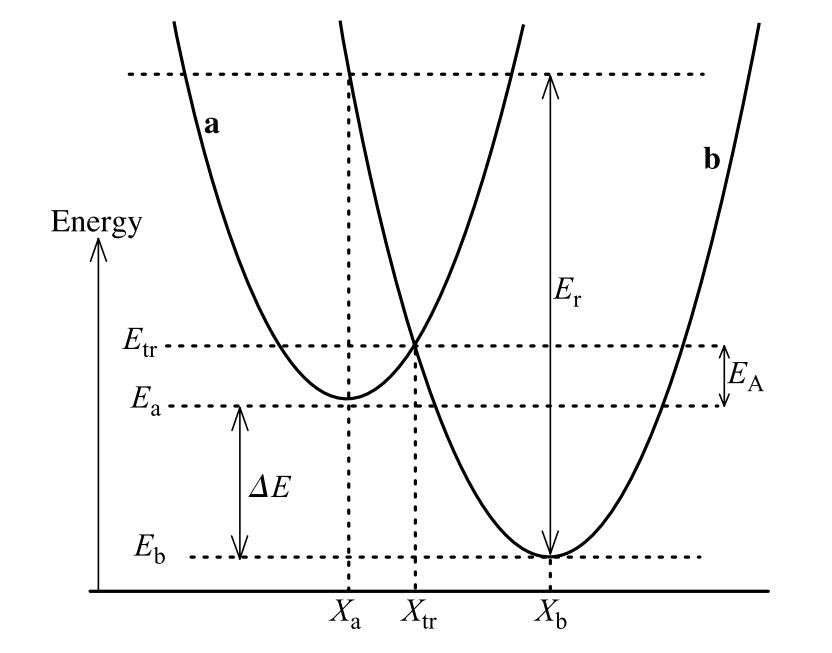
\includegraphics[width=10cm]{fig/Marcus.jpg}
          \caption{\textbf{Marcus理论的模型图}}
        \end{figure}

        在这样的近似下,我们就能画出一个类似于Figure \ref{Marcus figure}的模型图(原则上,图中的能量其实是自由能),根据平移谐振子近似,我们可以写出两个透热态势能面的能量
        \begin{equation*}
          Y_{a}=E_{a}+\frac{K}{2}\left(X-X_{a}\right)^{2}, Y_{b}=E_{b}+\frac{K}{2}\left(X-X_{b}\right)^{2}
        \end{equation*}
        在这里我们定义重整能(Reorganization Energy):电子从第一个势能面底垂直跃迁到第二个势能面上之后,从这个位置驰豫到第二个势能面的基态需要的能量,即图中的$E_r$\footnote{不同地方定义略有区别,但是为了推出这个公式,都是等价的}。那么重整能的大小也很容易计算\footnote{在很多文献中,人们分析的是双分子过程,所以给出的重整能是我们公式的两倍}
        \begin{equation*}
          E_{r}=Y_{2}\left(X_{a}\right)-Y_{2}\left(X_{b}\right)=E_{b}+\frac{K}{2}\left(X_{a}-X_{b}\right)^{2}-E_{b}=\frac{K}{2}\left(X_{a}-X_{b}\right)^{2}
        \end{equation*}
        可以看到,图中两个势能面有一个交叉,我们就认为这个交叉点就是从a态到b态过程的过渡态,那么过渡态对应的反应坐标为
        \begin{equation*}
          \begin{array}{c}
            {Y_{a}\left(X_{\mathrm{tr}}\right)=Y_{b}\left(X_{\mathrm{tr}}\right)} \\
            {E_{a}+\frac{K}{2}\left(X_{\mathrm{tr}}-X_{a}\right)^{2}=E_{b}+\frac{K}{2}\left(X_{\mathrm{tr}}-X_{b}\right)^{2}} \\
            {E_{a}+\frac{K}{2}\left(X_{tr}^{2}-2 X_{a} X_{tr}+X_{a}^{2}\right)=E_{b}+\frac{K}{2}\left(X_{tr}^{2}-2 X_{b} X_{tr}+X_{b}^{2}\right)} \\
            {X_{\mathrm{tr}}=\frac{E_{a}-E_{b}+\frac{K}{2}\left(X_{a}^{2}-X_{b}^{2}\right)}{K\left(X_{a}-X_{b}\right)}}
          \end{array}
        \end{equation*}
        过渡态对应的能量为
        \begin{equation*}
          \begin{array}{l}
            {E\left(X_{\mathrm{tr}}\right)=E_{a}+\frac{K}{2}\left(X_{\mathrm{tr}}-X_{a}\right)^{2}} \\
            {=E_{a}+\frac{K}{2} \frac{\left[E_{a}-E_{b}+\frac{K}{2}\left(X_{a}^{2}-X_{b}^{2}\right)-K X_{a}^{2}+K X_{a} X_{b}\right]^{2}}{K^{2}\left(X_{a}-X_{b}\right)^{2}}} \\
            {=E_{a}+\frac{K}{2} \frac{\left[E_{a}-E_{b}-K\left(X_{a}-X_{b}\right)^{2} / 2\right]^{2}}{K^{2}\left(X_{a}-X_{b}\right)^{2}}} \\
            {\therefore E_{A}=\frac{K}{2} \frac{\left[E_{a}-E_{b}-K\left(X_{a}-X_{b}\right)^{2} / 2\right]^{2}}{K^{2}\left(X_{a}-X_{b}\right)^{2}}=\frac{\left(\Delta E+E_{r}\right)^{2}}{4 E_{r}}}
          \end{array}
        \end{equation*}
        最后得到的$E_A=E\left(X_{\mathrm{tr}}\right)-E_a$是从a态到b态的活化能,$\Delta = E_b-E_a$是反应的反应能变,根据过渡态理论我们得到
        \begin{equation*}
          k_{r a t e}=A e^{-\frac{E_{A}}{k T}}=A e^{-\frac{\left(\Delta E+E_{r}\right)^{2}}{4 k T E_{r}}}
        \end{equation*}
        这就是Marcus理论的雏形,也是Marcus提出的函数形式,这个指前因子$A$,在透热极限下,是可以通过微扰法来计算推导的,最后的结果是
        \begin{equation}
          k=\frac{V^{2}}{\hbar} \sqrt{\frac{\pi}{\lambda k_{\mathrm{B}} T}} \exp \left(-\frac{\left(\lambda+\Delta G^{0}\right)^{2}}{4 \lambda k_{\mathrm{B}} T}\right)
          \label{Marcus theory}
        \end{equation}
        在式(\ref{Marcus theory})中,$V$代表了透热表象下两个态的相互作用(哈密顿量非对角元),我们按照通用的习惯,将重整能记为$\lambda$,反应的能量变化改为吉布斯自由能变。

        与经典过渡态理论告诉人们的一样,一个态到另一个态的转化,并不是能量下降越多速度越快的,Marcus理论的一个重要结论在于,当一开始$\Delta G^{0}$较大时,转化较慢,随着$\Delta G^{0}$减小,转化速度逐渐加快,这个速度的最大值,就是当$\Delta G^{0} = -\Lambda$时,在这之后,如果继续降低第二个态的能量,这个转化速度反而会下降。$\Delta G^{0}< -\lambda$的区域,通常称为Marcus反转区。

        但是过渡态理论和Marcus理论并非这么简单就结束了,它隐含着丰富的内涵。我们知道电子的运动速度是远快于原子核的,这也是BO近似的来源。在跃迁的理论中,我们会有被称为Franck-Condon原理的理论:电子的跃迁是垂直跃迁,即在势能面上,电子跃迁的瞬间原子核的位置(反应坐标)是不变的。那么问题来了,当体系处于光辐射下,电子跃迁的能量差是由外界辐射能量提供的,但是对没有外界辐射时,电子的能量是由热能,即原子核振动的能量提供的,因此实际上电子跃迁只发生在了两个态上相互作用最大,通常是能量最近的能级(电子能级加核振动能级)附近,所以电子态的跃迁问题其实是一个电子-声子(核振动)耦合的问题。Marcus理论对这个过程中的电-声子耦合的作用浓缩在了一个重整能里,这样的描述显然是充分的。

      \section{势间跳跃方法与FSSH}
        势间跳跃 (Surface Hopping)方法是一种混合量子经典(Mixed-Quantum-Classical)方法\footnote{需要注意混合量子经典与半经典方法(Semi-Classical)不同,前者一般指方法中既有经典部分又有量子部分,后者偏向量子力学做经典近似,演化一个半量子半经典的方程},它是非绝热动力学中非常常用的一类,尽管很早就有类似的思路,直到1990年John Tully提出了最少跃迁的势间跳跃(Fewest Switches Surface Hopping, FSSH)方法\cite{Tully1990},在这之后surface hopping方法被大量使用并且一直被发展,王老师课题组的核心研究方向就是SH方法中某些复杂问题的处理以及将其往更大体系更多自由度推广。

        在势间跳跃方法,原子核做经典处理,按照分子动力学的方法运动,但是其感受到的势能是由电子势能而非力场提供,电子的势能是根据电子的\sch 方程描述的,即电子的运动是量子处理。简单地说,如果读者熟悉分子动力学,那么这套方法理解起来是非常容易的,它的思路非常平凡,即在一个某一个时刻开始,在$\ud t$的时间间隔内用经典方法演化核的运动,然后计算电子波函数在这个$\ud t$内的演化,电子势能梯度为原子核的运动提供力,进而演化下一个时刻的原子核运动和电子运动,如此重复,就可以得到非绝热动力学的模拟结果。

        当然尽管图像上非常简单,但是实际操作起来会有各种各样的问题,比如下一小节中稍微涉及的势能面交叉和退相干的问题,包括电子如何在势能面上运动,都是现在仍然在讨论的重要问题,我们都会稍作涉及,但是首先要回到最早的FSSH方法上来。

        之所以称为Surface Hopping,就是因为在这套方法中电子的运动其实是在势能面间的跳跃,在特定的时刻内,电子只会存在于其中的某一个势能面(即通常说的active态),不同的SH方法的核心区别通常在于如何定义电子在不同势能面之间的跃迁概率,什么时候会跃迁。当然如果我们研究一个简单的隧穿问题,单一的SH计算只会得到一个固定的结果,要么穿过了势垒要么被反射等等,不会得到具体的隧穿概率数据,因此SH方法通常需要做很多次轨迹,然后取轨迹平均来得到物理观测量的结果。

        在等式(\ref{time-depend-coeff})中,我们演化波函数的系数,但是为了方便,我们会使用密度矩阵的演化,在等式(\ref{linear combination})的展开形式下,密度矩阵的矩阵元定义为$a_{kj}=c_k c_j^*$,在这个两边取时间导数并将(\ref{time-depend-coeff})的结果代入,我们就得到了关键性的等式
        \begin{equation}
          \begin{aligned}
            i \hbar \dot{a}_{k j}=& \sum_{l}\left\{a_{l j}\left[V_{k l}-i \hbar \dot{\vb*{R}} \cdot \vb*{d}_{k l}\right]\right.\\
            &\left. -a_{k l}\left[V_{l j}-i \hbar \dot{\vb*{R}} \cdot \vb*{d}_{i j}\right] \right\}
          \end{aligned}
          \label{time-de DM}
        \end{equation}
        我们通常关心的是密度矩阵的对角元,就是总电子波函数在某个势能面上的\textbf{布居}(\textbf{Population}),令上式中的$k=j$我们得到
        \begin{equation}
          \dot{a}_{k k}=\sum_{l \neq k} b_{k l}
        \end{equation}
        其中
        \begin{equation}
          b_{k l}=2 \hbar^{-1} \operatorname{Im}\left(a_{k l}^{*} V_{k l}\right)-2 \operatorname{Re}\left(a_{k l}^{*} \dot{\vb*{R}} \cdot \vb*{d}_{k l}\right)
          \label{time-de DM diagnol}
        \end{equation}
        而$\dot{a}_{k k}$就是势能面$k$上的布居变化,这里我们引入最少跳跃(Fewest Switches, FS)的思想,即在一个时间间隔$\ud t$内的布居变化完全由当前态向其他态的跃迁提供,以两个态的体系为例,如果在时间$t$时,假设所有轨迹中电子当前处在1态的轨迹数为$N_1(t)=a_{11}(t)N$,其中$a_{11}$是$t$时刻电子在1态的布居,$N$为总轨迹数。与之类似,我们有$t$时刻处于2态的轨迹数$N_2(t)=a_{22}(t)N$,在很小的时间间隔$\ud t$之后,两个布居为$a_{11}(t+\ud t)$和$a_{22}(t+\ud t)$,不失一般性,我们假设$a_{11}(t)<a_{11}(t+\ud t),a_{22}(t)>a_{22}(t+\ud t)$,我们就固定这个时间间隔内从态1跃迁到态2的轨迹数为$a_{11}(t+\ud t)-a_{11}(t)$,而从态2跃迁到态1的轨迹数为$0$,原则上可以两者各加一个常数,FS的思想等价于固定这个常数为$0$。这样处理之后,我们得到$\dot{a}_{22}=-\dot{a}_{11}=\frac{a_{11}(t)-a_{11}(t+\ud t)}{\ud t}$,则如下定义的跃迁概率
        \begin{equation}
          P_{1\rightarrow2}\equiv\frac{a_{11}(t)-a_{11}(t+\ud t)}{a_{11}(t)}=\frac{\dot{a}_{22} \ud t }{ a_{11}(t)}
        \end{equation}
        如果只有两个能级,将等式(\ref{time-de DM diagnol})代入得到
        \begin{equation}
          P_{1\rightarrow2}=\frac{b_{21} \ud t }{ a_{11}(t)}
          \label{hopping probability}
        \end{equation}
        上式就是FSSH的核心公式\footnote{细心的读者可能会发现与Tully原文中的分母不完全相同,但是本文的推导更加合理一点,通常也是使用这一套公式,当然,由于$\vb*{d}t$内密度矩阵几乎不会变化,究竟是用$t$时刻还是$t+\vb*{d}t$时刻对结果的影响不大。}。FSSH单个轨迹的流程就是先初始化,赋予研究的体系一个初始动能(动量)和位置,然后每个$\vb*{d}t$内先用经典力学的方法演化原子核的运动,再利用等式(\ref{hopping probability})计算出当前态跃迁到其他态的概率,用随机数的方法判断是否跃迁,同时还要判断跃迁之后是否满足能量守恒,如果满足,则完成跃迁并修正体系原子核运动的速度,不断重复上述过程就得到了动力学演化的结果。

        也许很多读者都会需要写FSSH的代码来学习部分工作,我们的细节部分就不再仔细展开,各位读者可以在实践中体会上面这段话的核心意义。我们需要提醒读者一个矛盾点,那就是虽然在势间跳跃方法中我们有电子的波函数和对应的密度矩阵,但是FSSH中的电子态并不是由这个波函数描述的。电子在哪个能级上并不是由展开系数决定的,而是有一个所谓active态的存在用来标记电子是在哪个能级上。这样其实说明FSSH中的电子波函数系数只是一个辅助工具,是一个辅助用来计算当前点的统计性质的工具,这个性质就是跃迁概率,然后通过不同轨迹做统计平均,才是FSSH的核心。
        
      \section{鸟瞰SH方法中的特殊问题}
        本小节将会简要地介绍在SH发展这么多年来,出现的很多问题,包括王老师组学长学姐在这方面的工作的简介,但是由于编者水平有限,只能略作介绍,并且有很大概率在细节上理解不全面甚至有错误,而王老师课题组的各位学长学姐在这方面有更多可说的内容。

        \paragraph{Trivial Crossing:}在势能面上演化动力学的过程中,势能面通常会有各类的交叉和相互作用,多数可以归为Trivial Crossing或者Avoided Crossing,两者的定义Figure \ref{two kinds of crossing}所示
        \begin{figure}
          \centering
          \label{two kinds of crossing}
          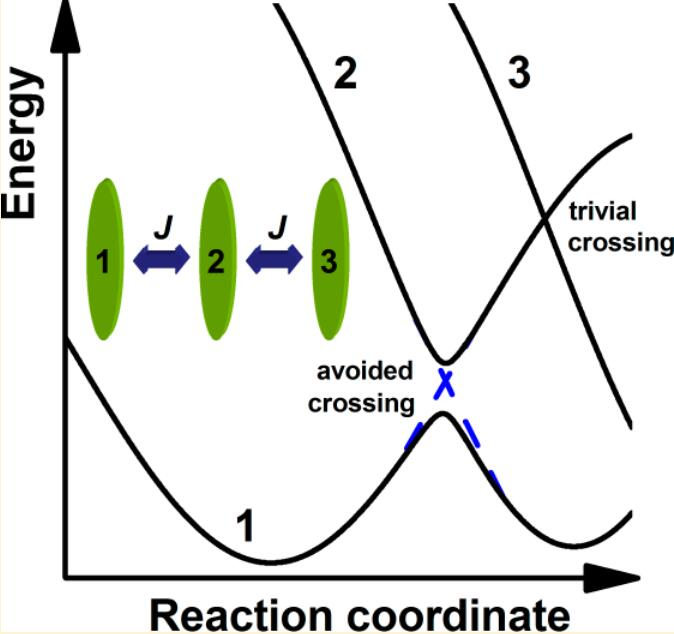
\includegraphics[width = 8cm]{fig/crossing.jpg}
          \caption{\textbf{SH两种Crossing的定义}}
        \end{figure}
        图中表示分子1和2之间有相互作用,当它们的势能面交叉时就会产生Avoided Crossing,1和3之间由于距离较远没有相互作用,但是在能量空间下,它们对应的态可能十分接近,这样使得它们的势能面存在交叉,即为Trivial Crossing。另外,Trival Crossing并非只存在于实空间距离很远的两个分子上,即使在同一个分子中,由于轨道之间没有或者相互作用非常小(比如对称性不同的分子轨道,$\sigma$键和$\pi$键之间)但是能量接近,也是可能发生Trivial Crossing的。

        但是由于电子结构计算是按照能量排序的,所以在发生Trivial Crossing的地方会有能级顺序的错误,误将别处毫不相关的能级作为了当前能级,而且根据等式(\ref{analytical dij}),此处的NAC是无法被描述的,通常会由于数值计算时过大而使得跃迁概率接近1,发生不该发生的跃迁,比如从分子1直接跳到分子3。

        为了处理这类问题,王老师发展了很多相关方法,这也是王老师前几年工作的重心。比如SC-FSS和CC-FSSH,后者把常见的Trivial Crossing进行了分类,每一类都有对应的解决方案,基本已经可以处理此类问题,具体内容可以参阅相关文章\cite{wang2014simple}\cite{Qiu2018}\cite{Bai2018}。

        \paragraph{超交换问题:}我们继续用上文中的图,同时联想化学里的过渡态理论,如果只有1态和2态之间、2态和3态之间有相互作用,但是1态和3态之间没有,按照SH方法的处理,如果想从1态到3态必须经过2态,但如果此时2态有较高的能量,高于此时原子核运动的动能,如果跃迁发生,就不满足能量守恒,尽管1态和3态之间的势能差可以被原子核动能满足,由于SH的操作方法,系统是不可能从1态到达3态的。但这并非真实情况,在量子力学中存在隧穿行为,因此实际上体系是会从1态到达3态的,SH这个错误的来源是忽略了原子核的量子效应导致的。当然,这不意味着SH不能处理超交换问题,王老师提出了在Liouville空间下Surface Hopping\cite{wang2015fewest},可以很好地处理超交换和隧穿的问题。

        \paragraph{退相干:}Surface Hopping方法中最大的短板之一就是被称为“过相干(over-coherence)”的现象。为了介绍这种现象,我们先回忆一下FSSH,我们利用运动方程来演化经典的原子核运动和量子的电子演化,这里其实存在一个问题,即使电子的状态和核受力是预先对应好的,但是两者运动的自洽性仍然难以保证。全量子的方法可以保证这个自洽性的存在,SH对原子核的经典处理是过相干现象的缘由。

        在一个单一的轨迹中,不同电子态的电子的运动是一直耦合在一起的,如果在某些情况下,原子核在两个势能面上的受力相差较大,甚至反向,在真实的全量子演化下,两个势能面上的原子核的波包将会分离,这也将导致电子波函数分离成两个部分,不再耦合在一起,然而原始的FSSH方法是无法处理这种退相干(decoherence\footnote{在王老师课题组的文章中有时称为Branching Correction, BC})现象的。因此正确的退相干策略也是SH方法发展的重要主题。
        
        \paragraph{相位修正:}传统的FSSH方法在处理不同势能面的波函数时会有一个相位差的问题。这个问题的来源是当FSSH决定电子要跃迁时,电子是直接跃迁到当前原子核结构下的其他势能面。但是由于势能面的能量不同,其对应的原子核速度不同,以两能级系统举例,如果两个原子核波包同时开始演化,电子一开始位于基态势能面,能量较高的势能面原子核速度较低(这是能量守恒的要求),因此在电子跃迁时,相同相位对应的激发态还未运动到基态波函数对应的位置,而是在其之前,这要求实际操作电子跃迁时,需要对波函数的相位进行修正(Phase Correction)。

    \chapter{全局优化问题}
      全局优化问题其实是个数学问题,简单地说就是有一个复杂的高维函数,我们如何求得其最小值的问题,但是这个数学问题在化学物理等领域都有重要的意义,我们也主要是全局优化算法在我们的问题中的应用。以最常见的也是王老师课题组之前处理的一个例子,如果任意两个原子之间的相互作用势能是LJ势,给定两个原子,可以通过对坐标求导等于0的方式找到这两个原子的最稳定的位置,但是如果是三个原子,事情就会变得麻烦起来,那如果是一千个原子呢?事实证明当原子数到13个时,极小值点就有至少1000个。这个问题其实等价于一个三千维的函数的最小值问题,想通过简单的解析方法求解是几乎不可能的。即使人们有强大的计算机,这样的一个问题还是不简单的,尤其是自由度增多时额外增加的计算量更是不可估计的。人们基于各种各样的思路发展了一系列全局优化算法,限于编者水平,在这里我们只能简单介绍其中的几种,主要参考了文献\cite{Kaplan2006}\cite{卡普兰2013分子间相互作用}。

      我们就以分子原子团簇的优化举例子,我们希望优化的函数是体系总能量。按照思路大致可以分为两类,迭代优化法和分而治之法(divide-and-conquer)。所谓迭代优化法就是从一个初始构型出发,进行迭代优化尽可能寻找极小值。我们先介绍一种最简单的思路,那就是梯度下降,即使是高维函数,你总是可以通过数值的方法求解这一点上能量关于某个自由度的导数(梯度),然后沿着负导数的方向移动,直到达到导数为0为止。这相当于沿着受力的方向一路运动直到达到一个极小值,这种方法的问题也是显然的,就是我们只能达到极小值而非最小值,当自由度非常多时,体系的极小值点可能非常之多,我们一般称这种方法为局部优化,譬如高斯等软件计算分子的最优构型时就是用的类似的思路(当然不是类似LJ势的分子力场的势能,而是量子化学计算的势能)。

      为了尽可能找到极小值,我们需要尽可能搜查整个势能面(直接遍历的计算量是巨大的,但是小体系少自由度情况也可以做),这意味着我们有时需要反着能量下降的方向运动进而跨过一些势垒区域,但是我们又不需要跨越太大的无意义的势垒,解决这个问题就是利用Monte Carlo模拟中接受分子构型的类似方法,认为有一个所谓的温度存在,即不是能量最低原理,而是满足某种分布。在全局优化问题里,我们不一定采用玻尔兹曼分布型的函数,原则上为了达成目的的任何函数形式都可以。当体系沿着某一个自由度能量升高时,用这个函数来判断是否接受构型。

      分而治之的思路就是将体系分为多个问题,每次优化其中的一部分,然后将这些分别处理的部分按照某种办法拼接起来,就可以得到全局问题的解,为了保证最终的结果的可靠性,划分子问题和对所有子问题的拼接构成了分而治之方法最大的关键点和难度。这两个思路是全局优化方法的基础,我们通常是多种思路混合得到最后的算法。正如刚刚说的,全局优化算法里可以用遍历的方法寻找最小值,这是最简单粗暴计算量最大的,另一个极端就是完全取随机构型,然后比较取到的随机构型的能量然后从中选中最小的。显然这两种方法都不是特别靠谱,接下来我们介绍一种现在常用几种全局优化算法。
      
      \section{模拟退火算法}
        全局优化算法中有一类比较出名的叫做模拟退火算法(Simulated Annealing, SA)。最早由Kirkpatrick提出,其原理是类比从实验中的熔融固体生长单晶的过程:首先,固体在高温下熔化,然后温度缓慢下降,在凝固点附近停留相当长的时间,这会使得亚稳态的晶型逐渐转化为最稳定的晶型,等价于在势能面上最小值的生成。
        
        对于分子的能量优化这个问题,在这个系统中有一个温度的概念,使得体系某种程度上形成一个正则系综。根据能量均分原理,这个温度某种程度上相对应着体系的总能量,每一个自由度有$kT/2$的能量。这个算法的核心思路是先升温,使得体系处于一个较高的温度下,也就是拥有一个较高的能量,使得体系“熔化”,这样它在随机变化过程中就可以克服很高的势垒,进而有可能遍历势能面上尽可能多的位置,然后降温(退火),原本在势能面不同位置的分子能量逐渐减小,在每个温度时逗留的时间足够长,这样他们的运动按照玻尔兹曼分布,进而在每个温度上尽可能地跨越当前的势垒,来保证它们不会困在某个亚稳态。退火算法的优势明显,它只是在原本的玻尔兹曼分布的全局优化基础上添加了对体系能量的控制,非常容易结合到代码之中,缺点也非常明显。体系在这样退火的过程中很容易掉进一个“很深”的局部极小值点而非体系的最小值。

        在这个基础上,为了使得体系能穿过极小值附近的势垒,人们引入了量子力学中的隧穿、离域的概念,进而发展了各类量子退火算法(Quantum Annealing, QA)。将体系视为一个“波包”,随着时间的演化,波包可以穿透势垒,本章参考文献中还简要提及了基于QA的高斯密度退火算法和量子路径极小化方法,感兴趣的读者可以阅读相关内容。
      \section{超曲面形变方法}
        这类全局优化方法是通过对势能面的函数进行某种变换来实现的,一般的变换策略由Stillinger和Weber提出,他们希望通过变化的势能面能够拥有两个性质:较浅的局域极小值在变换后数目将大大减少甚至消失;全局极小值在势能面的变形中是连续变化的,并且整个过程中,最小值点只有一个,并且对应体系的最小值点。

        这类方法常见的有两类,扩散方程法(Diffusion Equation Method, DEM)和阱间跳跃方法(Basin Hopping Method)。扩散方程法的思路比较数学,就是用一个数学变换,比如说
        \begin{equation*}
          f^{[1]}(x) = f(x) + \beta f^{\prime \prime}(x), \beta>0
        \end{equation*}
        读者可以验证,这种方法可以让一个大于二次的多项式的一维的势能函数的势阱变浅,势垒变矮。对于新得到的函数不断进行这个变换,取$\beta = t/N$,我们得到
        \begin{equation*}
          f^{[N]}(x) = \left(1+\frac{t}{N}\frac{\ud^2}{\ud x^2}\right)^N f(x)\rightarrow \exp\left(t\frac{\ud^2}{\ud x^2}\right)f(x)
        \end{equation*}
        如果将$N$趋向于无穷的函数称为$F(x,t)$,可以看出,这个方程满足
        \begin{equation*}
          \frac{\partial F}{\partial t} = \frac{\partial^2 F}{\partial x^2}
        \end{equation*}
        即经典的扩散方程的形式,它的初值条件为$F(x,0)=f(x)$,这也是扩散方程法名字的由来。利用优化后的函数$F$就可以更容易地完成全局优化问题,DEM算法在很多体系都有不错的应用价值。

        第二类方法就是阱间跳跃算法,BH算法严格来说定义了一个从连续的位形空间向一组局域的极小值点的映射。它的思想是把所有的势垒都拉低到极小值的位置,将整个复杂的势能面变化成一些平坦的basin,效果就如Figure \ref{BH}所示。
        \begin{figure}
          \centering
          \label{BH}
          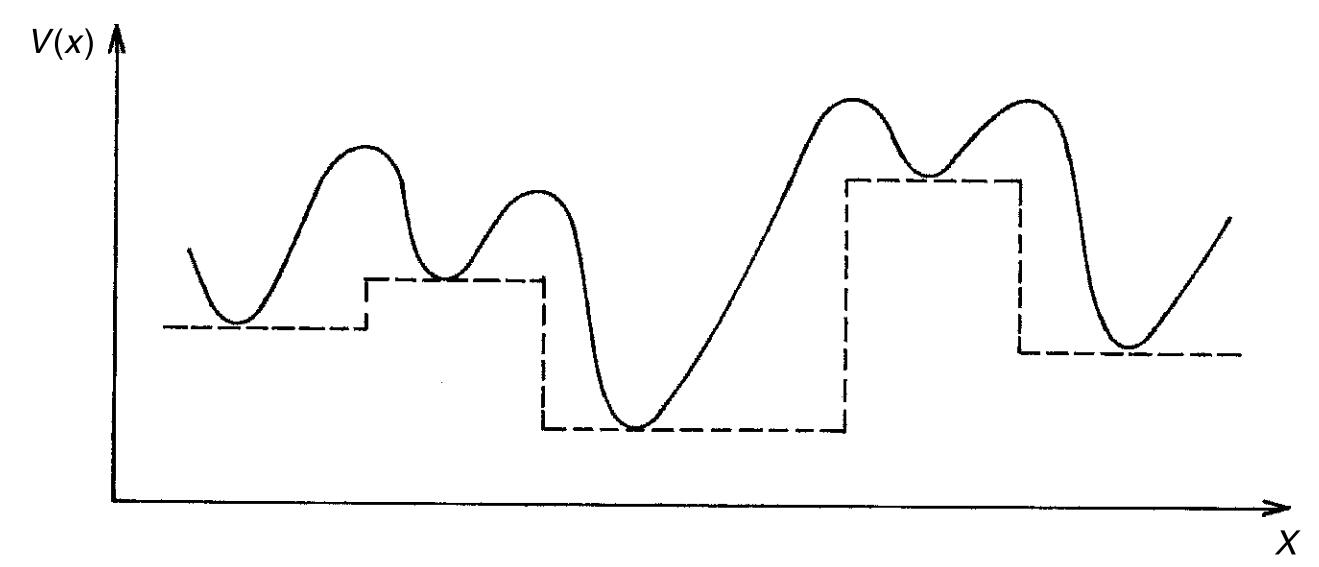
\includegraphics[width = 12cm]{fig/BH.jpg}
          \caption{\textbf{Basin Hopping方法对势能面的处理}}
        \end{figure}
        阱间跳跃方法通常会与恒定“温度”下的Monte Carlo方法结合,相对简单粗暴,也是王老师组处理LJ团簇的方法。简单的说,核心思路为我先有一初始的分子构型,然后对其进行局部优化得到一个局部优化的结构和对应的能量。然后在这个构型上每个自由度随机移动一点从这个随机移动得到的构型再做局部优化,如此反复,直到有足够多的极小值,来构成basin势能面,然后在这个势能面上用经典MC的方法优化,试图从中挑出最小的那个。这个方法十分简单有效:跨过一些势垒尽可能遍历相空间。而王老师课题组还在这里面加入了多很多为了节省计算量的功能,具体细节只有仔细看过代码才能理解。但是其中非常关键的一部分就是把绝大多数的优化在离空间内完成,这样原子间的能量就不用每次都计算,而是把离散空间每个格点距离的能量提前算好保存在一个数组里,以后每使用时只需要调用数组元素就行了。

      \section{遗传算法}
        另一类比较火爆的思路就是遗传算法(Genetic Algorithm, GA),这是一个借鉴生物遗传进化的非常有趣的算法,全局优化问题可能的解被视为参与遗传竞争的个体。
        
        在该算法的典型应用中,空间中的某个点可以用一个固定长度的二进制数组表示,这是与生物中的染色体进行类比。开始时,就选用任意一定个数的点作为初始“种群”,每一个点都是一个个体,通过计算这样的团簇结构的能量来评估这个种群中每一个个体的适应程度(fitness)。将初始种群中的每个个体按照适应程度进行排序,可以选出其中适应程度较高的点“繁殖”出下一代的种群。
        
        “繁殖”的过程往往是遗传算法的核心,通常包括如实复制、交叉互换和突变三部分构成。一种常见并且合理的做法是,对于具有较高适应程度的个体的二进制序列进行如实复制,直接得到下一代的个体,这个个体与亲代中的个体完全一致,这种复制过程可以保证体系搜索的点集中在具有较高的适应度的点附近。交叉互换是将一部分或者是全部的序列进行两两配对,类比生物的DNA复制的交叉互换过程,将其中的一段序列切开并且进行交换,交叉互换是GA中的基本操作。而突变,顾名思义,就是将某个任意位置上的序列发生一个随机的变化,突变的概率通常控制较低,以保证“进化”的过程中较好的“基因”不会失去。突变的随机性,保证了体系种群在进化过程中不至于完全单一,这就保证了体系很难一直处于某个难以跳出的极小值位置。

        所得到的第二代序列继续按照相同的做法计算适应度,然后繁殖出第三代,如此反复,直到整个种群个体的适应度不再有提升,为了搜索势能面的更多区域,GA还可以采用多个种群同时演化的策略,甚至在演化过程中种群之间的也有“基因”的交流,这样可以保证遗传算法在寻找全局最小值的效率。当然可以看出,GA也有一个显著的缺点,即实现起来较为复杂。本章的参考文献中给出了一个详细的遗传算法的例子,有兴趣的同学可以自行查看。

        向生物学习是全局优化中的常见思路,除了遗传算法之外,现在还有基于蚂蚁寻找食物思路的算法等,不予详细介绍。另外,可以看出,机器学习在这方面也肯定有一定的建树,但是势能面通常过于复杂,简单的机器学习网络可能无法实现。

        最后需要提醒读者,全局优化的问题远远不限于分子能量优化上,包括求条件极值,减小误差,拟合等多种问题都可以使用全局优化的思路进行处理,有时候往往能产生有趣的效果。\sout{初一看只有一两个做全局优化的学长学姐,做到最后就会发现,组内一大半的人都在做全局优化}


    \chapter{离散变量表象(DVR)}
     
      DVR,即Discrete Variable Representation(离散变量表象),是量子力学目前为止最为可靠的数值计算体系特征值/特征向量/动力学演化的方法之一。鉴于在王老师课题组可能会经常听到DVR三个字母,并且很多时候都会作为动力学的精确解的参考,我们在这里单独为其整理出了一章。它的实现依赖于一个比较特殊的基组,使各类算符以矩阵的形式参与运算,利用成熟的线性代数方法求解。由于DVR的基础并不难,但是却有很多种表述的方法,文献中也时常只放公式而不谈理解,因此这里我们做一些必要的解释,由于不可描述的原因,我们给出了两种理解思路,第一种是先从基组定义sinc函数出发,自下而上地构建DVR的框架,另一种是放弃基组推导,从表象变换出发自上而下地构建DVR。 
      \section{从sinc函数基组出发的DVR}
        我们再来回顾一下完备基展开。我们对于一个可观测量的期望值$\langle \psi | \hat{A} | \psi \rangle $ ,我们期望引入一个正交完备归一的基组来进行展开,由于完备基性质,我们有
        \begin{equation}
      	  \langle \psi | \hat{A} | \psi \rangle = \sum_i \sum_j \langle \psi | e_i \rangle \langle e_i | \hat{A} | e_j \rangle \langle e_j | \psi \rangle 
        \end{equation}
        其中$| e_i \rangle $ 为一个完备基。如果稍微想一想,我们就能够发现它实质上等价于
        \begin{equation}
      	  \sum_i \sum_j \langle \psi | e_i \rangle \langle e_i | \hat{A} | e_j \rangle \langle e_j | \psi \rangle \equiv \Psi ^\dagger\mathbf{A} \Psi
        \end{equation}
        其中$\mathbf{A}, \Psi$分别为矩阵和向量,每个元素为
        \[
      	  \Psi_i = \langle e_i | \psi \rangle , A_{ij} = \langle e_i | \hat{A} | e_j \rangle 
        .\] 
        我们只要选取一个恰当的基组,我们就能够将复杂的偏微分方程问题转化为一个在计算机上更容易实现的线性代数问题。但基组选的不好内积的计算会非常复杂,反而不利于计算机实现。DVR便解决了这样的一个痛点,它的核心内容是
        \begin{center}
        	\textbf{将连续函数格点化(离散化)的同时提供可观测量的期望值。}
        \end{center}
        所谓离散变量表象,即将原本的波函数在一个对应着离散空间的表象上进行展开,我们举DVR中最为常用的基组为例,首先引入sinc 函数,定义为
        \begin{equation}
        	\mathrm{sinc} \, (x) \equiv \frac{\sin{\pi x}}{\pi x}  
        \end{equation}
        对实空间作离散化处理,如果我们关心的体系在某个范围内,我们将其分割成一个一个小格点,格点间距离定义为$\Delta x$,再有$x_i \equiv i\Delta x$,DVR中所选用基组为
        \begin{equation}
      	  \chi_j (x) \equiv \langle x | e_j \rangle = (\Delta x)^{-\frac{1}{2}}\, \sinc{\frac{x - j \Delta x}{\Delta x}} 
        \end{equation}
        明眼人一眼就能看出来,它有着神奇的性质
        \begin{equation}
        	\chi_i (x_j) = \sqrt{\frac{1}{\Delta x}} \delta_{ij}
        \end{equation}
        这正利用了正弦函数在 $n\pi$的节点上为零,而在 $x=0$处 $\sinc{x}$极限为 $1$.

        这能够让波函数离散化非常有用——我们通过选出足够多,足够密的格点,取每个点对应的函数值来代表原来的波函数,从而做到``离散的效果'',
        \begin{equation}
      	  \psi(x) \sim \sum_i c_i \chi_i (x_i) = \sum_i \sqrt{\Delta x} f(x_i) \chi_i (x) 
        \end{equation}
        或
        \begin{equation}
      	  \langle e_i | \psi \rangle = \sqrt{\Delta x} \,\psi(x_i) 
        \end{equation}
        这样我们就完成了第一步:波函数的离散化。

        我们再来看看这个基组是否满足正交归一。但这是一个$\mathrm{sinc}$函数,比较棘手,我们使用傅立叶变换来完成积分工作。

        首先我们来看看$\sinc{x}$的傅立叶变换。
        \[
        	\mathcal{F}[\sinc{x}] =  \frac{1}{2\pi}\int \sinc{x} e^{-ikx} \, \mathrm{d}x  = \frac{1}{2\pi}  \int \frac{\sin{\pi x}}{\pi x} e^{-ikx} \, \mathrm{d}x 
        .\]
        面对这个奇怪的积分的常见方法是让$\sin{x}$转换成 $e^{ix}$.当然这个会牵涉到实部和虚部的问题,我们便尝试通过 $\frac{e^{ix}-e^{-ix}}{2i}$来得到最终结果。不过我们还是先尝试康康$e^{ix}$的情况如何,
        \[
      	  \int \frac{e^{i\pi x}}{\pi x}e^{-ikx} \, \mathrm{d}x = \int \frac{e^{i(\pi -k) x}}{\pi x} \, \mathrm{d} x
        .\]
        于是我们便化简成为如何计算
        \[
      	  \int \frac{e^{ikx}}{x} \, \mathrm{d}x 
        .\] 
        这是一个在实轴上积分的经典老题。由于$x=0$ 处该函数存在一阶奇点\footnote{就是在该点对应阶数为$x^{-1}$的项使其发散。},我们需要让回路绕过这个点,使整一个复变函数处处可积。若$k>0$,我们取复平面中的下半平面作为回路,挖取那个奇点后平面就没有别的奇点了,因此回路积分为零,而无穷远处由于$e^{ikx}$的``压制''效果为零。因此我们只需考虑挖去那个奇点对应的积分,从而有
        \begin{equation}
      	  \int \frac{e^{ikx}}{x} \, \mathrm{d}x =  \pi i \, \mathrm{Res}\{\frac{e^{ikx}}{x}\} = \pi i \quad (k>0)
        \end{equation}
        $k<0$呢?我们做一个小小的变量代换,
        \[
          \int_{-\infty}^{+\infty} \frac{e^{ikx}}{x} \, \mathrm{d}x = \int_{-\infty}^{+\infty} \frac{e^{ikx}}{-x} \, \mathrm{d}(-x) =- \int \frac{e^{i|k|y}}{y} \, \mathrm{d} y   
        .\] 
        我们看到了在这个情况下的积分为原来的相反数。这两者结合起来我们就可以把它打包成为sign 函数,即
        \begin{equation}
      	  \int _{-\infty} ^{+\infty} \frac{e^{ikx}}{x} \, \mathrm{d}x = \pi i \, \mathrm{sign}\,(k) = 
      	  \begin{cases}
      	    \pi i, \, k>0 \\
      		  0, \, k=0 \\
      		  -\pi i, \, k<0
      	  \end{cases}
        \end{equation}
        让$k=0$时 $\mathrm{sign}\,(k)=0$是出于$\frac{1}{x}$ 为奇函数,在实轴上积分结果应为零的考虑。

        利用这个结果,我们就能反过来得出
        \begin{equation}
      	  \int \frac{e^{i(\pi-k)x}}{\pi x} \, \mathrm{d}x =  i \, \mathrm{sign}\, (\pi-k) 
        \end{equation}
        那么自然就有
        \begin{equation}
      	  \int \frac{e^{i(-\pi-k)x}}{\pi x} \, \mathrm{d}x = - i \,\mathrm{sign}\, (\pi + k) 
        \end{equation}
        再把这两个结果结合起来,我们就最终得到了
        \begin{equation}
      	  \mathcal{F}[\sinc{x}] = \frac{\mathrm{sign}\,(\pi-k)+ \mathrm{sign}\,(\pi+k)}{4 \pi}= \frac{1}{2 \pi}\mathrm{rect}\, (\frac{k}{2\pi}) =
      	  \begin{cases}
      		   \frac{1}{2\pi}, \, -\pi < k < \pi \\
      		  0, \, \text{otherwise}
      	  \end{cases}
        \end{equation}
        也就是$\sinc{x}$进行傅立叶变换后得到了矩形波!

        我们趁热打铁,继续看原来的基组的内积。

        还记得傅立叶变换的几条定理吗?有一条是把频谱中函数相乘转化为卷积,也就是
        \begin{equation}
      	  \mathcal{F}[f_1(x) * f_2(x)] = 2\pi F_1(k) F_2(k) 
        \end{equation}
        其实对于逆傅立叶变换也成立,也就是
        \begin{equation}
      	  \mathcal{F}[f_1(x) f_2(x)] = \frac{1}{2\pi} F_1(k) * F_2(k) 
        \end{equation}
        那么我们从原来的内积定义出发,
        \begin{align*}
        	\langle e_i | e_j \rangle &= \int _{-\infty}^\infty \frac{1}{\Delta x} \sinc{\frac{x- i \Delta x}{\Delta x}} \sinc{\frac{x- j \Delta x}{\Delta x}} \, \mathrm{d}x\\ 
      				   &= \frac{2\pi}{\Delta x} \mathcal{F}[\sinc{\frac{x - i\Delta x}{\Delta x}} \sinc{\frac{x- j \Delta x}{\Delta x}}] \bigg|_{k=0} \\
      				   &= \frac{\Delta x}{2\pi} \int e^{- I \xi (i-j) \Delta x} e^{-I k j \Delta x}\mathrm{rect}\, \left( \frac{\xi \Delta x}{2 \pi} \right)  \, \mathrm{rect} \, \left( \frac{(k-\xi) \Delta x}{2 \pi} \right) \, \mathrm{d} \xi \bigg|_{k=0} \\
      				   &= \frac{\Delta x}{2 \pi} \int _{-\frac{\Delta x}{\pi}} ^{\frac{\Delta x}{\pi}} e^{-I \xi (i-j) \Delta x}  \, \mathrm{d} \xi \\
      				   &= \sinc{i-j} 
        \end{align*}
        从而得到
        \begin{equation}
        	\langle e_i | e_j \rangle = \delta_{ij}
        \end{equation}
        上面的推导中充分利用了变量代换、延迟定理、\sout{\emph{Mathematica}}等技巧。$I$是为了与 $i$作区分,表示虚数单位。以这个为基础,我们还可以得到
        \begin{equation*}
      	  \langle e_i | - I \hbar \frac{d}{dx} | e_j \rangle = -i\hbar \left[ e^{-I k i \Delta x} \,\mathrm{rect}\, \left( \frac{k \Delta x}{2 \pi} \right)  \right] * \left( I k e^{- I k i \Delta x} \, \mathrm{rect} \, \left( \frac{k \Delta x }{ 2 \pi} \right)  \right) 
        \end{equation*}
        从而
        \begin{equation}
      	  \langle e_i | - I \hbar \frac{d}{dx} | e_j \rangle = -\frac{I \hbar (\sin (\pi  (i-j))+\pi  (j-i) \cos (\pi  (i-j)))}{\pi \Delta
          x (i-j)^2} = 
          \begin{cases}
         	  0, \, i=j \\
      	    \frac{I\hbar (-1)^{i-j}}{(i-j) \Delta x}
          \end{cases}
        \end{equation}
        进一步地,
        \begin{equation}
       	  \langle e_i | -\frac{\hbar ^2}{2m} \frac{d^2}{dx ^2} | e_j \rangle = \frac{\hbar^{2}(-1)^{i-j}}{2 m \Delta x^{2}} \begin{cases}{\pi^{2} / 3,} \quad {i=j} \\ {\frac{2}{\left(i-j\right)^{2}},} \quad {i \neq j}\end{cases}
        \end{equation}
        这样我们就凑出了动能对应的矩阵。

        位移期望值其实不需要上面这么麻烦,我们可以做一个简单的变换,
        \[
      	  \int \sinc{\frac{x- i \Delta x}{\Delta x}} x \sinc{\frac{x- j \Delta x}{\Delta x}}\, \mathrm{d} x = \int \sinc{\frac{x- i \Delta x}{x}} (x- \frac{i+j}{2}\Delta x) \sinc{\frac{x-j \Delta x}{x}}\, \mathrm{d}x
        .\] 
        利用对称性可以非常方便地得到
        \[
      	  \langle e_i | x | e_j \rangle = \delta_{ij} j \Delta x
        .\] 
       
        势能和波函数相似,也采用离散化的方式,从而有
        \begin{equation}
      	  V_ij = \langle e_i | V | e_j \rangle  = \delta_{ij} V(x_i)
        \end{equation}
        将这两个矩阵相加,我们就得到了在该基组下的\sout{哈密瓜}哈密顿矩阵。
        
      \section{从表象角度的DVR}
        任何一个\sch 方程的求解都必须依赖于一个表象,因此原则上我们可以选择坐标表象,只是坐标表象是连续的,而我们只能处理离散的问题,这就是DVR的出发点\footnote{这一部分极大地参考了求化2014沈一帆的笔记以及DVR的主要参考文献\cite{colbert1992novel}}。即我们需要找到一个well-defined离散表象,并且把已有的表象(一般是能量表象)做表象变换到这个离散表象下,也正因为我们无法使用完备的坐标表象,DVR有很多的小问题,按照组里师兄们的推导经验,DVR的坐标动量的对易关系就有一定问题。

        DVR的做法是只处理一个范围$[a,b]$内的波函数\footnote{这是一种箱归一化的方法,如果希望全空间,就是在这个基础上取$a$和$b$的极限}。因为可用的能量表象波函数就取为无限深势阱的解,我们有
        \begin{equation}
          \hat{H} | n \rangle = E_n | n \rangle,\;\; \Psi_n(x) = \sqrt{\frac{2}{b-a}}\sin\left(n\pi\frac{x-a}{b-a}\right)
        \end{equation}
        我们希望把它变换到一个离散的坐标表象下,我们先定义这个离散的坐标表象,使用一个等距离的格点选取方法,在$[a,b]$之间取$N+1$个格点:$\{x_0 = a,\dots x_i = a + \frac{i(b-a)}{N},\dots, x_N = b\}$,格点之间的距离为$\Delta x = \frac{b-a}{N}$。
        
        而真正的坐标表象的基函数是$\delta$函数\footnote{这个写法的意思是坐标表象的基函数$ |x_i\rangle $写成$x$的函数的表达式,若读者十分迷惑,可以参考量子力学态矢量那一节}$ \langle x | x_i \rangle =\delta(x-x_i)$,从这个角度出发,它们显然是正交归一到$\delta$函数的,但这个不是我们想要的,因为它无法在离散的意义下归一化,因为我们计算它们的内积的时候插入能量表象的完备基
        \begin{equation}
          \begin{aligned}
            \langle x_i | x_j \rangle &= \sum_n^{\infty} \langle x_i | n \rangle \langle n | x_j \rangle = \frac{2}{b-a}\sum_n^{\infty}\sin\left(n\pi\frac{x_i-a}{b-a}\right)\sin\left(n\pi\frac{x_j-a}{b-a}\right)\\
            &=\lim_{N\to \infty}\frac{2}{N\Delta x}\sum_{n}^{N-1}\sin\frac{n\pi i}{N}\sin\frac{n\pi j}{N}
          \end{aligned}
        \end{equation}
        上式可以最后推出一个解析的表达式,这个过程相对繁琐,基本思路就是套用三角恒等式,以及把$\sin$函数换成复数,求和就会变为等比数列求和,最后求$N\to \infty$的极限,上式最终结果为
        \begin{equation}
          \frac{1}{\Delta x}\left[\frac{\sin (i-j)\pi}{(i-j)\pi}-\frac{\sin(i+j)\pi}{(i+j)\pi}\right]
        \end{equation}
        可以看到如果$i\neq j$,由于他们都是整数,所以上式为$0$,$i\to j$的极限下,第二项为$0$,最终结果为$\frac{1}{\Delta x}$。当然因为我们取了有限范围$[a,b]$又取$N\to \infty$所以这个等价于$\delta$函数,但这就让我们有一种让离散基组归一化的方法,即基组为$ | x_i^{\prime} \rangle = \sqrt{\Delta x} | x_i \rangle$。我们先不管这个基组表达式具体为何,我们已经定义了一套正交归一的不完备基,只有$x_i$遍历全部实数才是完备的。此后为了方便我们省去一撇。

        然后在这个基组下可以求出力学量的矩阵形式。
        \begin{equation}
          A_{ij}=\langle x_i | \hat{A} | x_j \rangle = \sum_{mn} \langle x_i | m \rangle \langle m | \hat{A} | n \rangle \langle n | x_j \rangle 
        \end{equation}
        由于$ | m \rangle $是无限深势阱哈密顿量的本征态,对于任何一个和哈密顿量共享本征态的力学量(也就是与哈密顿量对易的力学量)\footnote{值得一提的是,在对$[a,b]$推广到负无穷和正无穷的极限下,$\Psi_n$就会变为平面波,这样一来,便对动量算符也成立},上式的$ \langle m | \hat{A} | n \rangle $就只有对角元,上式进一步化简为
        \begin{equation}
          A_{ij} = \sum_{n} \langle x_i | n \rangle A_n \langle n | x_j \rangle \\=\Delta x \sum_{n} \Psi_n(x_i) A_n \Psi_n(x_j)
        \end{equation}
        其中$\Psi$就是本节第一个公式中的无限深势阱本征态。

        举几个简单的例子,对于势能,对$x$积分中,可以想象成一个常数,所以可以直接从中心提出来,最后结果为$V(x_i)\delta_{ij}$\footnote{当然这对所有只含坐标的力学量都成立}。对于动能,则相对麻烦一些
        \begin{equation}
          T_{ij}=\frac{\hbar^2}{2m}\left(\frac{\pi}{b-a}\right)^2\frac{2}{N}\sum_n^{N-1}n^2\sin\left(\frac{n\pi i}{N}\right)\sin\left(\frac{n\pi j}{N}\right)
        \end{equation}
        上式仍然可以解析得到,得到结果之后把$[a,b]$向不同的范围推广,就可以得到多种坐标系下的计算结果。我们就不再继续往下推了,这些结论都可以参考最经典的那份文献\cite{colbert1992novel}的附录A。
      \section{DVR的应用}
        其实根据Miller文章的公式,我们就已经能很简单地实现一个一维DVR程序了,但是也许读者还没有建立这两者之间的直接链接,因此我们最后做一小节的总结。

        首先,我们需要强调的是,根据上面的叙述,DVR相当于选择了一个基组,并且是有限的离散的基组,并且我们已经知道了动能算符和势能算符在上述基组下的矩阵形式的表达式,即使你完全没有看懂这些公式的推导,按照他们的结论你仍然可以把这个有限坐标表象的哈密顿量写出来。那只要有了哈密顿量,自然就可以想做什么做什么。
        
        那么不懂事的读者就会问了,有了哈密顿量之后我们能干啥呢?第一就是直接解定态\sch 方程啦。所以只要我们把哈密顿量在上述基组里写出来,做对角化,就能得到能量了。对于一维问题来说,这个过程非常简单,如果读者不只希望看个热闹,我们建议读者可以写一个一维谐振子的DVR程序,我保证500行和一下午时间之内就可以搞定。可以大大加深对DVR的理解。

        当然有了$\hat{H}$之后,我们能解的不只是定态\sch 方程,我们当然可以用哈密顿量和含时\sch 方程做动力学演化,但对于这个,我们还需要一些\sout{微操}技巧。我们将薛定谔方程关于时间也离散化,
        \[
      	  \hat{H}(t) \psi(x;t) = i \hbar \frac{\partial }{\partial t} \psi(x;t) \Rightarrow \left[\mathbf{E} \hbar + \frac{i \Delta t}{2} \mathbf{H}(t+\frac{\Delta t}{2})\right] \psi(t+ \Delta t) = \left[\mathbf{E} \hbar - \frac{i \Delta t}{2} \mathbf{H} (t+\frac{\Delta t}{2})\right] \psi(t)  
        .\] 
        这可以从$\frac{\partial }{\partial t} \psi(t) \sim \frac{\psi(t+ \Delta t) - \psi(t-\Delta t)}{2 \Delta t}$ 得到\footnote{而如果用欧拉法近似,会使波函数摸值发散。若有兴趣可自行证明。},以及$\mathbf{E}$表示单位矩阵。

        \begin{figure}[h]
          \centering
          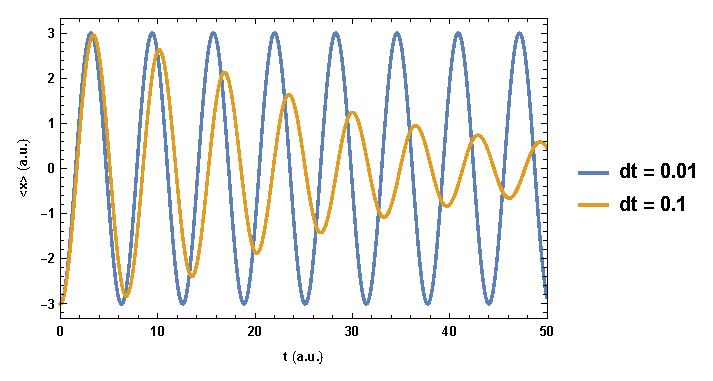
\includegraphics[width=0.8\textwidth]{fig/DVRtest.eps}
          \caption{谐振势下的一个典型的DVR结果}
          \label{DVRresult}
        \end{figure}

        将以上动态演化的方法综合起来便能得到一个完整的一维DVR动力学模拟程序,比如\url{https://github.com/Walter-Feng/SincDVR}。一个典型模型,谐振势下一个高斯波包的演化的DVR结果如 Figure \ref{DVRresult} 所示。可以看出在一个足够小的时间间隔 dt 下体系能够很好地呈现震荡,而如果\sout{一不小心}选取较大 dt 便会呈现一个阻尼震荡的错误结果。因此虽然DVR能够成为量子力学精确解的``范本'',足够细致的取点和时间演化是结果具有信任度的关键,这也导致了DVR的耗时往往很长。这也部分说明了王老师的课题组大力发展非绝热动力学方法的动力所在——我们确实可以有精确解,但它实在是太慢了。

        DVR其实并不仅限于一维。我们从前面的章节中已能隐约感受到,只要我对每个维度进行这样的基组展开,我们就能够对多维度体系进行能量求解和动力学模拟。多维的势能仍然只有对角元,动能可以参考文献\cite{colbert1992novel}的公式(2.6)。

        最后给出一点评论,DVR原则上可以解任何问题,但它是一个实空间的全量子方法,所以它的自由度是$3N$级别的,也就是计算量是关于我们关心的粒子数目指数增长的。至今为止也最多处理十几个自由度,因此处理分子中的电子结构问题是几乎不可能的。在量子化学中,DVR主要用来处理几个原子以下的分子的原子核的全量子解,比如精确的振动能级和原子核演化的动力学等。而后者也正是surface hopping处理的问题,所以DVR在王老师课题组通常可以作为标准结果用来对比。

    \chapter{相空间-量子哈密顿动力学(PS-QHD)}
      \label{phase_space_dynamics}
      \begin{enumerate}
        \item 在更多的化学问题中,电子会发生跃迁,Born-Oppenheimer近似失效,比如光催化反应,光电材料中的电荷传输,无辐射跃迁,生命活动中的光合作用,呼吸作用等,必须使用更普适的非绝热动力学研究。

        \item 非绝热动力学的思想分为两派:追求严格,将电子与原子核做量子化处理;追求效率,将原子核作经典处理。需要在拥有量子效应的基础上保证计算效率。David Manolopoulos 提出的环聚合物方法(ring polimer)是一种可能,并已被John Tully和Frank Huo等人与面间跳跃方法相结合。而该方法只能处理热力学平衡态,但很多化学过程发生在非平衡态。Oleg Prezhdo提出的量子哈密顿动力学(QHD)是另一种可能。

        \item QHD从经典描述出发,逐级添加量子效应修正,添加无穷阶修正即可达到全量子严格解。

        \item QHD用Hilbert空间描述,以一系列算符的期望值作为变量组来描述粒子的运动过程。由于经典力学中确定粒子的运动状态只需要坐标和动量,因此HS-QHD的一阶变量直接对应于经典力学,而高阶变量选择坐标算符和动量算符高阶数的乘积。由于坐标算符和动量算符的不对易,它们的乘积并非Hermite算符,而只有Hermite算符的期望值才是实验可观察的实数值,因此Weyl对称化被引入来保证变量组纯实。

        \item Hilbert空间中任意算符$\hat{A}$期望值随时间的演化遵循Ehrenfest定理:
          \begin{equation}
            \frac{\ud}{\ud t}\mean{\hat{A}}=\mean{\frac{\partial}{\partial t} \hat{A}}+\mean{\frac{1}{i\hbar}\left[\hat{A},\hat{H}\right]}
          \end{equation}

        \item HS-QHD的演化方程具有级联方程组形式,即低阶量的含时演化依赖于高阶量的值。我们计算的动力学只能采用有限阶,为使方程组完备只能在计算的有限阶的基础上去近似表达未知的高阶量,从而完成方程组截断,求得参数,通行的近似方法是将高阶中心矩近似为各种可能的低阶中心矩在保持变量的总数及总阶数不变时乘积的叠加,以三阶和四阶为例:
          \begin{align*}
            &\mean{(\hat{A}-\mean{\hat{A}})(\hat{B}-\mean{\hat{B}})(\hat{C}-\mean{\hat{C}})}\\
            \sim & \sum_{\text{轮换求和}}\mean{(\hat{A}-\mean{\hat{A}})(\hat{B}-\mean{\hat{B}})}\mean{(\hat{C}-\mean{\hat{C}})}\\
            =& 0
          \end{align*}
          \begin{align*}
            &\mean{(\hat{A}-\mean{\hat{A}})(\hat{B}-\mean{\hat{B}})(\hat{C}-\mean{\hat{C}})(\hat{D}-\mean{\hat{D}})}\\
            \sim & \sum_{\text{轮换求和}}\mean{(\hat{A}-\mean{\hat{A}})(\hat{B}-\mean{\hat{B}})}\mean{(\hat{C}-\mean{\hat{C}})(\hat{D}-\mean{\hat{D}})}
          \end{align*}\footnote{最后求和展开每一个系数为1,虽然这看起来有点奇怪。}

          问题:
          \begin{enumerate}

            \item 算符乘法不可交换,存在算子序
            \item 近似只对中心矩有效,需要转换回变量组,而变量组是对称化的原点矩,导致这一转换复杂冗长,难以卸除通用公式

            \item 不显式地保证高阶收敛性,即不保证睡着中心矩阶数的上升截断误差不断减小直至在无穷阶极限收敛到零。

          \end{enumerate}


        \item 量子力学等价表述形式:
          \begin{itemize}
            \item Hilbert 空间及其关联的波函数、密度矩阵和力学量算符
            \item 相空间及其关联的Wigner分布函数和力学量函数
          \end{itemize}

        \item 相空间表象在研究混合量子经典问题更有优势,在$\hbar \rightarrow 0$的经典极限可直接转换到经典相空间,在$\hbar$越来越重要时量子效应项按照依赖$\hbar$的阶数逐渐发挥作用,符合从经典向量子过度并按精度选择合适描述的思想。自然保证变量组纯实,因为Wigner函数和力学函数都是实函数,故坐标函数和动量函数的乘积仍为实函数,期望值为实数。

        \item 高阶变量除去对应阶的标准差来避免由分布宽度引起的不必要数字膨胀,采用
          \begin{equation}
            \mean{\frac{1}{m!n!}\left(\frac{x-\mean{x}}{\sigma_x}\right)^m\left(\frac{p-\mean{p}}{\sigma_p}\right)^n}
          \end{equation}

        \item 相空间乘法可交换,在采用通行的级联方程组截断方案时将不会遇到算子序问题。由于变量组采用相空间无量纲中心矩,不存在转换回原点矩及对称化问题,对不同变量有共通形式。无穷阶收敛性问题则仍然存在,在采用合适的截断方案后才能得到解决。  
      \end{enumerate}

      \section{相空间Ehrenfest定理}
        \begin{enumerate}
          \item 相空间Ehrenfest定理:
            \begin{equation}
              \frac{\ud}{\ud t}\mean{A}=\mean{\frac{\partial}{\partial t} A}+\mean{\left\{\{A,H\}\right\}}
              =\mean{\frac{\partial}{\partial t} A}+\mean{\left\{\{A,\frac{p^2}{2 m}+V\}\right\}}
            \end{equation}

          \item $\{\{*,*\}\}$为Moyal括号,定义为
            \begin{align}
              \{\{A,H\}\}&\equiv \frac{2}{\hbar}A \sin \left[\frac{\hbar}{2} (\overleftarrow{\partial_x}\overrightarrow{\partial_p}-\overleftarrow{\partial_p}\overrightarrow{\partial_x})\right]H\\
              &=\{A,H\}+\sum^\infty_{j=1}\frac{(-1)^j}{(2j+1)!}\left(\frac{\hbar}{2}\right)^{2j}A(\overleftarrow{\partial_x}\overrightarrow{\partial_p}-\overleftarrow{\partial_p}\overrightarrow{\partial_x})^{2j+1} H
            \end{align}
            偏导数符号的左右箭头代表该偏导数向左或向右作用,$\{*,*\}$为Poisson括号。

          \item 将A替换为变量组,得到演化方程,可以看到,前二阶量的演化中不会出现$\hbar$,是纯经典及准经典项:
            \begin{equation}
              \begin{cases}
              \frac{\ud}{\ud t}\mean{x}=\frac{1}{m}\mean{p}\\
              \frac{\ud}{\ud t}\mean{p}=-\mean{\grad V}\\
              \frac{\ud}{\ud t}\sigma_x = \frac{1}{m}\rho \sigma_p\\
              \frac{\ud}{\ud t} \rho = \frac{1}{m}\frac{\sigma_p}{\sigma_x} - \frac{1}{\sigma_p} \mean{(\grad V- \mean{\grad V })\left(\frac{x-\mean{x}}{\sigma_x}\right)}-\left(\frac{1}{\sigma_x}\right)\\
              \frac{\ud}{\ud t}\sigma_p=- \mean{(\grad V-\mean{\grad V })\left(\frac{p-\mean{p}}{\sigma_p}\right)}
              \end{cases}
            \end{equation}

            高阶项的$\hbar$依赖性与$A$对$p$和$\grad V$对$x$的非零偏导数有关:\footnote{在这里面为了和指数里面的$m$区分使用$M$来代表质量。}
        \end{enumerate}
        \vspace{-0.5cm}
        \begin{align*}
          &\frac{\ud}{\ud t}\mean{\frac{1}{m!n!}\left(\frac{x-\mean{x}}{\sigma_x}\right)^m\left(\frac{x-\mean{x}}{\sigma_x}\right)^n}\\
          &= \frac{n+1}{M}\frac{\sigma_p}{\sigma_x}\mean{\frac{1}{(m-1)!(n+1)!}\left(\frac{x-\mean{x}}{\sigma_x}\right)^{m-1}\left(\frac{p-\mean{p}}{\sigma_p}\right)^{n+1}}\\
          &\quad -\frac{1}{\sigma_p m!}\mean{\frac{1}{(n-1)!}\left(\frac{x-\mean{x}}{\sigma_x}\right)^{m}\left(\frac{p-\mean{p}}{\sigma_p}\right)^{n-1}(V'-\mean{V'})}\\
          &\quad + \sum_{j=1}^{Floor(\frac{n-1}{2})}\frac{(-1)^{j+1}}{(2j+1)!\sigma_p^{2j+1}}\left(\frac{\hbar}{2}\right)^{2j}\frac{1}{m!}\mean{\frac{1}{[n-(2j+1)]!}\left(\frac{x-\mean{x}}{\sigma_x}\right)^{m}\left(\frac{p-\mean{p}}{\sigma_p}\right)^{n-2j-1}V^{2j+1}}\\
          &\quad - \left(\frac{m}{\sigma_x}\frac{\ud\sigma_x}{\ud t}+\frac{n}{\sigma_p}\frac{\ud\sigma_p}{\ud t}\right)\mean{\frac{1}{m!n!}\left(\frac{x-\mean{x}}{\sigma_x}\right)^{m}\left(\frac{p-\mean{p}}{\sigma_p}\right)^{n}}
        \end{align*}

      \section{相空间分布函数}
        \begin{enumerate}
          \item 为实现方程组截断,采用类似变分的手段得到相空间分布函数。原则上,相空间分布函数形式可以有多种选择,这里我们选择与我们的变量组形成线性映射的函数空间:
            \begin{equation}
              P(x,p)=G(x,p)\sum_{0 \leq i+j \leq N} c_{ij} f_{ij} (x,p)
            \end{equation}
            其中$P(x,p)$是相空间分布函数,$G(x,p)$是任意光滑函数,$f_{ij}(x,p)$是任意保证无穷阶完备性的基函数,$N$是我们计算的最高阶PS-QHD变量的阶数,$c_{ij}$是待定参数。待定参数的个数为$1+N(N+3)/2$,与前N阶变量总数加归一化所得的条件个数相同。我们可以通过一个线性方程来求解这些待定参数:
            \begin{align*}
              &\sum_{0\leq i+j\leq N}\left[\frac{1}{k!l!}\int G(x,p)c_{ij}f_{ij}(x,p)\left(\frac{x-\mean{x}}{\sigma_x}\right)^{k}\left(\frac{p-\mean{p}}{\sigma_p}\right)^{l}\,\ud x\ud p\right]\\
              &=\mean{\frac{1}{k!l!}\left(\frac{x-\mean{x}}{\sigma_x}\right)^{k}\left(\frac{p-\mean{p}}{\sigma_p}\right)^{l}}
            \end{align*}

            而后
            \begin{equation}
              \mean{A}=\int A(x,p) P(x,p) \, \ud x\ud p
            \end{equation}

            如果$G(x,p)$为高斯函数而$f_{ij}(x,p)$为Hermite多项式,其低阶运动方程与通行的HS-QHD近似截断方法一致:
            \begin{equation}
              \begin{cases}
                G(x,p)=\frac{1}{2\pi \sigma_x\sigma_p\sqrt{1-\rho^2}}e^{-\frac{1}{2(1-\rho^2)}\left[\left(\frac{x-\mean{x}}{\sigma_x}\right)^2-2\rho\left(\frac{x-\mean{x}}{\sigma_x}\right)\left(\frac{p-\mean{p}}{\sigma_p}\right)+\left(\frac{p-\mean{p}}{\sigma_p}\right)^2\right]}\\
                \sum_{0\leq i+j \leq N}c_{ij}f_{ij}(x,p)=\sum_{0\leq i+j \leq N}\frac{c_{ij}}{i!j!}\left(\frac{x-\mean{x}}{\sigma_x}\right)^{k}\left(\frac{p-\mean{p}}{\sigma_p}\right)^{l}
              \end{cases}
            \end{equation}
        \end{enumerate}

    \newpage
    \appendix
    \appendixname
    \addappheadtotoc
      \renewcommand\thesection{\Alph{section}}
      \section{正交矩阵的性质及证明}
        \label{orthogonal_matrix_properties}
        这部分内容参考\cite{linear_algebra_done_right}。
        \begin{theorem}
          对于$V$上的线性算子$S$,以下条件等价:
          \begin{enumerate}
            \item
              \begin{equation}
                \forall v\in V, \left\|Sv\right\|=\left\|v\right\|
              \end{equation}
              即$S$是正交矩阵\footnote{本附录中采用该方法定义正交矩阵}。
            \item
              \begin{equation}
                \forall u,v\in V, \left\langle Su,Sv\right\rangle=\left\langle u,v\right\rangle
              \end{equation}
            \item 对于$V$中的正交归一向量组$\{e_1,e_2,\dots,e_n\}$,$\{Se_1,Se_2,\dots,Se_n\}$也是正交归一向量组;
            \item $V$中存在正交归一基$\{e_1,e_2,\dots,e_n\}$,使得$\{Se_1,Se_2,\dots,Se_n\}$也是正交归一基;
            \item
              \begin{equation}
                S^\dagger S=I
              \end{equation}
            \item 
              \begin{equation}
                SS^\dagger=I
              \end{equation}
            \item
              \begin{equation}
                \forall v\in V, \left\|S^\dagger v\right\|=\left\|v\right\|
              \end{equation}
            \item $S$是可逆矩阵,且$S^{-1}=S^\dagger$
          \end{enumerate}
        \end{theorem}
        \begin{proof}
          首先假设$1$是成立的。对于实空间,易证
          \begin{equation}
            \left\langle u,v\right\rangle=\frac{\left\|u+v\right\|^2-\left\|u-v\right\|^2}{4}
          \end{equation}
          而对于复空间则有
          \begin{equation}
            \left\langle u,v\right\rangle=\frac{\left\|u+v\right\|^2-\left\|u-v\right\|^2+\left\|u+iv\right\|^2i-\left\|u-iv\right\|^2i}{4}
          \end{equation}
          即内积可以用长度表示,故而$2$也成立。\\
          如果$2$成立,那么$S$有内积不变性,那么对于$V$中的正交归一向量组$\{e_1,e_2,\dots,e_n\}$,由于
          \begin{equation}
            \left\langle Se_i,Se_j\right\rangle=\left\langle e_i,e_j\right\rangle=\delta_{ij}
          \end{equation}
          故而$\{Se_1,Se_2,\dots,Se_n\}$也是正交归一向量组,$3$也成立。\\
          $3$成立显然有$4$成立。\\
          假设$4$是成立的,那么令$\{e_1,e_2,\dots,e_n\}$是$V$的正交归一基,且满足$\{Se_1,Se_2,\dots,Se_n\}$也是$V$的正交归一基,则对于$i,j=1,2,\dots,n$,
          \begin{equation}
            \label{S_dagger_S_inner_product}
            \left\langle e_i,e_j\right\rangle=\left\langle Se_i,Se_j\right\rangle=\left\langle S^\dagger Se_i,e_j\right\rangle
          \end{equation}
          由于$\forall u,v\in V$可以写作$\{e_1,e_2,\dots,e_n\}$的线性组合,\ref{S_dagger_S_inner_product}暗示了
          \begin{equation}
            \left\langle S^\dagger Su,v\right\rangle=\left\langle u,v\right\rangle
          \end{equation}
          因此有$S^\dagger S=I$,即$5$成立。\\
          如果$5$成立,显然$6$成立。\\
          如果$6$成立,那么
          \begin{equation}
            \forall v\in V, \left\|S^\dagger v\right\|^2=\left\langle S^\dagger v,S^\dagger v\right\rangle=\left\langle SS^\dagger v,v\right\rangle=\left\langle v,v\right\rangle=\left\|v\right\|^2
          \end{equation}
          所以$S^\dagger$也是正交矩阵,$7$成立。\\
          如果$7$成立,那么将$S^\dagger$代入从$1$到$5$和$6$的证明过程(并利用$\left(S^\dagger\right)^\dagger=S$),可得$SS^\dagger=I$和$S^\dagger S=I$,即$S^{-1}=S^\dagger$,$8$成立。\\
          如果$8$成立,那么$S$是可逆矩阵且$S^{-1}=S^\dagger$,即$S^\dagger S=I$,则
          \begin{equation}
            \left\|Sv\right\|^2=\left\langle Sv,Sv\right\rangle=\left\langle S^\dagger Sv,v\right\rangle=\left\langle v,v\right\rangle=\left\|v\right\|^2
          \end{equation}
          即$1$成立。\\
          于是,我们完成了$1\Rightarrow2\Rightarrow3\Rightarrow4\Rightarrow5\Rightarrow6\Rightarrow7\Rightarrow8\Rightarrow1$的证明,即这些条件等价,证毕。
        \end{proof}

      \section{谱定理}
        \label{spectral_theorem}
        这部分内容参考\cite{linear_algebra_done_right}。

        谱定理可以分为复谱定理和实谱定理,分别对应复内积空间和实内积空间,下面分别给出并证明复谱定理,感兴趣的读者可自证实谱定理。
        \begin{theorem} 复谱定理\\
          假设$T$是复内积空间$V$上的线性算子,则以下条件等价:
          \begin{enumerate}
            \item $T$是正规算子;
            \item $T$的本征向量构成$V$的正交归一基;
            \item 存在$V$的一组正交归一基,使得$T$在该基下是对角矩阵。
          \end{enumerate}
        \end{theorem}
        \begin{proof}
          $2$和$3$的等价是显然的。如果$T$的特征向量是$V$的正交归一基,那么$T$在其特征向量下是对角的;如果$T$在$V$的某组正交归一基下是对角的,那么对角元即为对应基向量的特征值,这些基向量也自然是$T$的特征向量。以下证明$3$和$1$的等价性。\\
          首先假设$3$成立,则在某个基下$T$是对角的,那么其厄密共轭矩阵$T^\dagger$也是对角的。显然,任意两个对角矩阵都是可交换的,因此$TT^\dagger=T^\dagger T$,则$1$成立。\\
          如果$1$成立,让我们先证明下述引理:
          \begin{lemma} Schur定理\\
            如果$T$是有限维复内积空间$V$上的线性算子,则存在$V$的一组正交归一基使得$T$在这组基下是上三角矩阵。
          \end{lemma}
          \begin{proof}
            首先证明存在$V$的一组基使得$T$在这组基下是上三角矩阵。证明过程采用数学归纳法。\\
            若$\dim V=1$,结论成立是显然的。\\
            若$\dim V=n$且对于所有$n-1$维矩阵均成立,那么让我们首先构建一个一维的子空间。\\
            $\forall v\in V,\ v\neq\vb{0}$,向量组$\qty{v,\ Tv,\ T^2v,\ \dots,\ T^nv}$中有$n+1$个向量,因此必然线性相关,即存在不全为零的$\qty{a_0,\ a_1,\ a_2,\ \dots,\ a_n}$使得
            \begin{equation}
              \vb{0}=a_0v+a_1Tv+a_2T^2v+\dots+a_nT^nv=\qty(a_0I+a_1T+a_2T^2+\dots+a_nT^n)v
            \end{equation}
            括号中的部分利用代数基本定理可以写作
            \begin{equation}
              \vb*{0}=\qty(a_0I+a_1T+a_2T^2+\dots+a_nT^n)v=c\qty(T-\lambda_1I)\qty(T-\lambda_2I)\dots\qty(T-\lambda_mI)v,\ c\in\mathbb{C}
            \end{equation}
            由于$v\neq\vb{0}$,故而上式必有括号非零,即$T$有本征值,$T$有本征向量。\\
            取$T$的本征向量$v_1$,令$U=\operatorname{span}\qty(v_1)$,则$U$是$T$的不变子空间且$\dim U=1$。\\
            这时,对于$V$除$U$以外的部分$V/U$,其也构成了$V$的不变子空间且$\dim V/U=n-1$,因此根据归纳法,$V/U$有一组基$\qty{v_2,v_3,\dots,v_n}$使得$T$在该基上是上三角矩阵,或者说,
            \begin{equation}
              Tv_j\in\operatorname{span}\qty(v_2,v_3,\dots,v_j)\subset\qty(v_1,v_2,\dots,v_j), j=2,3,\dots,n
            \end{equation}
            由于$Tv_1=\lambda v_1\in\operatorname{span}\qty(v_1)$,显然也符合上式,因此
            \begin{equation}
              Tv_j\in\operatorname{span}\qty(v_2,v_3,\dots,v_j)\subset\qty(v_1,v_2,\dots,v_j), j=1,2,\dots,n
            \end{equation}
            所以$T$在这组基$\qty(v_1,v_2,\dots,v_n)$下是上三角矩阵。\\
            对这组基做Gram-Schmidt正交化得到一组新的正交归一基$\qty(e_1,e_2,\dots,e_n)$,则有$\operatorname{span}\qty(v_1,v_2,\dots,v_j)=\operatorname{span}\qty(e_1,e_2,\dots,e_j), j=1,2,\dots,n$,故而$T$在这组正交归一基下是上三角矩阵,Schur定理得证。
          \end{proof}
          回到谱定理的证明上。由Schur定理,对于某组正交归一基$\qty(e_1,e_2,\dots,e_n)$,$T$的矩阵形式为
          \begin{equation}
            T=\mqty(
              a_{11} & \cdots & a_{1n} \\
               & \ddots & \vdots \\
              0 & & a_{nn}
            )
          \end{equation}
          于是,
          \begin{eqnarray}
            \norm{Te_1}&=&\abs{a_{11}}\\
            \norm{T^\dagger e_1}&=&\abs{a_{11}}+\abs{a_{12}}+\dots+\abs{a_{1n}}
          \end{eqnarray}
          而由于$T$是正规的,因此
          \begin{equation}
            \begin{aligned}
              &T^\dagger T=TT^\dagger\\
              \Rightarrow&\mean{T^\dagger Tv,v}=\mean{TT^\dagger v,v}\\
              \Rightarrow&\mean{Tv,Tv}=\mean{T^\dagger v,T^\dagger v}\\
              \Rightarrow&\norm{Tv}^2=\norm{T^\dagger v}^2\\
              \Rightarrow&\norm{Tv}=\norm{T^\dagger v}
            \end{aligned}
          \end{equation}
          因此$a_{12}=\dots=a_{1n}=0$,同理可得非对角元均为零,$T$为对角矩阵,$3$得证。$1$和$3$等价。\\
          总而言之,$2\Leftrightarrow3\Leftrightarrow1$,三个条件相互等价,证毕。
        \end{proof}
        \begin{theorem} 实谱定理
          假设$T$是实内积空间$V$上的线性算子,则以下条件等价:
          \begin{enumerate}
            \item $T$是厄密的(或者说,是实对称矩阵);
            \item $T$的本征向量构成$V$的正交归一基;
            \item 存在$V$的一组正交归一基,使得$T$在该基下是对角矩阵。
          \end{enumerate}
        \end{theorem}
        证明从略。

      \section{张量进阶内容}
        \label{tensor_higher}
        对于并矢形成的三阶张量,其散度满足
        \begin{equation}
          \div{\qty(\vb*{a}\vb*{r}\vb*{r})} = \qty(\div{\vb*{a}})\vb*{r}\vb*{r} + \vb*{a} \vb*{r}+ \vb*{r}\vb*{a}
        \end{equation}

      \section{Sturm-Liouville本征值问题}
        \label{sturm_Liouville_eigenvalue_problem}
        让我们来介绍一下Sturm-Liouville本征值问题。其在物理学上非常重要,包括经典力学中的传热和传质等问题,以及量子力学各种体系的求解都可以用这一套理论来处理。
        \begin{theorem}
          对形如
          \begin{equation}
            \dv{x}\qty[k\qty(x)\dv{y}{x}]-q\qty(x)y+\lambda\rho\qty(x)y=0\ (a\leqslant x\leqslant b)
          \end{equation}
          的方程,若$k\qty(x),k'\qty(x),q\qty(x)$连续或最多以$x=a$和$x=b$为一阶极点\footnote{也就是最低项为$\frac{1}{x}$项。},则
          \begin{enumerate}
            \item 存在无穷多个本征值
              \begin{equation*}
                \lambda_1\leqslant\lambda_2\leqslant\lambda_3\leqslant\dots
              \end{equation*} 
              相应地有无限多个本征函数
              \begin{equation*}
                y_1\qty(x),y_2\qty(x),y_3\qty(x),\dots
              \end{equation*}
              这些本征函数的排列持续正好使节点个数依次增多(即函数值为零的点的个数)。
            \item 所有本征值 $\lambda_n\geqslant 0$,
            \item 相应于不同本征值$\lambda_m$和$\lambda_n$的本征函数$y_m\qty(x)$和$y_n\qty(x)$在区间$[a,b]$上带权重$\rho(x)$正交,即
              \begin{equation}
                \int^b_a{y_m\qty(x)y_n\qty(x)\rho\qty(x)\dd{x}}=\delta_{mn} 
              \end{equation}
            \item 本征函数族$y_1\qty(x),y_2\qty(x),y_3\qty(x)...$是完备的,即函数$f\qty(x)$如具有连续一阶导数和分段连续二阶导数,且满足本征函数族所满足的边界条件,就可以展开为绝对且一致收敛的级数
              \begin{equation*}
                f\qty(x)=\sum_n{f_n y_n\qty(x)}
              \end{equation*}
          \end{enumerate}
        \end{theorem}
        并由此引入广义傅里叶级数展开
        \begin{equation*}
          \int^b_a{f\qty(x)y_m\qty(x)\dd{x}} =\sum_n{\int^b_a{f_n y_m\qty(x)y_n\qty(x)\dd{x}}}= f_m\int^b_a{y_m\qty(x)^2\dd{x}} 
        \end{equation*} 
        即
        \begin{equation*}
          f_m=\frac{\int^b_a{f\qty(x)y_m\qty(x)\dd{x}}}{\int^b_a{y_m\qty(x)^2\dd{x}}}
        \end{equation*} 
        这一套系统非常的重要,它能够直接用来解决球坐标下的稳态问题,柱坐标下的稳态问题和动态演化问题,以及球坐标下的时间演化问题\footnote{分别使用Legendre函数、Bessel函数和球Bessel函数},其核心内容就在于使用广义傅立叶级数进行展开得到精确解并同时满足边界条件。

        在这里举一个非常典型的例子,二维传热稳态问题\footnote{\sout{但是在化学上用处不大}},
        \begin{quote}
          均匀的薄板占据区域$0<x<a,0<y<\infty$,边界上的温度
          \begin{equation*}
            \eval{u}_{x=0}=0,\ \eval{u}_{x=a}=0,\ \eval{u}_{y=0}=u_0,\ \lim_{y\to\infty}u=0
          \end{equation*} 
          求解板的稳定温度分布。
        \end{quote}
        传热这东西,它满足一个扩散方程
        \begin{equation}
          \pdv{u}{t}-a^2\qty(\pdv[2]{u}{x}+\pdv[2]{u}{y}+\pdv[2]{u}{z})=0.
        \end{equation}
        稳态,也就是它不随时间变化,$\pdv{u}{t}=0$,而这是二维,所以
        \begin{equation}
          \pdv[2]{u}{x}+\pdv[2]{u}{y}
          \label{2Ddiffusion}
        \end{equation}
        先分离变量,设$u=X\qty(x)Y\qty(y)$,代入(\ref{2Ddiffusion}),左右同除以$u$,
        \begin{equation}
          \frac{1}{X}\dv[2]{X}{x}=-\frac{1}{Y}\dv[2]{Y}{y}=-k^2.
        \end{equation}
        由于左边只关于$x$,右边只关于$y$,那么它们只能等于一个常数,考虑到在$x$方向上的边界条件(两边为零,不应该是指数型函数),它们应等于一个负数$-k^2$.
        直接解这个常微分方程,得到
        \begin{equation}
          \begin{cases}
            X=A_k\sin{kx}+B_k\cos{kx}\\
            Y=C_k e^{-kt}
          \end{cases}.
        \end{equation}
        由于这个世界实在不太可能有无穷大的温度,故$Y=e^{kt}$项不考虑。

        考虑到$\eval{u}_{x=0}=\eval{u}_{x=a}=0$,$k$应该要满足某种条件才能满足这个,那么事实上
        \begin{equation}
          X=A_n\sin{\frac{n\pi x}{a}},k=\frac{n\pi x}{a},n\in\mathbb{N}^+.
        \end{equation}
        由于前面提到的本征值问题,$-k^2$是$X$的常微分方程的本征值,对应本征函数构成完备基,对$Y$也有相应情况,从而$u$可以展开为$XY$的线性组合,即
        \begin{equation}
          X=\sum_n{A_n\sin{\frac{n\pi x}{a}}e^{-\frac{n\pi y}{a}}}.
        \end{equation}
        可是……$A_n$怎么确定呀?
        
        就是广义傅立叶级数呀!
        注意到$\eval{u}|_{y=0}=u_0$,有
        \begin{equation}
          A_n=\int^a_0{u_0\sin{\frac{n\pi x}{a}}\dd{x}}=\frac{a u_0}{n\pi}\qty(1-\cos{n\pi}) .
        \end{equation}
        于是我们成功地获得了温度分布的解析解!(?)\footnote{当然有些人会觉得级数展开不算解析解。能展开成简单函数求和已经不容易了。}

      \section{傅里叶变换的应用}
        傅立叶变换的一个非常有价值的特点是可以把导数转换为一个常数相乘,从而极大地简化方程。比如无界空间下的扩散问题,
        \begin{equation*}
          u_t-a^2u_{xx} = 0
        \end{equation*} 
        初始条件:
        \begin{equation*}
          \eval{u}_{t=0}=\phi\qty(x)
        \end{equation*} 
        傅立叶变换再逆变换就能回到原来的样子,
        \begin{equation*}
          u\qty(x,t)=\int{\mathcal{F}\qty[u]e^{ikx}\dd{k}}=\mathcal{F}^{-1}\qty[\mathcal{F}\qty[u]]
        \end{equation*} 
        对$x$做Fourier Transform,
        \begin{equation*}
          \mathcal{F}\qty[u]\qty(k,t)=\frac{1}{2\pi}\int{u\qty(x,t)e^{-ikx}\dd{x}} 
        \end{equation*} 
        原方程便转换为
        \begin{eqnarray*}
          \begin{cases}
            \mathcal{F}\qty[u_t]+a^2k^2\mathcal{F}\qty[u]=0\\
            \eval{\mathcal{F}\qty[u]}_{t=0}=\mathcal{F}\qty[\phi]
          \end{cases}\\
          \Rightarrow\mathcal{F}\qty[u]=\mathcal{F}\qty[\phi]e^{-k^2a^2t}\\
          \Rightarrow=\mathcal{F}^{-1}\qty[\mathcal{F}\qty[\phi]e^{-k^2a^2t}]
        \end{eqnarray*}
        有
        \begin{equation*}
          \mathcal{F}\qty[f_1 * f_2]=2\pi\mathcal{F}\qty[f_1]\mathcal{F}\qty[f_2]
        \end{equation*}
        其中$*$表示卷积。故
        \begin{equation*}
          u=\frac{1}{2\pi}\phi*\mathcal{F}^{-1}e^{-k^2a^2t} 
        \end{equation*} 
        当然也可以直接套定义,
        \begin{align*}
          u&=\int_{-\infty}^\infty{\mathcal{F}\qty[\phi]e^{-k^2a^2t}e^{ikx}\dd{k}}\\
          &=\frac{1}{2\pi}\int{e^{ikx}\dd{k}\int{\phi\qty(\xi)e^{-ik\xi}\dd{\xi}}}\\
          &=\frac{1}{2\pi}\int{\phi\qty(\xi)\dd{\xi}\int{e^{-k^2a^2t}e^{-ik\qty(x-\xi)}\dd{k}}}\\
          &=\sqrt{\frac{\pi}{a^2 t}}\frac{1}{2\pi}\int{\phi\qty(\xi)e^{-\frac{\qty(x-\xi)^2}{4a^2t}}\dd{\xi}}\\
          &=\frac{1}{2\pi}\phi(x)*\sqrt{\frac{\pi}{a^2t}}e^{-\frac{x^2}{4a^2t}}
        \end{align*}
        其中,有一步是做配方,
        \begin{equation*}
          e^{-k^2a^2t}e^{ik\qty(x-\xi)}=e^{-a^2t(k-\frac{i\qty(x-\xi)}{2a^2t})^2}e^{-\frac{\qty(x-\xi)^2}{4a^2t}}
        \end{equation*} 
        注意在积分该式时存在积分路径不在实轴的问题,但事实上构造回路后由于回路积分为零,故可以直接化为在实轴上的积分,从而解得最终解。

      \section{拉普拉斯积分变换}
        \begin{equation}
          F(t) = 
          \begin{cases}
            f(t),\quad t>0 \\
            0, \quad t<0
          \end{cases}
        .
        \end{equation} 
        \begin{equation}
          G(t) =
          \begin{cases}
          f(t)e^{-\sigma t}, \quad t>0 \,(\sigma > 0) \\
          0, \quad t<0
          \end{cases}
        .
        \end{equation} 
        对$G(t)$做Fourier Transform,
        \begin{equation}
          \mathcal{F}[G] = \frac{1}{2\pi} \int _{-\infty}^{\infty}G(t) e^{-i\omega t} \, \mathrm{d}t = \frac{1}{2\pi} \int _0^\infty e^{-(\sigma + i \omega) t)} \, \mathrm{d}t  
        .
        \end{equation} 
        引入拉普拉斯变换,
        \begin{equation}
        \begin{cases}
          p = \sigma + i \omega \\
          \mathcal{L}[f] = \overline{f}(p) = \int f(t) e^{-pt} \, \mathrm{d}t 
        \end{cases}
        .
        \end{equation} 
        \begin{equation}
          f(t)e^{-\sigma t} = G(t) = \int _{-\infty} ^ {\infty} e^{i\omega t} \, \mathrm{d}\omega 
        .
        \end{equation} 
        或
        \begin{equation}
          f(t) = \int_{-\infty}^{\infty} \overline{f}(p) e^{pt} \mathrm{d}\omega
        .
        \end{equation} 
        做变换,
        \begin{equation}
        \begin{cases}
          p = \sigma + i \omega \\
          \mathrm{d}p = i\mathrm{d}\omega
        \end{cases}
        .
        \end{equation}
        从而
        \begin{equation}
          f(t) = \frac{1}{2\pi i} \int ^{\sigma + i \omega} _{\sigma - i \infty} \overline{f}(p) e^{p t} \, \mathrm{d}p 
        .
        \end{equation} 
        \begin{equation}
          \mathcal{L}[f'(t)] = \int ^\infty _0 e^{-pt} \, \mathrm{d}f(t) = f(t)e^{-pt} \bigg|^\infty_0 - \int ^\infty_0 f(t) \, \mathrm{d}e^{-pt} = -f(0) + p \overline{f}(p)   
        .
        \end{equation}
        \begin{equation}
          \mathcal{L}[t^n f(t)] = \int _0^\infty t^n f(t) e^{-pt} \, dt = \left( \frac{d }{d p}  \right) ^n \int_0 ^\infty f(t) e^{-pt} \, dt = (-1)^n \frac{d ^n}{d p^n} \overline{f}(p)  
        .
        \end{equation}
        \begin{equation}
          \mathcal{L}[f(t)e^{-\lambda t}] = \int _0^\infty f(t) e^{-\lambda t}  e^{-pt}\, dt = \overline{f}(p+\lambda) 
        .
        \end{equation} 

      \section{Legendre 函数}
        \subsection{轴对称球函数}
          满足的微分形式为
          \begin{equation}
            (1-x^2) \frac{\mathrm{d}^2 y}{\mathrm{d}x^2} -2x \frac{\mathrm{d} y}{\mathrm{d} x} +\left[ l(l+1) - \frac{m^2}{1-x^2} \right] y = 0
          .
          \end{equation} 
          \begin{equation}
            P_l (x) = \sum_{k=0} ^{[\frac{l}{2} ]} (-1)^k \frac{(2l-2k)!}{2^l k! (l-k)! (l-2k)!} x^{l-2k}
          .
          \end{equation} 
          或罗德里格斯公式
          \begin{equation}
            P_l(x) = \frac{1}{2^l l!} \frac{\mathrm{d} ^l}{\mathrm{d} x^l} (x^2 -1 )^l
          .
          \end{equation} 
          或施列夫利积分
          \begin{equation}
            P_l(x) = \frac{1}{2\pi i} \frac{1}{2^l } \oint_C \frac{(z^2-1)^l}{(z-x)^{l+1}} \mathrm{d}z
          .
          \end{equation} 
          对应结果
          \begin{equation}
            P_l(\cos(\theta)) = \frac{1}{\pi} \int _0^\pi [\cos{\theta} + i \sin{\theta}(\cos{\psi})^l] \, \mathrm{d}\psi 
          .
          \end{equation} 
          Legendre的正交性
          \begin{equation}
            \int _{-1}^1 P_a(x) P_b(x) \, dx = \frac{2}{2a+1} \delta_{ab} 
          .
          \end{equation} 
          对球坐标系展开,且与角向无关的泊松方程,
          \begin{equation}
            u = \sum_{l=0} ^ \infty \left( A_l r^l + B_l \frac{1}{r^{l+1}}  \right) P_l (\cos{\theta})
          .
          \end{equation} 

          母函数:
          \begin{equation}
            \begin{cases}
              \frac{1}{\sqrt{1-2r\cos{\theta} + r^2}} = \sum _{l=0}^\infty r^l P_l (\cos{\theta}) \quad (r<1)\\
              \frac{1}{\sqrt{1-2r\cos{\theta} + r^2}} = \sum _{l=0} ^{\infty} \frac{1}{r^{l+1}} P_l (\cos{\theta}) (r>1)
              \end{cases}
          .
          \end{equation} 

          递推公式:
          \begin{equation}
            (k+1) P_{k+1} (x) - (2k+1) x P_k(x) + kP_{k-1} (x) = 0
          .
          \end{equation}
          证明方式:对母函数的$r$求导,然后将母函数求导项转化成为原来的母函数,调整后得到结果。
          \begin{equation}
            P_k (x) = P_{k+1}' (x) - 2 x P_k'(x) + P_{k-1}' (x)
          .
          \end{equation} 
          证明方式:对母函数$x$求导。
          \begin{equation}
            (2k+1) P_k (x)   = P_{k+1}'(x) - P_{k-1}'(x)
          .
          \end{equation} 
          \begin{equation}
            P_{k+1}'(x) = (k+1) P_k(x) + xP_k' (x)
          .
          \end{equation} 
          \begin{equation}
            kP_k(x) = xP_k'(x) - P_{k-1}'(x)
          .
          \end{equation} 
          \begin{equation}
            (x^2 -1) P_k'(x) = kx P_k(x) - kP_{k-1} (x)
          .
          \end{equation} 
          比如可以利用这个递推公式计算
          \begin{equation}
            \int _{-1}^1 \frac{1}{2k+1 } x P_k (x) P_l(x) \, dx 
          .
          \end{equation} 
          就是将$x P_k (x)$ 转换成为 $P_n(x)$ 然后利用正交性搞定。

          \subsection{连属勒让德函数}
          \begin{equation}
            P_l^m (x) = \frac{(1-x^2)^{\frac{m}{2}}}{2^l l!} \frac{\mathrm{d} ^{l+m}}{\mathrm{d} x^{l+m}}  (x^2-1)^l
          .
          \end{equation} 
          \begin{equation}
            P_l^{-m} (x) = \frac{(1-x^2) ^{-\frac{m}{2}}}{2^l l! } \frac{\mathrm{d} ^{l-m}}{\mathrm{d} dx^{l-m}} (x^2-1)^l
          .
          \end{equation} 
          然后有
          \begin{equation}
            P_l^{-m} (x) = (-1)^m \frac{(l-m)!}{(l+m)!} p_l^M(x)
          .
          \end{equation} 
          正交性:
          \begin{equation}
            \int _{-1}^1 P_a^m(x) P_b^m(x)  \, dx  =  \frac{2(l+m)!}{(l-m)! (2l+1)}
          .
          \end{equation} 
          P.S: 球谐函数的时候不同m 直接通过$ \sin{m\phi} \cos{m\phi} $ 进行正交。
           
      \section{柱函数}
          贝塞尔方程:
          \begin{equation}
            x^2 \frac{\mathrm{d} ^2 R}{\mathrm{d} x^2 } + x \frac{\mathrm{d} R }{\mathrm{d} x}  + (x^2 - m^2) R =0
          .
          \end{equation} 
          虚宗量贝塞尔方程:
          \begin{equation}
            x^2 \frac{\mathrm{d} ^2 R}{\mathrm{d} x^2} + x \frac{\mathrm{d} R}{\mathrm{d} x}  - (x^2 + m^2) R = 0
          .
          \end{equation} 

          所以原则上$J_\nu (x)$ 和 $J_{-\nu} (x)$都是上面的解,但对于整数 $m$阶,有
           \begin{equation}
             J_{-m} (x) = (-1)^m J_mx)
          .
          \end{equation} 
          此时解应该为
           \begin{equation}
             y(x) = C_1 J_m(x) + C_2 N_m(x)
          .
          \end{equation} 
          但在满足边界条件(比如在某一领域内需保证连续)便可以舍弃诺伊曼函数而只保留贝塞尔函数。


          贝塞尔函数的正交性:
          \begin{equation}
            \int _0^ {\rho_0} J_m(\sqrt{\mu_n} \rho) J_m (\sqrt{\mu_l} \rho) \rho \mathrm{d} \rho = 
            \delta_{nl}\begin{cases}
              \frac{1}{2}(\rho_0)^2 [J_{m+1}(\sqrt{\mu_n^{m}} \rho_0)]^2 \quad \text{第一类边界条件} \\
                \frac{1}{2}\left( \rho_0^2 -\frac{m^2}{\mu_n^{m}} \right) [J_m (\sqrt{\mu_n^{m}} \rho_0)]^2 \quad \text{第二类边界条件}\\
                \frac{1}{2}\left(\rho_0^2 - \frac{m^2}{\mu_n^{m}} + \frac{\rho^2 _0}{\mu_n^m H}\right) [J_m (\sqrt{\mu_n^m} \rho_0)]^2 \quad \text{第三类边界条件}
                \end{cases}
          .
          \end{equation} 

          存在性质
          \begin{equation}
          \begin{cases}
            \frac{d }{d x} [x^\nu J_\nu (x) ] = x^\nu J_{\nu-1} (x) \\
            \frac{d }{d x} [J_\nu (x) /x^\nu] = -J_{\nu-1} (x) /x^\nu  
          \end{cases}
          .
          \end{equation} 
          从而有递推公式
          \begin{equation}
          \begin{cases}
            Z_\nu'(x) - \nu Z_\nu(x) /x = - Z_{\nu+1} (x) \\
            Z_\nu'(x) + \nu Z_\nu(x) /x = Z_{\nu-1} (x) \\
            Z_{\nu-1} (x) - Z_{\nu+1} (x) = 2Z_\nu'(x) \\
            Z_{\nu+1} (x) - 2\nu Z_\nu(x) / x + Z_{\nu-1} (x) = 0
          \end{cases}
          .
          \end{equation} 

        \subsection{球贝塞尔函数}
          满足方程为
          \begin{equation}
            r^2 \frac{\mathrm{d} ^2R}{\mathrm{d} r^2} + 2r \frac{\mathrm{d} R}{\mathrm{d} r}  + [k^2r^2-l(l+1)] R = 0 
          .
          \end{equation}
          通过配方以及变量代换,
           \begin{equation}
             x = kr , R(r) = \sqrt{\frac{\pi}{2x}} y(x) 
          .
          \end{equation} 
          得到
           \begin{equation}
             x^2\frac{\mathrm{d} ^2y}{\mathrm{d} x^2}  + x \frac{\mathrm{d} y}{\mathrm{d} x}  + \left[ x^2 - \left( l+\frac{1}{2} \right) ^2 \right] y = 0
          .
          \end{equation} 
          $k=0$时退化成 $r^l,r^{-l+1}$ ,也就是稳态下的泊松方程。若不是,上面的解为半整数阶的贝塞尔函数,从而引入球贝塞尔函数,
          \begin{equation}
            j_l(x) = \sqrt{\frac{\pi}{2x}} J_{l+\frac{1}{2}}(x), \quad j_{-l} (x) = \sqrt{\frac{\pi}{2x}}J_{-l+\frac{1}{2}} (x)
          .
          \end{equation}
          对球诺伊曼函数以及球汉克尔函数类似。

          同样可以利用以前贝塞尔函数的递推公式,可以得到
          \begin{equation}
            z_{l+1}(x) = \frac{2 l +1}{x} z_l - z_{l-1}
          .
          \end{equation} 
          由于半整数阶的贝塞尔函数的神奇的性质,球贝塞尔函数可以用三角函数来表达,
          \begin{align}
            &j_0(x) = \frac{\sin{x}}{x} \\
            &j_1(x) = \frac{\sin{x} - x \cos{x}}{x^2} \\
            &n_0(x) = -\frac{\cos{x}}{x} \\
            &n_1(x) = -\frac{\cos{x} + x\sin{x}}{x^2}
          \end{align}
          正交性:
          \begin{equation}
            \int _0^{r_0} j_l(k_m r) j_l(k_n r) \, r^2dr =N_m^2 \delta_{mn} 
          .
          \end{equation} 
          \begin{equation}
            N_m^2=\frac{\pi}{2k_m} \int ^{r_0}_0 [ J_{l+\frac{1}{2}}(k_mr)]  r\,\mathrm{d}r 
          .
          \end{equation} 
          
    \bibliographystyle{unsrt}
    \bibliography{reference}
  \end{document} 

